\documentclass[10pt]{report}
\usepackage{graphicx}
\usepackage{varwidth}
\usepackage{enumitem}
\usepackage{amsmath}
\usepackage{amssymb}
\usepackage{pifont}
\usepackage{arydshln}
\usepackage{tikz}
\usepackage{lscape}
\usepackage{bm}
\usepackage{nicefrac}
\usepackage[landscape]{geometry}
\geometry{a4paper, total={282mm,200mm}, left=0mm, top=5mm}
\renewcommand{\labelenumi}{\bfseries(\alph{enumi})\phantom{x}}
\newcommand\omicron{o}
\hfuzz=50pt
\setlist[enumerate]{leftmargin=0pt,itemindent=12pt}
\pagenumbering{gobble}
\begin{document}
\thispagestyle{empty}
\begin{tabular}{c:c}
\begin{minipage}[c][99mm][t]{0.49\linewidth}
\begin{center}
\vspace{7mm}
{\huge Definiční obor, skupina \textit{Alpha $\alpha$} -\romannumeral1}\\[4.5mm]
\textit{Meno:}\phantom{xxxxxxxxxxxxxxxxxxxxxxxxxxxxxxxxxxxxxxxxxxxxxxxxxxxxxxxxxxxxxxxxx}\\[3.5mm]
\textbf{Zjisti definiční obor} zadaných funkcí. Pokud se shoduje s tím za otazníky,\\tak napravo obarvi příslušející kroužek načerno. \textbf{Spolu odevzdejte výsledné slovo}.\\[3mm]
\begin{minipage}{0.77\linewidth}
\begin{center}
\begin{varwidth}{\textwidth}
\begin{enumerate}
\normalsize
\item $f(x)=\cfrac{-4x-8}{-5x+1}$\quad \dotfill\; ???\;\dotfill \quad $\mathbb{R}\smallsetminus\{\nicefrac{1}{5}\}$
\item $f(x)=\cfrac{1}{x^3+2x^2-23x-60}$\quad \dotfill\; ???\;\dotfill \quad $\mathbb{R}\smallsetminus\{3,5,-2\}$
\item $f(x)=2\sqrt{-7x+7}$\quad \dotfill\; ???\;\dotfill \quad $x\leq1$
\item $f(x)=\sqrt{-x^2-7x}$\quad \dotfill\; ???\;\dotfill \quad $x\in\langle-7 , 0\rangle$
\item $f(x)=-9\ln{(7x+8)}$\quad \dotfill\; ???\;\dotfill \quad $x>\nicefrac{-8}{7}$
\item $f(x)=\ln{(x^2-3x-54)}$\quad \dotfill\; ???\;\dotfill \quad $x\in(-6 , 9)$
\end{enumerate}
\end{varwidth}
\end{center}
\end{minipage}
\begin{minipage}{0.20\linewidth}
\begin{center}
{\Huge\bfseries 1.} \\[2mm]
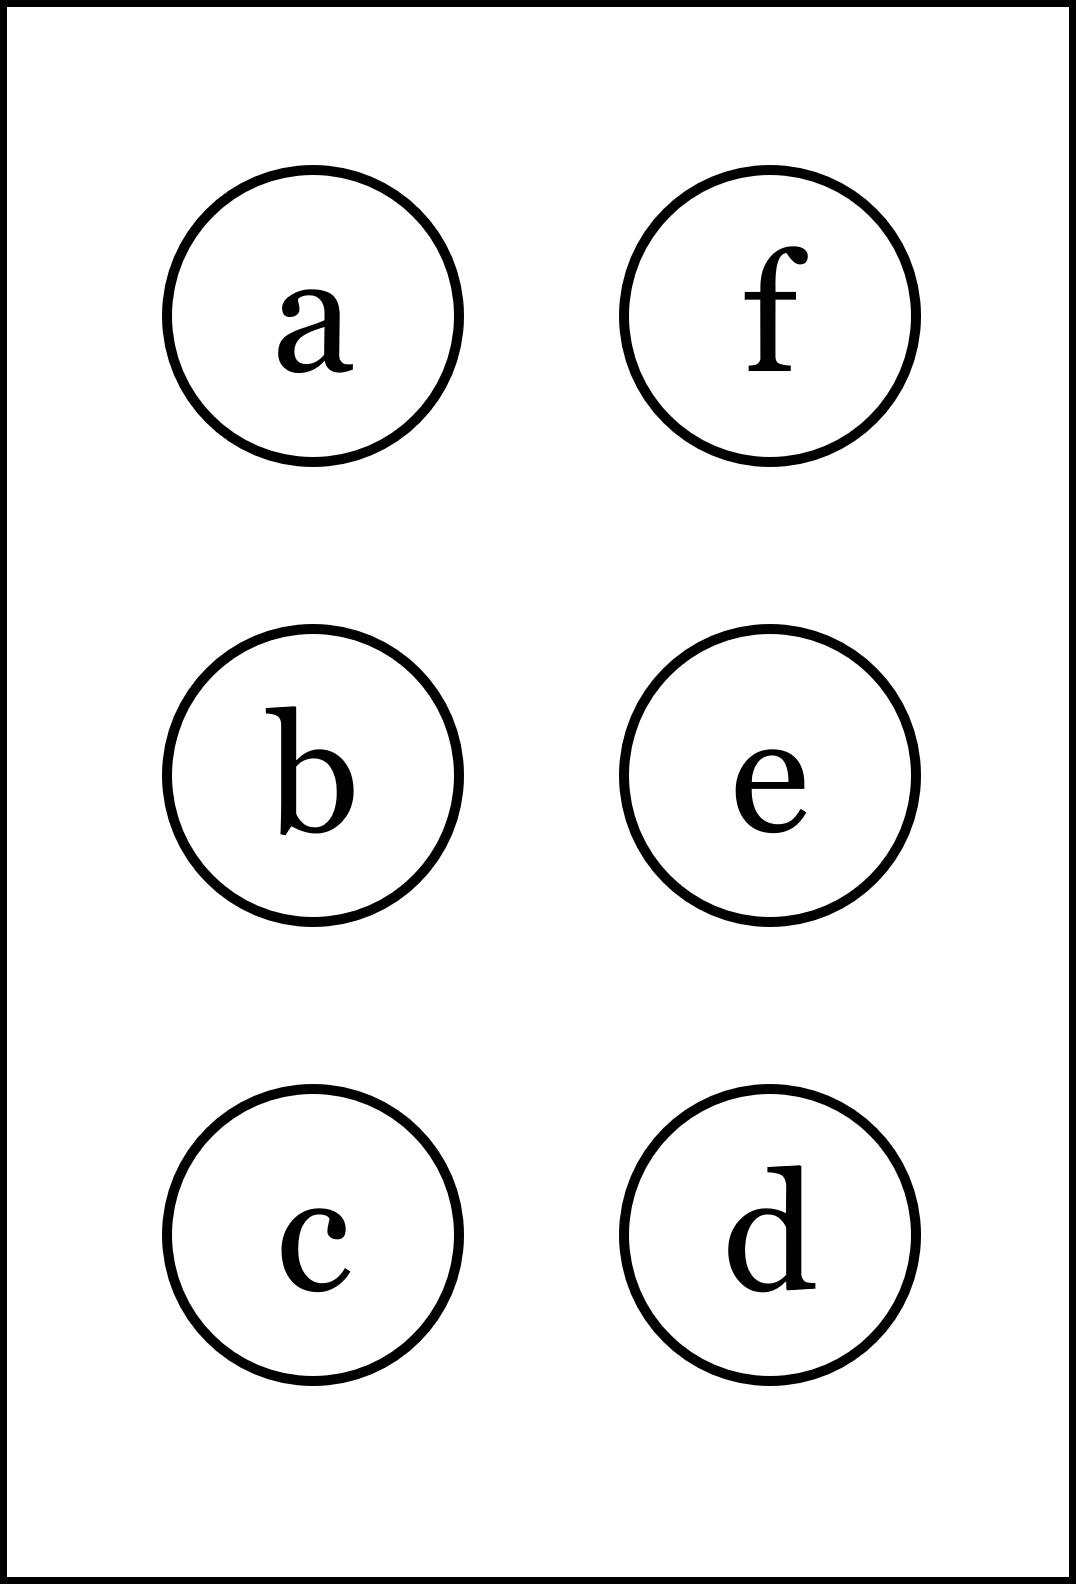
\includegraphics[height=40mm]{../images/braille.png}
{\small Písmeno Braillovej abecedy}
\end{center}
\end{minipage}
\end{center}
\end{minipage}
&
\begin{minipage}[c][99mm][t]{0.49\linewidth}
\begin{center}
\vspace{7mm}
{\huge Definiční obor, skupina \textit{Alpha $\alpha$} -\romannumeral2}\\[4.5mm]
\textit{Meno:}\phantom{xxxxxxxxxxxxxxxxxxxxxxxxxxxxxxxxxxxxxxxxxxxxxxxxxxxxxxxxxxxxxxxxx}\\[3.5mm]
\textbf{Zjisti definiční obor} zadaných funkcí. Pokud se shoduje s tím za otazníky,\\tak napravo obarvi příslušející kroužek načerno. \textbf{Spolu odevzdejte výsledné slovo}.\\[3mm]
\begin{minipage}{0.77\linewidth}
\begin{center}
\begin{varwidth}{\textwidth}
\begin{enumerate}
\normalsize
\item $f(x)=\cfrac{-2x+3}{2x-4}$\quad \dotfill\; ???\;\dotfill \quad $\mathbb{R}\smallsetminus\{2\}$
\item $f(x)=\cfrac{1}{-x^3-x^2+25x+25}$\quad \dotfill\; ???\;\dotfill \quad $\mathbb{R}\smallsetminus\{1,-5,7\}$
\item $f(x)=-3\sqrt{7x-6}$\quad \dotfill\; ???\;\dotfill \quad $x\leq\nicefrac{6}{7}$
\item $f(x)=\sqrt{-x^2-4x}$\quad \dotfill\; ???\;\dotfill \quad $x\in\langle0 , 4\rangle$
\item $f(x)=2\ln{(-8x+4)}$\quad \dotfill\; ???\;\dotfill \quad $x<\nicefrac{1}{2}$
\item $f(x)=\ln{(x^2+4x+3)}$\quad \dotfill\; ???\;\dotfill \quad $x\in(-3 , -1)$
\end{enumerate}
\end{varwidth}
\end{center}
\end{minipage}
\begin{minipage}{0.20\linewidth}
\begin{center}
{\Huge\bfseries 2.} \\[2mm]
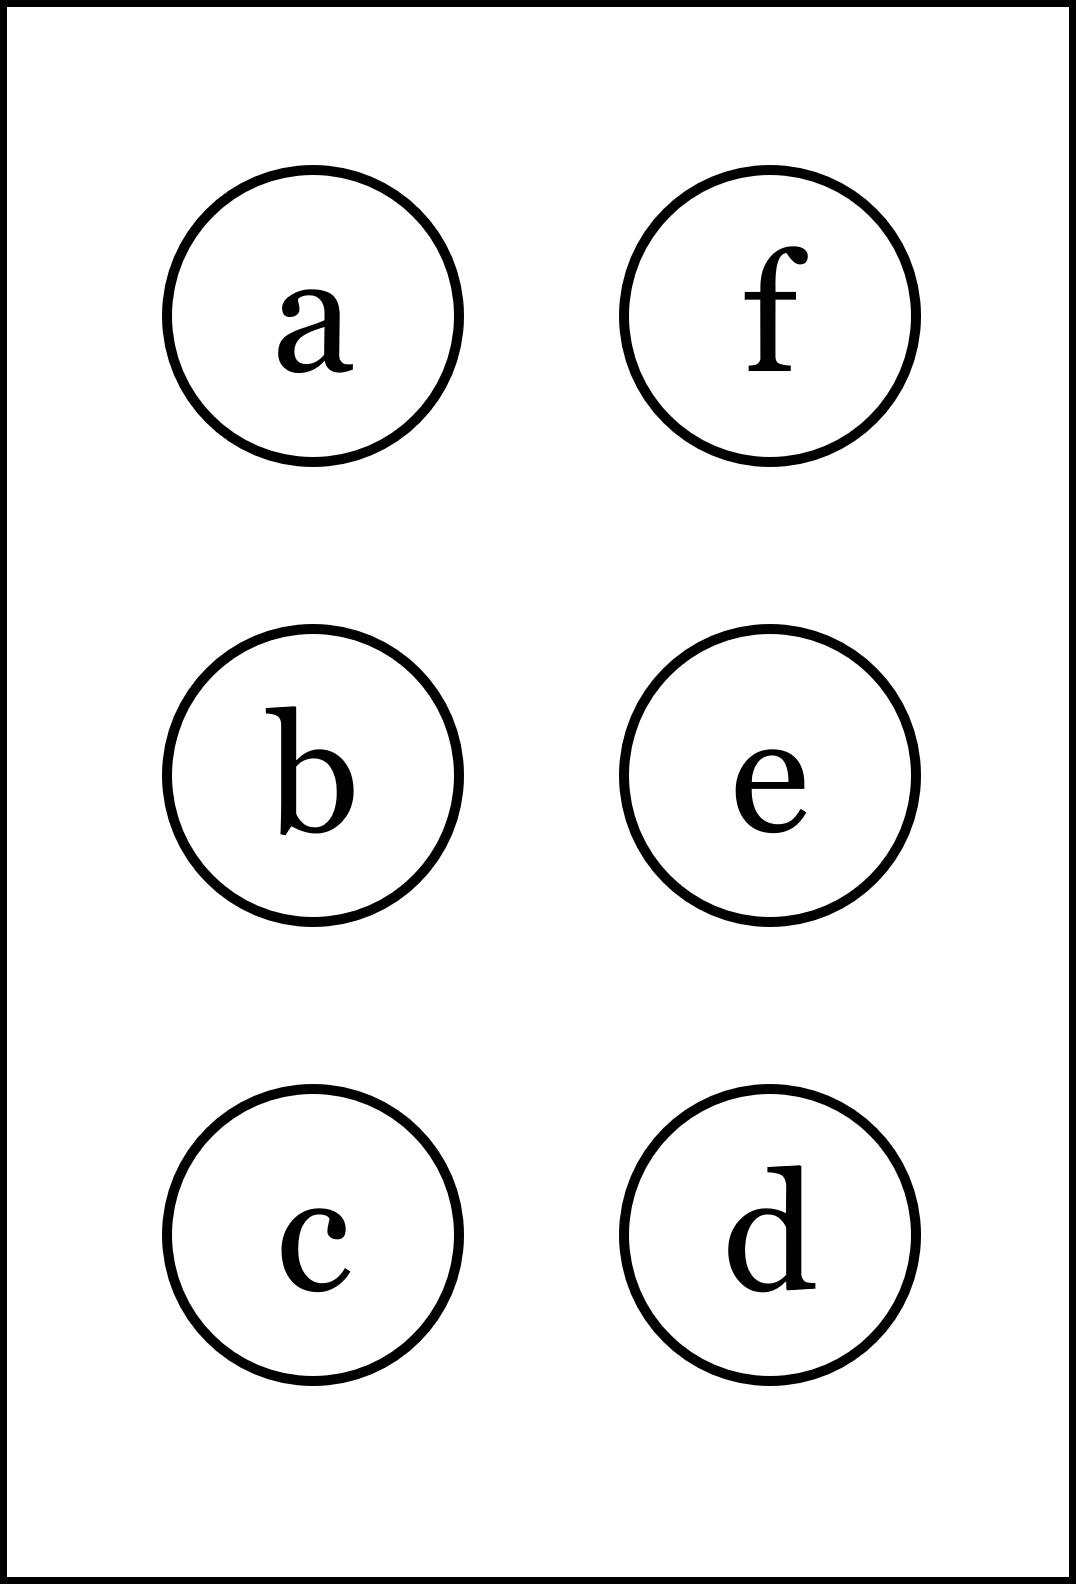
\includegraphics[height=40mm]{../images/braille.png}
{\small Písmeno Braillovej abecedy}
\end{center}
\end{minipage}
\end{center}
\end{minipage}
\\ \hdashline
\begin{minipage}[c][99mm][t]{0.49\linewidth}
\begin{center}
\vspace{7mm}
{\huge Definiční obor, skupina \textit{Alpha $\alpha$} -\romannumeral3}\\[4.5mm]
\textit{Meno:}\phantom{xxxxxxxxxxxxxxxxxxxxxxxxxxxxxxxxxxxxxxxxxxxxxxxxxxxxxxxxxxxxxxxxx}\\[3.5mm]
\textbf{Zjisti definiční obor} zadaných funkcí. Pokud se shoduje s tím za otazníky,\\tak napravo obarvi příslušející kroužek načerno. \textbf{Spolu odevzdejte výsledné slovo}.\\[3mm]
\begin{minipage}{0.77\linewidth}
\begin{center}
\begin{varwidth}{\textwidth}
\begin{enumerate}
\normalsize
\item $f(x)=\cfrac{2x-3}{6x+6}$\quad \dotfill\; ???\;\dotfill \quad $\mathbb{R}\smallsetminus\{-1\}$
\item $f(x)=\cfrac{1}{x^3-5x^2+7x-3}$\quad \dotfill\; ???\;\dotfill \quad $\mathbb{R}\smallsetminus\{1,3\}$
\item $f(x)=4\sqrt{-3x+5}$\quad \dotfill\; ???\;\dotfill \quad $x\leq\nicefrac{5}{3}$
\item $f(x)=\sqrt{-x^2-3x}$\quad \dotfill\; ???\;\dotfill \quad $x\in(-3 , 0)$
\item $f(x)=-1\ln{(-3x+8)}$\quad \dotfill\; ???\;\dotfill \quad $x>\nicefrac{8}{3}$
\item $f(x)=\ln{(x^2-4x+3)}$\quad \dotfill\; ???\;\dotfill \quad $x\in(1 , 3)$
\end{enumerate}
\end{varwidth}
\end{center}
\end{minipage}
\begin{minipage}{0.20\linewidth}
\begin{center}
{\Huge\bfseries 3.} \\[2mm]
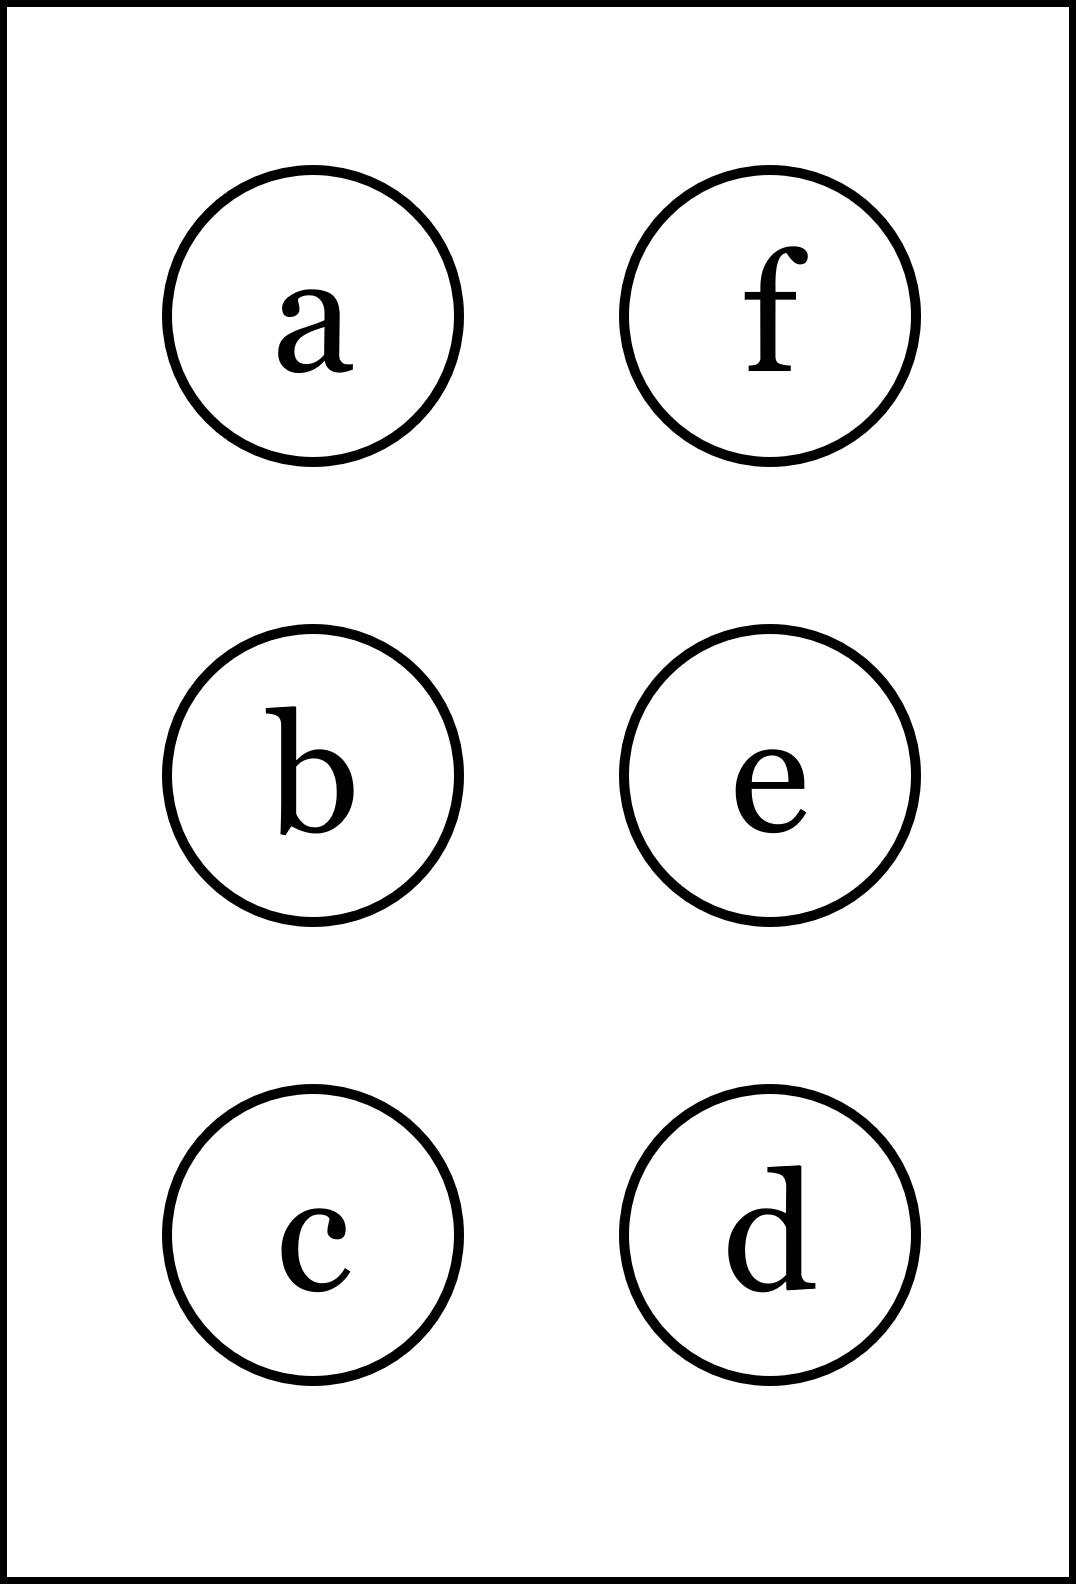
\includegraphics[height=40mm]{../images/braille.png}
{\small Písmeno Braillovej abecedy}
\end{center}
\end{minipage}
\end{center}
\end{minipage}
&
\begin{minipage}[c][99mm][t]{0.49\linewidth}
\begin{center}
\vspace{7mm}
{\huge Definiční obor, skupina \textit{Alpha $\alpha$} -\romannumeral4}\\[4.5mm]
\textit{Meno:}\phantom{xxxxxxxxxxxxxxxxxxxxxxxxxxxxxxxxxxxxxxxxxxxxxxxxxxxxxxxxxxxxxxxxx}\\[3.5mm]
\textbf{Zjisti definiční obor} zadaných funkcí. Pokud se shoduje s tím za otazníky,\\tak napravo obarvi příslušející kroužek načerno. \textbf{Spolu odevzdejte výsledné slovo}.\\[3mm]
\begin{minipage}{0.77\linewidth}
\begin{center}
\begin{varwidth}{\textwidth}
\begin{enumerate}
\normalsize
\item $f(x)=\cfrac{2x-2}{-6x+3}$\quad \dotfill\; ???\;\dotfill \quad $\mathbb{R}\smallsetminus\{\nicefrac{-1}{2}\}$
\item $f(x)=\cfrac{1}{-x^3-9x^2-14x+24}$\quad \dotfill\; ???\;\dotfill \quad $\mathbb{R}\smallsetminus\{0,-4,6\}$
\item $f(x)=-5\sqrt{5x-8}$\quad \dotfill\; ???\;\dotfill \quad $x\geq\nicefrac{8}{5}$
\item $f(x)=\sqrt{-x^2-3x}$\quad \dotfill\; ???\;\dotfill \quad $x\in(-3 , 0)$
\item $f(x)=4\ln{(9x-1)}$\quad \dotfill\; ???\;\dotfill \quad $x<\nicefrac{1}{9}$
\item $f(x)=\ln{(x^2-16)}$\quad \dotfill\; ???\;\dotfill \quad $x\in(-\infty , -4)\cup(4 , \infty)$
\end{enumerate}
\end{varwidth}
\end{center}
\end{minipage}
\begin{minipage}{0.20\linewidth}
\begin{center}
{\Huge\bfseries 4.} \\[2mm]
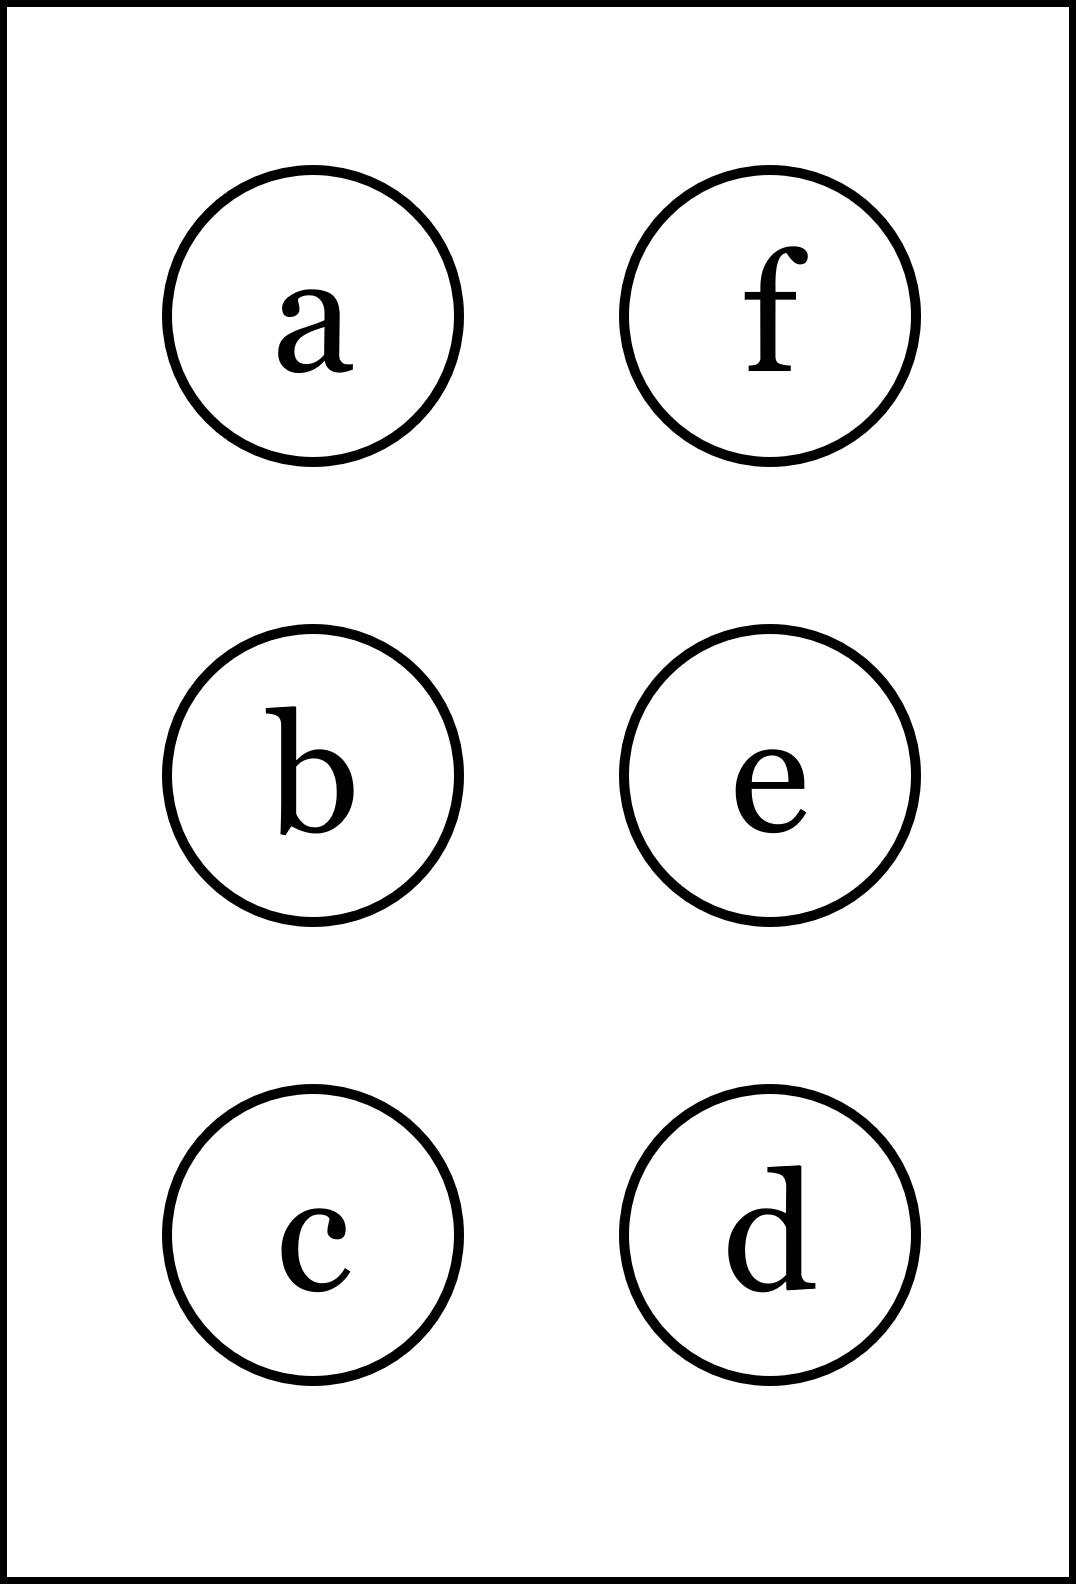
\includegraphics[height=40mm]{../images/braille.png}
{\small Písmeno Braillovej abecedy}
\end{center}
\end{minipage}
\end{center}
\end{minipage}
%
\end{tabular}
\begin{tikzpicture}[remember picture,overlay]\node[xshift=7mm,yshift=-100.6mm,anchor=north west] at (current page.north west){\ding{33}};\end{tikzpicture}
\begin{tikzpicture}[remember picture,overlay]\node[xshift=151.2mm,yshift=-7mm,anchor=north west,rotate=270] at (current page.north west){\ding{33}};\end{tikzpicture}
\newpage
\thispagestyle{empty}
\begin{tabular}{c:c}
\begin{minipage}[c][99mm][t]{0.49\linewidth}
\begin{center}
\vspace{7mm}
{\huge Definiční obor, skupina \textit{Beta $\beta$} -\romannumeral1}\\[4.5mm]
\textit{Meno:}\phantom{xxxxxxxxxxxxxxxxxxxxxxxxxxxxxxxxxxxxxxxxxxxxxxxxxxxxxxxxxxxxxxxxx}\\[3.5mm]
\textbf{Zjisti definiční obor} zadaných funkcí. Pokud se shoduje s tím za otazníky,\\tak napravo obarvi příslušející kroužek načerno. \textbf{Spolu odevzdejte výsledné slovo}.\\[3mm]
\begin{minipage}{0.77\linewidth}
\begin{center}
\begin{varwidth}{\textwidth}
\begin{enumerate}
\normalsize
\item $f(x)=\cfrac{5x+2}{2x-5}$\quad \dotfill\; ???\;\dotfill \quad $\mathbb{R}\smallsetminus\{\nicefrac{5}{2}\}$
\item $f(x)=\cfrac{1}{-x^3+4x^2+9x-36}$\quad \dotfill\; ???\;\dotfill \quad $\mathbb{R}\smallsetminus\{3,4,-3\}$
\item $f(x)=4\sqrt{x-4}$\quad \dotfill\; ???\;\dotfill \quad $x\geq4$
\item $f(x)=\sqrt{-x^2+3x}$\quad \dotfill\; ???\;\dotfill \quad $x\in\langle-3 , 0\rangle$
\item $f(x)=-4\ln{(5x-5)}$\quad \dotfill\; ???\;\dotfill \quad $x>1$
\item $f(x)=\ln{(x^2+x-42)}$\quad \dotfill\; ???\;\dotfill \quad $x\in(-7 , 6)$
\end{enumerate}
\end{varwidth}
\end{center}
\end{minipage}
\begin{minipage}{0.20\linewidth}
\begin{center}
{\Huge\bfseries 1.} \\[2mm]
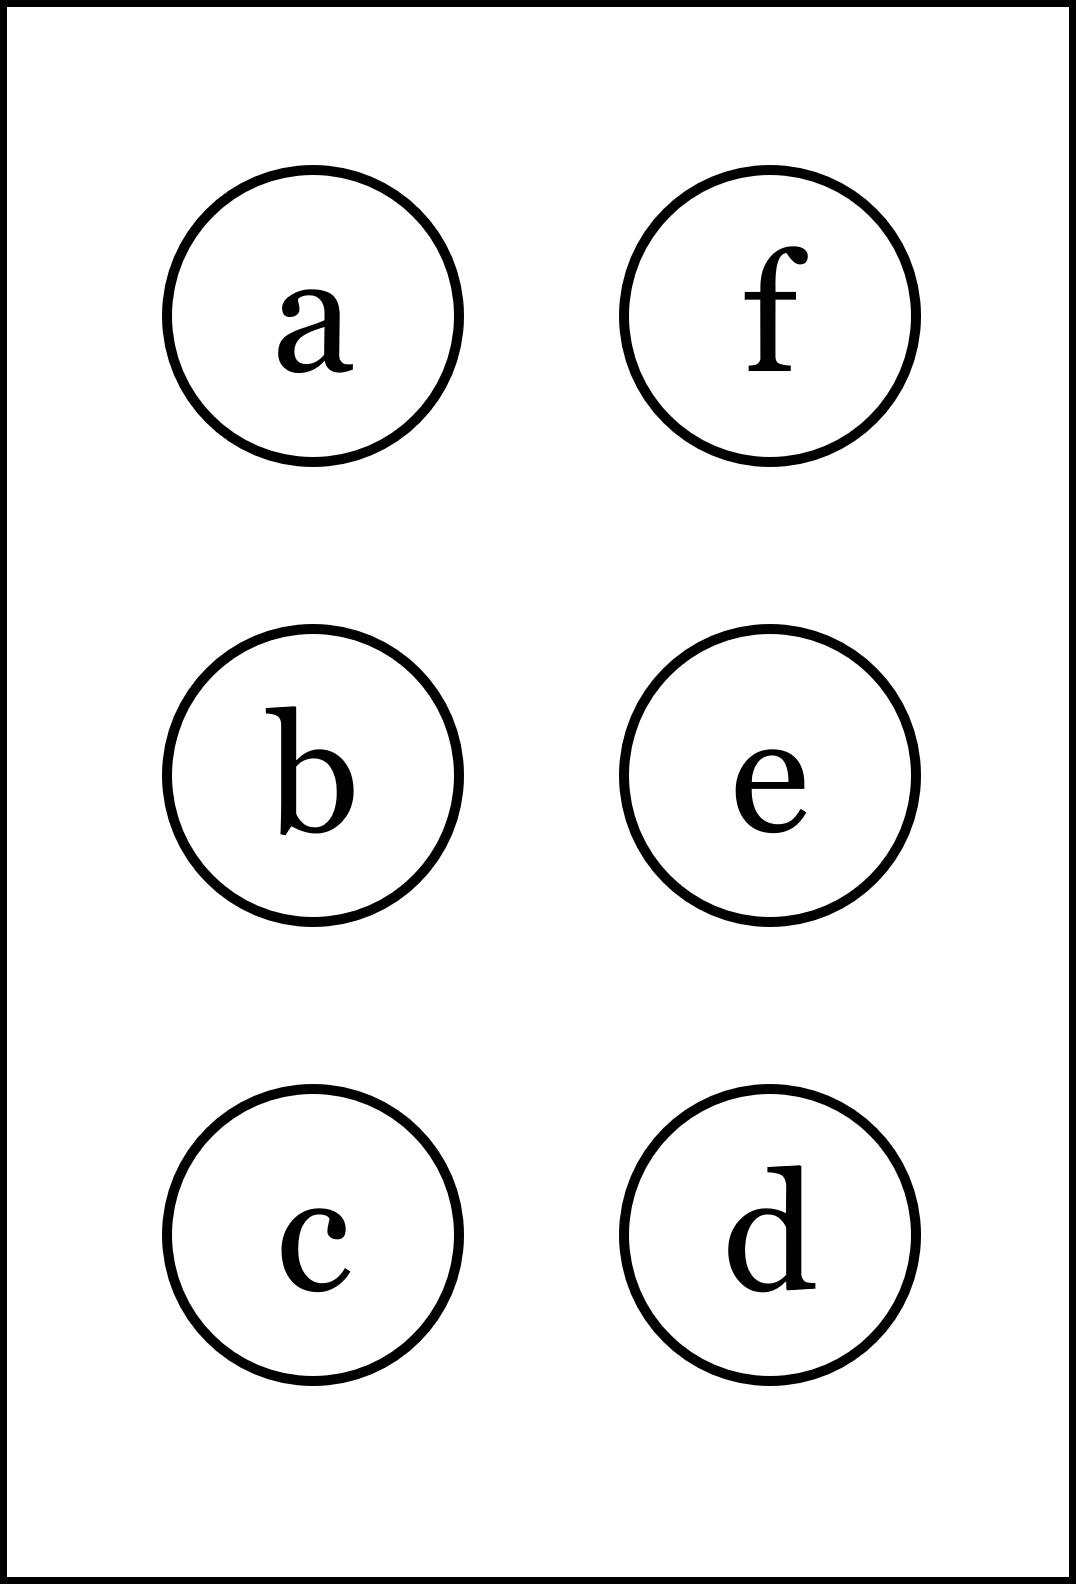
\includegraphics[height=40mm]{../images/braille.png}
{\small Písmeno Braillovej abecedy}
\end{center}
\end{minipage}
\end{center}
\end{minipage}
&
\begin{minipage}[c][99mm][t]{0.49\linewidth}
\begin{center}
\vspace{7mm}
{\huge Definiční obor, skupina \textit{Beta $\beta$} -\romannumeral2}\\[4.5mm]
\textit{Meno:}\phantom{xxxxxxxxxxxxxxxxxxxxxxxxxxxxxxxxxxxxxxxxxxxxxxxxxxxxxxxxxxxxxxxxx}\\[3.5mm]
\textbf{Zjisti definiční obor} zadaných funkcí. Pokud se shoduje s tím za otazníky,\\tak napravo obarvi příslušející kroužek načerno. \textbf{Spolu odevzdejte výsledné slovo}.\\[3mm]
\begin{minipage}{0.77\linewidth}
\begin{center}
\begin{varwidth}{\textwidth}
\begin{enumerate}
\normalsize
\item $f(x)=\cfrac{-7x+1}{5x-3}$\quad \dotfill\; ???\;\dotfill \quad $\mathbb{R}\smallsetminus\{\nicefrac{3}{5}\}$
\item $f(x)=\cfrac{1}{-x^3+5x^2+2x-24}$\quad \dotfill\; ???\;\dotfill \quad $\mathbb{R}\smallsetminus\{1,2,4\}$
\item $f(x)=-9\sqrt{-6x-6}$\quad \dotfill\; ???\;\dotfill \quad $x\leq-1$
\item $f(x)=\sqrt{-x^2+2x}$\quad \dotfill\; ???\;\dotfill \quad $x\in\langle0 , 2\rangle$
\item $f(x)=8\ln{(-2x+2)}$\quad \dotfill\; ???\;\dotfill \quad $x<1$
\item $f(x)=\ln{(x^2-6x+5)}$\quad \dotfill\; ???\;\dotfill \quad $x\in(-\infty , 1)\cup(5 , \infty)$
\end{enumerate}
\end{varwidth}
\end{center}
\end{minipage}
\begin{minipage}{0.20\linewidth}
\begin{center}
{\Huge\bfseries 2.} \\[2mm]
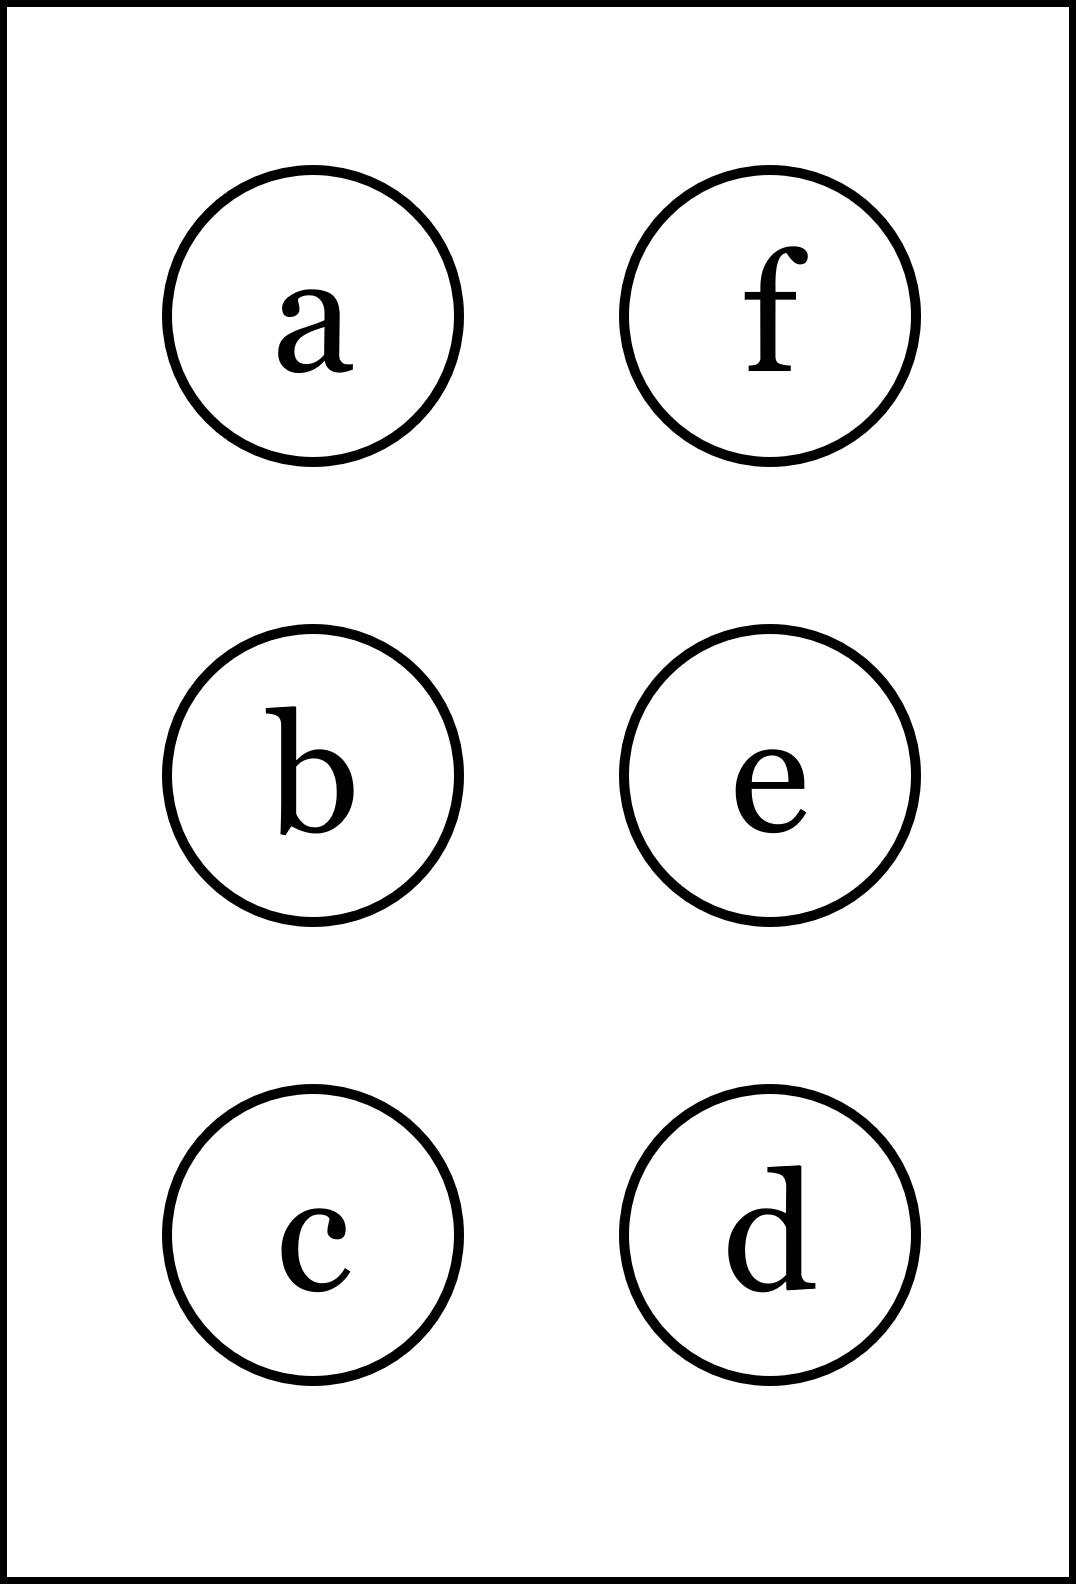
\includegraphics[height=40mm]{../images/braille.png}
{\small Písmeno Braillovej abecedy}
\end{center}
\end{minipage}
\end{center}
\end{minipage}
\\ \hdashline
\begin{minipage}[c][99mm][t]{0.49\linewidth}
\begin{center}
\vspace{7mm}
{\huge Definiční obor, skupina \textit{Beta $\beta$} -\romannumeral3}\\[4.5mm]
\textit{Meno:}\phantom{xxxxxxxxxxxxxxxxxxxxxxxxxxxxxxxxxxxxxxxxxxxxxxxxxxxxxxxxxxxxxxxxx}\\[3.5mm]
\textbf{Zjisti definiční obor} zadaných funkcí. Pokud se shoduje s tím za otazníky,\\tak napravo obarvi příslušející kroužek načerno. \textbf{Spolu odevzdejte výsledné slovo}.\\[3mm]
\begin{minipage}{0.77\linewidth}
\begin{center}
\begin{varwidth}{\textwidth}
\begin{enumerate}
\normalsize
\item $f(x)=\cfrac{6x-4}{-x+4}$\quad \dotfill\; ???\;\dotfill \quad $\mathbb{R}\smallsetminus\{4\}$
\item $f(x)=\cfrac{1}{x^3-7x^2+4x+12}$\quad \dotfill\; ???\;\dotfill \quad $\mathbb{R}\smallsetminus\{2,6,-1\}$
\item $f(x)=3\sqrt{2x+4}$\quad \dotfill\; ???\;\dotfill \quad $x\leq-2$
\item $f(x)=\sqrt{-x^2-5x}$\quad \dotfill\; ???\;\dotfill \quad $x\in(-5 , 0)$
\item $f(x)=1\ln{(-2x-3)}$\quad \dotfill\; ???\;\dotfill \quad $x<\nicefrac{3}{2}$
\item $f(x)=\ln{(x^2+2x-3)}$\quad \dotfill\; ???\;\dotfill \quad $x\in(-3 , 1)$
\end{enumerate}
\end{varwidth}
\end{center}
\end{minipage}
\begin{minipage}{0.20\linewidth}
\begin{center}
{\Huge\bfseries 3.} \\[2mm]
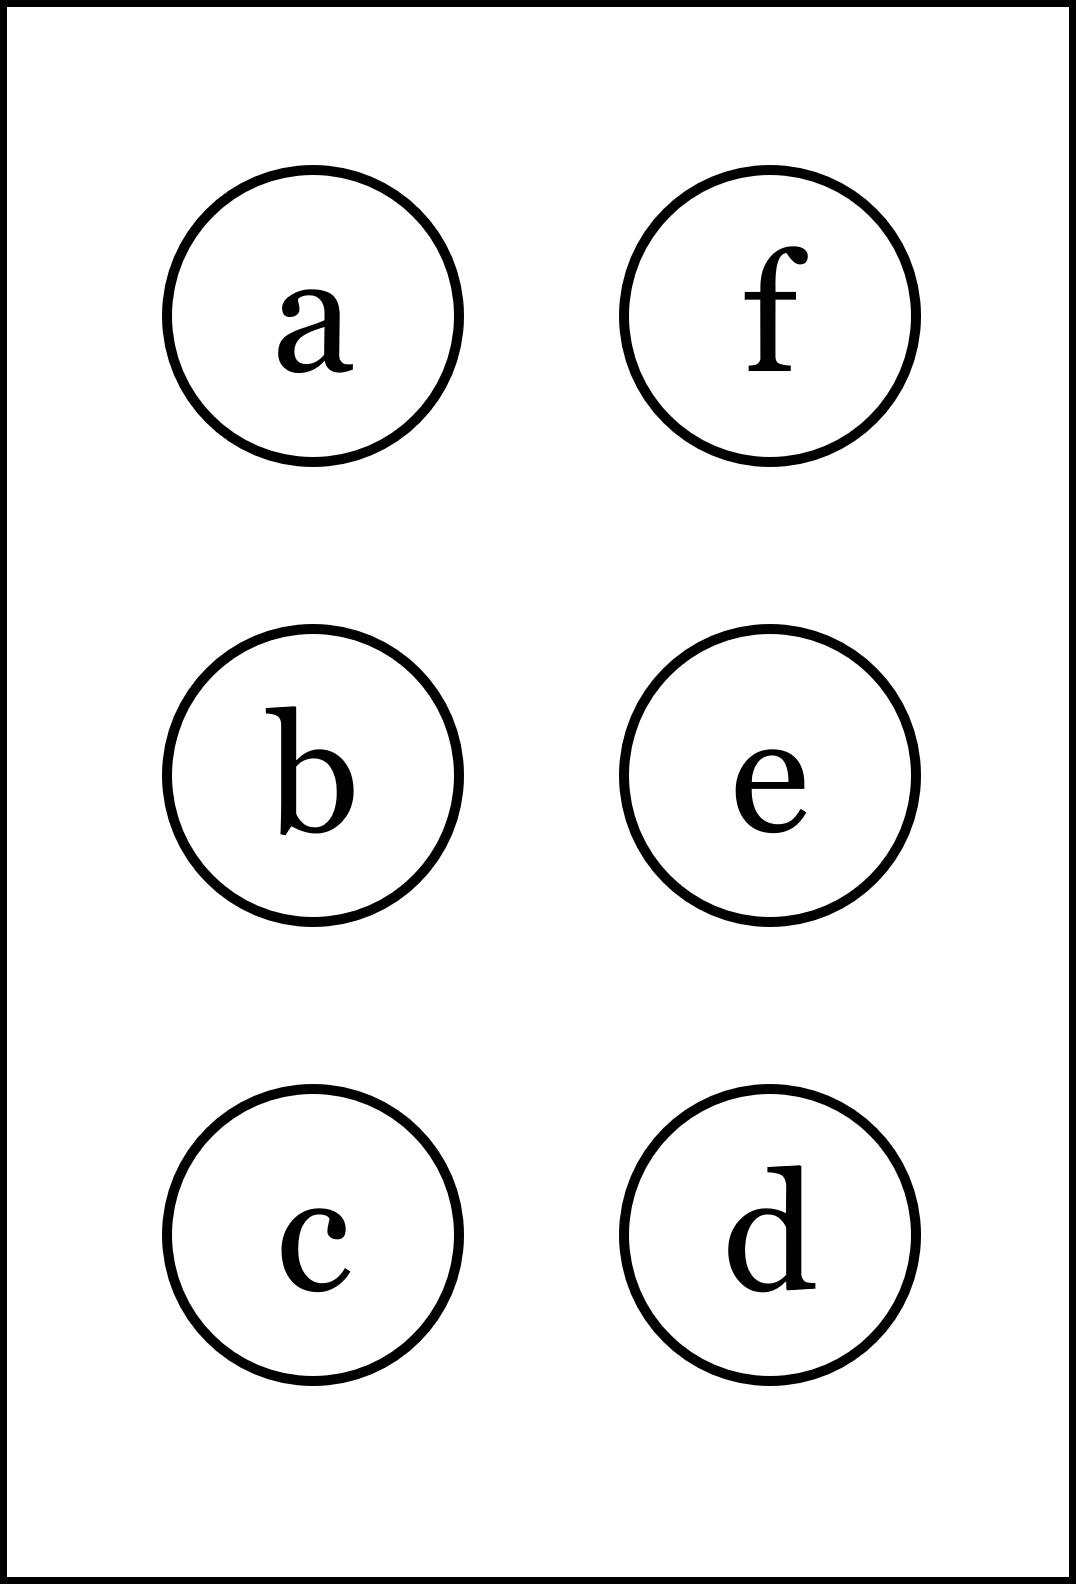
\includegraphics[height=40mm]{../images/braille.png}
{\small Písmeno Braillovej abecedy}
\end{center}
\end{minipage}
\end{center}
\end{minipage}
&
\begin{minipage}[c][99mm][t]{0.49\linewidth}
\begin{center}
\vspace{7mm}
{\huge Definiční obor, skupina \textit{Beta $\beta$} -\romannumeral4}\\[4.5mm]
\textit{Meno:}\phantom{xxxxxxxxxxxxxxxxxxxxxxxxxxxxxxxxxxxxxxxxxxxxxxxxxxxxxxxxxxxxxxxxx}\\[3.5mm]
\textbf{Zjisti definiční obor} zadaných funkcí. Pokud se shoduje s tím za otazníky,\\tak napravo obarvi příslušející kroužek načerno. \textbf{Spolu odevzdejte výsledné slovo}.\\[3mm]
\begin{minipage}{0.77\linewidth}
\begin{center}
\begin{varwidth}{\textwidth}
\begin{enumerate}
\normalsize
\item $f(x)=\cfrac{-7x+5}{-x-1}$\quad \dotfill\; ???\;\dotfill \quad $\mathbb{R}\smallsetminus\{-1\}$
\item $f(x)=\cfrac{1}{x^3-5x^2+2x+8}$\quad \dotfill\; ???\;\dotfill \quad $\mathbb{R}\smallsetminus\{0,-4,-1\}$
\item $f(x)=-1\sqrt{8x-1}$\quad \dotfill\; ???\;\dotfill \quad $x\leq\nicefrac{1}{8}$
\item $f(x)=\sqrt{-x^2+x}$\quad \dotfill\; ???\;\dotfill \quad $x\in\langle-1 , 0\rangle$
\item $f(x)=-9\ln{(-5x-3)}$\quad \dotfill\; ???\;\dotfill \quad $x>\nicefrac{-3}{5}$
\item $f(x)=\ln{(x^2+2x-8)}$\quad \dotfill\; ???\;\dotfill \quad $x\in(-4 , 2)$
\end{enumerate}
\end{varwidth}
\end{center}
\end{minipage}
\begin{minipage}{0.20\linewidth}
\begin{center}
{\Huge\bfseries 4.} \\[2mm]
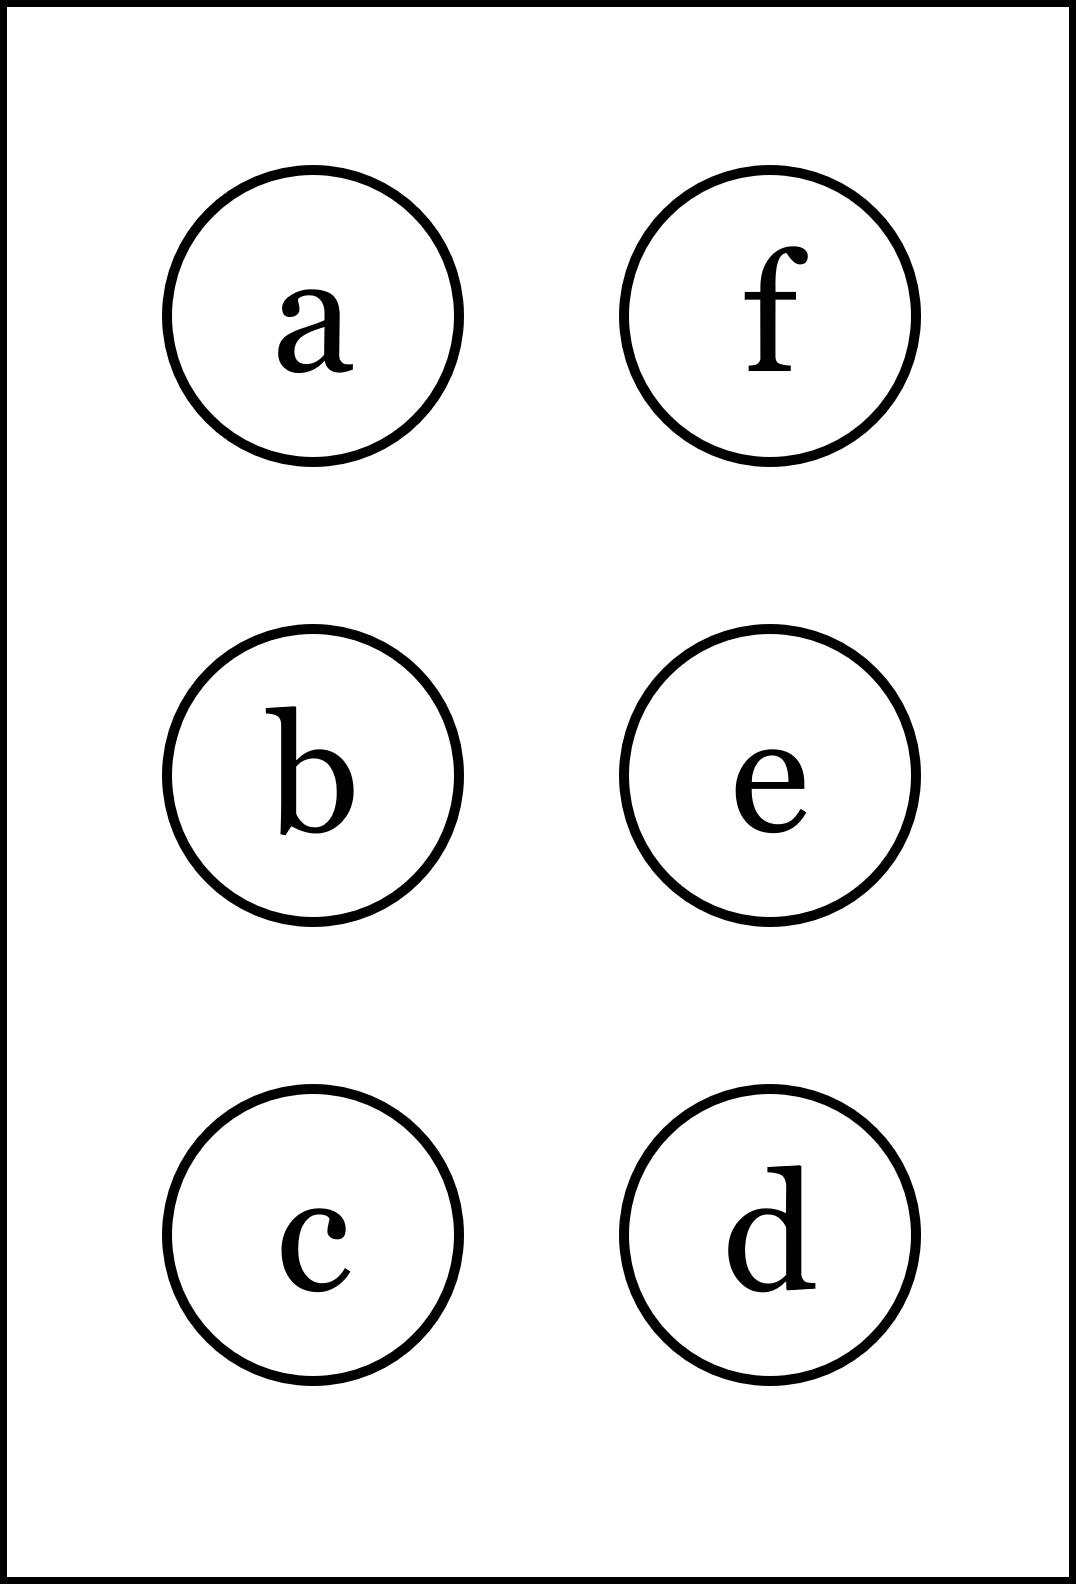
\includegraphics[height=40mm]{../images/braille.png}
{\small Písmeno Braillovej abecedy}
\end{center}
\end{minipage}
\end{center}
\end{minipage}
%
\end{tabular}
\begin{tikzpicture}[remember picture,overlay]\node[xshift=7mm,yshift=-100.6mm,anchor=north west] at (current page.north west){\ding{33}};\end{tikzpicture}
\begin{tikzpicture}[remember picture,overlay]\node[xshift=151.2mm,yshift=-7mm,anchor=north west,rotate=270] at (current page.north west){\ding{33}};\end{tikzpicture}
\newpage
\thispagestyle{empty}
\begin{tabular}{c:c}
\begin{minipage}[c][99mm][t]{0.49\linewidth}
\begin{center}
\vspace{7mm}
{\huge Definiční obor, skupina \textit{Gamma $\gamma$} -\romannumeral1}\\[4.5mm]
\textit{Meno:}\phantom{xxxxxxxxxxxxxxxxxxxxxxxxxxxxxxxxxxxxxxxxxxxxxxxxxxxxxxxxxxxxxxxxx}\\[3.5mm]
\textbf{Zjisti definiční obor} zadaných funkcí. Pokud se shoduje s tím za otazníky,\\tak napravo obarvi příslušející kroužek načerno. \textbf{Spolu odevzdejte výsledné slovo}.\\[3mm]
\begin{minipage}{0.77\linewidth}
\begin{center}
\begin{varwidth}{\textwidth}
\begin{enumerate}
\normalsize
\item $f(x)=\cfrac{7x-4}{4x-3}$\quad \dotfill\; ???\;\dotfill \quad $\mathbb{R}\smallsetminus\{\nicefrac{3}{4}\}$
\item $f(x)=\cfrac{1}{-x^3+6x^2+31x-36}$\quad \dotfill\; ???\;\dotfill \quad $\mathbb{R}\smallsetminus\{-4,-1,7\}$
\item $f(x)=2\sqrt{2x+4}$\quad \dotfill\; ???\;\dotfill \quad $x\geq2$
\item $f(x)=\sqrt{-x^2+x}$\quad \dotfill\; ???\;\dotfill \quad $x\in(0 , 1)$
\item $f(x)=-1\ln{(7x-5)}$\quad \dotfill\; ???\;\dotfill \quad $x>\nicefrac{-5}{7}$
\item $f(x)=\ln{(x^2-5x+4)}$\quad \dotfill\; ???\;\dotfill \quad $x\in(-\infty , 1)\cup(4 , \infty)$
\end{enumerate}
\end{varwidth}
\end{center}
\end{minipage}
\begin{minipage}{0.20\linewidth}
\begin{center}
{\Huge\bfseries 1.} \\[2mm]
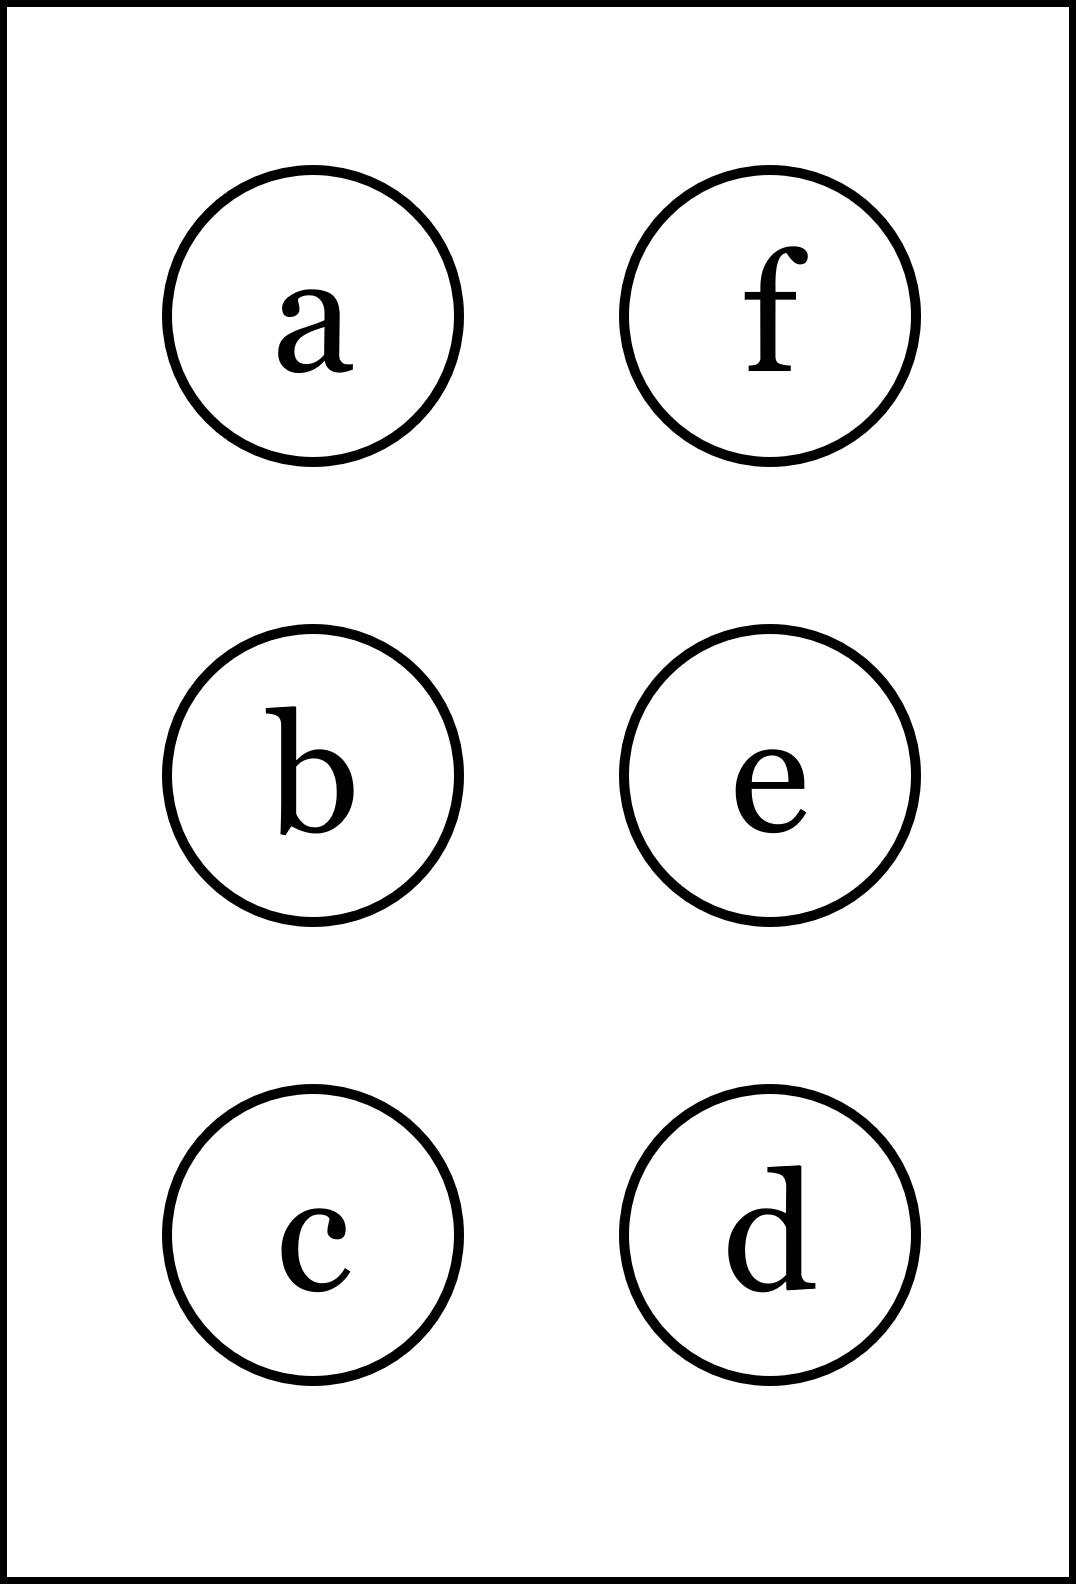
\includegraphics[height=40mm]{../images/braille.png}
{\small Písmeno Braillovej abecedy}
\end{center}
\end{minipage}
\end{center}
\end{minipage}
&
\begin{minipage}[c][99mm][t]{0.49\linewidth}
\begin{center}
\vspace{7mm}
{\huge Definiční obor, skupina \textit{Gamma $\gamma$} -\romannumeral2}\\[4.5mm]
\textit{Meno:}\phantom{xxxxxxxxxxxxxxxxxxxxxxxxxxxxxxxxxxxxxxxxxxxxxxxxxxxxxxxxxxxxxxxxx}\\[3.5mm]
\textbf{Zjisti definiční obor} zadaných funkcí. Pokud se shoduje s tím za otazníky,\\tak napravo obarvi příslušející kroužek načerno. \textbf{Spolu odevzdejte výsledné slovo}.\\[3mm]
\begin{minipage}{0.77\linewidth}
\begin{center}
\begin{varwidth}{\textwidth}
\begin{enumerate}
\normalsize
\item $f(x)=\cfrac{4x-2}{-7x+7}$\quad \dotfill\; ???\;\dotfill \quad $\mathbb{R}\smallsetminus\{1\}$
\item $f(x)=\cfrac{1}{-x^3+5x^2+17x-21}$\quad \dotfill\; ???\;\dotfill \quad $\mathbb{R}\smallsetminus\{9,-3,-1\}$
\item $f(x)=-5\sqrt{-2x+3}$\quad \dotfill\; ???\;\dotfill \quad $x\leq\nicefrac{3}{2}$
\item $f(x)=\sqrt{-x^2+4x}$\quad \dotfill\; ???\;\dotfill \quad $x\in\langle0 , 4\rangle$
\item $f(x)=1\ln{(-6x+1)}$\quad \dotfill\; ???\;\dotfill \quad $x<\nicefrac{-1}{6}$
\item $f(x)=\ln{(x^2-2x+1)}$\quad \dotfill\; ???\;\dotfill \quad $x\in(1 , 1)$
\end{enumerate}
\end{varwidth}
\end{center}
\end{minipage}
\begin{minipage}{0.20\linewidth}
\begin{center}
{\Huge\bfseries 2.} \\[2mm]
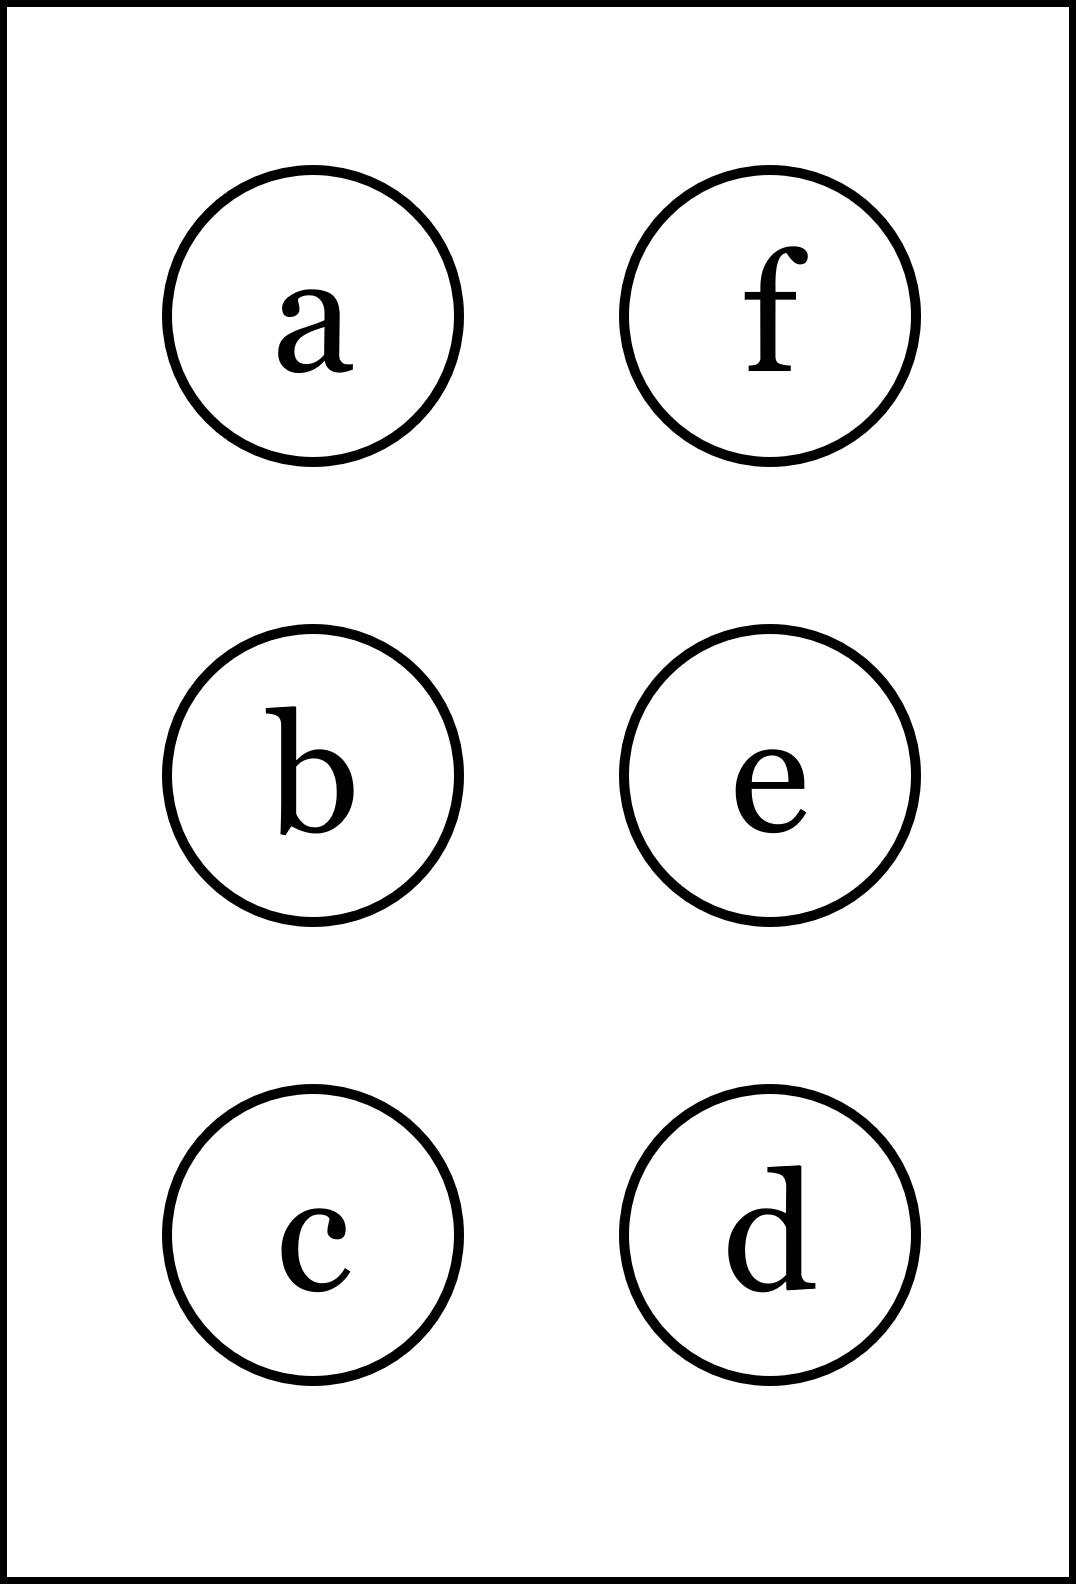
\includegraphics[height=40mm]{../images/braille.png}
{\small Písmeno Braillovej abecedy}
\end{center}
\end{minipage}
\end{center}
\end{minipage}
\\ \hdashline
\begin{minipage}[c][99mm][t]{0.49\linewidth}
\begin{center}
\vspace{7mm}
{\huge Definiční obor, skupina \textit{Gamma $\gamma$} -\romannumeral3}\\[4.5mm]
\textit{Meno:}\phantom{xxxxxxxxxxxxxxxxxxxxxxxxxxxxxxxxxxxxxxxxxxxxxxxxxxxxxxxxxxxxxxxxx}\\[3.5mm]
\textbf{Zjisti definiční obor} zadaných funkcí. Pokud se shoduje s tím za otazníky,\\tak napravo obarvi příslušející kroužek načerno. \textbf{Spolu odevzdejte výsledné slovo}.\\[3mm]
\begin{minipage}{0.77\linewidth}
\begin{center}
\begin{varwidth}{\textwidth}
\begin{enumerate}
\normalsize
\item $f(x)=\cfrac{-6x+3}{-x+1}$\quad \dotfill\; ???\;\dotfill \quad $\mathbb{R}\smallsetminus\{1\}$
\item $f(x)=\cfrac{1}{-8x^3+16x^2+8x-16}$\quad \dotfill\; ???\;\dotfill \quad $\mathbb{R}\smallsetminus\{0,2,-1\}$
\item $f(x)=5\sqrt{3x-2}$\quad \dotfill\; ???\;\dotfill \quad $x\geq\nicefrac{2}{3}$
\item $f(x)=\sqrt{-x^2-4x}$\quad \dotfill\; ???\;\dotfill \quad $x\in\langle0 , 4\rangle$
\item $f(x)=-6\ln{(3x-1)}$\quad \dotfill\; ???\;\dotfill \quad $x>\nicefrac{-1}{3}$
\item $f(x)=\ln{(x^2-7x+6)}$\quad \dotfill\; ???\;\dotfill \quad $x\in(1 , 6)$
\end{enumerate}
\end{varwidth}
\end{center}
\end{minipage}
\begin{minipage}{0.20\linewidth}
\begin{center}
{\Huge\bfseries 3.} \\[2mm]
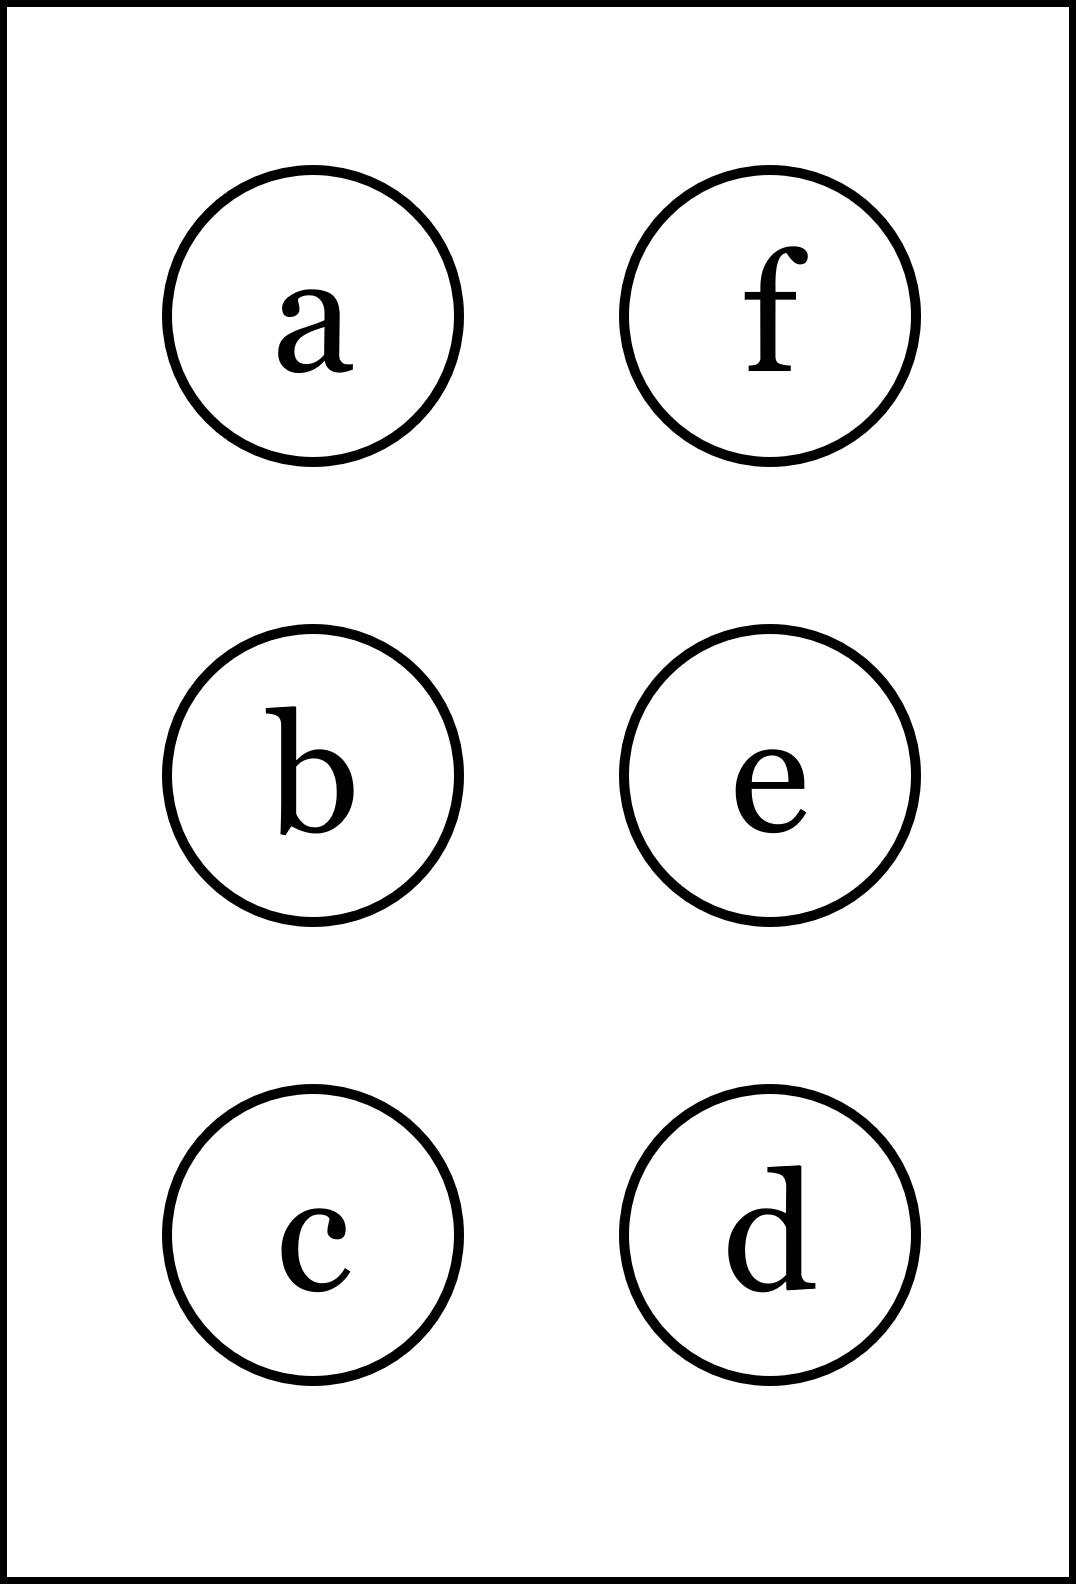
\includegraphics[height=40mm]{../images/braille.png}
{\small Písmeno Braillovej abecedy}
\end{center}
\end{minipage}
\end{center}
\end{minipage}
&
\begin{minipage}[c][99mm][t]{0.49\linewidth}
\begin{center}
\vspace{7mm}
{\huge Definiční obor, skupina \textit{Gamma $\gamma$} -\romannumeral4}\\[4.5mm]
\textit{Meno:}\phantom{xxxxxxxxxxxxxxxxxxxxxxxxxxxxxxxxxxxxxxxxxxxxxxxxxxxxxxxxxxxxxxxxx}\\[3.5mm]
\textbf{Zjisti definiční obor} zadaných funkcí. Pokud se shoduje s tím za otazníky,\\tak napravo obarvi příslušející kroužek načerno. \textbf{Spolu odevzdejte výsledné slovo}.\\[3mm]
\begin{minipage}{0.77\linewidth}
\begin{center}
\begin{varwidth}{\textwidth}
\begin{enumerate}
\normalsize
\item $f(x)=\cfrac{-2x+1}{x-5}$\quad \dotfill\; ???\;\dotfill \quad $\mathbb{R}\smallsetminus\{5\}$
\item $f(x)=\cfrac{1}{-x^3+6x^2-3x-10}$\quad \dotfill\; ???\;\dotfill \quad $\mathbb{R}\smallsetminus\{2,5,-1\}$
\item $f(x)=4\sqrt{x+4}$\quad \dotfill\; ???\;\dotfill \quad $x\geq-4$
\item $f(x)=\sqrt{-x^2+x}$\quad \dotfill\; ???\;\dotfill \quad $x\in(0 , 1)$
\item $f(x)=-1\ln{(7x-3)}$\quad \dotfill\; ???\;\dotfill \quad $x>\nicefrac{3}{7}$
\item $f(x)=\ln{(x^2+7x+12)}$\quad \dotfill\; ???\;\dotfill \quad $x\in(-4 , -3)$
\end{enumerate}
\end{varwidth}
\end{center}
\end{minipage}
\begin{minipage}{0.20\linewidth}
\begin{center}
{\Huge\bfseries 4.} \\[2mm]
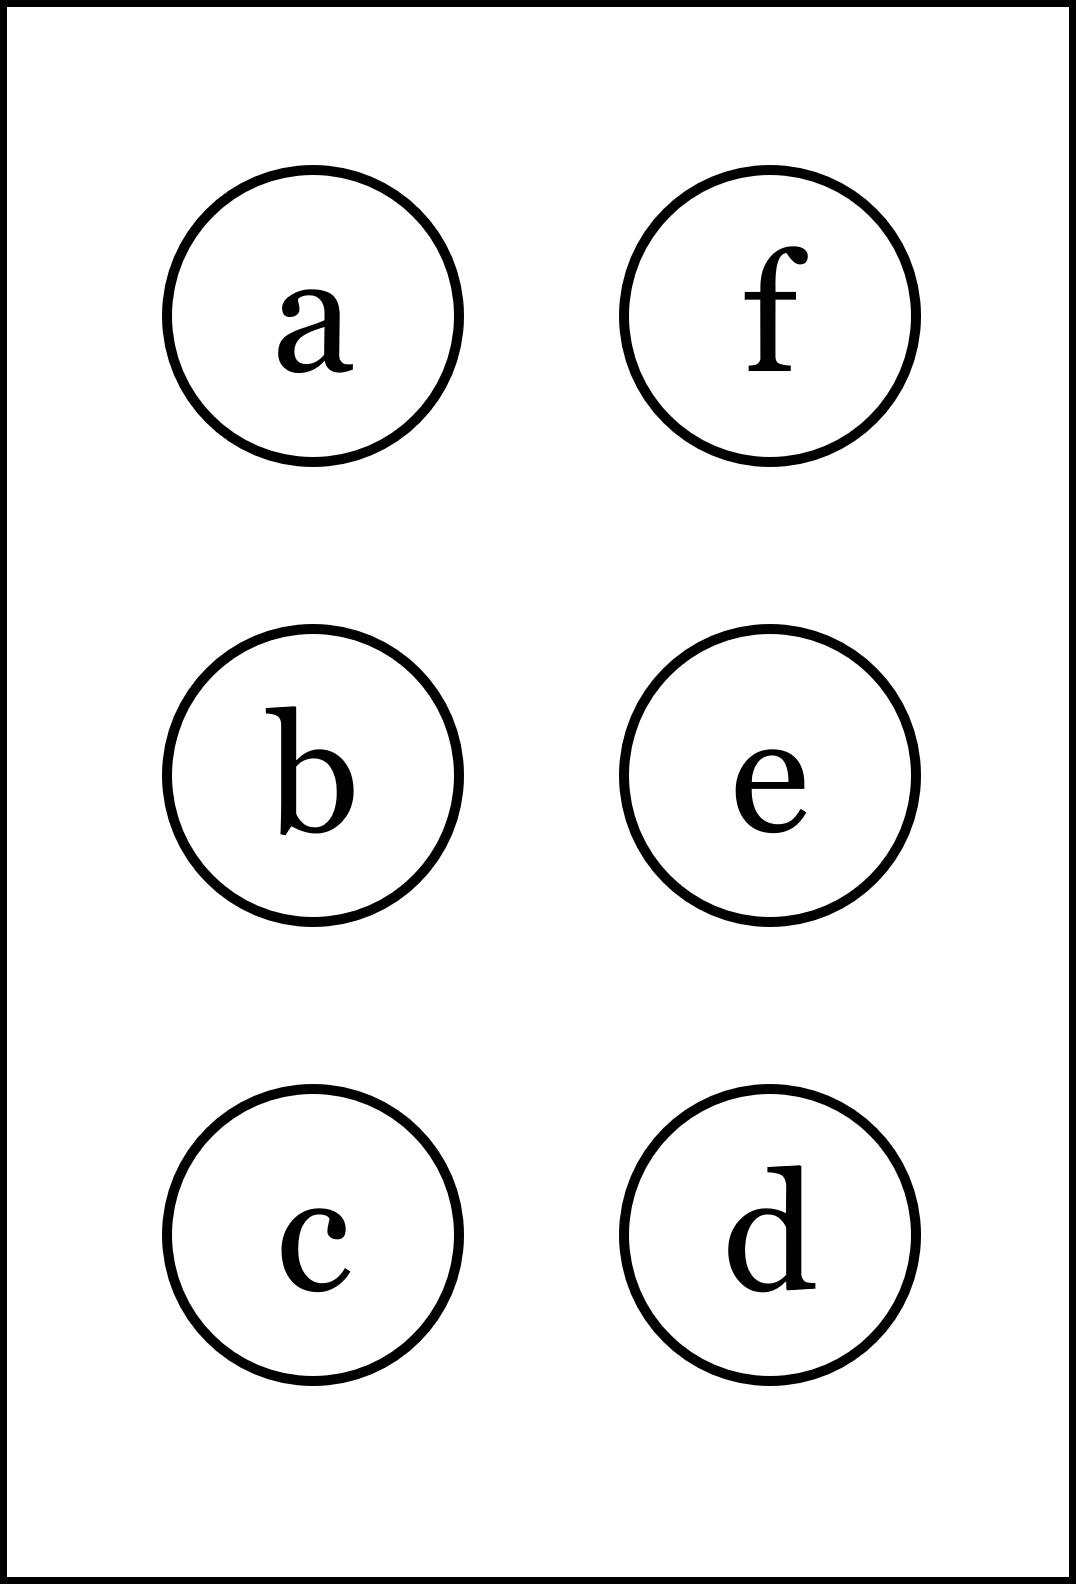
\includegraphics[height=40mm]{../images/braille.png}
{\small Písmeno Braillovej abecedy}
\end{center}
\end{minipage}
\end{center}
\end{minipage}
%
\end{tabular}
\begin{tikzpicture}[remember picture,overlay]\node[xshift=7mm,yshift=-100.6mm,anchor=north west] at (current page.north west){\ding{33}};\end{tikzpicture}
\begin{tikzpicture}[remember picture,overlay]\node[xshift=151.2mm,yshift=-7mm,anchor=north west,rotate=270] at (current page.north west){\ding{33}};\end{tikzpicture}
\newpage
\thispagestyle{empty}
\begin{tabular}{c:c}
\begin{minipage}[c][99mm][t]{0.49\linewidth}
\begin{center}
\vspace{7mm}
{\huge Definiční obor, skupina \textit{Delta $\delta$} -\romannumeral1}\\[4.5mm]
\textit{Meno:}\phantom{xxxxxxxxxxxxxxxxxxxxxxxxxxxxxxxxxxxxxxxxxxxxxxxxxxxxxxxxxxxxxxxxx}\\[3.5mm]
\textbf{Zjisti definiční obor} zadaných funkcí. Pokud se shoduje s tím za otazníky,\\tak napravo obarvi příslušející kroužek načerno. \textbf{Spolu odevzdejte výsledné slovo}.\\[3mm]
\begin{minipage}{0.77\linewidth}
\begin{center}
\begin{varwidth}{\textwidth}
\begin{enumerate}
\normalsize
\item $f(x)=\cfrac{5x-3}{4x-1}$\quad \dotfill\; ???\;\dotfill \quad $\mathbb{R}\smallsetminus\{\nicefrac{1}{4}\}$
\item $f(x)=\cfrac{1}{2x^3+10x^2+16x+8}$\quad \dotfill\; ???\;\dotfill \quad $\mathbb{R}\smallsetminus\{1,-3,-2\}$
\item $f(x)=-2\sqrt{2x-6}$\quad \dotfill\; ???\;\dotfill \quad $x\leq3$
\item $f(x)=\sqrt{-x^2+4x}$\quad \dotfill\; ???\;\dotfill \quad $x\in\langle-4 , 0\rangle$
\item $f(x)=1\ln{(-8x-1)}$\quad \dotfill\; ???\;\dotfill \quad $x<\nicefrac{1}{8}$
\item $f(x)=\ln{(x^2-4)}$\quad \dotfill\; ???\;\dotfill \quad $x\in(-\infty , -2)\cup(2 , \infty)$
\end{enumerate}
\end{varwidth}
\end{center}
\end{minipage}
\begin{minipage}{0.20\linewidth}
\begin{center}
{\Huge\bfseries 1.} \\[2mm]
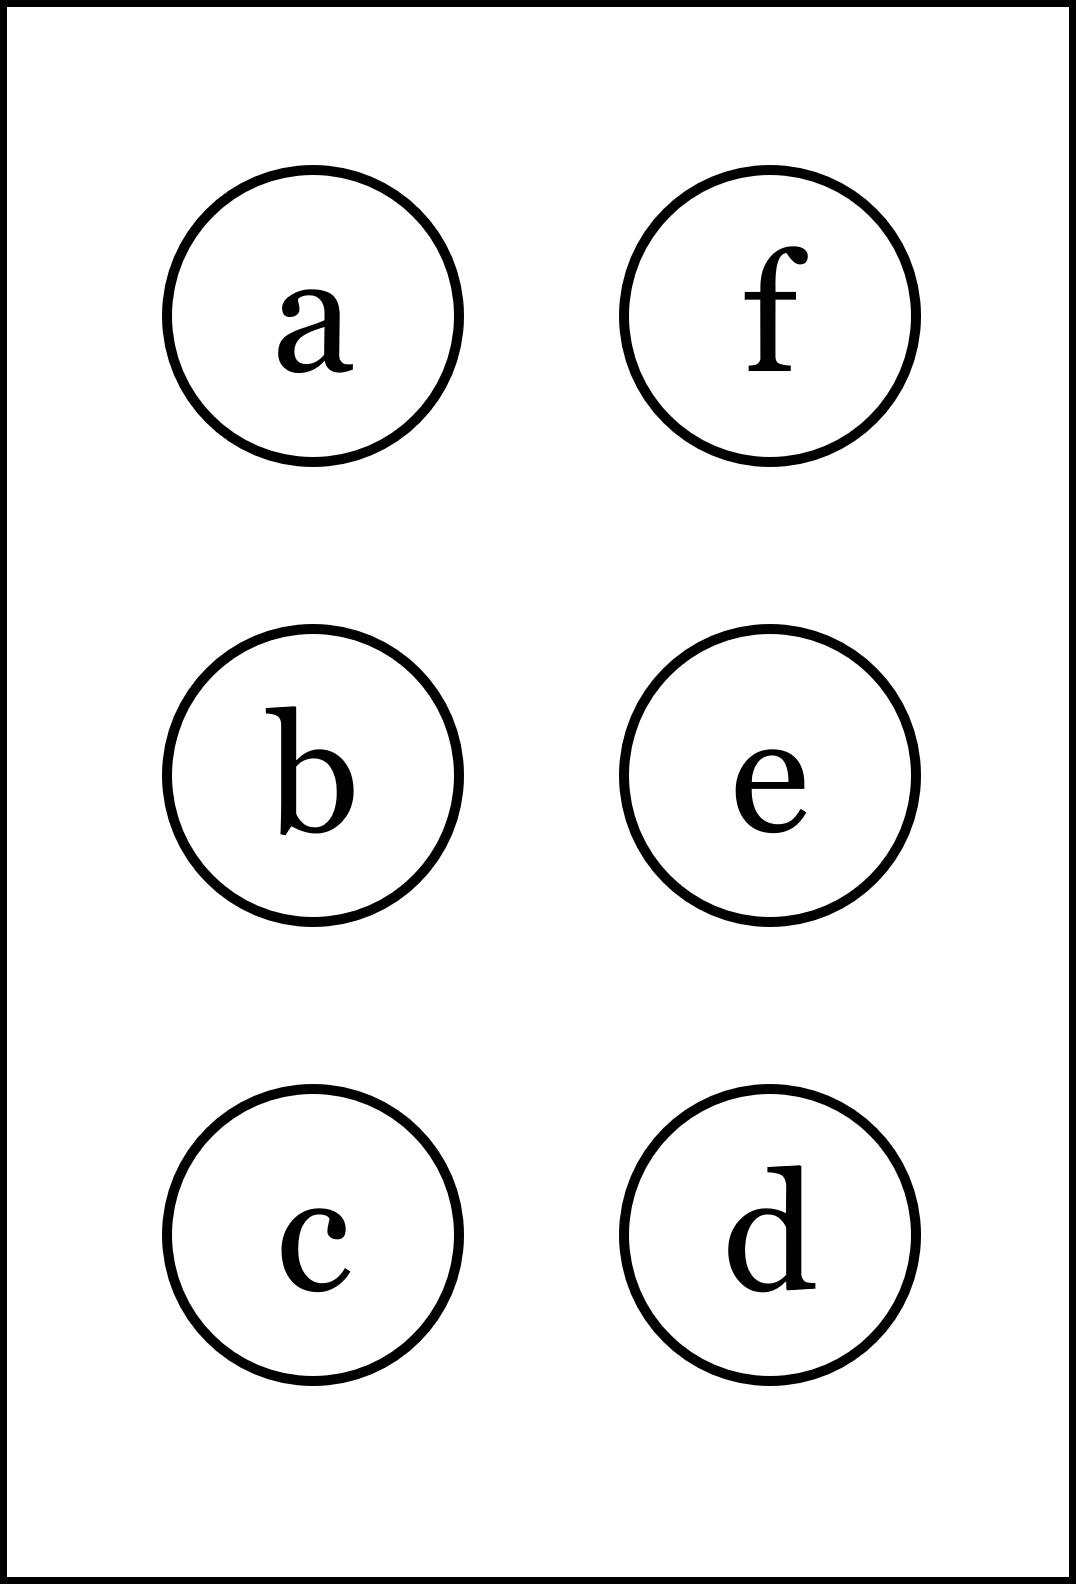
\includegraphics[height=40mm]{../images/braille.png}
{\small Písmeno Braillovej abecedy}
\end{center}
\end{minipage}
\end{center}
\end{minipage}
&
\begin{minipage}[c][99mm][t]{0.49\linewidth}
\begin{center}
\vspace{7mm}
{\huge Definiční obor, skupina \textit{Delta $\delta$} -\romannumeral2}\\[4.5mm]
\textit{Meno:}\phantom{xxxxxxxxxxxxxxxxxxxxxxxxxxxxxxxxxxxxxxxxxxxxxxxxxxxxxxxxxxxxxxxxx}\\[3.5mm]
\textbf{Zjisti definiční obor} zadaných funkcí. Pokud se shoduje s tím za otazníky,\\tak napravo obarvi příslušející kroužek načerno. \textbf{Spolu odevzdejte výsledné slovo}.\\[3mm]
\begin{minipage}{0.77\linewidth}
\begin{center}
\begin{varwidth}{\textwidth}
\begin{enumerate}
\normalsize
\item $f(x)=\cfrac{5x+2}{-x-2}$\quad \dotfill\; ???\;\dotfill \quad $\mathbb{R}\smallsetminus\{-2\}$
\item $f(x)=\cfrac{1}{-2x^3+16x^2-38x+24}$\quad \dotfill\; ???\;\dotfill \quad $\mathbb{R}\smallsetminus\{2,4,-1\}$
\item $f(x)=-3\sqrt{6x+3}$\quad \dotfill\; ???\;\dotfill \quad $x\geq\nicefrac{1}{2}$
\item $f(x)=\sqrt{-x^2+3x}$\quad \dotfill\; ???\;\dotfill \quad $x\in\langle-3 , 0\rangle$
\item $f(x)=-2\ln{(3x+4)}$\quad \dotfill\; ???\;\dotfill \quad $x>\nicefrac{-4}{3}$
\item $f(x)=\ln{(x^2-7x+6)}$\quad \dotfill\; ???\;\dotfill \quad $x\in(1 , 6)$
\end{enumerate}
\end{varwidth}
\end{center}
\end{minipage}
\begin{minipage}{0.20\linewidth}
\begin{center}
{\Huge\bfseries 2.} \\[2mm]
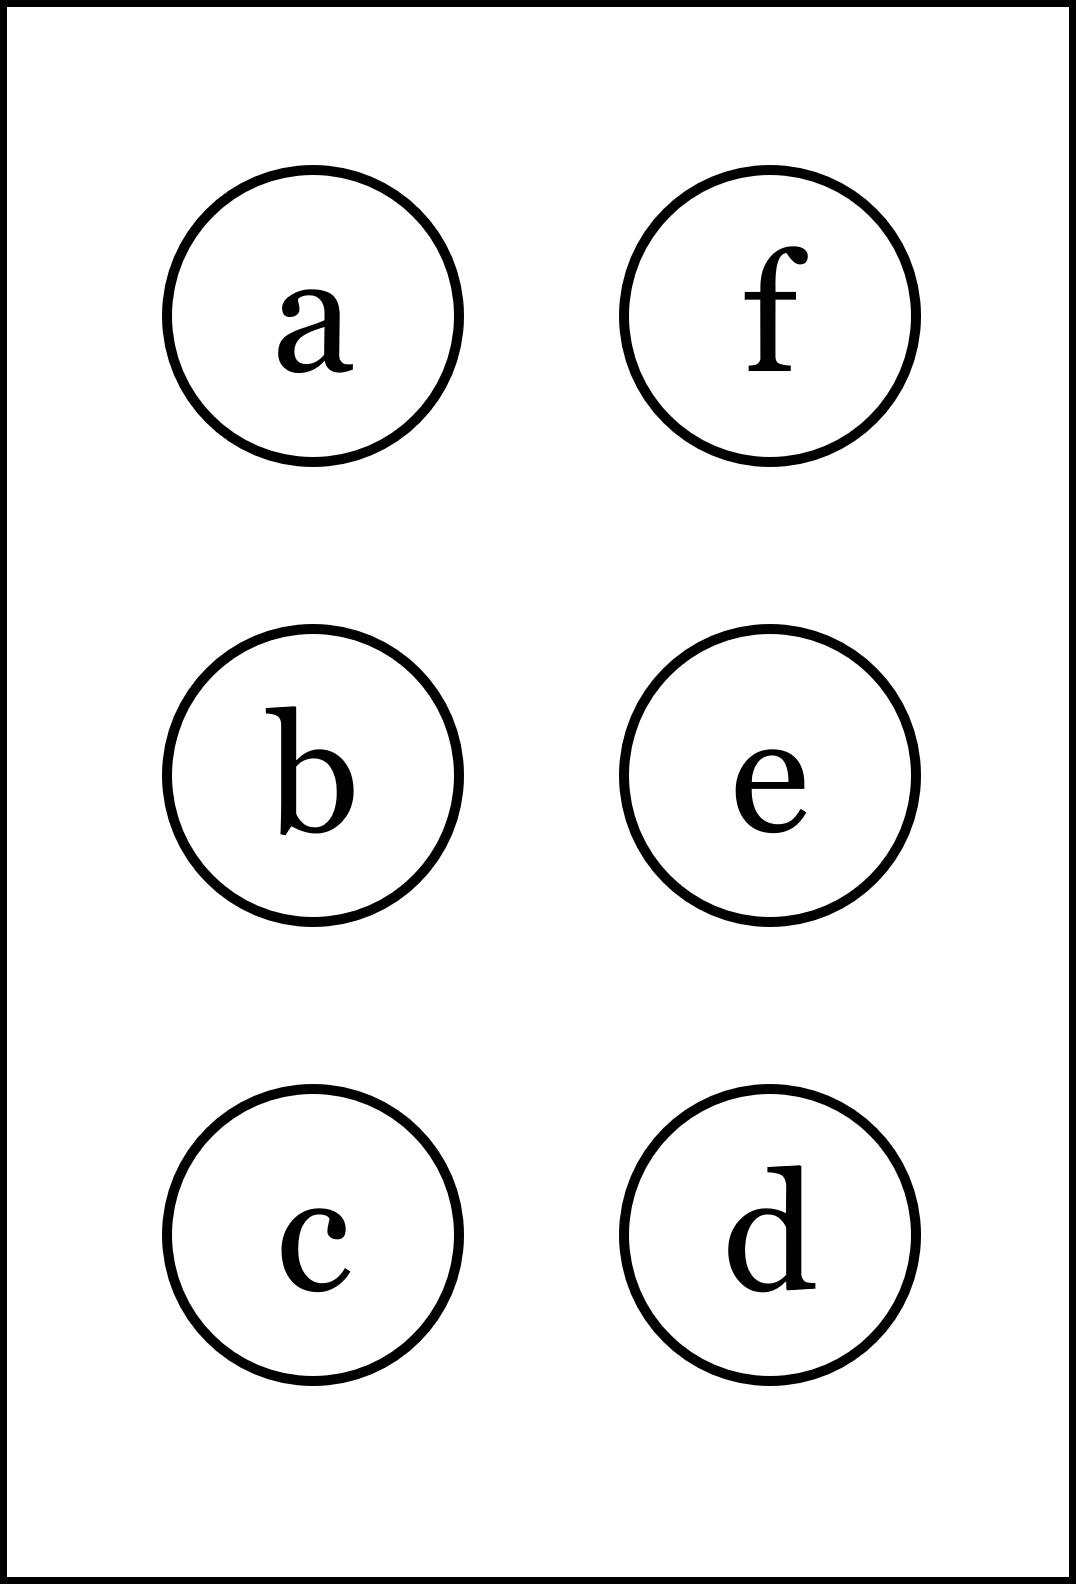
\includegraphics[height=40mm]{../images/braille.png}
{\small Písmeno Braillovej abecedy}
\end{center}
\end{minipage}
\end{center}
\end{minipage}
\\ \hdashline
\begin{minipage}[c][99mm][t]{0.49\linewidth}
\begin{center}
\vspace{7mm}
{\huge Definiční obor, skupina \textit{Delta $\delta$} -\romannumeral3}\\[4.5mm]
\textit{Meno:}\phantom{xxxxxxxxxxxxxxxxxxxxxxxxxxxxxxxxxxxxxxxxxxxxxxxxxxxxxxxxxxxxxxxxx}\\[3.5mm]
\textbf{Zjisti definiční obor} zadaných funkcí. Pokud se shoduje s tím za otazníky,\\tak napravo obarvi příslušející kroužek načerno. \textbf{Spolu odevzdejte výsledné slovo}.\\[3mm]
\begin{minipage}{0.77\linewidth}
\begin{center}
\begin{varwidth}{\textwidth}
\begin{enumerate}
\normalsize
\item $f(x)=\cfrac{-2x-4}{3x-8}$\quad \dotfill\; ???\;\dotfill \quad $\mathbb{R}\smallsetminus\{\nicefrac{8}{3}\}$
\item $f(x)=\cfrac{1}{2x^3+8x^2+2x-12}$\quad \dotfill\; ???\;\dotfill \quad $\mathbb{R}\smallsetminus\{-4,-2,-1\}$
\item $f(x)=-3\sqrt{6x+4}$\quad \dotfill\; ???\;\dotfill \quad $x\geq\nicefrac{-2}{3}$
\item $f(x)=\sqrt{-x^2+3x}$\quad \dotfill\; ???\;\dotfill \quad $x\in(0 , 3)$
\item $f(x)=3\ln{(-7x-5)}$\quad \dotfill\; ???\;\dotfill \quad $x<\nicefrac{-5}{7}$
\item $f(x)=\ln{(x^2-4)}$\quad \dotfill\; ???\;\dotfill \quad $x\in(-\infty , -2)\cup(2 , \infty)$
\end{enumerate}
\end{varwidth}
\end{center}
\end{minipage}
\begin{minipage}{0.20\linewidth}
\begin{center}
{\Huge\bfseries 3.} \\[2mm]
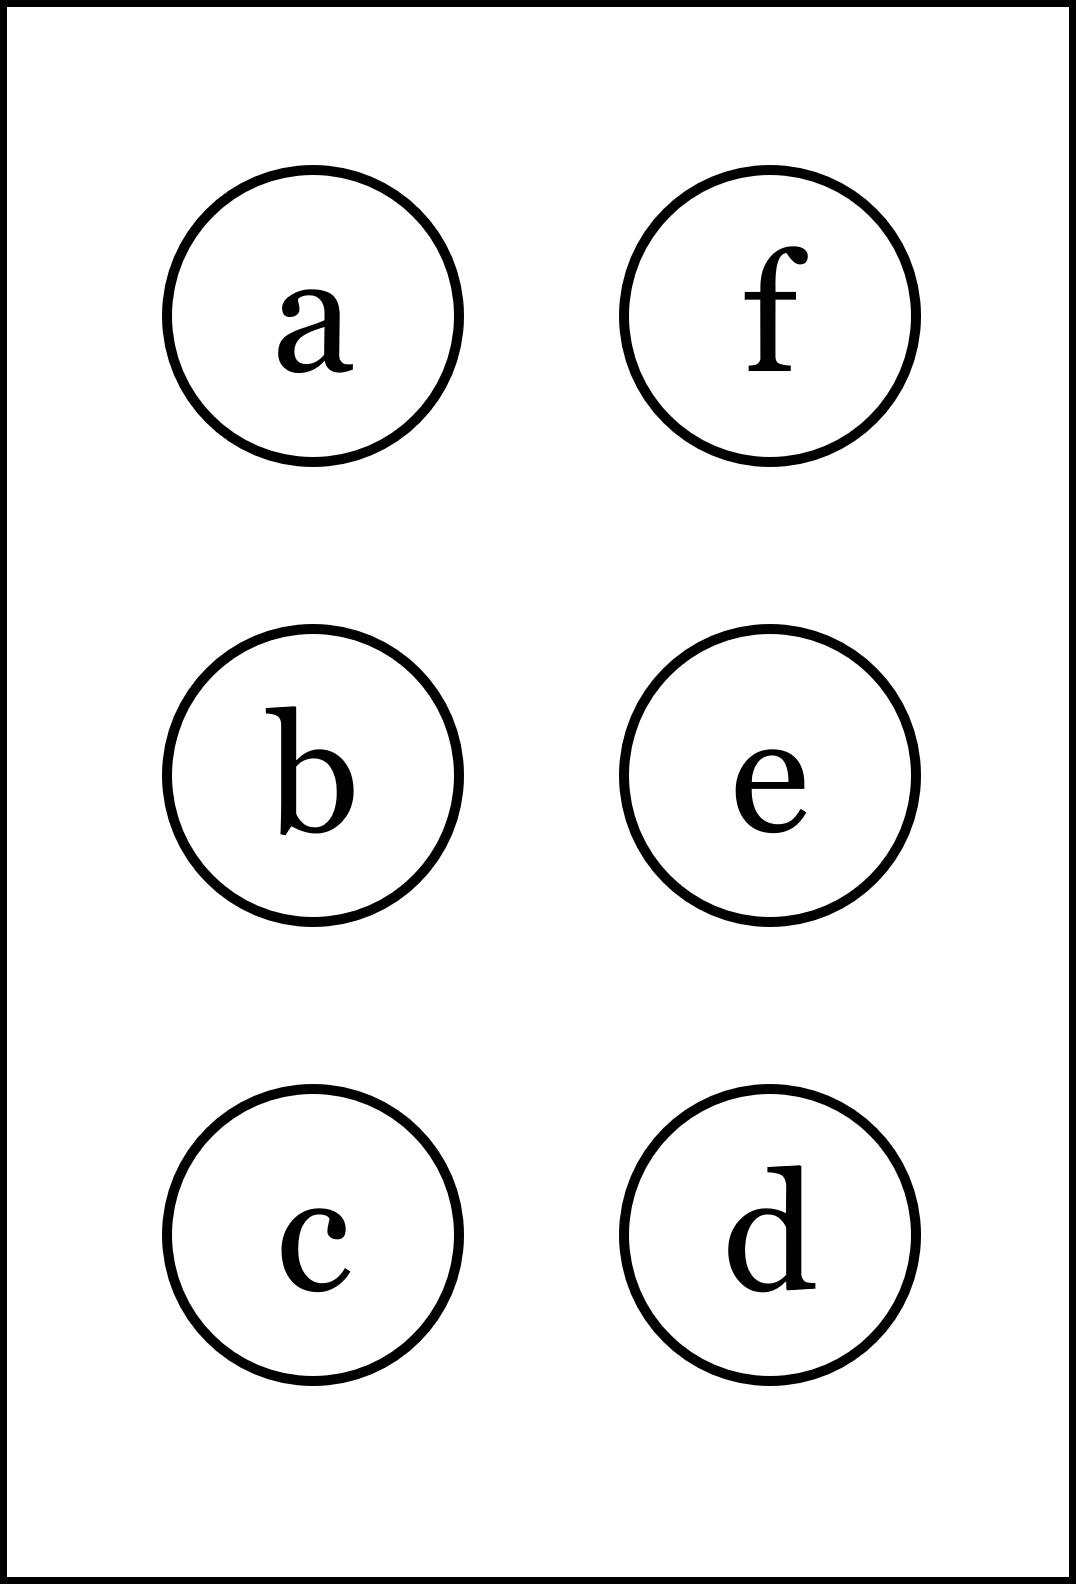
\includegraphics[height=40mm]{../images/braille.png}
{\small Písmeno Braillovej abecedy}
\end{center}
\end{minipage}
\end{center}
\end{minipage}
&
\begin{minipage}[c][99mm][t]{0.49\linewidth}
\begin{center}
\vspace{7mm}
{\huge Definiční obor, skupina \textit{Delta $\delta$} -\romannumeral4}\\[4.5mm]
\textit{Meno:}\phantom{xxxxxxxxxxxxxxxxxxxxxxxxxxxxxxxxxxxxxxxxxxxxxxxxxxxxxxxxxxxxxxxxx}\\[3.5mm]
\textbf{Zjisti definiční obor} zadaných funkcí. Pokud se shoduje s tím za otazníky,\\tak napravo obarvi příslušející kroužek načerno. \textbf{Spolu odevzdejte výsledné slovo}.\\[3mm]
\begin{minipage}{0.77\linewidth}
\begin{center}
\begin{varwidth}{\textwidth}
\begin{enumerate}
\normalsize
\item $f(x)=\cfrac{-5x-7}{2x-1}$\quad \dotfill\; ???\;\dotfill \quad $\mathbb{R}\smallsetminus\{\nicefrac{1}{2}\}$
\item $f(x)=\cfrac{1}{-x^3-2x^2+5x+6}$\quad \dotfill\; ???\;\dotfill \quad $\mathbb{R}\smallsetminus\{1,3,-3\}$
\item $f(x)=2\sqrt{-3x+7}$\quad \dotfill\; ???\;\dotfill \quad $x\geq\nicefrac{7}{3}$
\item $f(x)=\sqrt{-x^2+3x}$\quad \dotfill\; ???\;\dotfill \quad $x\in\langle-3 , 0\rangle$
\item $f(x)=4\ln{(-5x-7)}$\quad \dotfill\; ???\;\dotfill \quad $x<\nicefrac{7}{5}$
\item $f(x)=\ln{(x^2-13x+40)}$\quad \dotfill\; ???\;\dotfill \quad $x\in(5 , 8)$
\end{enumerate}
\end{varwidth}
\end{center}
\end{minipage}
\begin{minipage}{0.20\linewidth}
\begin{center}
{\Huge\bfseries 4.} \\[2mm]
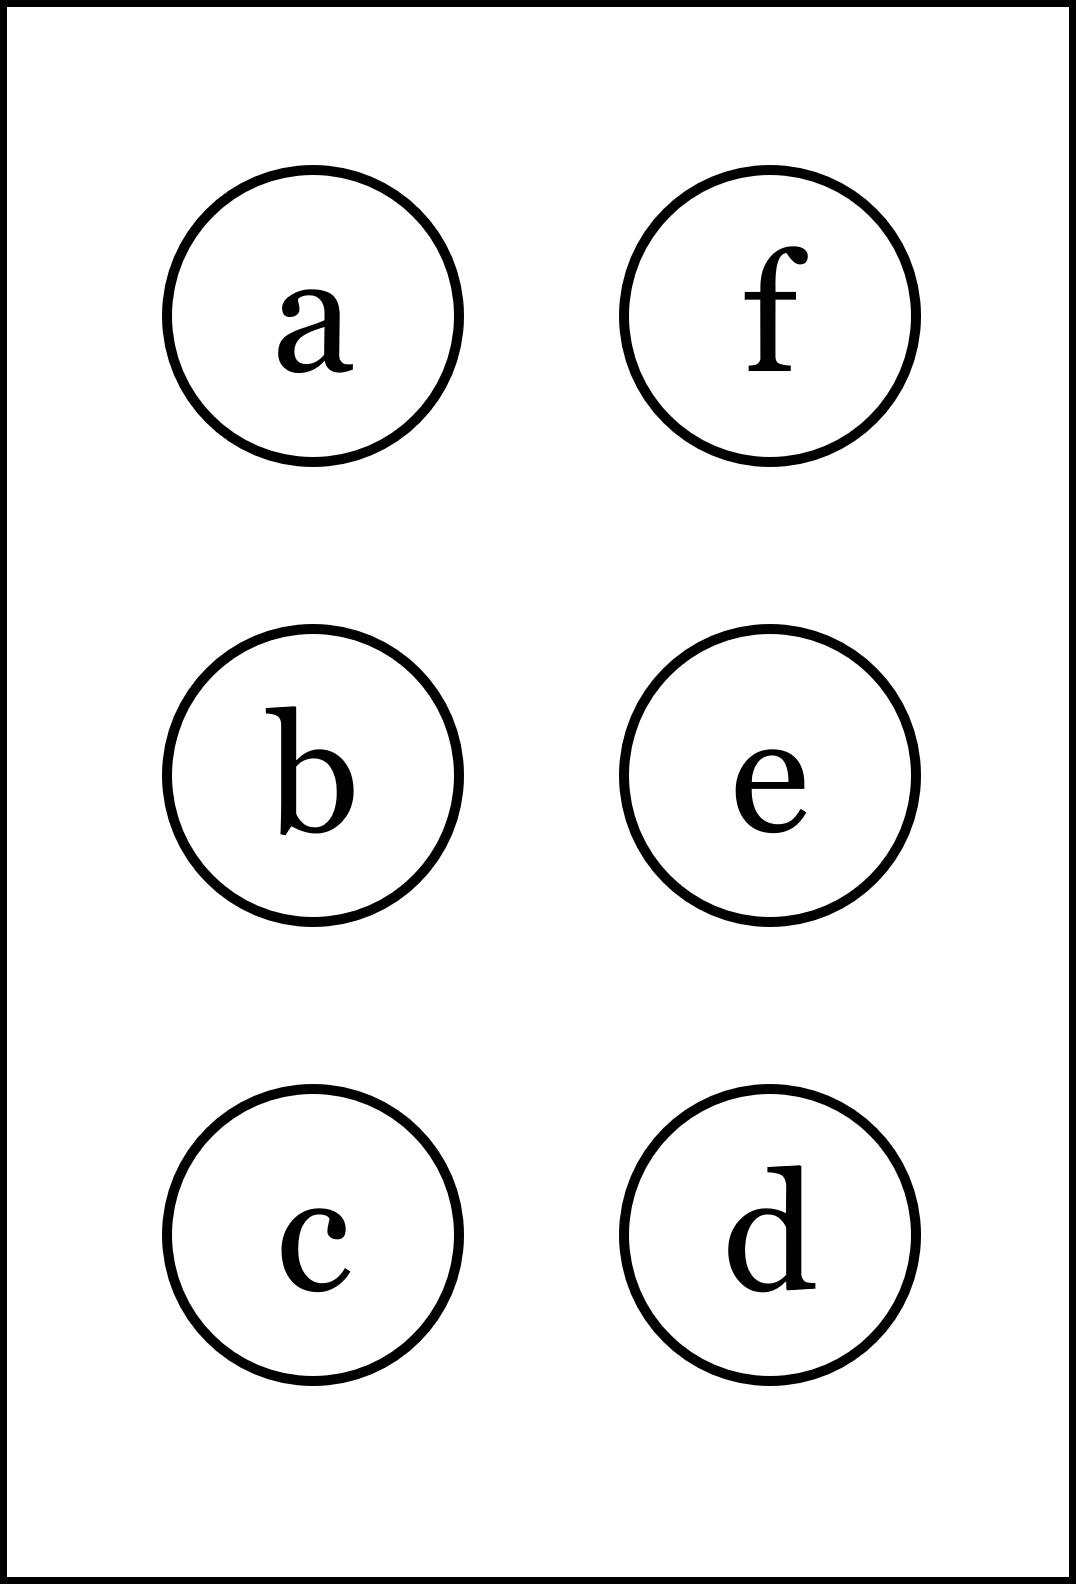
\includegraphics[height=40mm]{../images/braille.png}
{\small Písmeno Braillovej abecedy}
\end{center}
\end{minipage}
\end{center}
\end{minipage}
%
\end{tabular}
\begin{tikzpicture}[remember picture,overlay]\node[xshift=7mm,yshift=-100.6mm,anchor=north west] at (current page.north west){\ding{33}};\end{tikzpicture}
\begin{tikzpicture}[remember picture,overlay]\node[xshift=151.2mm,yshift=-7mm,anchor=north west,rotate=270] at (current page.north west){\ding{33}};\end{tikzpicture}
\newpage
\thispagestyle{empty}
\begin{tabular}{c:c}
\begin{minipage}[c][99mm][t]{0.49\linewidth}
\begin{center}
\vspace{7mm}
{\huge Definiční obor, skupina \textit{Epsilon $\epsilon$} -\romannumeral1}\\[4.5mm]
\textit{Meno:}\phantom{xxxxxxxxxxxxxxxxxxxxxxxxxxxxxxxxxxxxxxxxxxxxxxxxxxxxxxxxxxxxxxxxx}\\[3.5mm]
\textbf{Zjisti definiční obor} zadaných funkcí. Pokud se shoduje s tím za otazníky,\\tak napravo obarvi příslušející kroužek načerno. \textbf{Spolu odevzdejte výsledné slovo}.\\[3mm]
\begin{minipage}{0.77\linewidth}
\begin{center}
\begin{varwidth}{\textwidth}
\begin{enumerate}
\normalsize
\item $f(x)=\cfrac{-x+4}{-2x-3}$\quad \dotfill\; ???\;\dotfill \quad $\mathbb{R}\smallsetminus\{\nicefrac{-3}{2}\}$
\item $f(x)=\cfrac{1}{4x^3+16x^2-44x+24}$\quad \dotfill\; ???\;\dotfill \quad $\mathbb{R}\smallsetminus\{1,-6\}$
\item $f(x)=-2\sqrt{-3x+3}$\quad \dotfill\; ???\;\dotfill \quad $x\leq1$
\item $f(x)=\sqrt{-x^2+4x}$\quad \dotfill\; ???\;\dotfill \quad $x\in(0 , 4)$
\item $f(x)=-4\ln{(3x-1)}$\quad \dotfill\; ???\;\dotfill \quad $x>\nicefrac{1}{3}$
\item $f(x)=\ln{(x^2-3x+2)}$\quad \dotfill\; ???\;\dotfill \quad $x\in(1 , 2)$
\end{enumerate}
\end{varwidth}
\end{center}
\end{minipage}
\begin{minipage}{0.20\linewidth}
\begin{center}
{\Huge\bfseries 1.} \\[2mm]
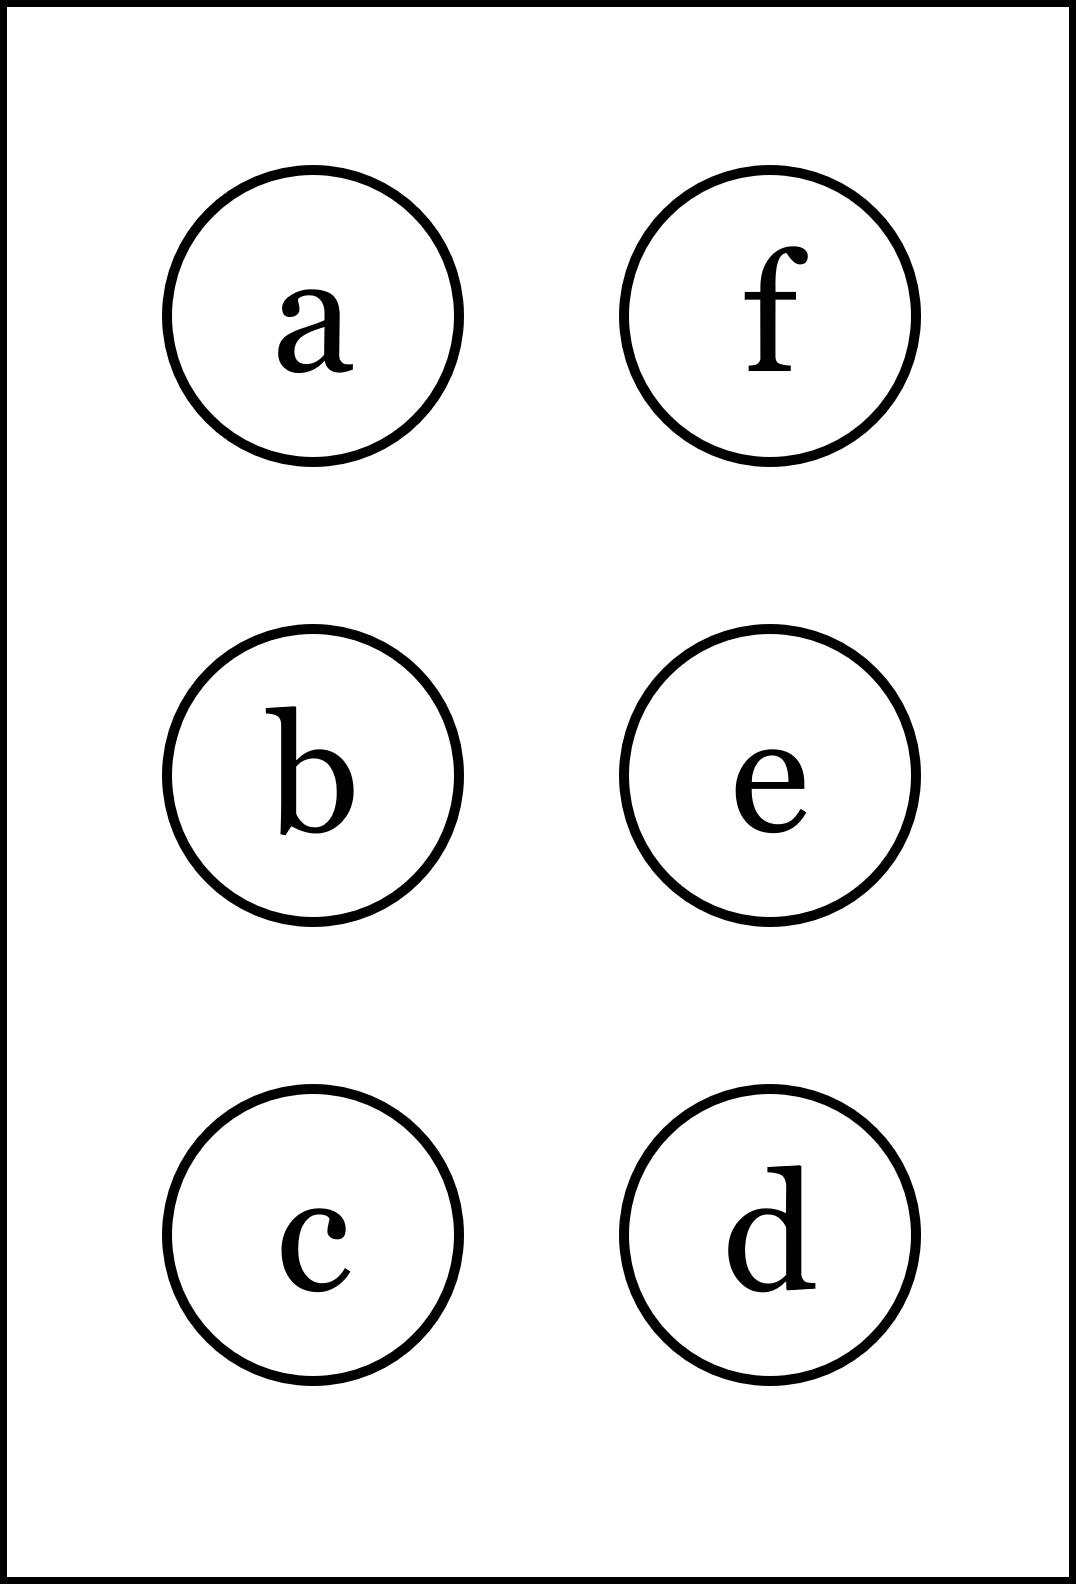
\includegraphics[height=40mm]{../images/braille.png}
{\small Písmeno Braillovej abecedy}
\end{center}
\end{minipage}
\end{center}
\end{minipage}
&
\begin{minipage}[c][99mm][t]{0.49\linewidth}
\begin{center}
\vspace{7mm}
{\huge Definiční obor, skupina \textit{Epsilon $\epsilon$} -\romannumeral2}\\[4.5mm]
\textit{Meno:}\phantom{xxxxxxxxxxxxxxxxxxxxxxxxxxxxxxxxxxxxxxxxxxxxxxxxxxxxxxxxxxxxxxxxx}\\[3.5mm]
\textbf{Zjisti definiční obor} zadaných funkcí. Pokud se shoduje s tím za otazníky,\\tak napravo obarvi příslušející kroužek načerno. \textbf{Spolu odevzdejte výsledné slovo}.\\[3mm]
\begin{minipage}{0.77\linewidth}
\begin{center}
\begin{varwidth}{\textwidth}
\begin{enumerate}
\normalsize
\item $f(x)=\cfrac{-5x-3}{5x-1}$\quad \dotfill\; ???\;\dotfill \quad $\mathbb{R}\smallsetminus\{\nicefrac{1}{5}\}$
\item $f(x)=\cfrac{1}{-x^3-4x^2+x+4}$\quad \dotfill\; ???\;\dotfill \quad $\mathbb{R}\smallsetminus\{2,4,-1\}$
\item $f(x)=1\sqrt{-2x-1}$\quad \dotfill\; ???\;\dotfill \quad $x\leq\nicefrac{1}{2}$
\item $f(x)=\sqrt{-x^2+5x}$\quad \dotfill\; ???\;\dotfill \quad $x\in\langle-5 , 0\rangle$
\item $f(x)=3\ln{(4x+2)}$\quad \dotfill\; ???\;\dotfill \quad $x>\nicefrac{-1}{2}$
\item $f(x)=\ln{(x^2+3x-18)}$\quad \dotfill\; ???\;\dotfill \quad $x\in(-6 , 3)$
\end{enumerate}
\end{varwidth}
\end{center}
\end{minipage}
\begin{minipage}{0.20\linewidth}
\begin{center}
{\Huge\bfseries 2.} \\[2mm]
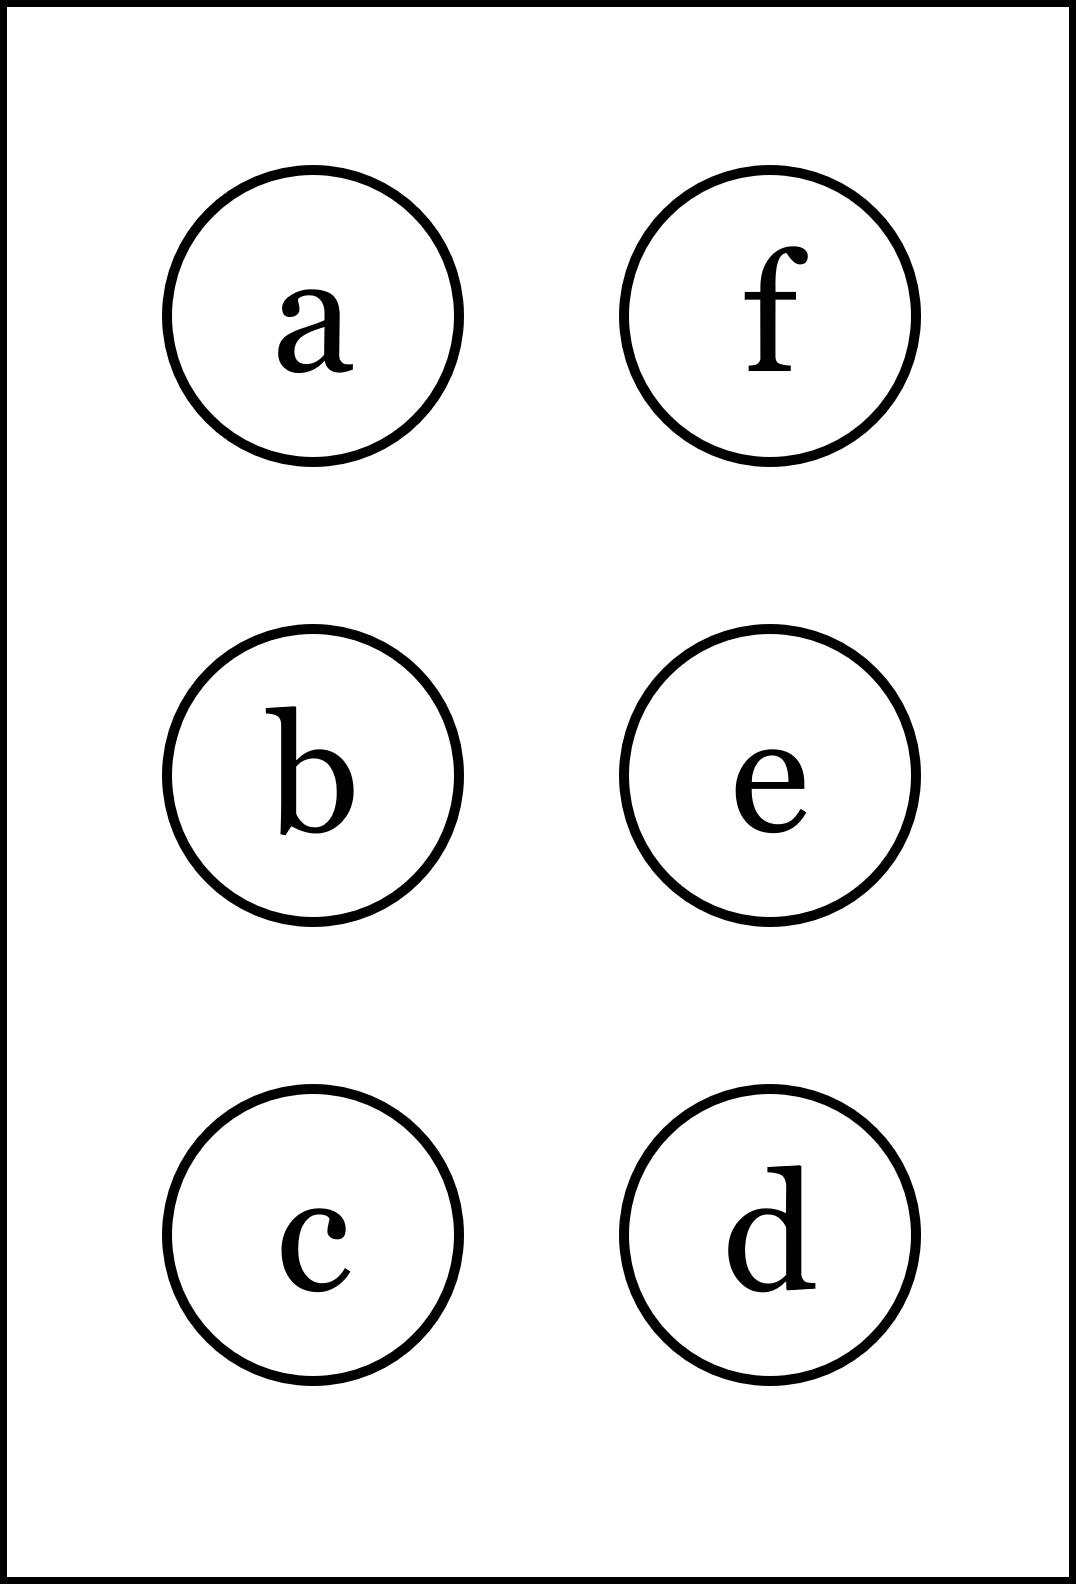
\includegraphics[height=40mm]{../images/braille.png}
{\small Písmeno Braillovej abecedy}
\end{center}
\end{minipage}
\end{center}
\end{minipage}
\\ \hdashline
\begin{minipage}[c][99mm][t]{0.49\linewidth}
\begin{center}
\vspace{7mm}
{\huge Definiční obor, skupina \textit{Epsilon $\epsilon$} -\romannumeral3}\\[4.5mm]
\textit{Meno:}\phantom{xxxxxxxxxxxxxxxxxxxxxxxxxxxxxxxxxxxxxxxxxxxxxxxxxxxxxxxxxxxxxxxxx}\\[3.5mm]
\textbf{Zjisti definiční obor} zadaných funkcí. Pokud se shoduje s tím za otazníky,\\tak napravo obarvi příslušející kroužek načerno. \textbf{Spolu odevzdejte výsledné slovo}.\\[3mm]
\begin{minipage}{0.77\linewidth}
\begin{center}
\begin{varwidth}{\textwidth}
\begin{enumerate}
\normalsize
\item $f(x)=\cfrac{-x+8}{-2x+3}$\quad \dotfill\; ???\;\dotfill \quad $\mathbb{R}\smallsetminus\{\nicefrac{3}{2}\}$
\item $f(x)=\cfrac{1}{-x^3-13x^2-39x-27}$\quad \dotfill\; ???\;\dotfill \quad $\mathbb{R}\smallsetminus\{-3,-1,-9\}$
\item $f(x)=6\sqrt{-x+5}$\quad \dotfill\; ???\;\dotfill \quad $x\leq5$
\item $f(x)=\sqrt{-x^2+4x}$\quad \dotfill\; ???\;\dotfill \quad $x\in\langle-4 , 0\rangle$
\item $f(x)=-1\ln{(2x+3)}$\quad \dotfill\; ???\;\dotfill \quad $x>\nicefrac{3}{2}$
\item $f(x)=\ln{(x^2-3x-28)}$\quad \dotfill\; ???\;\dotfill \quad $x\in(-\infty , -4)\cup(7 , \infty)$
\end{enumerate}
\end{varwidth}
\end{center}
\end{minipage}
\begin{minipage}{0.20\linewidth}
\begin{center}
{\Huge\bfseries 3.} \\[2mm]
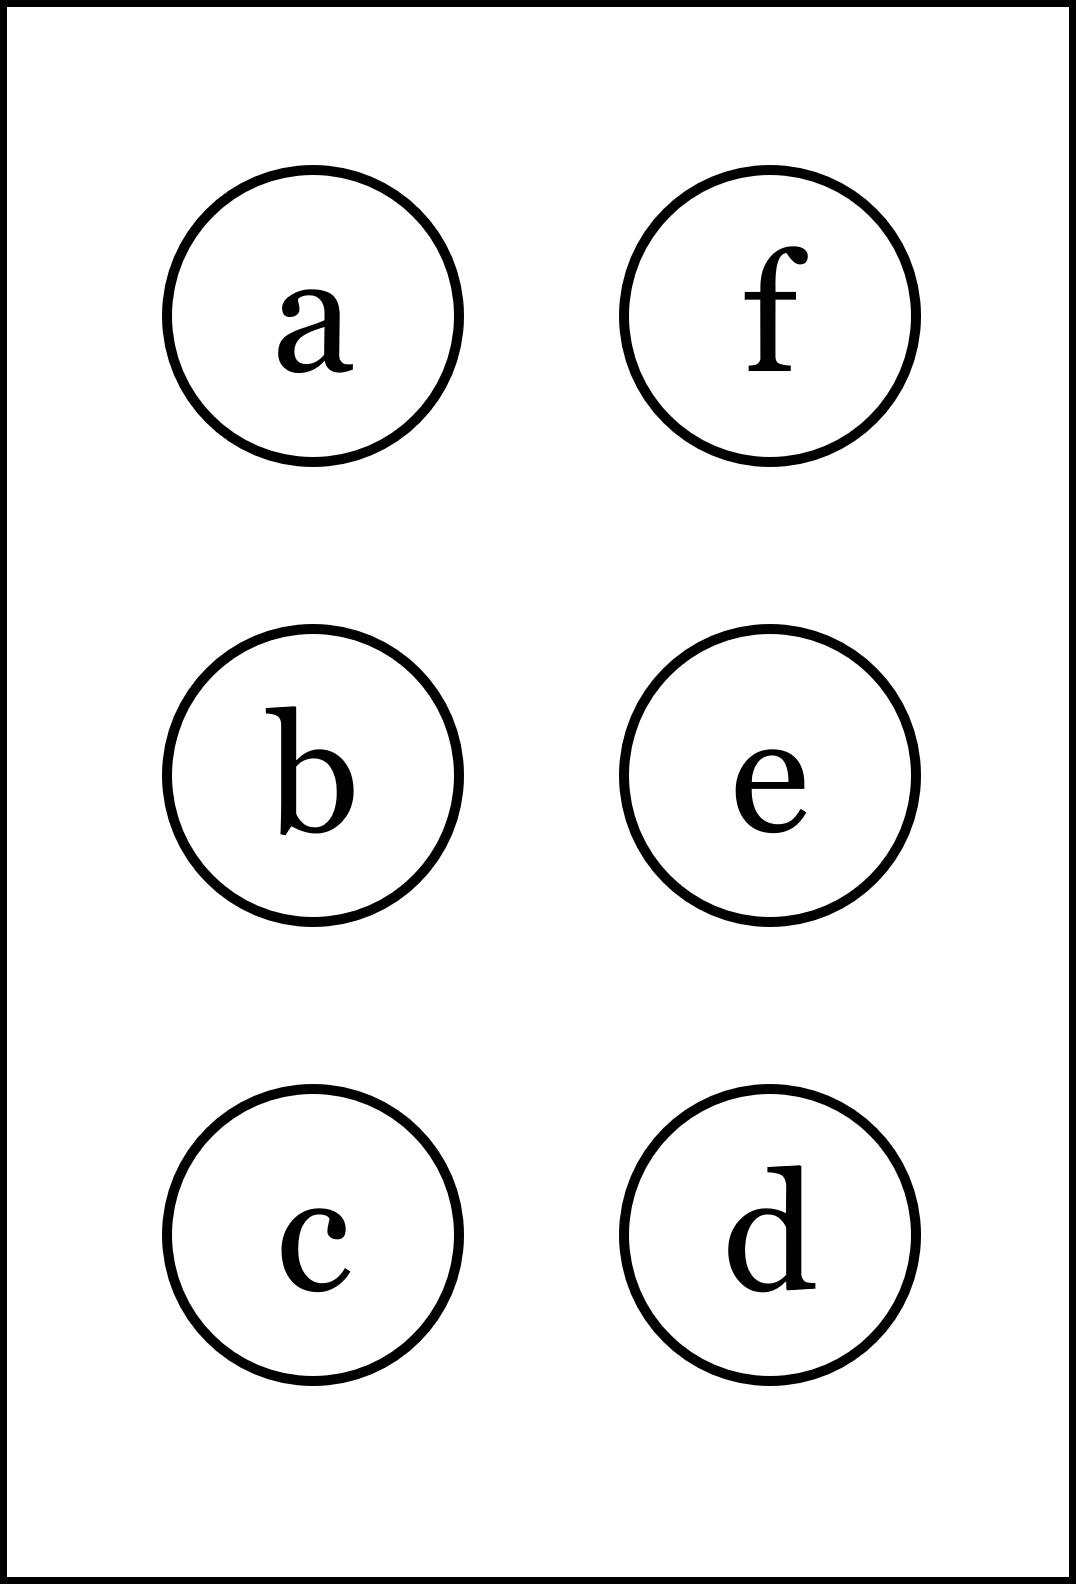
\includegraphics[height=40mm]{../images/braille.png}
{\small Písmeno Braillovej abecedy}
\end{center}
\end{minipage}
\end{center}
\end{minipage}
&
\begin{minipage}[c][99mm][t]{0.49\linewidth}
\begin{center}
\vspace{7mm}
{\huge Definiční obor, skupina \textit{Epsilon $\epsilon$} -\romannumeral4}\\[4.5mm]
\textit{Meno:}\phantom{xxxxxxxxxxxxxxxxxxxxxxxxxxxxxxxxxxxxxxxxxxxxxxxxxxxxxxxxxxxxxxxxx}\\[3.5mm]
\textbf{Zjisti definiční obor} zadaných funkcí. Pokud se shoduje s tím za otazníky,\\tak napravo obarvi příslušející kroužek načerno. \textbf{Spolu odevzdejte výsledné slovo}.\\[3mm]
\begin{minipage}{0.77\linewidth}
\begin{center}
\begin{varwidth}{\textwidth}
\begin{enumerate}
\normalsize
\item $f(x)=\cfrac{2x-2}{-5x-5}$\quad \dotfill\; ???\;\dotfill \quad $\mathbb{R}\smallsetminus\{-1\}$
\item $f(x)=\cfrac{1}{6x^3-12x^2-30x+36}$\quad \dotfill\; ???\;\dotfill \quad $\mathbb{R}\smallsetminus\{3,-3,-1\}$
\item $f(x)=1\sqrt{3x+2}$\quad \dotfill\; ???\;\dotfill \quad $x\geq\nicefrac{2}{3}$
\item $f(x)=\sqrt{-x^2-7x}$\quad \dotfill\; ???\;\dotfill \quad $x\in(-7 , 0)$
\item $f(x)=-2\ln{(9x-1)}$\quad \dotfill\; ???\;\dotfill \quad $x<\nicefrac{1}{9}$
\item $f(x)=\ln{(x^2+5x-6)}$\quad \dotfill\; ???\;\dotfill \quad $x\in(-6 , 1)$
\end{enumerate}
\end{varwidth}
\end{center}
\end{minipage}
\begin{minipage}{0.20\linewidth}
\begin{center}
{\Huge\bfseries 4.} \\[2mm]
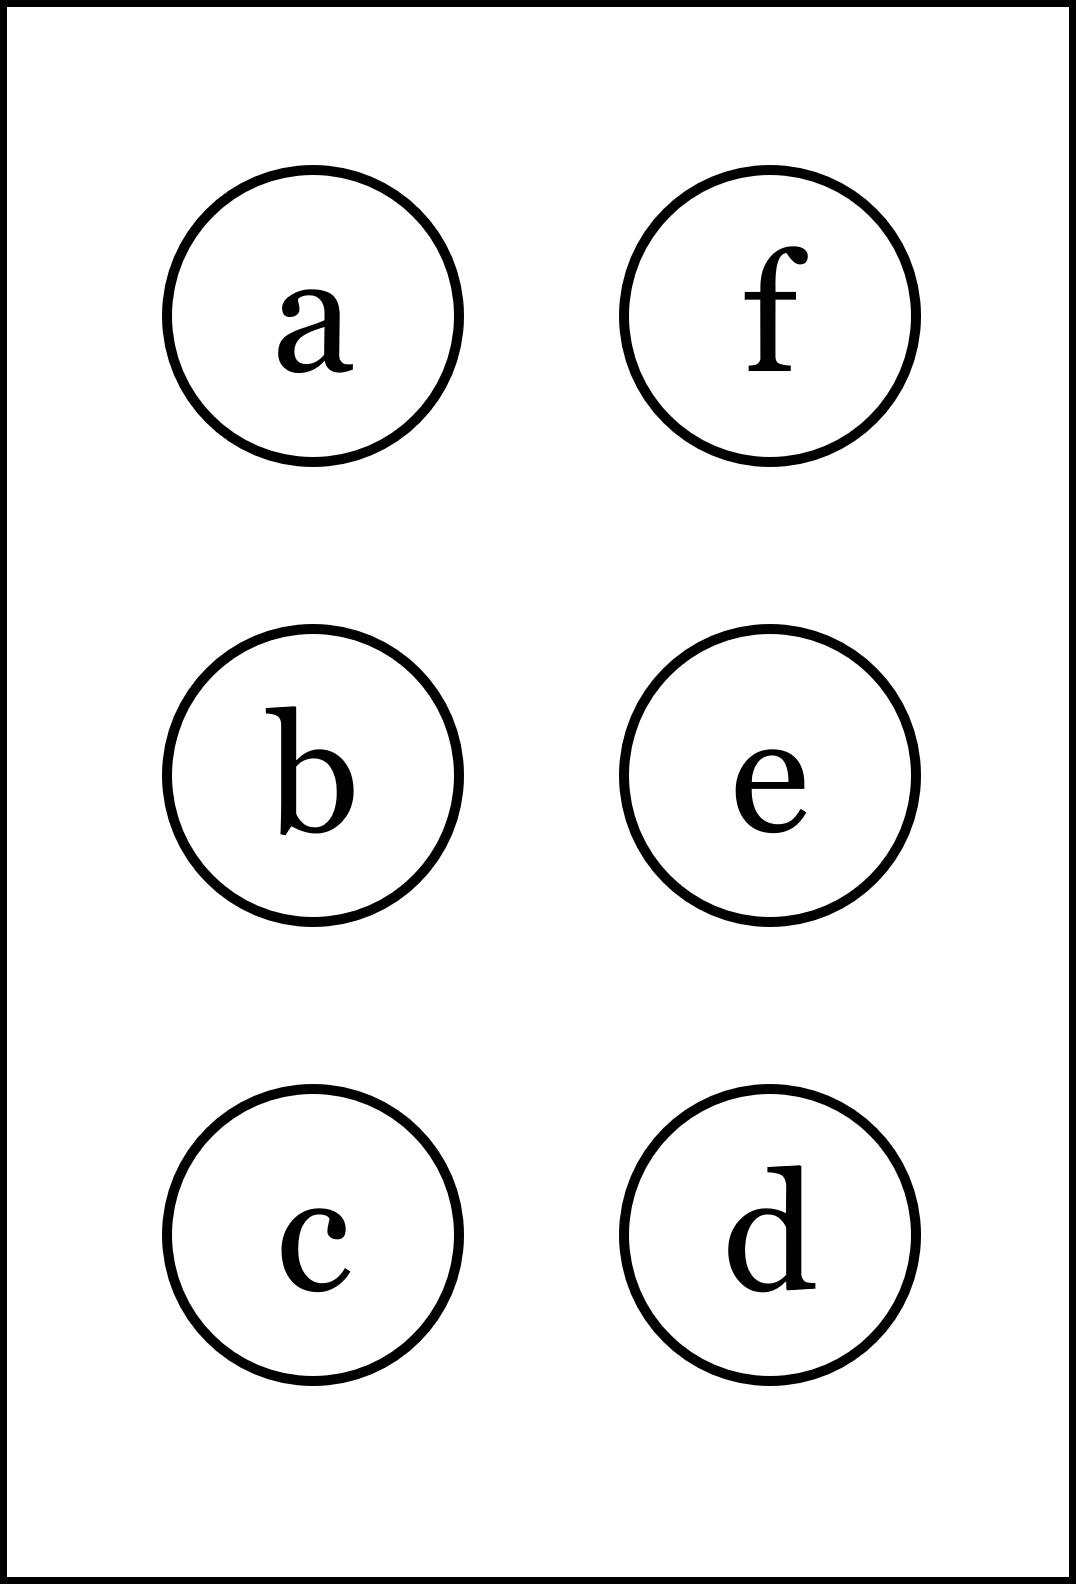
\includegraphics[height=40mm]{../images/braille.png}
{\small Písmeno Braillovej abecedy}
\end{center}
\end{minipage}
\end{center}
\end{minipage}
%
\end{tabular}
\begin{tikzpicture}[remember picture,overlay]\node[xshift=7mm,yshift=-100.6mm,anchor=north west] at (current page.north west){\ding{33}};\end{tikzpicture}
\begin{tikzpicture}[remember picture,overlay]\node[xshift=151.2mm,yshift=-7mm,anchor=north west,rotate=270] at (current page.north west){\ding{33}};\end{tikzpicture}
\newpage
\thispagestyle{empty}
\begin{tabular}{c:c}
\begin{minipage}[c][99mm][t]{0.49\linewidth}
\begin{center}
\vspace{7mm}
{\huge Definiční obor, skupina \textit{Zeta $\zeta$} -\romannumeral1}\\[4.5mm]
\textit{Meno:}\phantom{xxxxxxxxxxxxxxxxxxxxxxxxxxxxxxxxxxxxxxxxxxxxxxxxxxxxxxxxxxxxxxxxx}\\[3.5mm]
\textbf{Zjisti definiční obor} zadaných funkcí. Pokud se shoduje s tím za otazníky,\\tak napravo obarvi příslušející kroužek načerno. \textbf{Spolu odevzdejte výsledné slovo}.\\[3mm]
\begin{minipage}{0.77\linewidth}
\begin{center}
\begin{varwidth}{\textwidth}
\begin{enumerate}
\normalsize
\item $f(x)=\cfrac{3x-3}{9x+6}$\quad \dotfill\; ???\;\dotfill \quad $\mathbb{R}\smallsetminus\{\nicefrac{-2}{3}\}$
\item $f(x)=\cfrac{1}{x^3+x^2-22x-40}$\quad \dotfill\; ???\;\dotfill \quad $\mathbb{R}\smallsetminus\{-4,5,-2\}$
\item $f(x)=-7\sqrt{-7x-1}$\quad \dotfill\; ???\;\dotfill \quad $x\leq\nicefrac{-1}{7}$
\item $f(x)=\sqrt{-x^2+6x}$\quad \dotfill\; ???\;\dotfill \quad $x\in\langle-6 , 0\rangle$
\item $f(x)=-4\ln{(2x-6)}$\quad \dotfill\; ???\;\dotfill \quad $x>-3$
\item $f(x)=\ln{(x^2-3x-4)}$\quad \dotfill\; ???\;\dotfill \quad $x\in(-1 , 4)$
\end{enumerate}
\end{varwidth}
\end{center}
\end{minipage}
\begin{minipage}{0.20\linewidth}
\begin{center}
{\Huge\bfseries 1.} \\[2mm]
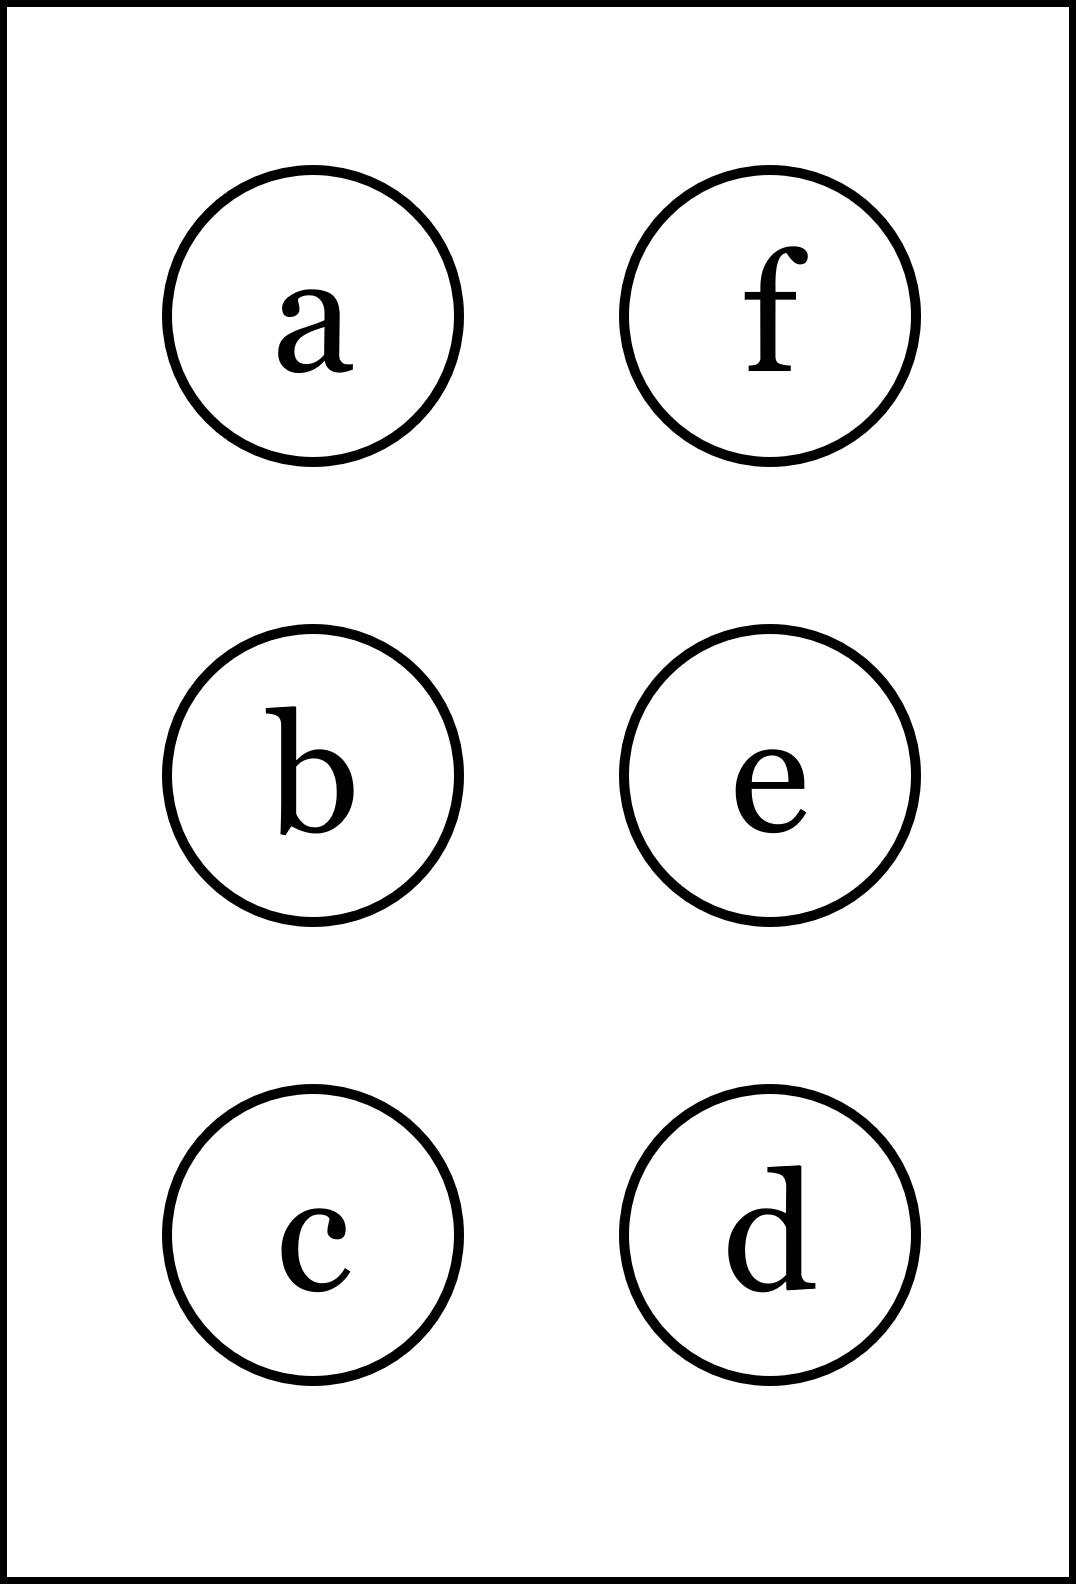
\includegraphics[height=40mm]{../images/braille.png}
{\small Písmeno Braillovej abecedy}
\end{center}
\end{minipage}
\end{center}
\end{minipage}
&
\begin{minipage}[c][99mm][t]{0.49\linewidth}
\begin{center}
\vspace{7mm}
{\huge Definiční obor, skupina \textit{Zeta $\zeta$} -\romannumeral2}\\[4.5mm]
\textit{Meno:}\phantom{xxxxxxxxxxxxxxxxxxxxxxxxxxxxxxxxxxxxxxxxxxxxxxxxxxxxxxxxxxxxxxxxx}\\[3.5mm]
\textbf{Zjisti definiční obor} zadaných funkcí. Pokud se shoduje s tím za otazníky,\\tak napravo obarvi příslušející kroužek načerno. \textbf{Spolu odevzdejte výsledné slovo}.\\[3mm]
\begin{minipage}{0.77\linewidth}
\begin{center}
\begin{varwidth}{\textwidth}
\begin{enumerate}
\normalsize
\item $f(x)=\cfrac{-4x-5}{-2x+4}$\quad \dotfill\; ???\;\dotfill \quad $\mathbb{R}\smallsetminus\{2\}$
\item $f(x)=\cfrac{1}{x^3-5x^2+8x-4}$\quad \dotfill\; ???\;\dotfill \quad $\mathbb{R}\smallsetminus\{0,2,-1\}$
\item $f(x)=1\sqrt{-x+5}$\quad \dotfill\; ???\;\dotfill \quad $x\leq-5$
\item $f(x)=\sqrt{-x^2-3x}$\quad \dotfill\; ???\;\dotfill \quad $x\in(-3 , 0)$
\item $f(x)=-3\ln{(3x+3)}$\quad \dotfill\; ???\;\dotfill \quad $x>1$
\item $f(x)=\ln{(x^2-2x-8)}$\quad \dotfill\; ???\;\dotfill \quad $x\in(-2 , 4)$
\end{enumerate}
\end{varwidth}
\end{center}
\end{minipage}
\begin{minipage}{0.20\linewidth}
\begin{center}
{\Huge\bfseries 2.} \\[2mm]
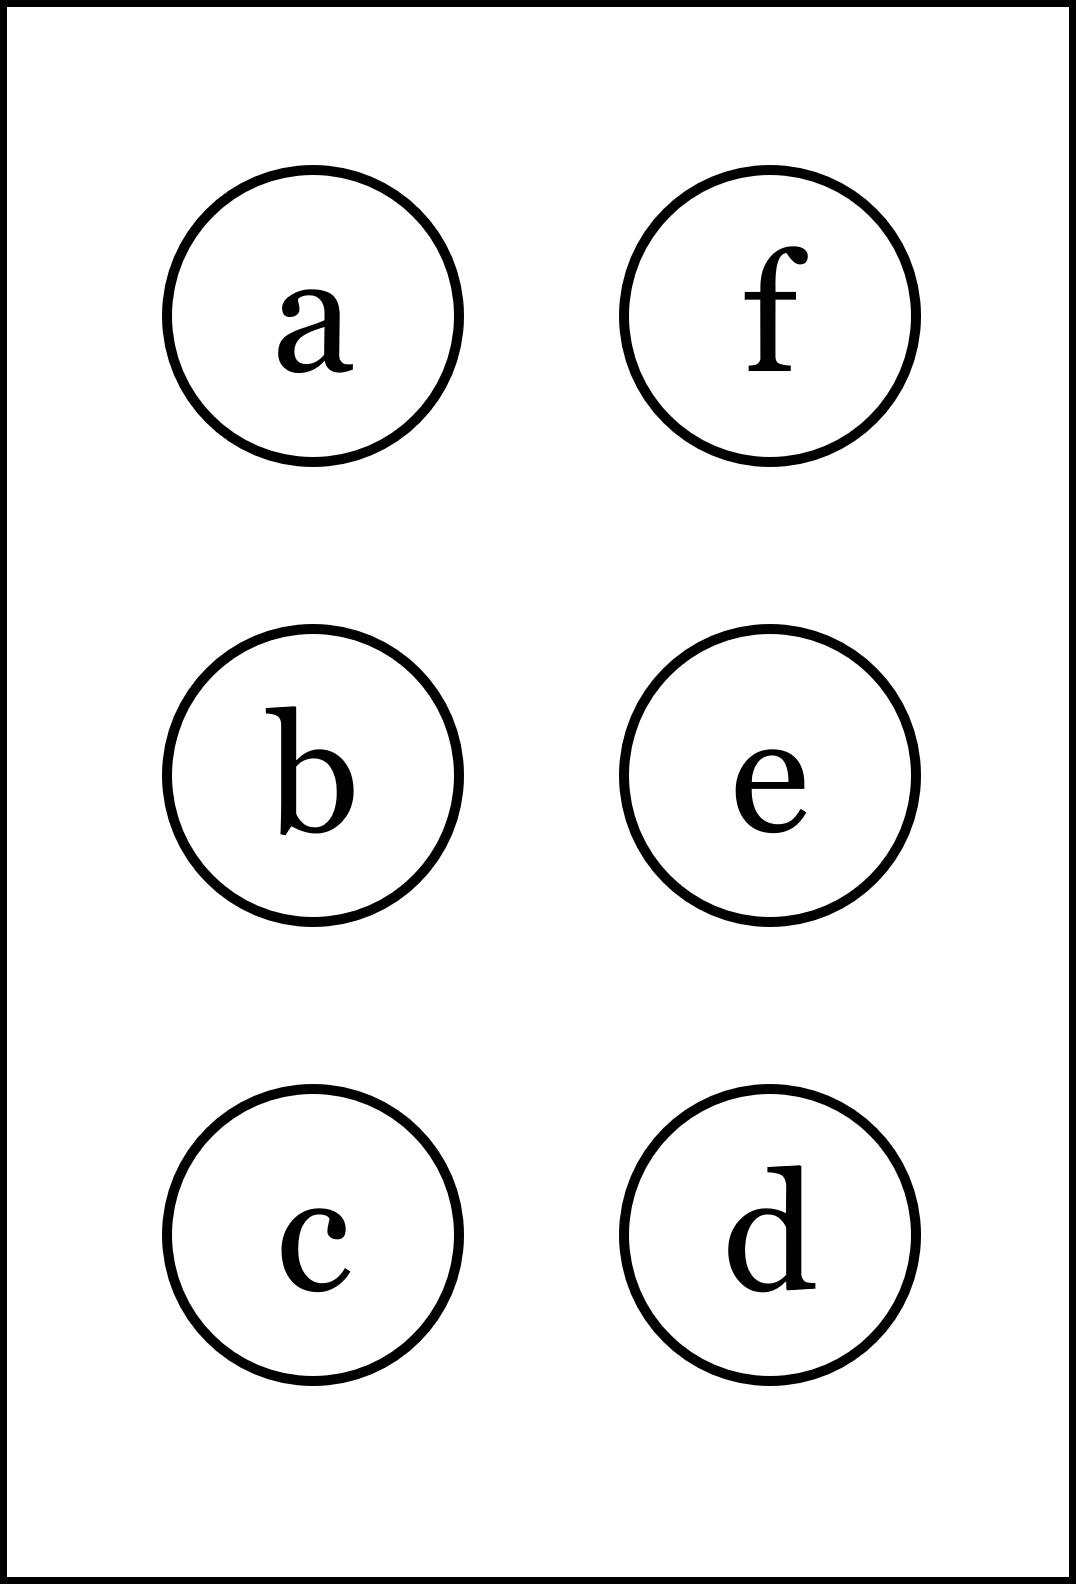
\includegraphics[height=40mm]{../images/braille.png}
{\small Písmeno Braillovej abecedy}
\end{center}
\end{minipage}
\end{center}
\end{minipage}
\\ \hdashline
\begin{minipage}[c][99mm][t]{0.49\linewidth}
\begin{center}
\vspace{7mm}
{\huge Definiční obor, skupina \textit{Zeta $\zeta$} -\romannumeral3}\\[4.5mm]
\textit{Meno:}\phantom{xxxxxxxxxxxxxxxxxxxxxxxxxxxxxxxxxxxxxxxxxxxxxxxxxxxxxxxxxxxxxxxxx}\\[3.5mm]
\textbf{Zjisti definiční obor} zadaných funkcí. Pokud se shoduje s tím za otazníky,\\tak napravo obarvi příslušející kroužek načerno. \textbf{Spolu odevzdejte výsledné slovo}.\\[3mm]
\begin{minipage}{0.77\linewidth}
\begin{center}
\begin{varwidth}{\textwidth}
\begin{enumerate}
\normalsize
\item $f(x)=\cfrac{3x+1}{3x-1}$\quad \dotfill\; ???\;\dotfill \quad $\mathbb{R}\smallsetminus\{\nicefrac{1}{3}\}$
\item $f(x)=\cfrac{1}{-2x^3+10x^2-16x+8}$\quad \dotfill\; ???\;\dotfill \quad $\mathbb{R}\smallsetminus\{1,3,-2\}$
\item $f(x)=5\sqrt{5x-1}$\quad \dotfill\; ???\;\dotfill \quad $x\geq\nicefrac{1}{5}$
\item $f(x)=\sqrt{-x^2+x}$\quad \dotfill\; ???\;\dotfill \quad $x\in\langle-1 , 0\rangle$
\item $f(x)=-4\ln{(-5x+3)}$\quad \dotfill\; ???\;\dotfill \quad $x<\nicefrac{3}{5}$
\item $f(x)=\ln{(x^2-6x+5)}$\quad \dotfill\; ???\;\dotfill \quad $x\in(-\infty , 1)\cup(5 , \infty)$
\end{enumerate}
\end{varwidth}
\end{center}
\end{minipage}
\begin{minipage}{0.20\linewidth}
\begin{center}
{\Huge\bfseries 3.} \\[2mm]
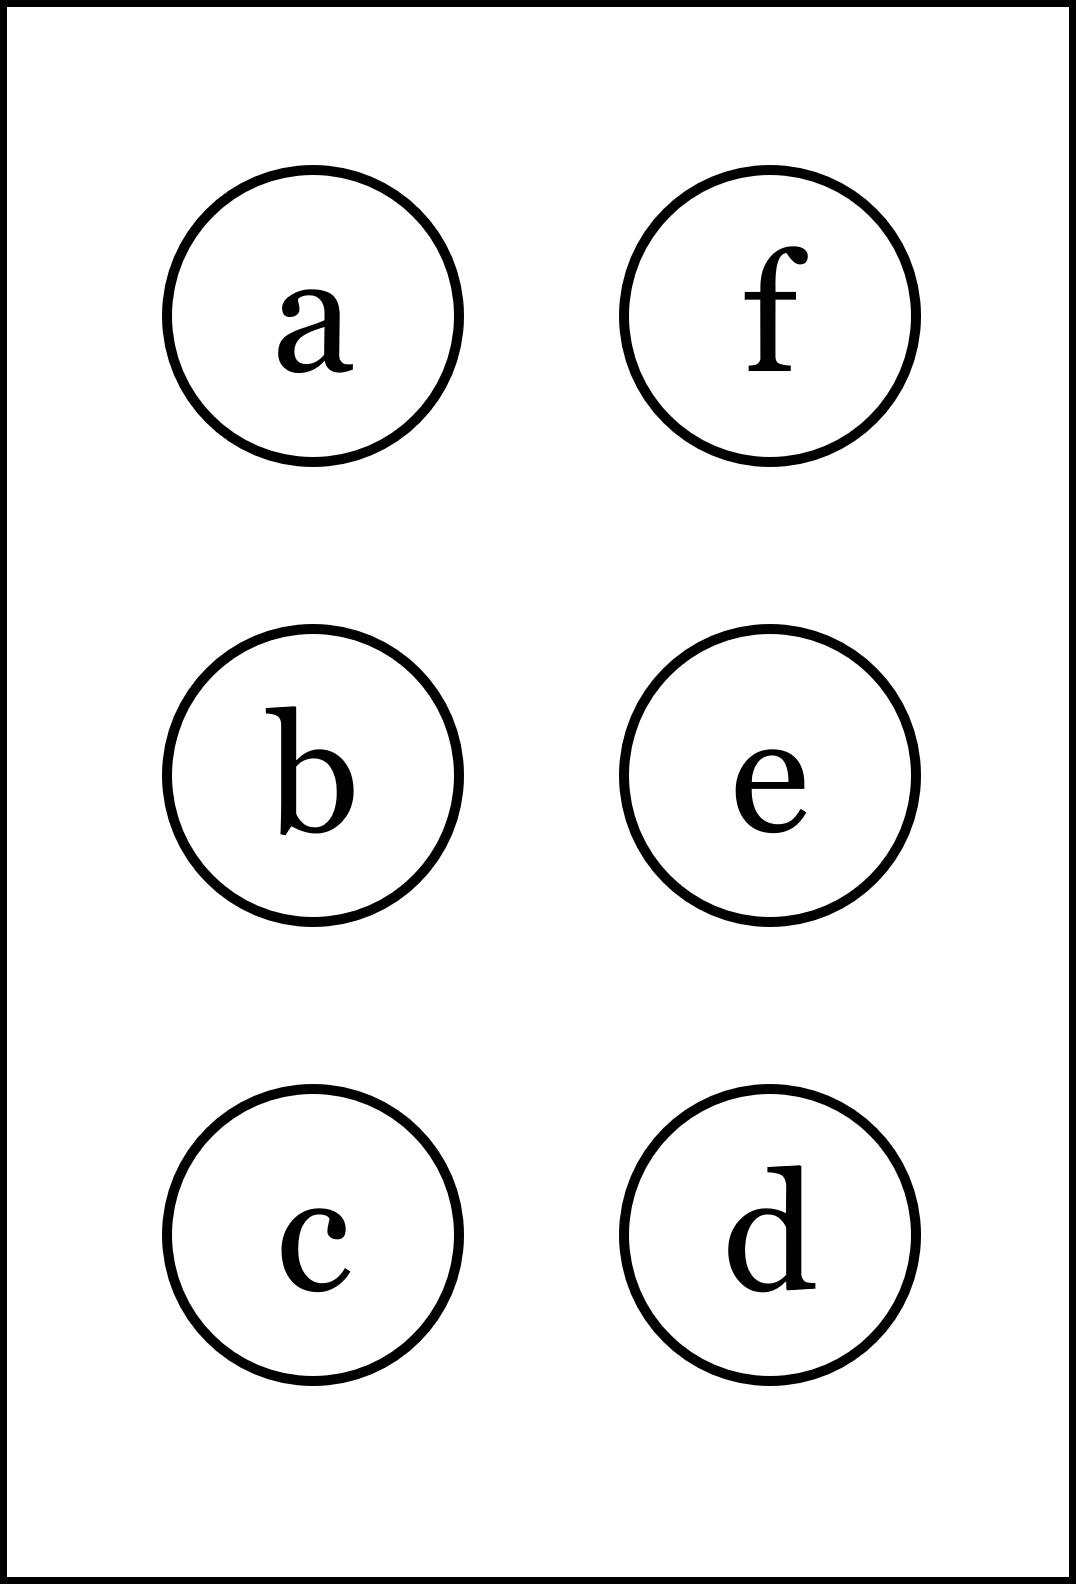
\includegraphics[height=40mm]{../images/braille.png}
{\small Písmeno Braillovej abecedy}
\end{center}
\end{minipage}
\end{center}
\end{minipage}
&
\begin{minipage}[c][99mm][t]{0.49\linewidth}
\begin{center}
\vspace{7mm}
{\huge Definiční obor, skupina \textit{Zeta $\zeta$} -\romannumeral4}\\[4.5mm]
\textit{Meno:}\phantom{xxxxxxxxxxxxxxxxxxxxxxxxxxxxxxxxxxxxxxxxxxxxxxxxxxxxxxxxxxxxxxxxx}\\[3.5mm]
\textbf{Zjisti definiční obor} zadaných funkcí. Pokud se shoduje s tím za otazníky,\\tak napravo obarvi příslušející kroužek načerno. \textbf{Spolu odevzdejte výsledné slovo}.\\[3mm]
\begin{minipage}{0.77\linewidth}
\begin{center}
\begin{varwidth}{\textwidth}
\begin{enumerate}
\normalsize
\item $f(x)=\cfrac{-4x-4}{x+2}$\quad \dotfill\; ???\;\dotfill \quad $\mathbb{R}\smallsetminus\{-2\}$
\item $f(x)=\cfrac{1}{x^3-9x^2+24x-20}$\quad \dotfill\; ???\;\dotfill \quad $\mathbb{R}\smallsetminus\{2,-5,4\}$
\item $f(x)=4\sqrt{-6x+1}$\quad \dotfill\; ???\;\dotfill \quad $x\leq\nicefrac{1}{6}$
\item $f(x)=\sqrt{-x^2+5x}$\quad \dotfill\; ???\;\dotfill \quad $x\in\langle-5 , 0\rangle$
\item $f(x)=-2\ln{(-2x-6)}$\quad \dotfill\; ???\;\dotfill \quad $x<-3$
\item $f(x)=\ln{(x^2-1)}$\quad \dotfill\; ???\;\dotfill \quad $x\in(-1 , 1)$
\end{enumerate}
\end{varwidth}
\end{center}
\end{minipage}
\begin{minipage}{0.20\linewidth}
\begin{center}
{\Huge\bfseries 4.} \\[2mm]
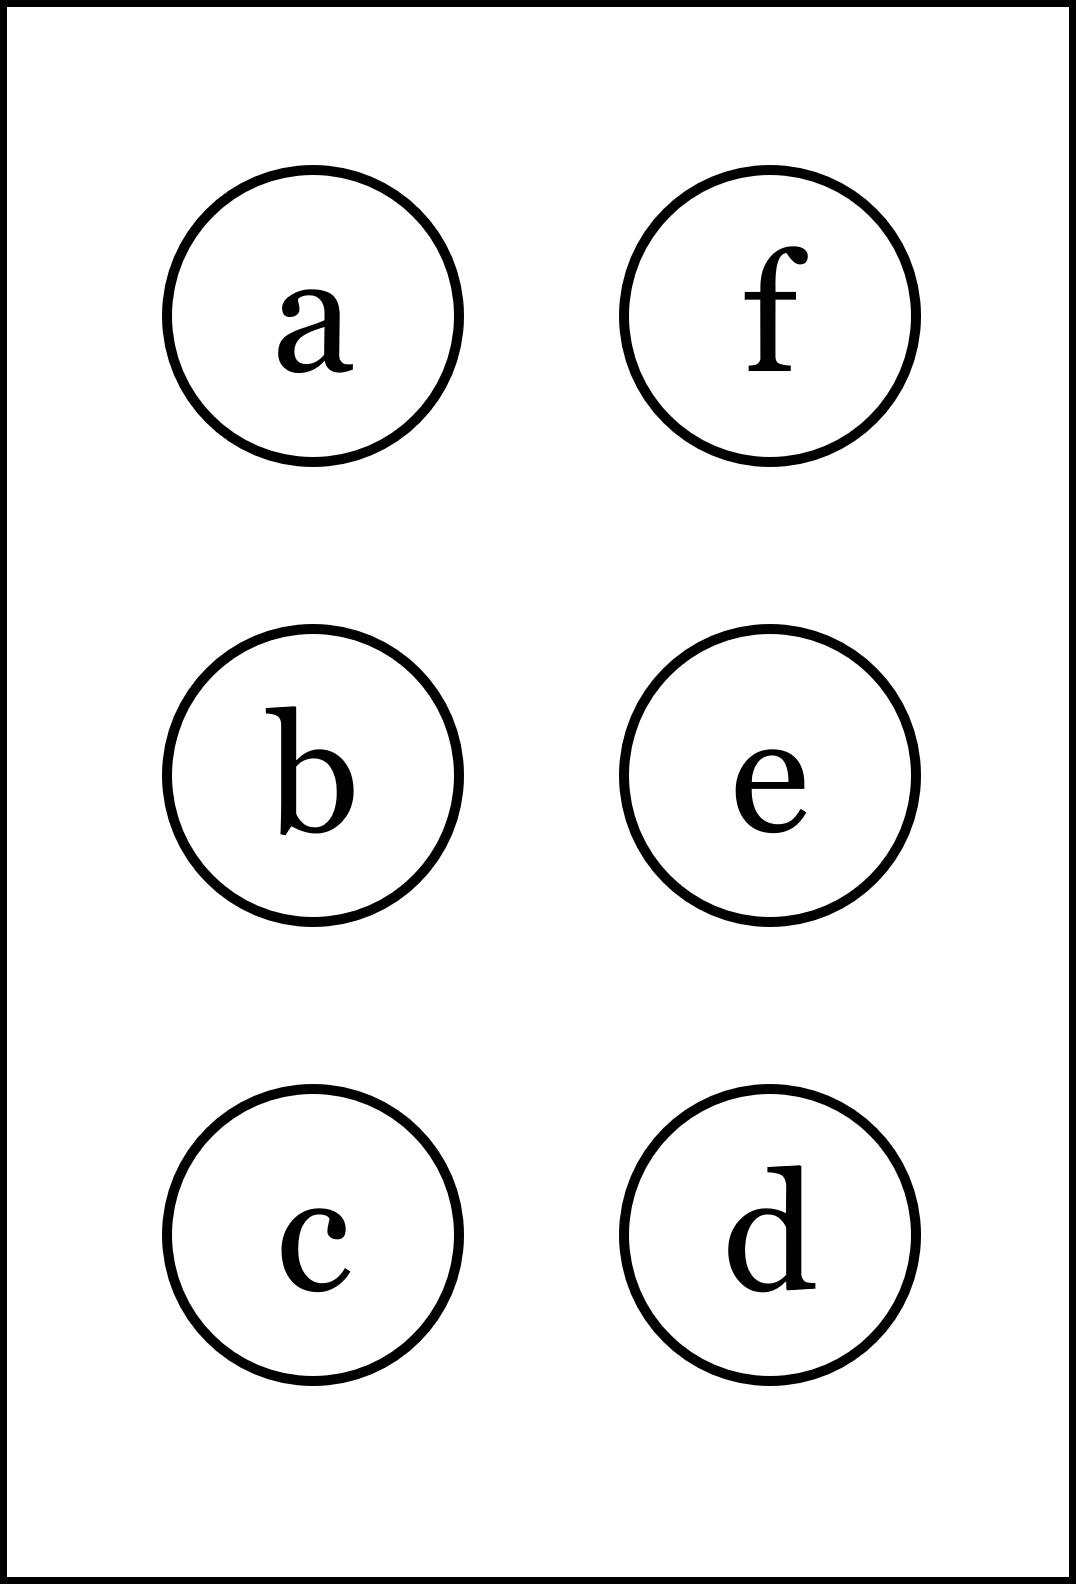
\includegraphics[height=40mm]{../images/braille.png}
{\small Písmeno Braillovej abecedy}
\end{center}
\end{minipage}
\end{center}
\end{minipage}
%
\end{tabular}
\begin{tikzpicture}[remember picture,overlay]\node[xshift=7mm,yshift=-100.6mm,anchor=north west] at (current page.north west){\ding{33}};\end{tikzpicture}
\begin{tikzpicture}[remember picture,overlay]\node[xshift=151.2mm,yshift=-7mm,anchor=north west,rotate=270] at (current page.north west){\ding{33}};\end{tikzpicture}
\newpage
\thispagestyle{empty}
\begin{tabular}{c:c}
\begin{minipage}[c][99mm][t]{0.49\linewidth}
\begin{center}
\vspace{7mm}
{\huge Definiční obor, skupina \textit{Eta $\eta$} -\romannumeral1}\\[4.5mm]
\textit{Meno:}\phantom{xxxxxxxxxxxxxxxxxxxxxxxxxxxxxxxxxxxxxxxxxxxxxxxxxxxxxxxxxxxxxxxxx}\\[3.5mm]
\textbf{Zjisti definiční obor} zadaných funkcí. Pokud se shoduje s tím za otazníky,\\tak napravo obarvi příslušející kroužek načerno. \textbf{Spolu odevzdejte výsledné slovo}.\\[3mm]
\begin{minipage}{0.77\linewidth}
\begin{center}
\begin{varwidth}{\textwidth}
\begin{enumerate}
\normalsize
\item $f(x)=\cfrac{-2x-1}{4x+4}$\quad \dotfill\; ???\;\dotfill \quad $\mathbb{R}\smallsetminus\{-1\}$
\item $f(x)=\cfrac{1}{-3x^3+12x^2+45x-54}$\quad \dotfill\; ???\;\dotfill \quad $\mathbb{R}\smallsetminus\{1,-3,6\}$
\item $f(x)=4\sqrt{6x+5}$\quad \dotfill\; ???\;\dotfill \quad $x\leq\nicefrac{-5}{6}$
\item $f(x)=\sqrt{-x^2+5x}$\quad \dotfill\; ???\;\dotfill \quad $x\in\langle-5 , 0\rangle$
\item $f(x)=6\ln{(5x-2)}$\quad \dotfill\; ???\;\dotfill \quad $x>\nicefrac{2}{5}$
\item $f(x)=\ln{(x^2+7x+6)}$\quad \dotfill\; ???\;\dotfill \quad $x\in(-6 , -1)$
\end{enumerate}
\end{varwidth}
\end{center}
\end{minipage}
\begin{minipage}{0.20\linewidth}
\begin{center}
{\Huge\bfseries 1.} \\[2mm]
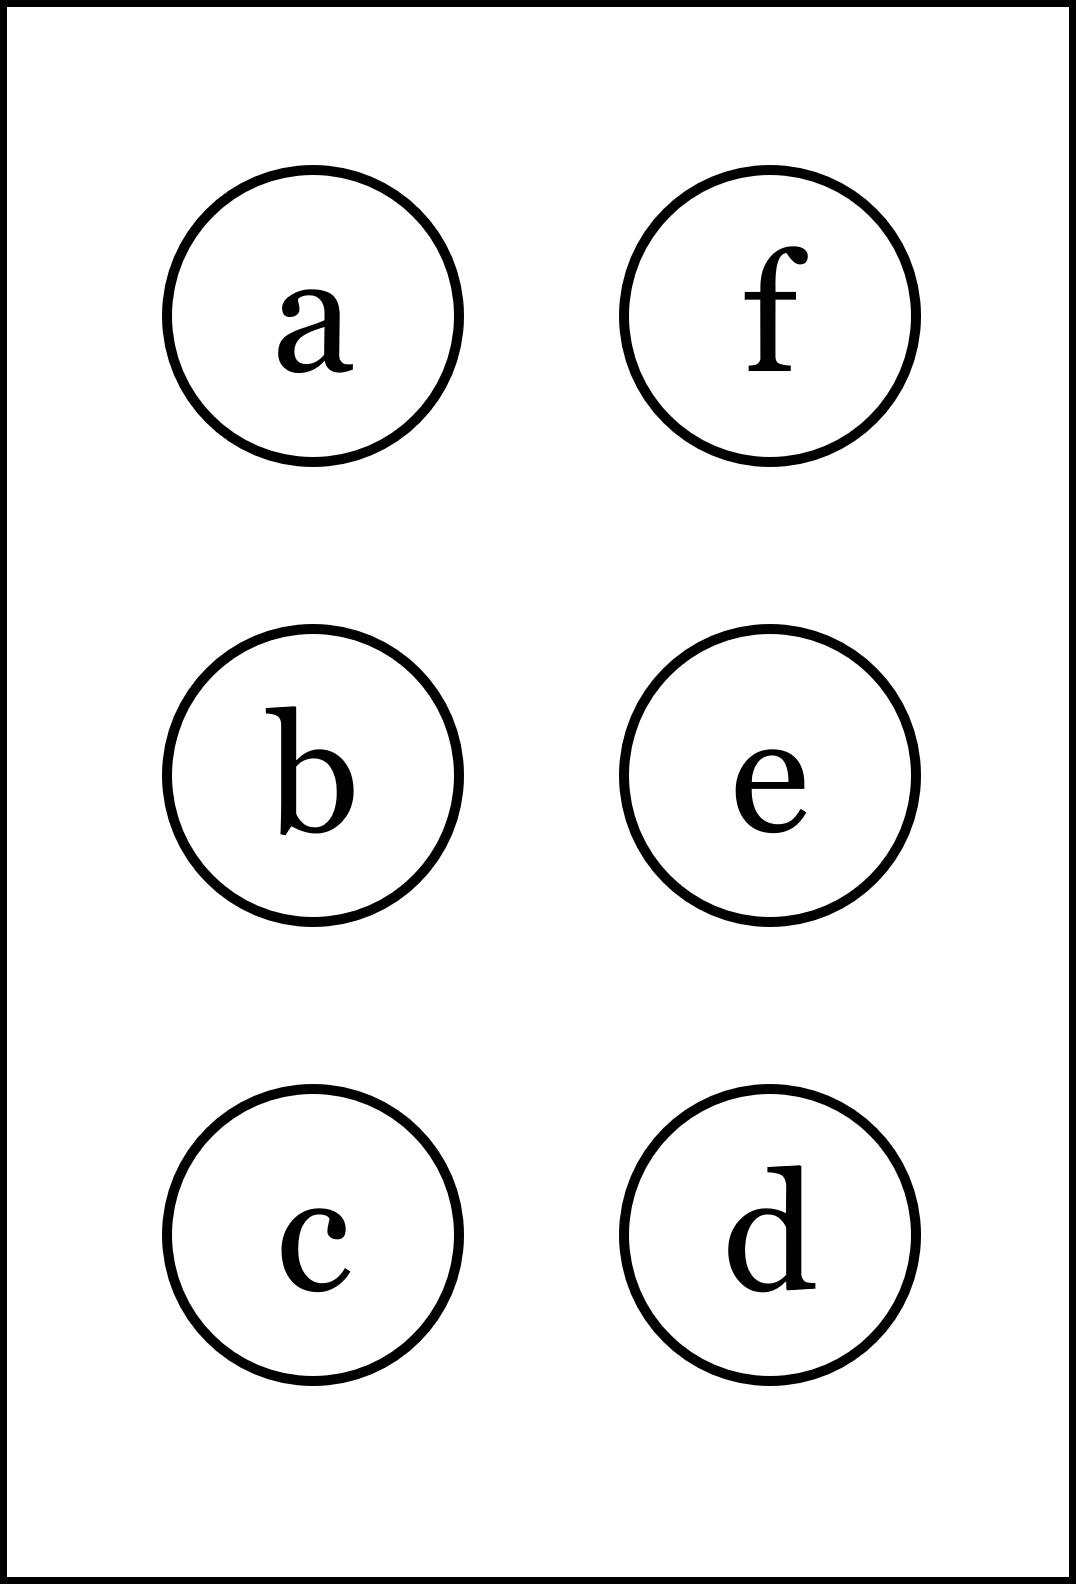
\includegraphics[height=40mm]{../images/braille.png}
{\small Písmeno Braillovej abecedy}
\end{center}
\end{minipage}
\end{center}
\end{minipage}
&
\begin{minipage}[c][99mm][t]{0.49\linewidth}
\begin{center}
\vspace{7mm}
{\huge Definiční obor, skupina \textit{Eta $\eta$} -\romannumeral2}\\[4.5mm]
\textit{Meno:}\phantom{xxxxxxxxxxxxxxxxxxxxxxxxxxxxxxxxxxxxxxxxxxxxxxxxxxxxxxxxxxxxxxxxx}\\[3.5mm]
\textbf{Zjisti definiční obor} zadaných funkcí. Pokud se shoduje s tím za otazníky,\\tak napravo obarvi příslušející kroužek načerno. \textbf{Spolu odevzdejte výsledné slovo}.\\[3mm]
\begin{minipage}{0.77\linewidth}
\begin{center}
\begin{varwidth}{\textwidth}
\begin{enumerate}
\normalsize
\item $f(x)=\cfrac{3x+5}{2x+2}$\quad \dotfill\; ???\;\dotfill \quad $\mathbb{R}\smallsetminus\{-1\}$
\item $f(x)=\cfrac{1}{3x^3-12x^2-3x+12}$\quad \dotfill\; ???\;\dotfill \quad $\mathbb{R}\smallsetminus\{1,4,-1\}$
\item $f(x)=-4\sqrt{-6x+7}$\quad \dotfill\; ???\;\dotfill \quad $x\leq\nicefrac{7}{6}$
\item $f(x)=\sqrt{-x^2-8x}$\quad \dotfill\; ???\;\dotfill \quad $x\in(-8 , 0)$
\item $f(x)=5\ln{(-5x-1)}$\quad \dotfill\; ???\;\dotfill \quad $x<\nicefrac{-1}{5}$
\item $f(x)=\ln{(x^2+x-42)}$\quad \dotfill\; ???\;\dotfill \quad $x\in(-7 , 6)$
\end{enumerate}
\end{varwidth}
\end{center}
\end{minipage}
\begin{minipage}{0.20\linewidth}
\begin{center}
{\Huge\bfseries 2.} \\[2mm]
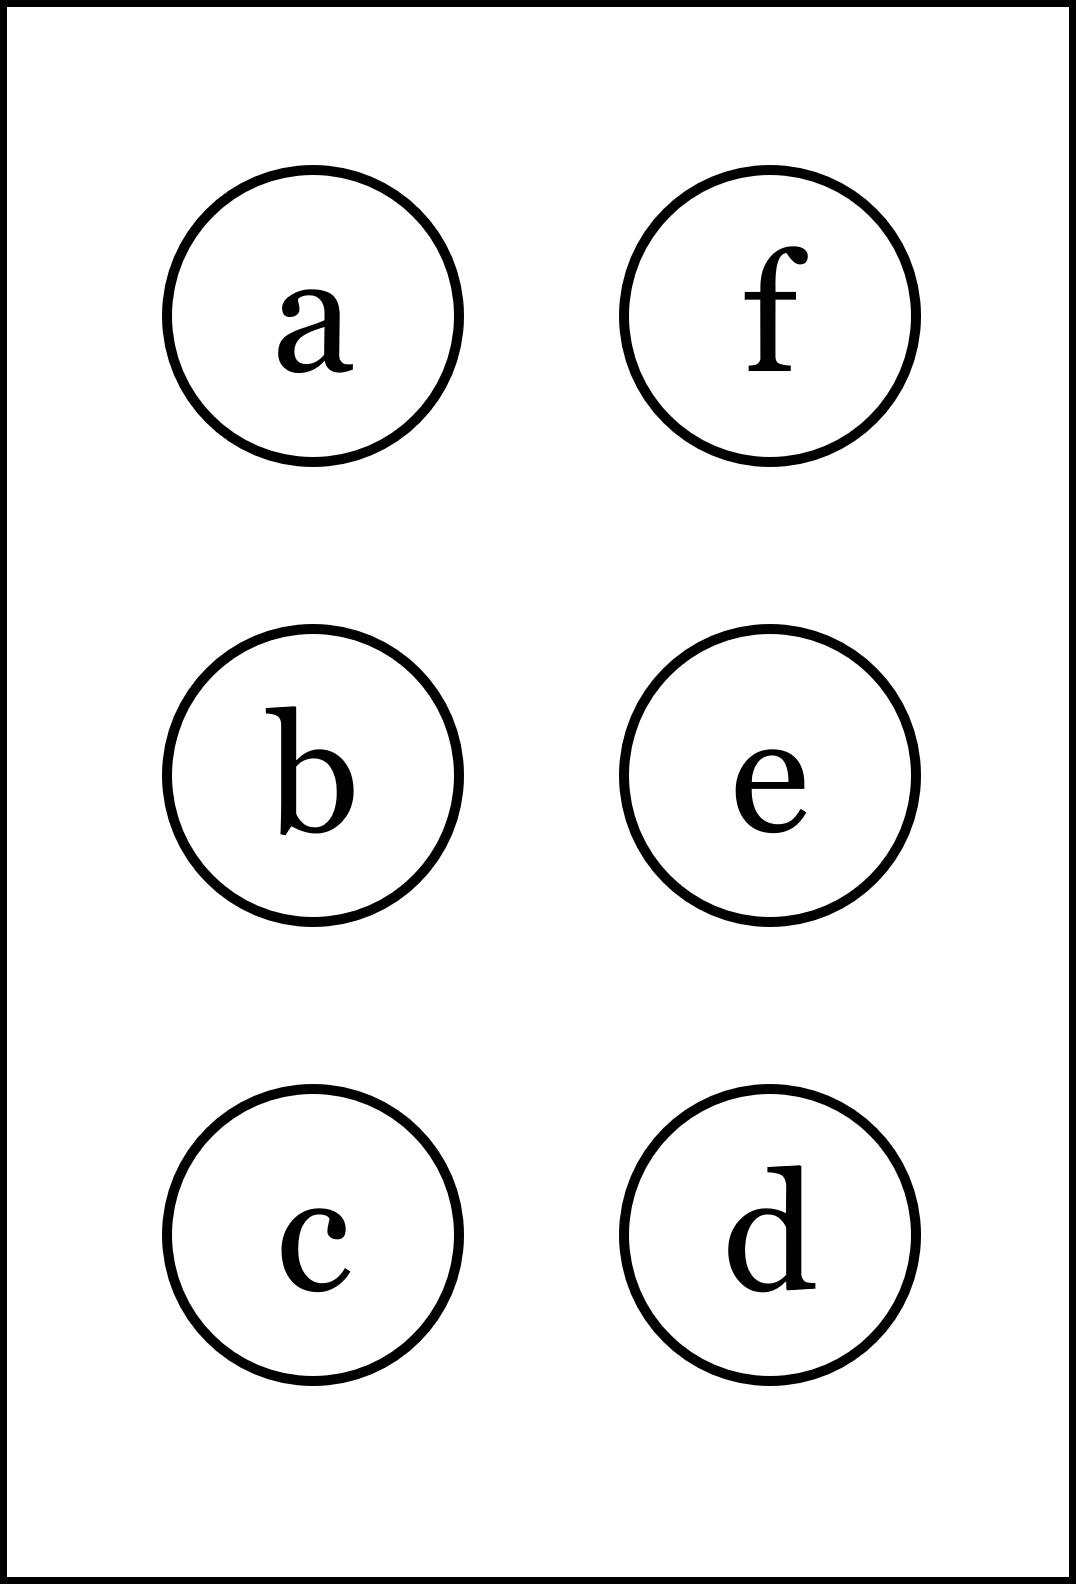
\includegraphics[height=40mm]{../images/braille.png}
{\small Písmeno Braillovej abecedy}
\end{center}
\end{minipage}
\end{center}
\end{minipage}
\\ \hdashline
\begin{minipage}[c][99mm][t]{0.49\linewidth}
\begin{center}
\vspace{7mm}
{\huge Definiční obor, skupina \textit{Eta $\eta$} -\romannumeral3}\\[4.5mm]
\textit{Meno:}\phantom{xxxxxxxxxxxxxxxxxxxxxxxxxxxxxxxxxxxxxxxxxxxxxxxxxxxxxxxxxxxxxxxxx}\\[3.5mm]
\textbf{Zjisti definiční obor} zadaných funkcí. Pokud se shoduje s tím za otazníky,\\tak napravo obarvi příslušející kroužek načerno. \textbf{Spolu odevzdejte výsledné slovo}.\\[3mm]
\begin{minipage}{0.77\linewidth}
\begin{center}
\begin{varwidth}{\textwidth}
\begin{enumerate}
\normalsize
\item $f(x)=\cfrac{-2x+3}{x+5}$\quad \dotfill\; ???\;\dotfill \quad $\mathbb{R}\smallsetminus\{-5\}$
\item $f(x)=\cfrac{1}{-x^3-9x^2-23x-15}$\quad \dotfill\; ???\;\dotfill \quad $\mathbb{R}\smallsetminus\{-5,-3,-1\}$
\item $f(x)=8\sqrt{3x-3}$\quad \dotfill\; ???\;\dotfill \quad $x\geq1$
\item $f(x)=\sqrt{-x^2-3x}$\quad \dotfill\; ???\;\dotfill \quad $x\in\langle0 , 3\rangle$
\item $f(x)=2\ln{(-3x+5)}$\quad \dotfill\; ???\;\dotfill \quad $x<\nicefrac{5}{3}$
\item $f(x)=\ln{(x^2+4x+3)}$\quad \dotfill\; ???\;\dotfill \quad $x\in(-3 , -1)$
\end{enumerate}
\end{varwidth}
\end{center}
\end{minipage}
\begin{minipage}{0.20\linewidth}
\begin{center}
{\Huge\bfseries 3.} \\[2mm]
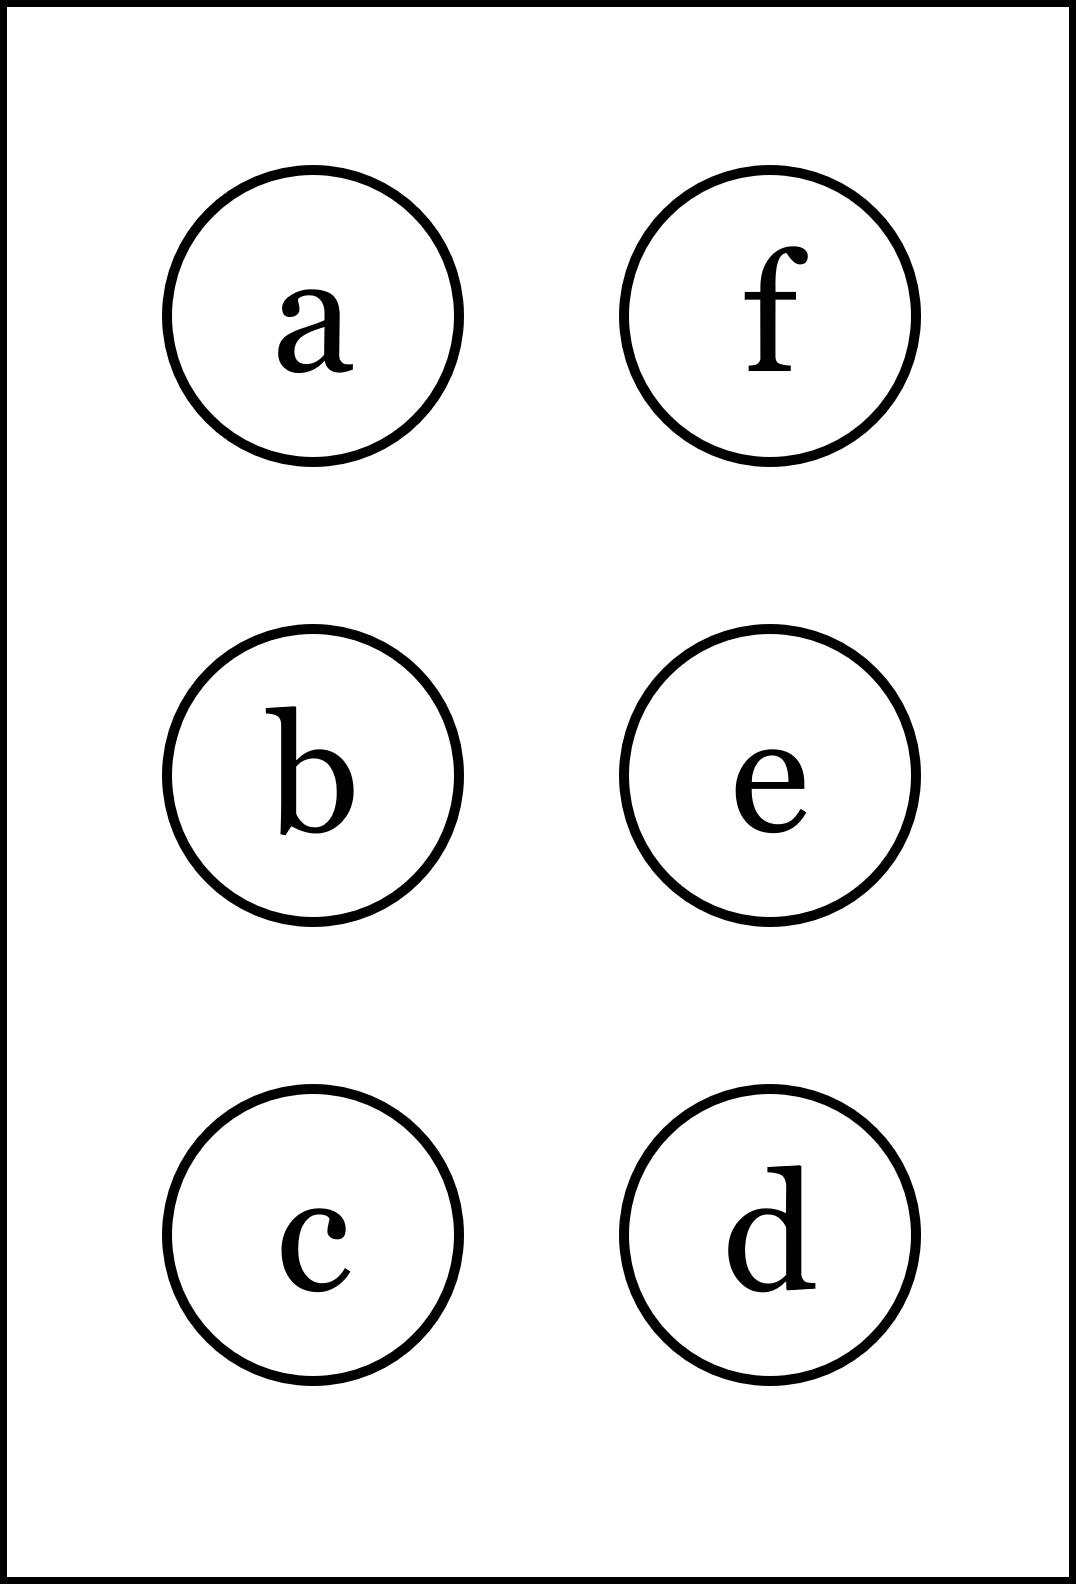
\includegraphics[height=40mm]{../images/braille.png}
{\small Písmeno Braillovej abecedy}
\end{center}
\end{minipage}
\end{center}
\end{minipage}
&
\begin{minipage}[c][99mm][t]{0.49\linewidth}
\begin{center}
\vspace{7mm}
{\huge Definiční obor, skupina \textit{Eta $\eta$} -\romannumeral4}\\[4.5mm]
\textit{Meno:}\phantom{xxxxxxxxxxxxxxxxxxxxxxxxxxxxxxxxxxxxxxxxxxxxxxxxxxxxxxxxxxxxxxxxx}\\[3.5mm]
\textbf{Zjisti definiční obor} zadaných funkcí. Pokud se shoduje s tím za otazníky,\\tak napravo obarvi příslušející kroužek načerno. \textbf{Spolu odevzdejte výsledné slovo}.\\[3mm]
\begin{minipage}{0.77\linewidth}
\begin{center}
\begin{varwidth}{\textwidth}
\begin{enumerate}
\normalsize
\item $f(x)=\cfrac{x-2}{x-1}$\quad \dotfill\; ???\;\dotfill \quad $\mathbb{R}\smallsetminus\{1\}$
\item $f(x)=\cfrac{1}{4x^3+16x^2+20x+8}$\quad \dotfill\; ???\;\dotfill \quad $\mathbb{R}\smallsetminus\{0,2,-1\}$
\item $f(x)=-3\sqrt{-2x+5}$\quad \dotfill\; ???\;\dotfill \quad $x\geq\nicefrac{5}{2}$
\item $f(x)=\sqrt{-x^2+x}$\quad \dotfill\; ???\;\dotfill \quad $x\in(0 , 1)$
\item $f(x)=-2\ln{(x-3)}$\quad \dotfill\; ???\;\dotfill \quad $x>-3$
\item $f(x)=\ln{(x^2+x-6)}$\quad \dotfill\; ???\;\dotfill \quad $x\in(-3 , 2)$
\end{enumerate}
\end{varwidth}
\end{center}
\end{minipage}
\begin{minipage}{0.20\linewidth}
\begin{center}
{\Huge\bfseries 4.} \\[2mm]
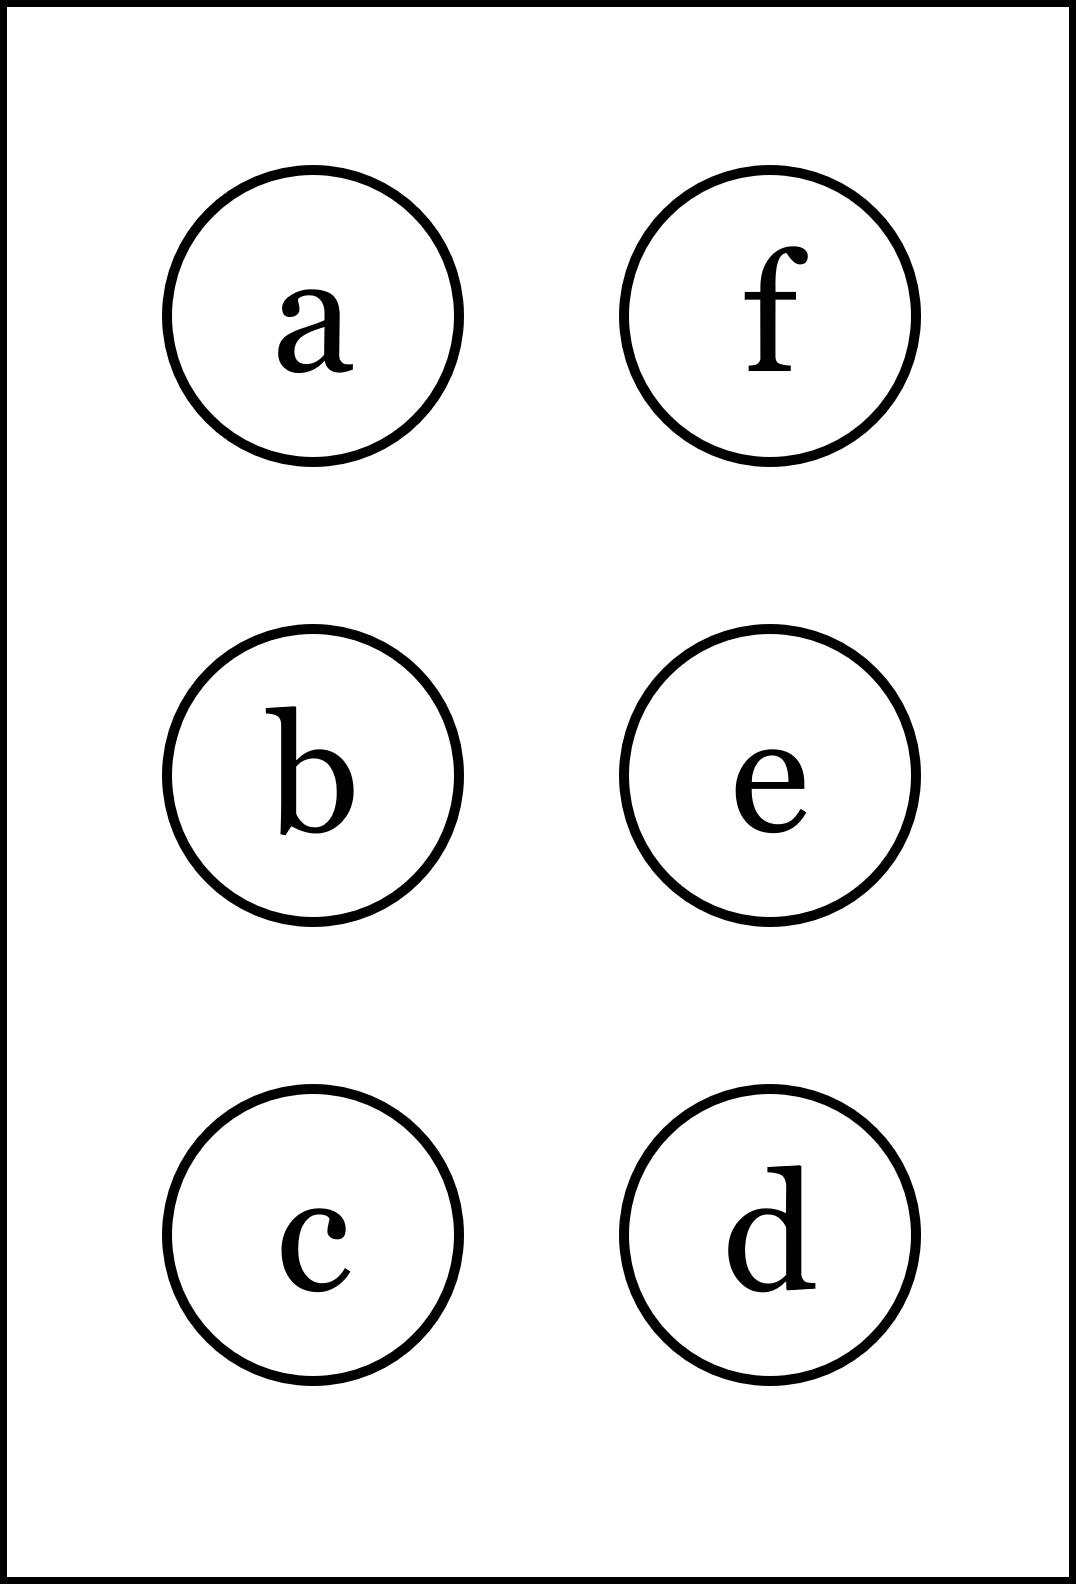
\includegraphics[height=40mm]{../images/braille.png}
{\small Písmeno Braillovej abecedy}
\end{center}
\end{minipage}
\end{center}
\end{minipage}
%
\end{tabular}
\begin{tikzpicture}[remember picture,overlay]\node[xshift=7mm,yshift=-100.6mm,anchor=north west] at (current page.north west){\ding{33}};\end{tikzpicture}
\begin{tikzpicture}[remember picture,overlay]\node[xshift=151.2mm,yshift=-7mm,anchor=north west,rotate=270] at (current page.north west){\ding{33}};\end{tikzpicture}
\newpage
\thispagestyle{empty}
\begin{tabular}{c:c}
\begin{minipage}[c][99mm][t]{0.49\linewidth}
\begin{center}
\vspace{7mm}
{\huge Definiční obor, skupina \textit{Theta $\theta$} -\romannumeral1}\\[4.5mm]
\textit{Meno:}\phantom{xxxxxxxxxxxxxxxxxxxxxxxxxxxxxxxxxxxxxxxxxxxxxxxxxxxxxxxxxxxxxxxxx}\\[3.5mm]
\textbf{Zjisti definiční obor} zadaných funkcí. Pokud se shoduje s tím za otazníky,\\tak napravo obarvi příslušející kroužek načerno. \textbf{Spolu odevzdejte výsledné slovo}.\\[3mm]
\begin{minipage}{0.77\linewidth}
\begin{center}
\begin{varwidth}{\textwidth}
\begin{enumerate}
\normalsize
\item $f(x)=\cfrac{3x-5}{-8x-6}$\quad \dotfill\; ???\;\dotfill \quad $\mathbb{R}\smallsetminus\{\nicefrac{3}{4}\}$
\item $f(x)=\cfrac{1}{2x^3-12x^2+22x-12}$\quad \dotfill\; ???\;\dotfill \quad $\mathbb{R}\smallsetminus\{1,2,3\}$
\item $f(x)=-7\sqrt{9x-3}$\quad \dotfill\; ???\;\dotfill \quad $x\leq\nicefrac{1}{3}$
\item $f(x)=\sqrt{-x^2+2x}$\quad \dotfill\; ???\;\dotfill \quad $x\in\langle-2 , 0\rangle$
\item $f(x)=5\ln{(2x+5)}$\quad \dotfill\; ???\;\dotfill \quad $x>\nicefrac{-5}{2}$
\item $f(x)=\ln{(x^2-11x+18)}$\quad \dotfill\; ???\;\dotfill \quad $x\in(-\infty , 2)\cup(9 , \infty)$
\end{enumerate}
\end{varwidth}
\end{center}
\end{minipage}
\begin{minipage}{0.20\linewidth}
\begin{center}
{\Huge\bfseries 1.} \\[2mm]
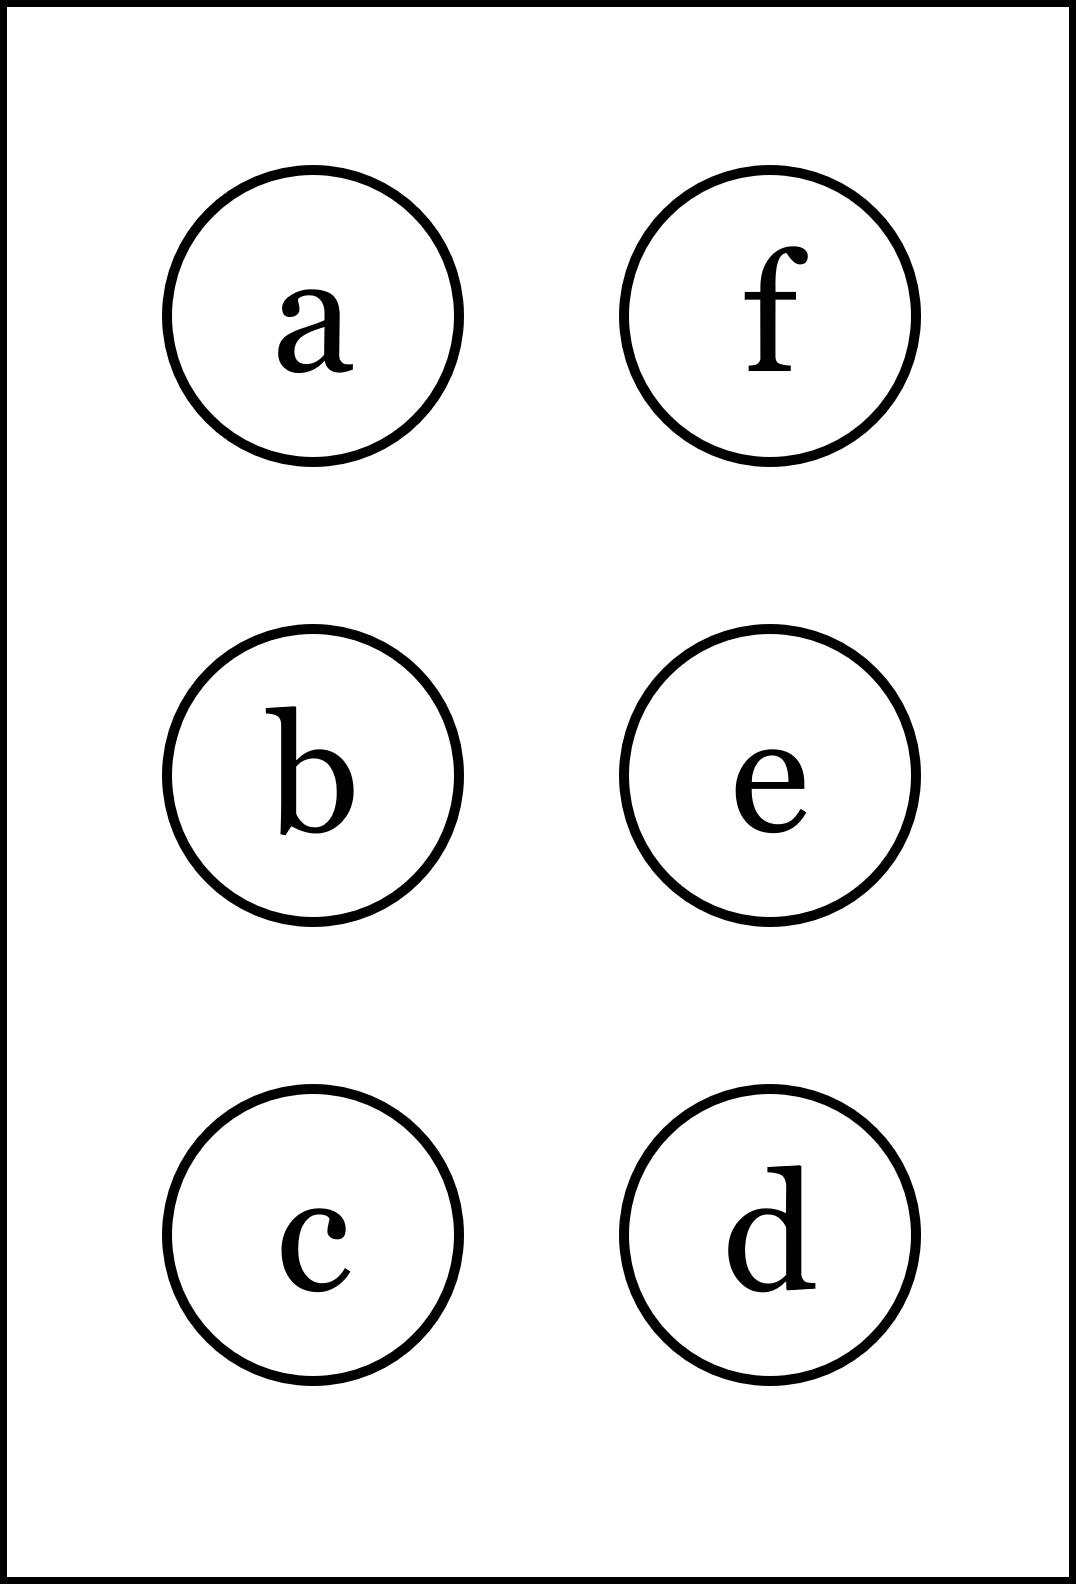
\includegraphics[height=40mm]{../images/braille.png}
{\small Písmeno Braillovej abecedy}
\end{center}
\end{minipage}
\end{center}
\end{minipage}
&
\begin{minipage}[c][99mm][t]{0.49\linewidth}
\begin{center}
\vspace{7mm}
{\huge Definiční obor, skupina \textit{Theta $\theta$} -\romannumeral2}\\[4.5mm]
\textit{Meno:}\phantom{xxxxxxxxxxxxxxxxxxxxxxxxxxxxxxxxxxxxxxxxxxxxxxxxxxxxxxxxxxxxxxxxx}\\[3.5mm]
\textbf{Zjisti definiční obor} zadaných funkcí. Pokud se shoduje s tím za otazníky,\\tak napravo obarvi příslušející kroužek načerno. \textbf{Spolu odevzdejte výsledné slovo}.\\[3mm]
\begin{minipage}{0.77\linewidth}
\begin{center}
\begin{varwidth}{\textwidth}
\begin{enumerate}
\normalsize
\item $f(x)=\cfrac{-9x-3}{x+1}$\quad \dotfill\; ???\;\dotfill \quad $\mathbb{R}\smallsetminus\{-1\}$
\item $f(x)=\cfrac{1}{6x^3-12x^2-24x+48}$\quad \dotfill\; ???\;\dotfill \quad $\mathbb{R}\smallsetminus\{4,-2\}$
\item $f(x)=2\sqrt{-9x+8}$\quad \dotfill\; ???\;\dotfill \quad $x\leq\nicefrac{8}{9}$
\item $f(x)=\sqrt{-x^2+8x}$\quad \dotfill\; ???\;\dotfill \quad $x\in(0 , 8)$
\item $f(x)=7\ln{(-x-2)}$\quad \dotfill\; ???\;\dotfill \quad $x<-2$
\item $f(x)=\ln{(x^2+3x-4)}$\quad \dotfill\; ???\;\dotfill \quad $x\in(-4 , 1)$
\end{enumerate}
\end{varwidth}
\end{center}
\end{minipage}
\begin{minipage}{0.20\linewidth}
\begin{center}
{\Huge\bfseries 2.} \\[2mm]
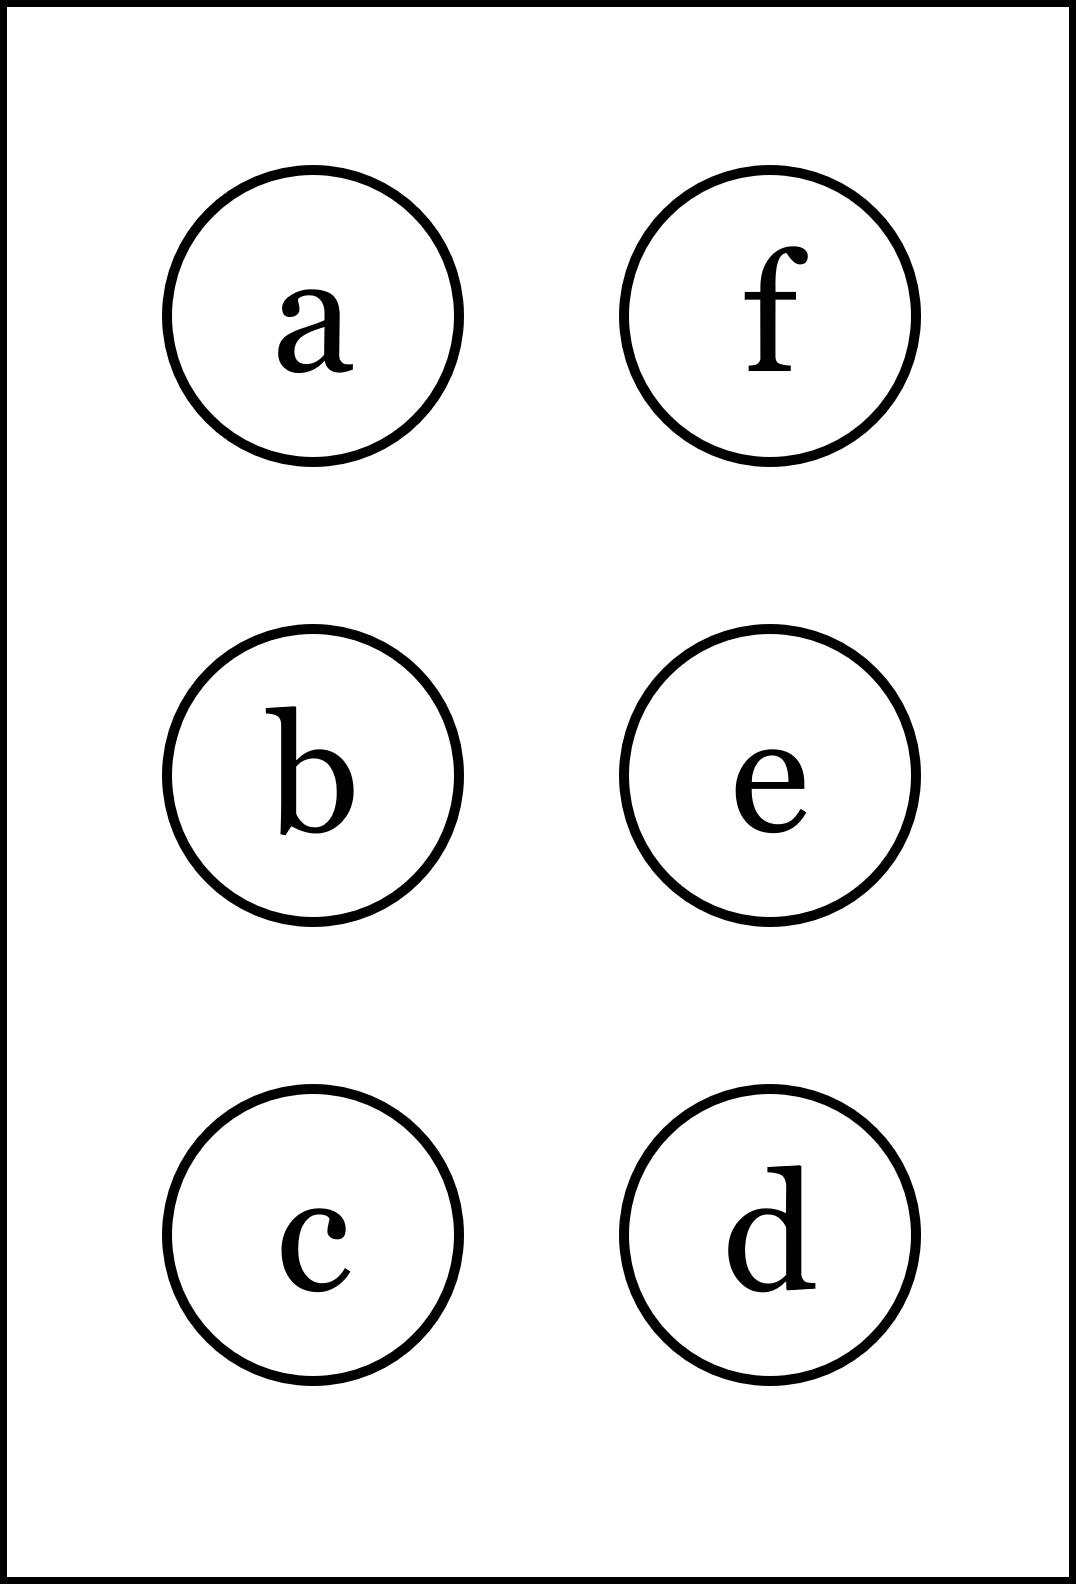
\includegraphics[height=40mm]{../images/braille.png}
{\small Písmeno Braillovej abecedy}
\end{center}
\end{minipage}
\end{center}
\end{minipage}
\\ \hdashline
\begin{minipage}[c][99mm][t]{0.49\linewidth}
\begin{center}
\vspace{7mm}
{\huge Definiční obor, skupina \textit{Theta $\theta$} -\romannumeral3}\\[4.5mm]
\textit{Meno:}\phantom{xxxxxxxxxxxxxxxxxxxxxxxxxxxxxxxxxxxxxxxxxxxxxxxxxxxxxxxxxxxxxxxxx}\\[3.5mm]
\textbf{Zjisti definiční obor} zadaných funkcí. Pokud se shoduje s tím za otazníky,\\tak napravo obarvi příslušející kroužek načerno. \textbf{Spolu odevzdejte výsledné slovo}.\\[3mm]
\begin{minipage}{0.77\linewidth}
\begin{center}
\begin{varwidth}{\textwidth}
\begin{enumerate}
\normalsize
\item $f(x)=\cfrac{-8x+5}{x+6}$\quad \dotfill\; ???\;\dotfill \quad $\mathbb{R}\smallsetminus\{6\}$
\item $f(x)=\cfrac{1}{2x^3-14x^2+28x-16}$\quad \dotfill\; ???\;\dotfill \quad $\mathbb{R}\smallsetminus\{1,2,4\}$
\item $f(x)=-4\sqrt{2x+6}$\quad \dotfill\; ???\;\dotfill \quad $x\leq-3$
\item $f(x)=\sqrt{-x^2+2x}$\quad \dotfill\; ???\;\dotfill \quad $x\in(0 , 2)$
\item $f(x)=-5\ln{(-2x+3)}$\quad \dotfill\; ???\;\dotfill \quad $x<\nicefrac{3}{2}$
\item $f(x)=\ln{(x^2-2x+1)}$\quad \dotfill\; ???\;\dotfill \quad $x\in(-\infty , 1)\cup(1 , \infty)$
\end{enumerate}
\end{varwidth}
\end{center}
\end{minipage}
\begin{minipage}{0.20\linewidth}
\begin{center}
{\Huge\bfseries 3.} \\[2mm]
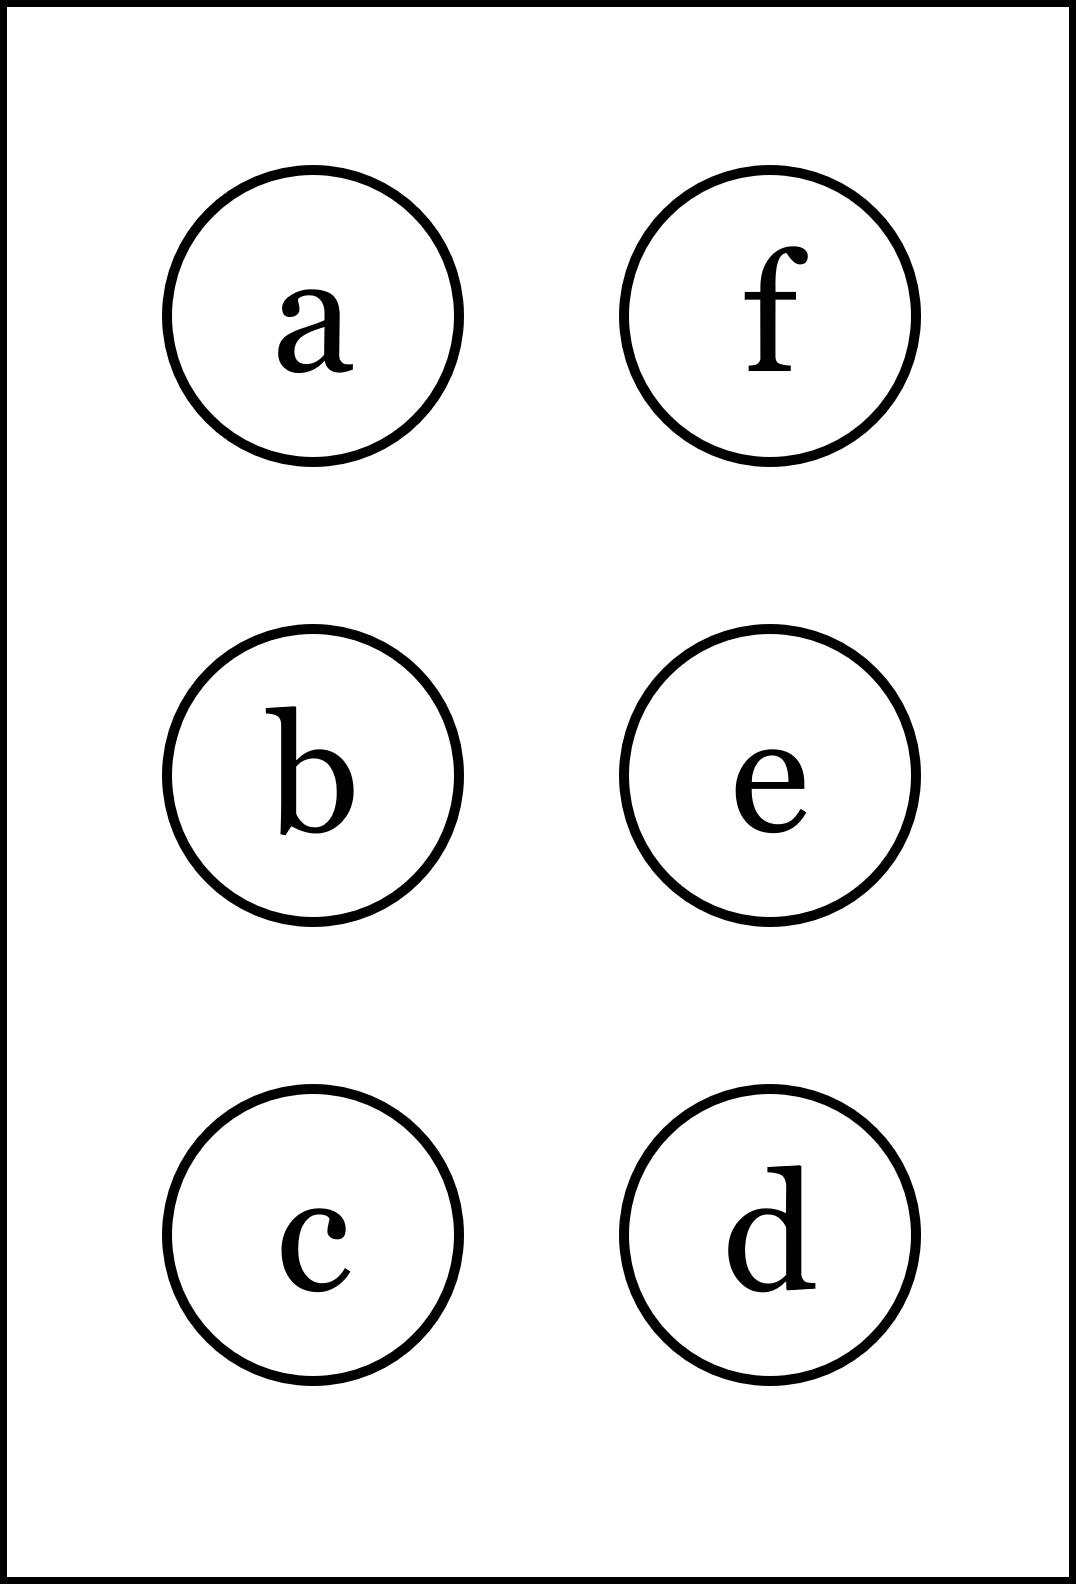
\includegraphics[height=40mm]{../images/braille.png}
{\small Písmeno Braillovej abecedy}
\end{center}
\end{minipage}
\end{center}
\end{minipage}
&
\begin{minipage}[c][99mm][t]{0.49\linewidth}
\begin{center}
\vspace{7mm}
{\huge Definiční obor, skupina \textit{Theta $\theta$} -\romannumeral4}\\[4.5mm]
\textit{Meno:}\phantom{xxxxxxxxxxxxxxxxxxxxxxxxxxxxxxxxxxxxxxxxxxxxxxxxxxxxxxxxxxxxxxxxx}\\[3.5mm]
\textbf{Zjisti definiční obor} zadaných funkcí. Pokud se shoduje s tím za otazníky,\\tak napravo obarvi příslušející kroužek načerno. \textbf{Spolu odevzdejte výsledné slovo}.\\[3mm]
\begin{minipage}{0.77\linewidth}
\begin{center}
\begin{varwidth}{\textwidth}
\begin{enumerate}
\normalsize
\item $f(x)=\cfrac{2x-9}{4x-5}$\quad \dotfill\; ???\;\dotfill \quad $\mathbb{R}\smallsetminus\{\nicefrac{5}{4}\}$
\item $f(x)=\cfrac{1}{-x^3-3x^2+34x-48}$\quad \dotfill\; ???\;\dotfill \quad $\mathbb{R}\smallsetminus\{-8,0,-3\}$
\item $f(x)=2\sqrt{3x-8}$\quad \dotfill\; ???\;\dotfill \quad $x\geq\nicefrac{8}{3}$
\item $f(x)=\sqrt{-x^2-7x}$\quad \dotfill\; ???\;\dotfill \quad $x\in(-7 , 0)$
\item $f(x)=-1\ln{(-4x+4)}$\quad \dotfill\; ???\;\dotfill \quad $x<1$
\item $f(x)=\ln{(x^2+6x-7)}$\quad \dotfill\; ???\;\dotfill \quad $x\in(-7 , 1)$
\end{enumerate}
\end{varwidth}
\end{center}
\end{minipage}
\begin{minipage}{0.20\linewidth}
\begin{center}
{\Huge\bfseries 4.} \\[2mm]
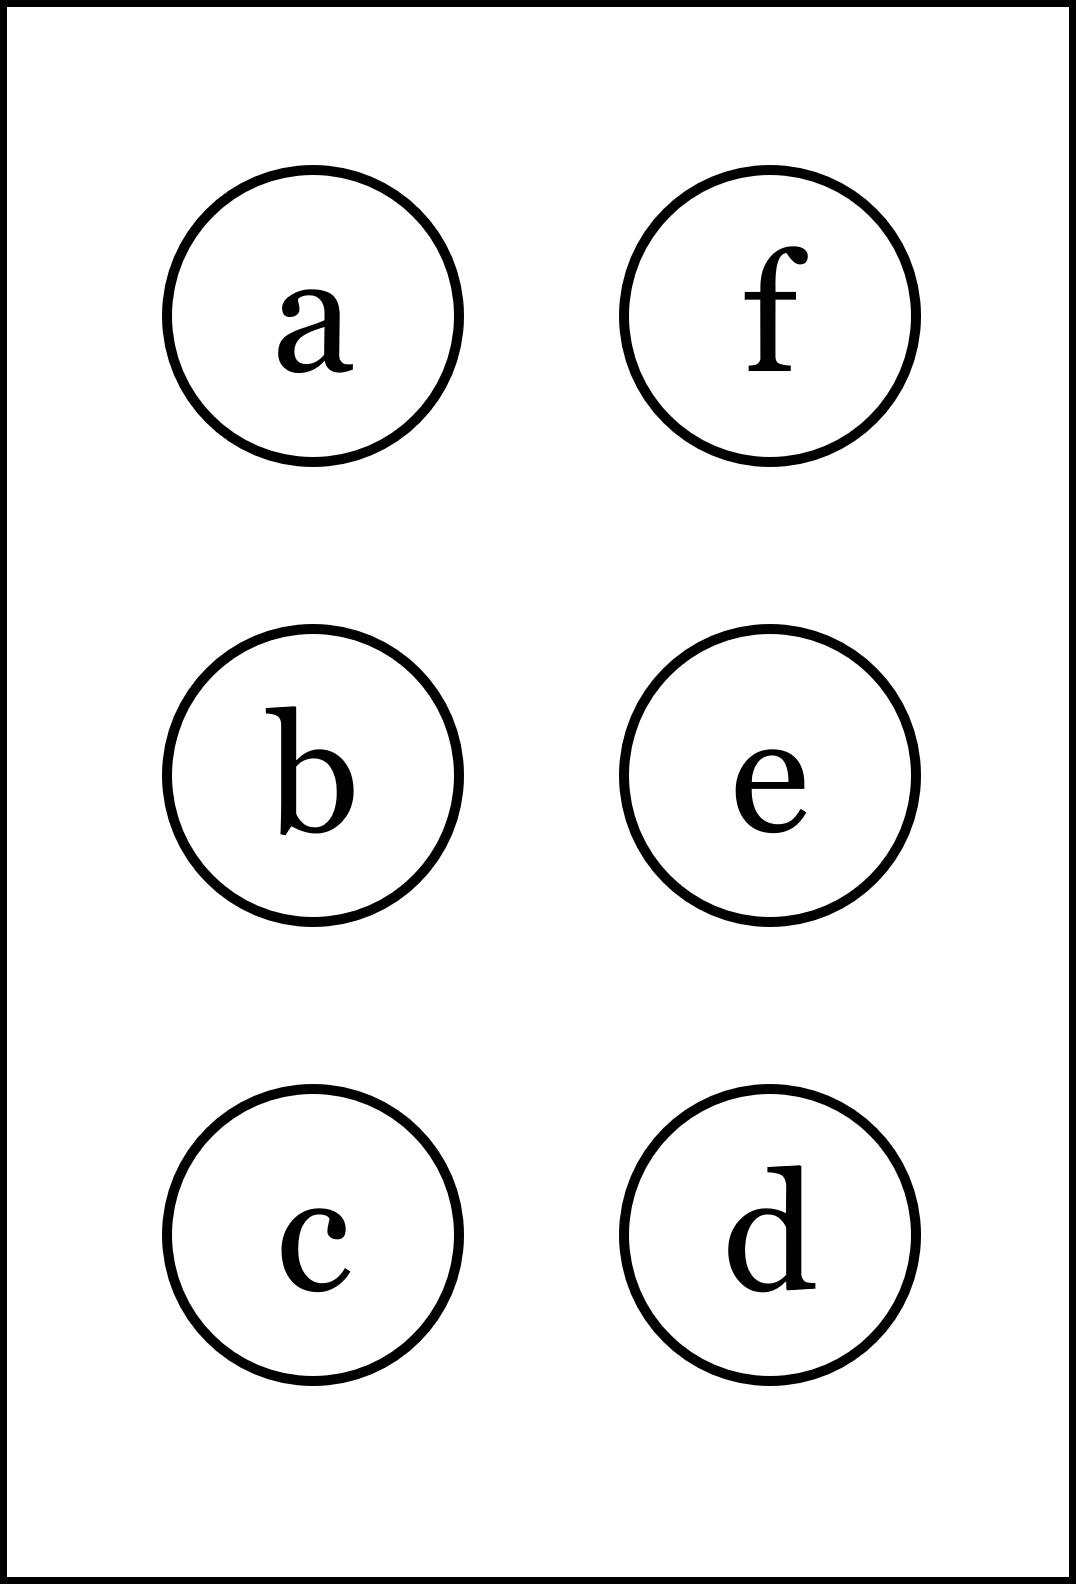
\includegraphics[height=40mm]{../images/braille.png}
{\small Písmeno Braillovej abecedy}
\end{center}
\end{minipage}
\end{center}
\end{minipage}
%
\end{tabular}
\begin{tikzpicture}[remember picture,overlay]\node[xshift=7mm,yshift=-100.6mm,anchor=north west] at (current page.north west){\ding{33}};\end{tikzpicture}
\begin{tikzpicture}[remember picture,overlay]\node[xshift=151.2mm,yshift=-7mm,anchor=north west,rotate=270] at (current page.north west){\ding{33}};\end{tikzpicture}
\newpage
\thispagestyle{empty}
\begin{tabular}{c:c}
\begin{minipage}[c][99mm][t]{0.49\linewidth}
\begin{center}
\vspace{7mm}
{\huge Definiční obor, skupina \textit{Iota $\iota$} -\romannumeral1}\\[4.5mm]
\textit{Meno:}\phantom{xxxxxxxxxxxxxxxxxxxxxxxxxxxxxxxxxxxxxxxxxxxxxxxxxxxxxxxxxxxxxxxxx}\\[3.5mm]
\textbf{Zjisti definiční obor} zadaných funkcí. Pokud se shoduje s tím za otazníky,\\tak napravo obarvi příslušející kroužek načerno. \textbf{Spolu odevzdejte výsledné slovo}.\\[3mm]
\begin{minipage}{0.77\linewidth}
\begin{center}
\begin{varwidth}{\textwidth}
\begin{enumerate}
\normalsize
\item $f(x)=\cfrac{-3x+3}{9x-2}$\quad \dotfill\; ???\;\dotfill \quad $\mathbb{R}\smallsetminus\{\nicefrac{2}{9}\}$
\item $f(x)=\cfrac{1}{x^3-7x^2-17x-9}$\quad \dotfill\; ???\;\dotfill \quad $\mathbb{R}\smallsetminus\{9,-1\}$
\item $f(x)=-3\sqrt{6x-3}$\quad \dotfill\; ???\;\dotfill \quad $x\geq\nicefrac{-1}{2}$
\item $f(x)=\sqrt{-x^2-x}$\quad \dotfill\; ???\;\dotfill \quad $x\in\langle0 , 1\rangle$
\item $f(x)=-7\ln{(7x-1)}$\quad \dotfill\; ???\;\dotfill \quad $x<\nicefrac{1}{7}$
\item $f(x)=\ln{(x^2-3x-10)}$\quad \dotfill\; ???\;\dotfill \quad $x\in(-2 , 5)$
\end{enumerate}
\end{varwidth}
\end{center}
\end{minipage}
\begin{minipage}{0.20\linewidth}
\begin{center}
{\Huge\bfseries 1.} \\[2mm]
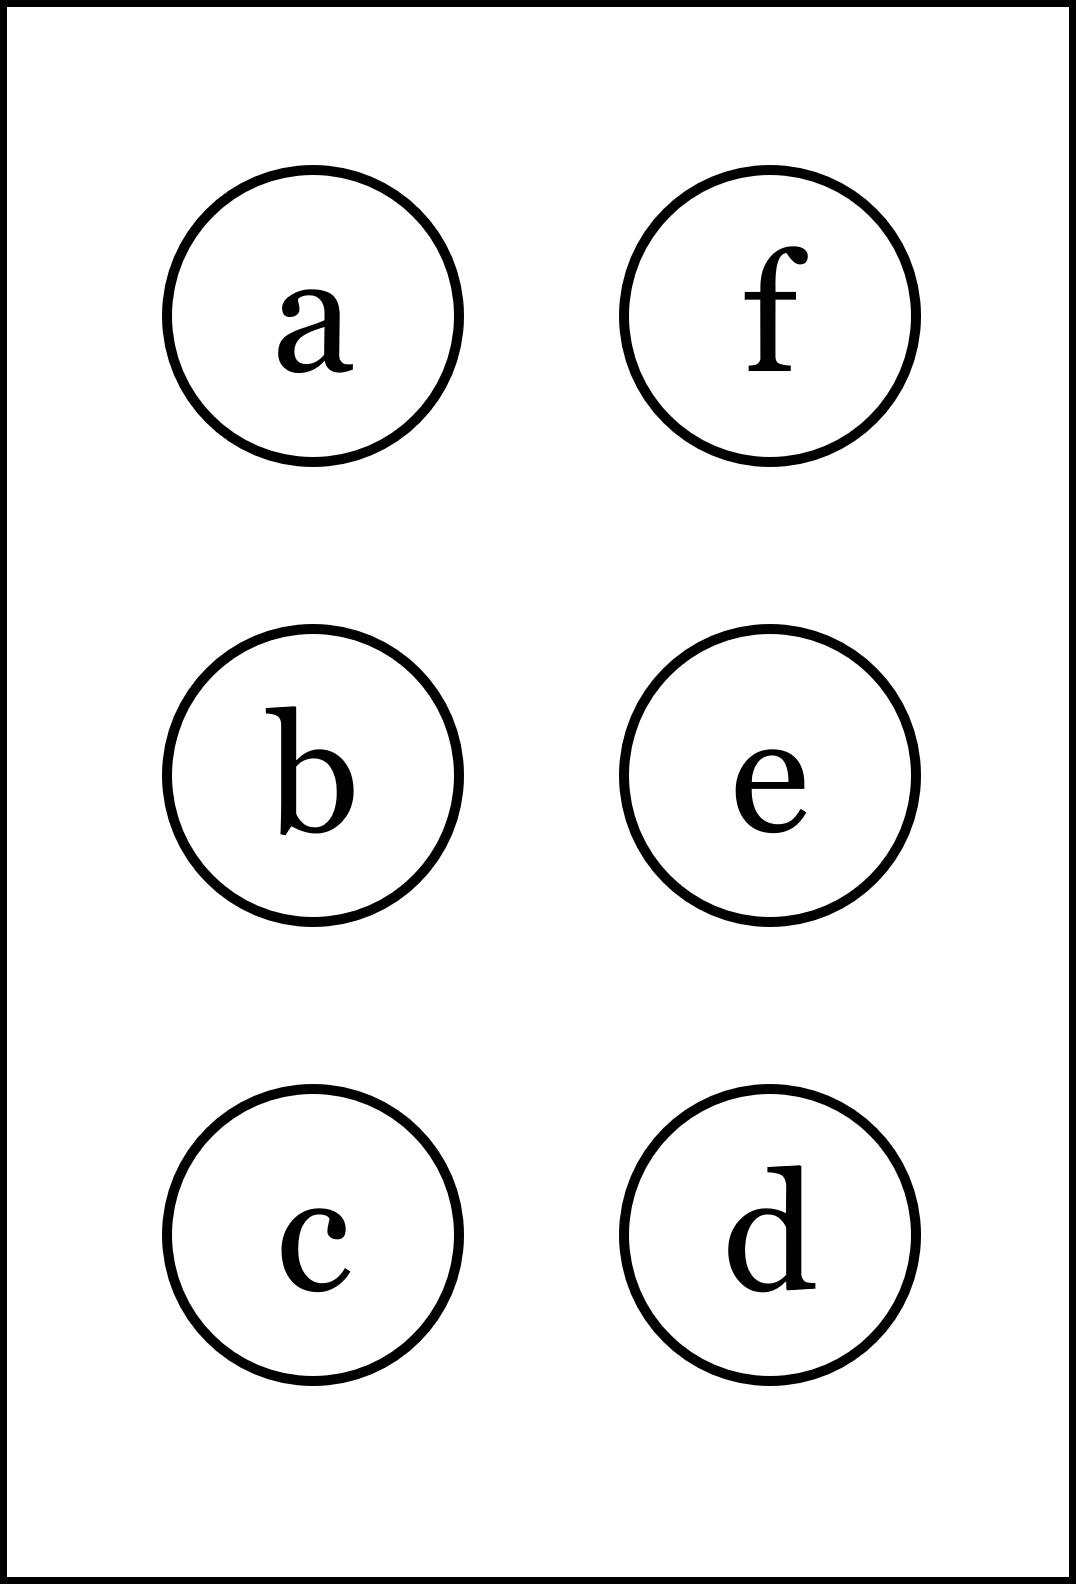
\includegraphics[height=40mm]{../images/braille.png}
{\small Písmeno Braillovej abecedy}
\end{center}
\end{minipage}
\end{center}
\end{minipage}
&
\begin{minipage}[c][99mm][t]{0.49\linewidth}
\begin{center}
\vspace{7mm}
{\huge Definiční obor, skupina \textit{Iota $\iota$} -\romannumeral2}\\[4.5mm]
\textit{Meno:}\phantom{xxxxxxxxxxxxxxxxxxxxxxxxxxxxxxxxxxxxxxxxxxxxxxxxxxxxxxxxxxxxxxxxx}\\[3.5mm]
\textbf{Zjisti definiční obor} zadaných funkcí. Pokud se shoduje s tím za otazníky,\\tak napravo obarvi příslušející kroužek načerno. \textbf{Spolu odevzdejte výsledné slovo}.\\[3mm]
\begin{minipage}{0.77\linewidth}
\begin{center}
\begin{varwidth}{\textwidth}
\begin{enumerate}
\normalsize
\item $f(x)=\cfrac{-5x+5}{-6x-1}$\quad \dotfill\; ???\;\dotfill \quad $\mathbb{R}\smallsetminus\{\nicefrac{-1}{6}\}$
\item $f(x)=\cfrac{1}{x^3-8x^2+4x+48}$\quad \dotfill\; ???\;\dotfill \quad $\mathbb{R}\smallsetminus\{2,4\}$
\item $f(x)=-2\sqrt{9x-2}$\quad \dotfill\; ???\;\dotfill \quad $x\leq\nicefrac{2}{9}$
\item $f(x)=\sqrt{-x^2+x}$\quad \dotfill\; ???\;\dotfill \quad $x\in\langle0 , 1\rangle$
\item $f(x)=-8\ln{(x-1)}$\quad \dotfill\; ???\;\dotfill \quad $x>-1$
\item $f(x)=\ln{(x^2+6x-7)}$\quad \dotfill\; ???\;\dotfill \quad $x\in(-7 , 1)$
\end{enumerate}
\end{varwidth}
\end{center}
\end{minipage}
\begin{minipage}{0.20\linewidth}
\begin{center}
{\Huge\bfseries 2.} \\[2mm]
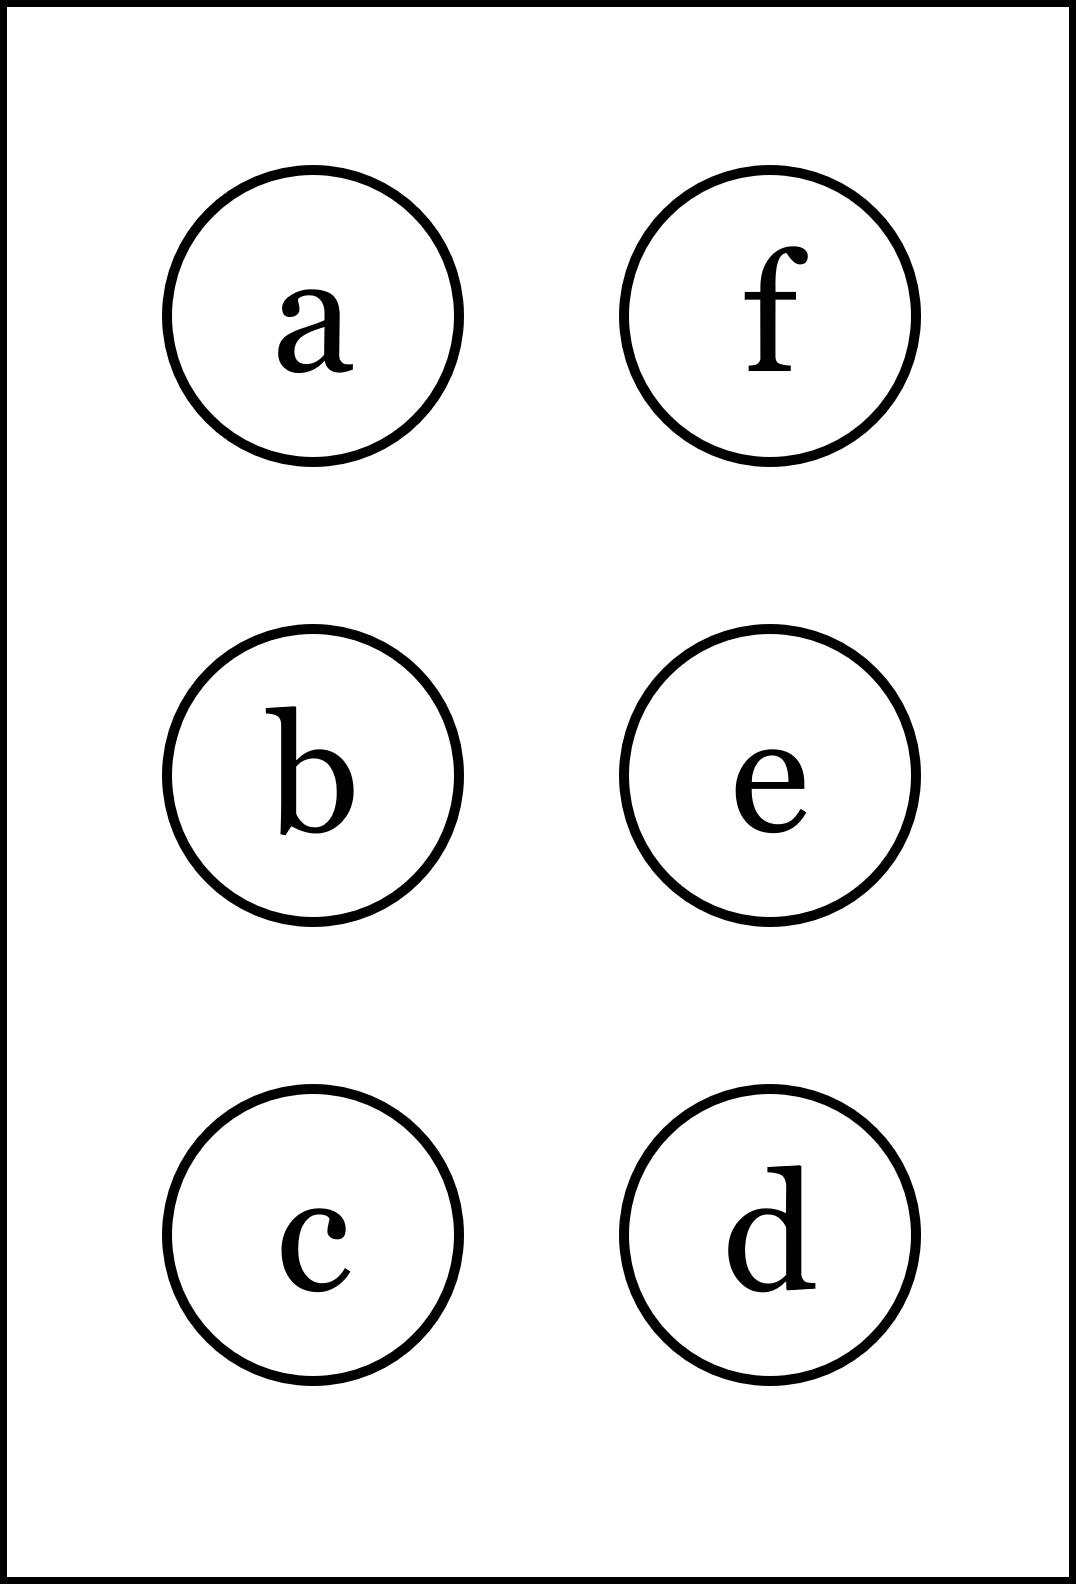
\includegraphics[height=40mm]{../images/braille.png}
{\small Písmeno Braillovej abecedy}
\end{center}
\end{minipage}
\end{center}
\end{minipage}
\\ \hdashline
\begin{minipage}[c][99mm][t]{0.49\linewidth}
\begin{center}
\vspace{7mm}
{\huge Definiční obor, skupina \textit{Iota $\iota$} -\romannumeral3}\\[4.5mm]
\textit{Meno:}\phantom{xxxxxxxxxxxxxxxxxxxxxxxxxxxxxxxxxxxxxxxxxxxxxxxxxxxxxxxxxxxxxxxxx}\\[3.5mm]
\textbf{Zjisti definiční obor} zadaných funkcí. Pokud se shoduje s tím za otazníky,\\tak napravo obarvi příslušející kroužek načerno. \textbf{Spolu odevzdejte výsledné slovo}.\\[3mm]
\begin{minipage}{0.77\linewidth}
\begin{center}
\begin{varwidth}{\textwidth}
\begin{enumerate}
\normalsize
\item $f(x)=\cfrac{-4x-5}{x+7}$\quad \dotfill\; ???\;\dotfill \quad $\mathbb{R}\smallsetminus\{-7\}$
\item $f(x)=\cfrac{1}{-x^3+6x^2-9x+4}$\quad \dotfill\; ???\;\dotfill \quad $\mathbb{R}\smallsetminus\{1,4\}$
\item $f(x)=1\sqrt{x-3}$\quad \dotfill\; ???\;\dotfill \quad $x\leq3$
\item $f(x)=\sqrt{-x^2+3x}$\quad \dotfill\; ???\;\dotfill \quad $x\in(0 , 3)$
\item $f(x)=2\ln{(-9x-7)}$\quad \dotfill\; ???\;\dotfill \quad $x<\nicefrac{7}{9}$
\item $f(x)=\ln{(x^2-4x+3)}$\quad \dotfill\; ???\;\dotfill \quad $x\in(1 , 3)$
\end{enumerate}
\end{varwidth}
\end{center}
\end{minipage}
\begin{minipage}{0.20\linewidth}
\begin{center}
{\Huge\bfseries 3.} \\[2mm]
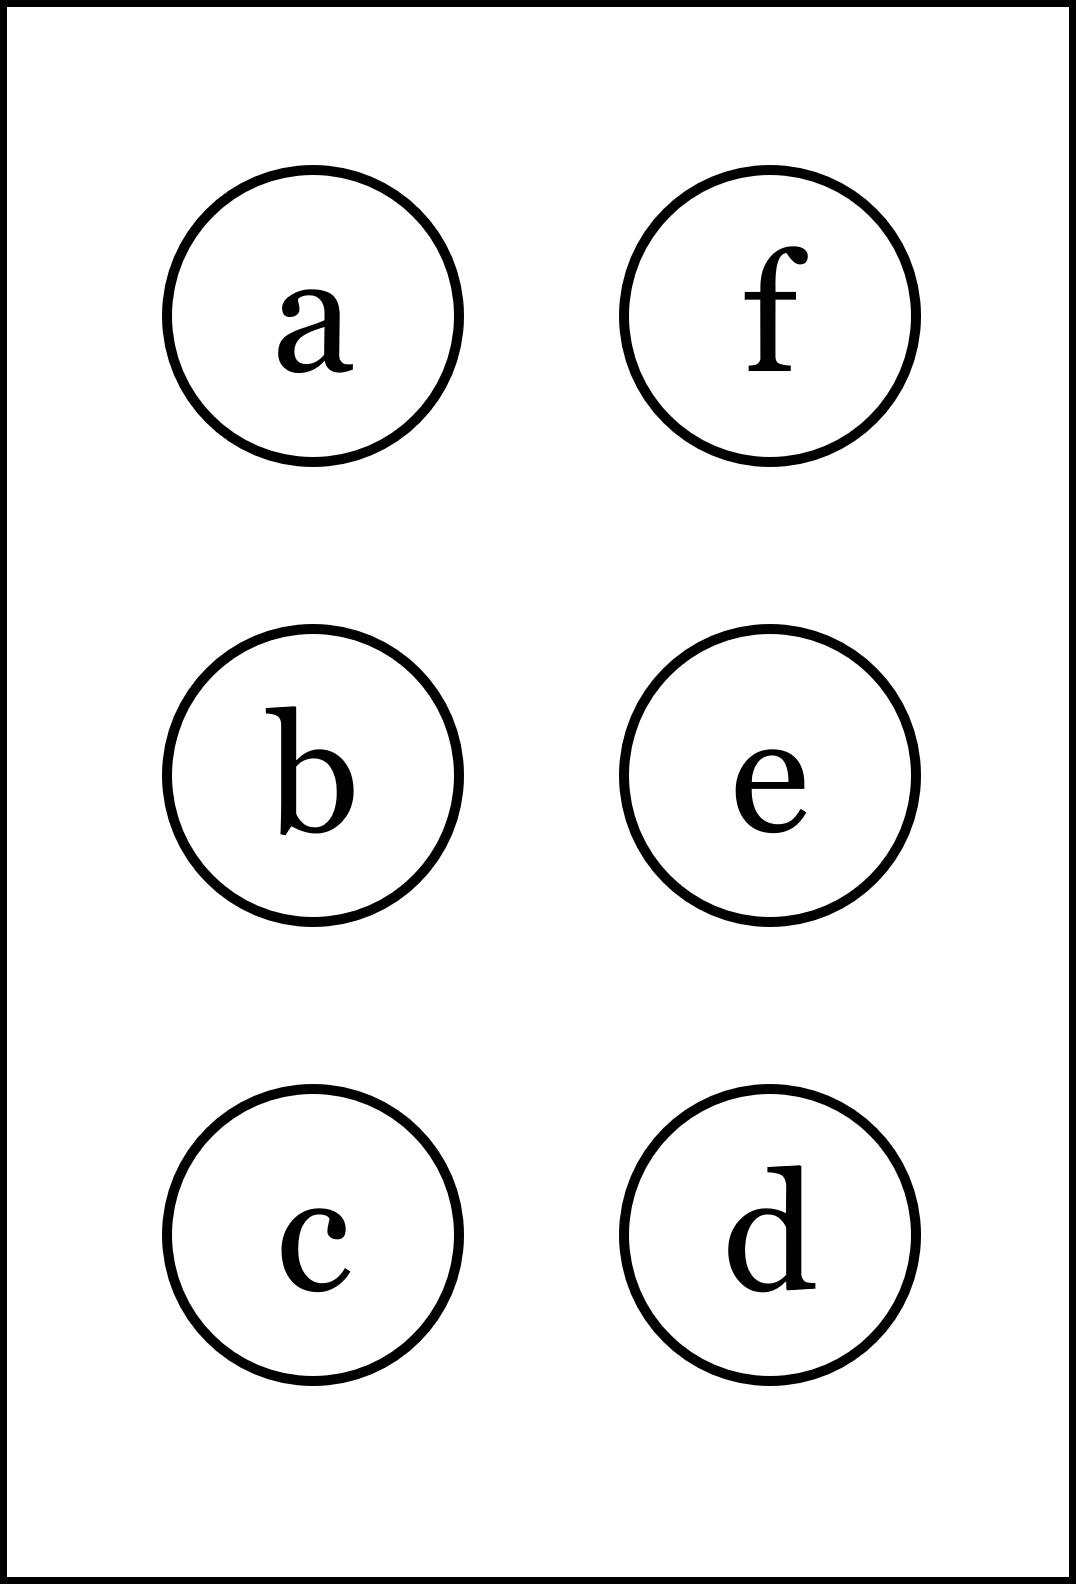
\includegraphics[height=40mm]{../images/braille.png}
{\small Písmeno Braillovej abecedy}
\end{center}
\end{minipage}
\end{center}
\end{minipage}
&
\begin{minipage}[c][99mm][t]{0.49\linewidth}
\begin{center}
\vspace{7mm}
{\huge Definiční obor, skupina \textit{Iota $\iota$} -\romannumeral4}\\[4.5mm]
\textit{Meno:}\phantom{xxxxxxxxxxxxxxxxxxxxxxxxxxxxxxxxxxxxxxxxxxxxxxxxxxxxxxxxxxxxxxxxx}\\[3.5mm]
\textbf{Zjisti definiční obor} zadaných funkcí. Pokud se shoduje s tím za otazníky,\\tak napravo obarvi příslušející kroužek načerno. \textbf{Spolu odevzdejte výsledné slovo}.\\[3mm]
\begin{minipage}{0.77\linewidth}
\begin{center}
\begin{varwidth}{\textwidth}
\begin{enumerate}
\normalsize
\item $f(x)=\cfrac{-5x-4}{-2x-3}$\quad \dotfill\; ???\;\dotfill \quad $\mathbb{R}\smallsetminus\{\nicefrac{-3}{2}\}$
\item $f(x)=\cfrac{1}{-x^3+3x+2}$\quad \dotfill\; ???\;\dotfill \quad $\mathbb{R}\smallsetminus\{0,1,2\}$
\item $f(x)=-3\sqrt{-6x-5}$\quad \dotfill\; ???\;\dotfill \quad $x\leq\nicefrac{5}{6}$
\item $f(x)=\sqrt{-x^2+7x}$\quad \dotfill\; ???\;\dotfill \quad $x\in\langle-7 , 0\rangle$
\item $f(x)=6\ln{(-x-5)}$\quad \dotfill\; ???\;\dotfill \quad $x>-5$
\item $f(x)=\ln{(x^2-5x+4)}$\quad \dotfill\; ???\;\dotfill \quad $x\in(1 , 4)$
\end{enumerate}
\end{varwidth}
\end{center}
\end{minipage}
\begin{minipage}{0.20\linewidth}
\begin{center}
{\Huge\bfseries 4.} \\[2mm]
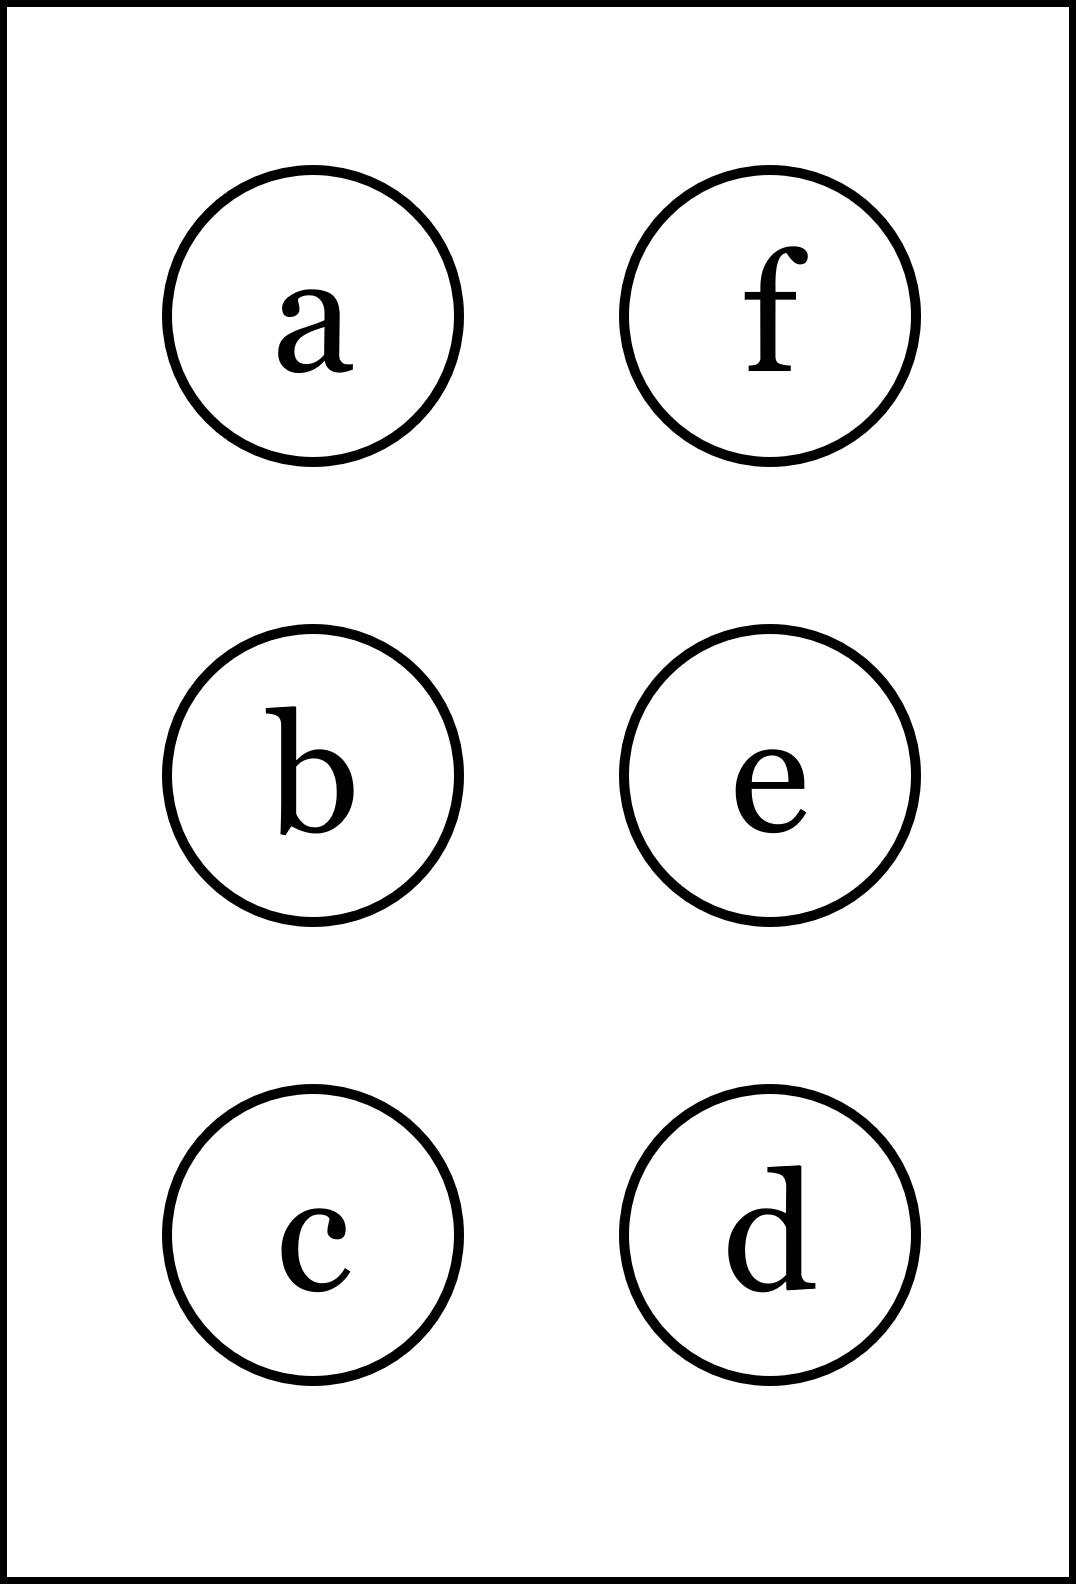
\includegraphics[height=40mm]{../images/braille.png}
{\small Písmeno Braillovej abecedy}
\end{center}
\end{minipage}
\end{center}
\end{minipage}
%
\end{tabular}
\begin{tikzpicture}[remember picture,overlay]\node[xshift=7mm,yshift=-100.6mm,anchor=north west] at (current page.north west){\ding{33}};\end{tikzpicture}
\begin{tikzpicture}[remember picture,overlay]\node[xshift=151.2mm,yshift=-7mm,anchor=north west,rotate=270] at (current page.north west){\ding{33}};\end{tikzpicture}
\newpage
\thispagestyle{empty}
\begin{tabular}{c:c}
\begin{minipage}[c][99mm][t]{0.49\linewidth}
\begin{center}
\vspace{7mm}
{\huge Definiční obor, skupina \textit{Kappa $\kappa$} -\romannumeral1}\\[4.5mm]
\textit{Meno:}\phantom{xxxxxxxxxxxxxxxxxxxxxxxxxxxxxxxxxxxxxxxxxxxxxxxxxxxxxxxxxxxxxxxxx}\\[3.5mm]
\textbf{Zjisti definiční obor} zadaných funkcí. Pokud se shoduje s tím za otazníky,\\tak napravo obarvi příslušející kroužek načerno. \textbf{Spolu odevzdejte výsledné slovo}.\\[3mm]
\begin{minipage}{0.77\linewidth}
\begin{center}
\begin{varwidth}{\textwidth}
\begin{enumerate}
\normalsize
\item $f(x)=\cfrac{-x+6}{-9x+1}$\quad \dotfill\; ???\;\dotfill \quad $\mathbb{R}\smallsetminus\{\nicefrac{1}{9}\}$
\item $f(x)=\cfrac{1}{-x^3+3x^2+4x-12}$\quad \dotfill\; ???\;\dotfill \quad $\mathbb{R}\smallsetminus\{2,3,-2\}$
\item $f(x)=1\sqrt{-7x-1}$\quad \dotfill\; ???\;\dotfill \quad $x\geq\nicefrac{-1}{7}$
\item $f(x)=\sqrt{-x^2+5x}$\quad \dotfill\; ???\;\dotfill \quad $x\in\langle-5 , 0\rangle$
\item $f(x)=-3\ln{(-x+1)}$\quad \dotfill\; ???\;\dotfill \quad $x<-1$
\item $f(x)=\ln{(x^2-1)}$\quad \dotfill\; ???\;\dotfill \quad $x\in(-\infty , -1)\cup(1 , \infty)$
\end{enumerate}
\end{varwidth}
\end{center}
\end{minipage}
\begin{minipage}{0.20\linewidth}
\begin{center}
{\Huge\bfseries 1.} \\[2mm]
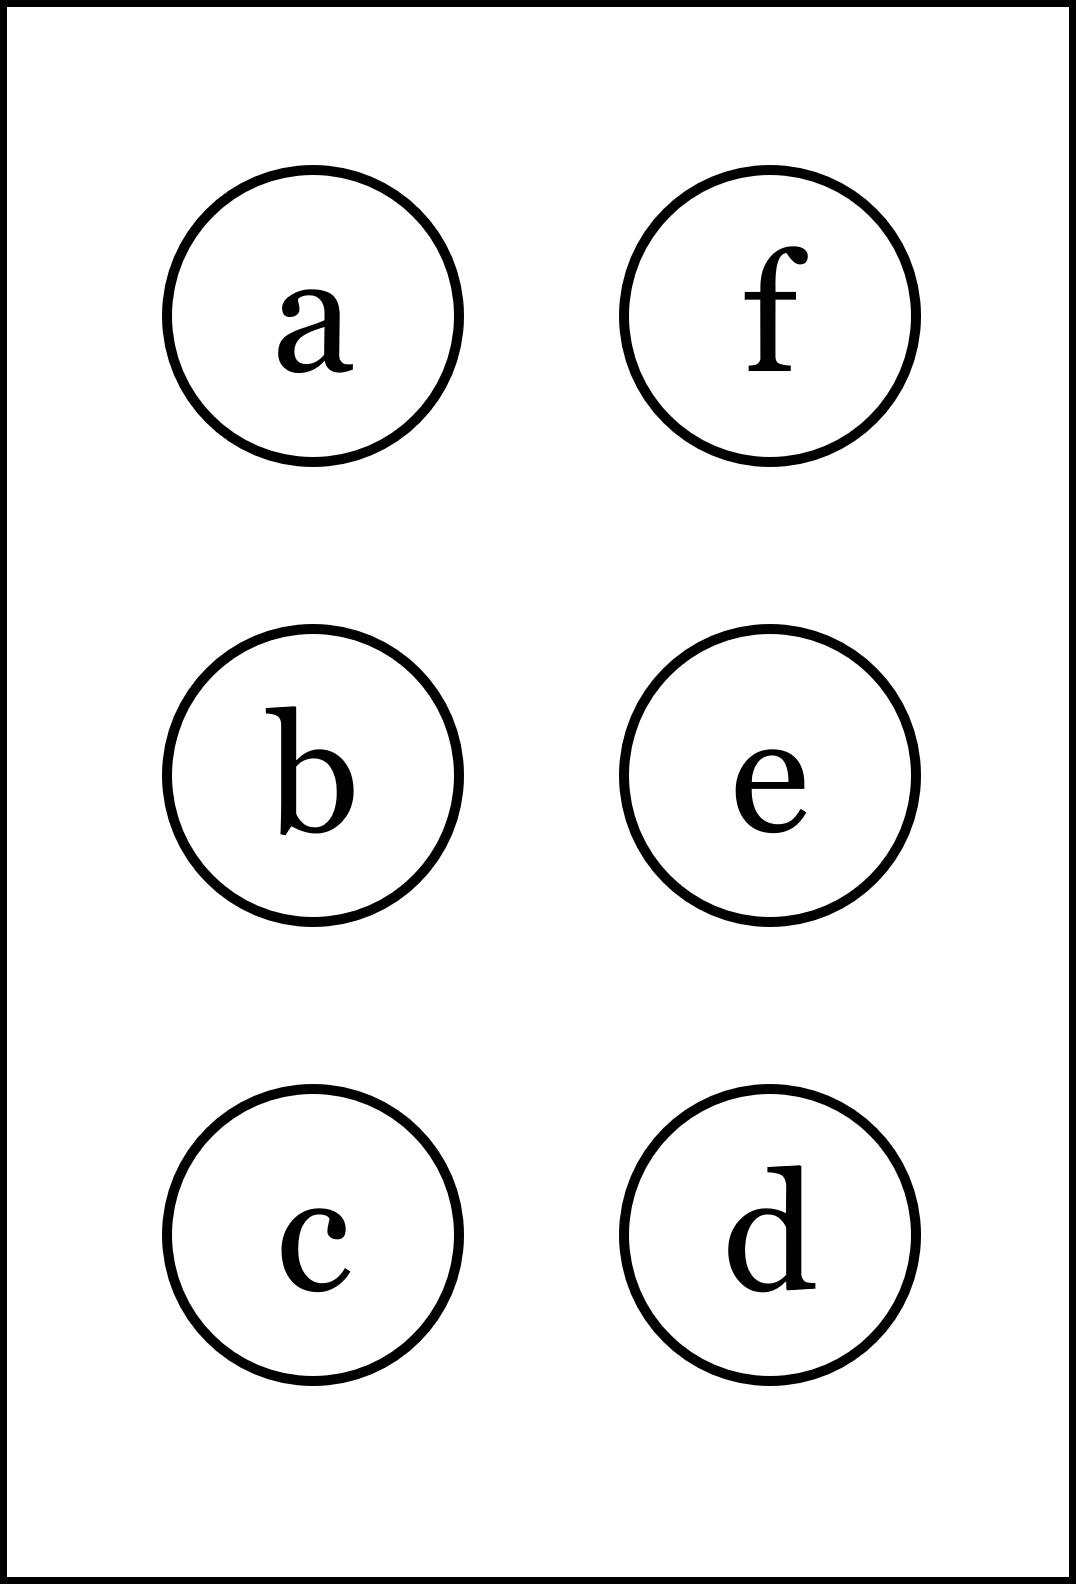
\includegraphics[height=40mm]{../images/braille.png}
{\small Písmeno Braillovej abecedy}
\end{center}
\end{minipage}
\end{center}
\end{minipage}
&
\begin{minipage}[c][99mm][t]{0.49\linewidth}
\begin{center}
\vspace{7mm}
{\huge Definiční obor, skupina \textit{Kappa $\kappa$} -\romannumeral2}\\[4.5mm]
\textit{Meno:}\phantom{xxxxxxxxxxxxxxxxxxxxxxxxxxxxxxxxxxxxxxxxxxxxxxxxxxxxxxxxxxxxxxxxx}\\[3.5mm]
\textbf{Zjisti definiční obor} zadaných funkcí. Pokud se shoduje s tím za otazníky,\\tak napravo obarvi příslušející kroužek načerno. \textbf{Spolu odevzdejte výsledné slovo}.\\[3mm]
\begin{minipage}{0.77\linewidth}
\begin{center}
\begin{varwidth}{\textwidth}
\begin{enumerate}
\normalsize
\item $f(x)=\cfrac{2x-3}{-5x+9}$\quad \dotfill\; ???\;\dotfill \quad $\mathbb{R}\smallsetminus\{\nicefrac{9}{5}\}$
\item $f(x)=\cfrac{1}{x^3-4x^2-15x+18}$\quad \dotfill\; ???\;\dotfill \quad $\mathbb{R}\smallsetminus\{1,-6,-1\}$
\item $f(x)=-4\sqrt{-5x+7}$\quad \dotfill\; ???\;\dotfill \quad $x\geq\nicefrac{7}{5}$
\item $f(x)=\sqrt{-x^2-2x}$\quad \dotfill\; ???\;\dotfill \quad $x\in(-2 , 0)$
\item $f(x)=6\ln{(6x-8)}$\quad \dotfill\; ???\;\dotfill \quad $x>\nicefrac{4}{3}$
\item $f(x)=\ln{(x^2-3x-18)}$\quad \dotfill\; ???\;\dotfill \quad $x\in(-3 , 6)$
\end{enumerate}
\end{varwidth}
\end{center}
\end{minipage}
\begin{minipage}{0.20\linewidth}
\begin{center}
{\Huge\bfseries 2.} \\[2mm]
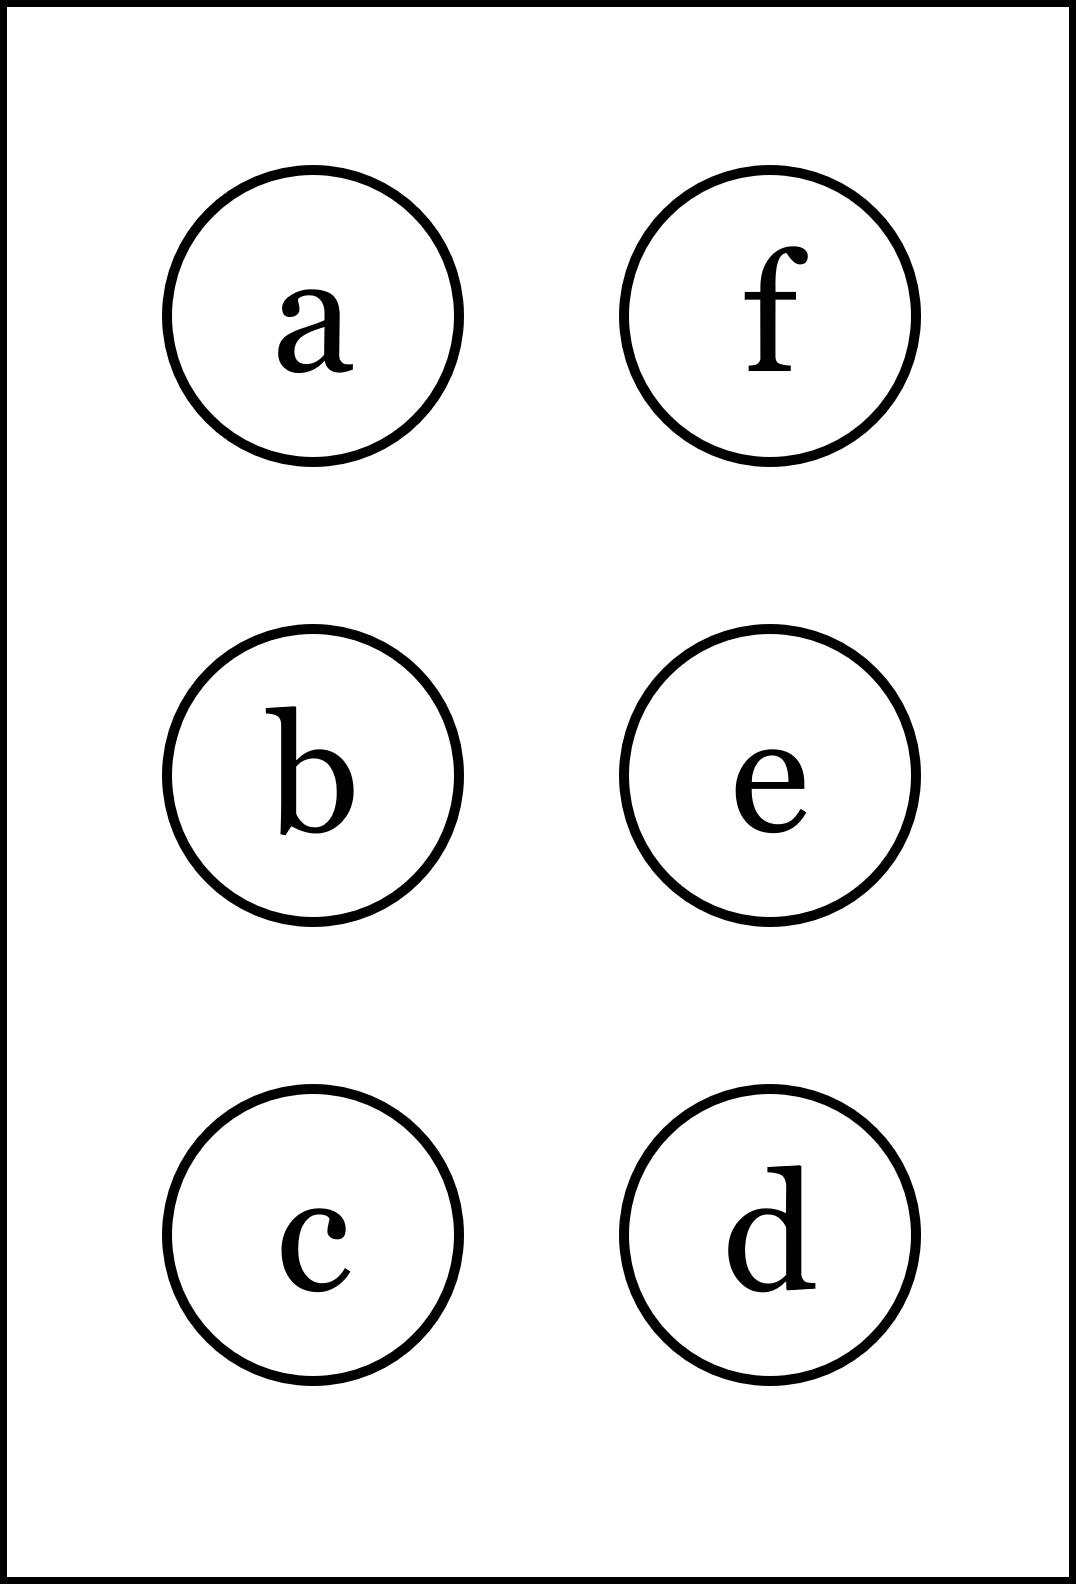
\includegraphics[height=40mm]{../images/braille.png}
{\small Písmeno Braillovej abecedy}
\end{center}
\end{minipage}
\end{center}
\end{minipage}
\\ \hdashline
\begin{minipage}[c][99mm][t]{0.49\linewidth}
\begin{center}
\vspace{7mm}
{\huge Definiční obor, skupina \textit{Kappa $\kappa$} -\romannumeral3}\\[4.5mm]
\textit{Meno:}\phantom{xxxxxxxxxxxxxxxxxxxxxxxxxxxxxxxxxxxxxxxxxxxxxxxxxxxxxxxxxxxxxxxxx}\\[3.5mm]
\textbf{Zjisti definiční obor} zadaných funkcí. Pokud se shoduje s tím za otazníky,\\tak napravo obarvi příslušející kroužek načerno. \textbf{Spolu odevzdejte výsledné slovo}.\\[3mm]
\begin{minipage}{0.77\linewidth}
\begin{center}
\begin{varwidth}{\textwidth}
\begin{enumerate}
\normalsize
\item $f(x)=\cfrac{-7x-1}{2x+3}$\quad \dotfill\; ???\;\dotfill \quad $\mathbb{R}\smallsetminus\{\nicefrac{-3}{2}\}$
\item $f(x)=\cfrac{1}{4x^3+16x^2+20x+8}$\quad \dotfill\; ???\;\dotfill \quad $\mathbb{R}\smallsetminus\{1,2,-1\}$
\item $f(x)=-3\sqrt{-3x+5}$\quad \dotfill\; ???\;\dotfill \quad $x\leq\nicefrac{5}{3}$
\item $f(x)=\sqrt{-x^2-4x}$\quad \dotfill\; ???\;\dotfill \quad $x\in\langle0 , 4\rangle$
\item $f(x)=-2\ln{(-x-6)}$\quad \dotfill\; ???\;\dotfill \quad $x<-6$
\item $f(x)=\ln{(x^2+9x+8)}$\quad \dotfill\; ???\;\dotfill \quad $x\in(-\infty , -8)\cup(-1 , \infty)$
\end{enumerate}
\end{varwidth}
\end{center}
\end{minipage}
\begin{minipage}{0.20\linewidth}
\begin{center}
{\Huge\bfseries 3.} \\[2mm]
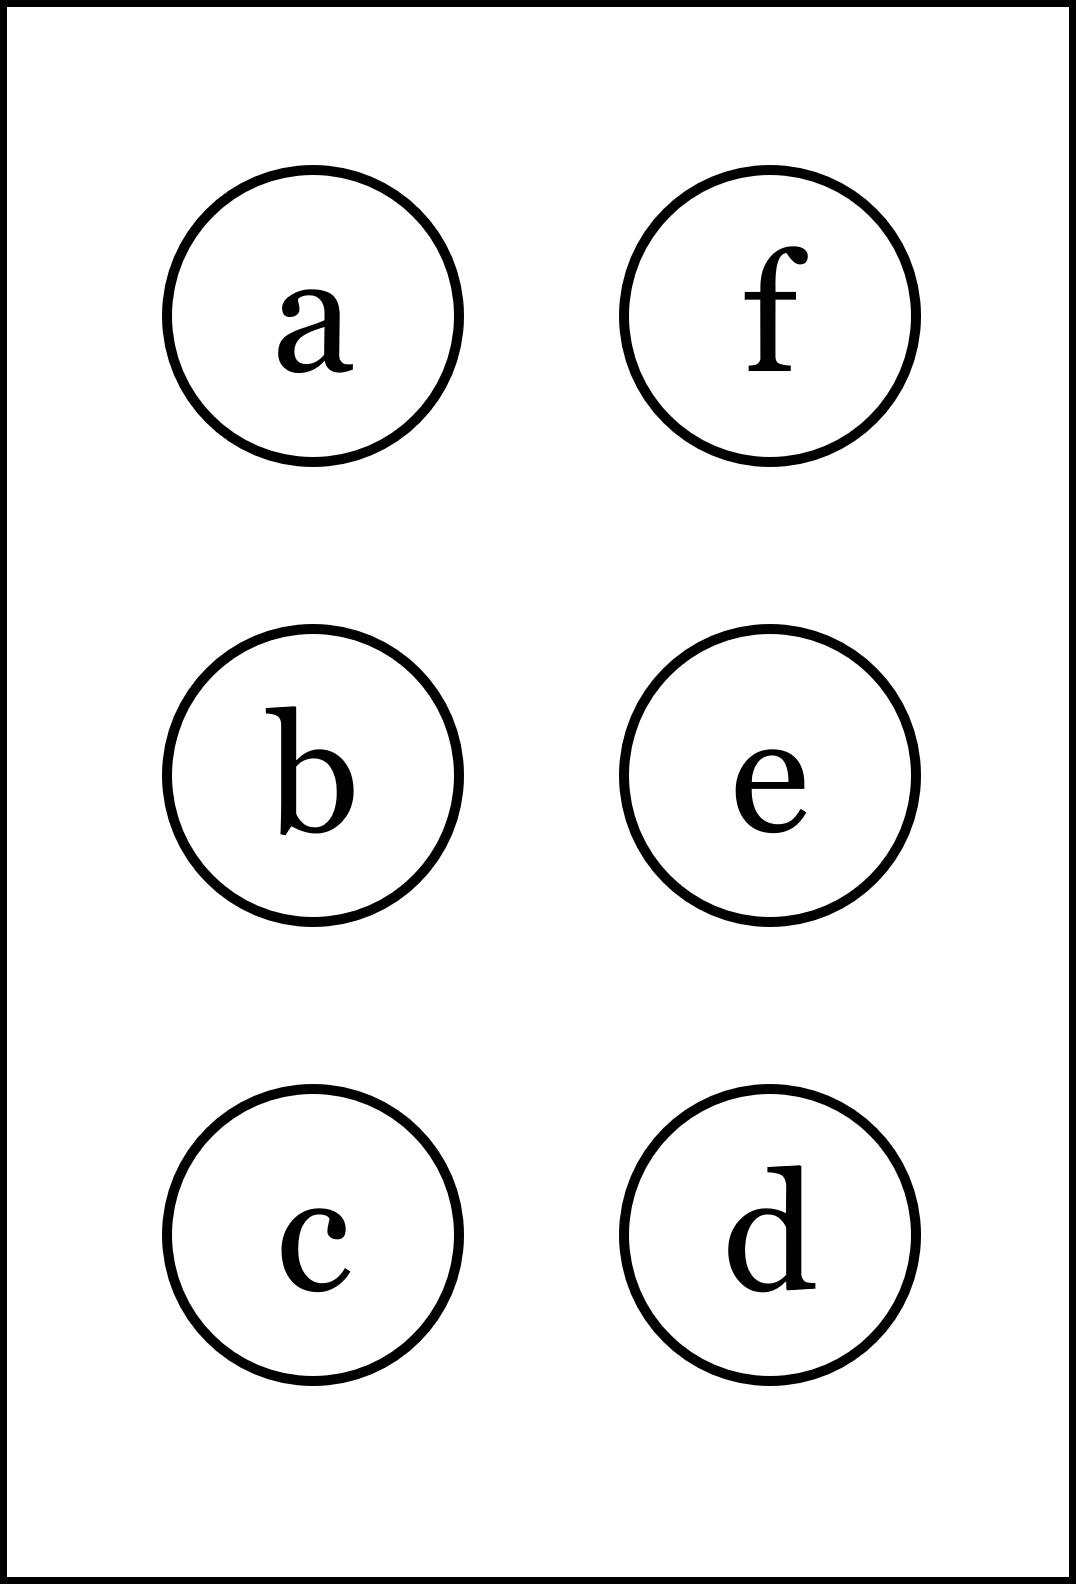
\includegraphics[height=40mm]{../images/braille.png}
{\small Písmeno Braillovej abecedy}
\end{center}
\end{minipage}
\end{center}
\end{minipage}
&
\begin{minipage}[c][99mm][t]{0.49\linewidth}
\begin{center}
\vspace{7mm}
{\huge Definiční obor, skupina \textit{Kappa $\kappa$} -\romannumeral4}\\[4.5mm]
\textit{Meno:}\phantom{xxxxxxxxxxxxxxxxxxxxxxxxxxxxxxxxxxxxxxxxxxxxxxxxxxxxxxxxxxxxxxxxx}\\[3.5mm]
\textbf{Zjisti definiční obor} zadaných funkcí. Pokud se shoduje s tím za otazníky,\\tak napravo obarvi příslušející kroužek načerno. \textbf{Spolu odevzdejte výsledné slovo}.\\[3mm]
\begin{minipage}{0.77\linewidth}
\begin{center}
\begin{varwidth}{\textwidth}
\begin{enumerate}
\normalsize
\item $f(x)=\cfrac{2x-6}{-7x+5}$\quad \dotfill\; ???\;\dotfill \quad $\mathbb{R}\smallsetminus\{\nicefrac{5}{7}\}$
\item $f(x)=\cfrac{1}{-4x^3+12x^2+52x-60}$\quad \dotfill\; ???\;\dotfill \quad $\mathbb{R}\smallsetminus\{-5,5,-1\}$
\item $f(x)=-6\sqrt{-x+3}$\quad \dotfill\; ???\;\dotfill \quad $x\leq-3$
\item $f(x)=\sqrt{-x^2+x}$\quad \dotfill\; ???\;\dotfill \quad $x\in(0 , 1)$
\item $f(x)=9\ln{(x+3)}$\quad \dotfill\; ???\;\dotfill \quad $x<-3$
\item $f(x)=\ln{(x^2+6x+5)}$\quad \dotfill\; ???\;\dotfill \quad $x\in(-5 , -1)$
\end{enumerate}
\end{varwidth}
\end{center}
\end{minipage}
\begin{minipage}{0.20\linewidth}
\begin{center}
{\Huge\bfseries 4.} \\[2mm]
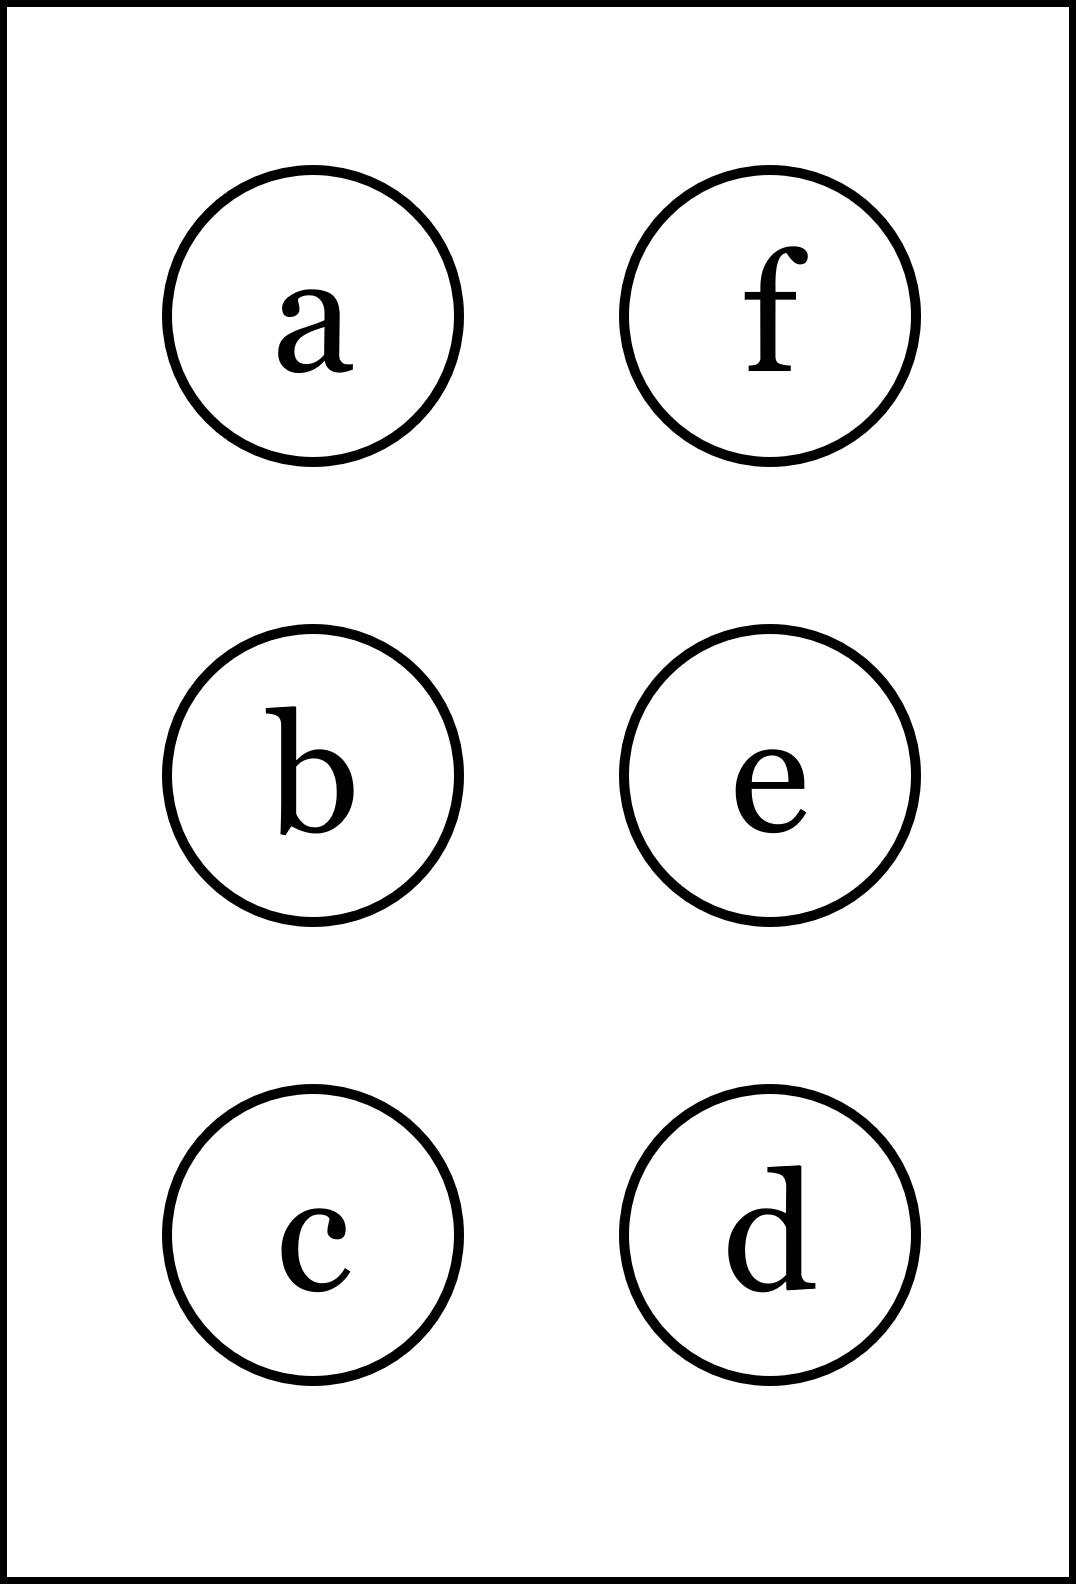
\includegraphics[height=40mm]{../images/braille.png}
{\small Písmeno Braillovej abecedy}
\end{center}
\end{minipage}
\end{center}
\end{minipage}
%
\end{tabular}
\begin{tikzpicture}[remember picture,overlay]\node[xshift=7mm,yshift=-100.6mm,anchor=north west] at (current page.north west){\ding{33}};\end{tikzpicture}
\begin{tikzpicture}[remember picture,overlay]\node[xshift=151.2mm,yshift=-7mm,anchor=north west,rotate=270] at (current page.north west){\ding{33}};\end{tikzpicture}
\newpage
\thispagestyle{empty}
\begin{tabular}{c:c}
\begin{minipage}[c][99mm][t]{0.49\linewidth}
\begin{center}
\vspace{7mm}
{\huge Definiční obor, skupina \textit{Lambda $\lambda$} -\romannumeral1}\\[4.5mm]
\textit{Meno:}\phantom{xxxxxxxxxxxxxxxxxxxxxxxxxxxxxxxxxxxxxxxxxxxxxxxxxxxxxxxxxxxxxxxxx}\\[3.5mm]
\textbf{Zjisti definiční obor} zadaných funkcí. Pokud se shoduje s tím za otazníky,\\tak napravo obarvi příslušející kroužek načerno. \textbf{Spolu odevzdejte výsledné slovo}.\\[3mm]
\begin{minipage}{0.77\linewidth}
\begin{center}
\begin{varwidth}{\textwidth}
\begin{enumerate}
\normalsize
\item $f(x)=\cfrac{-8x+7}{2x-3}$\quad \dotfill\; ???\;\dotfill \quad $\mathbb{R}\smallsetminus\{\nicefrac{3}{2}\}$
\item $f(x)=\cfrac{1}{-3x^3+24x^2+3x-24}$\quad \dotfill\; ???\;\dotfill \quad $\mathbb{R}\smallsetminus\{0,-8,-1\}$
\item $f(x)=6\sqrt{-4x+4}$\quad \dotfill\; ???\;\dotfill \quad $x\leq-1$
\item $f(x)=\sqrt{-x^2-6x}$\quad \dotfill\; ???\;\dotfill \quad $x\in(-6 , 0)$
\item $f(x)=2\ln{(2x+1)}$\quad \dotfill\; ???\;\dotfill \quad $x>\nicefrac{-1}{2}$
\item $f(x)=\ln{(x^2+2x-24)}$\quad \dotfill\; ???\;\dotfill \quad $x\in(-\infty , -6)\cup(4 , \infty)$
\end{enumerate}
\end{varwidth}
\end{center}
\end{minipage}
\begin{minipage}{0.20\linewidth}
\begin{center}
{\Huge\bfseries 1.} \\[2mm]
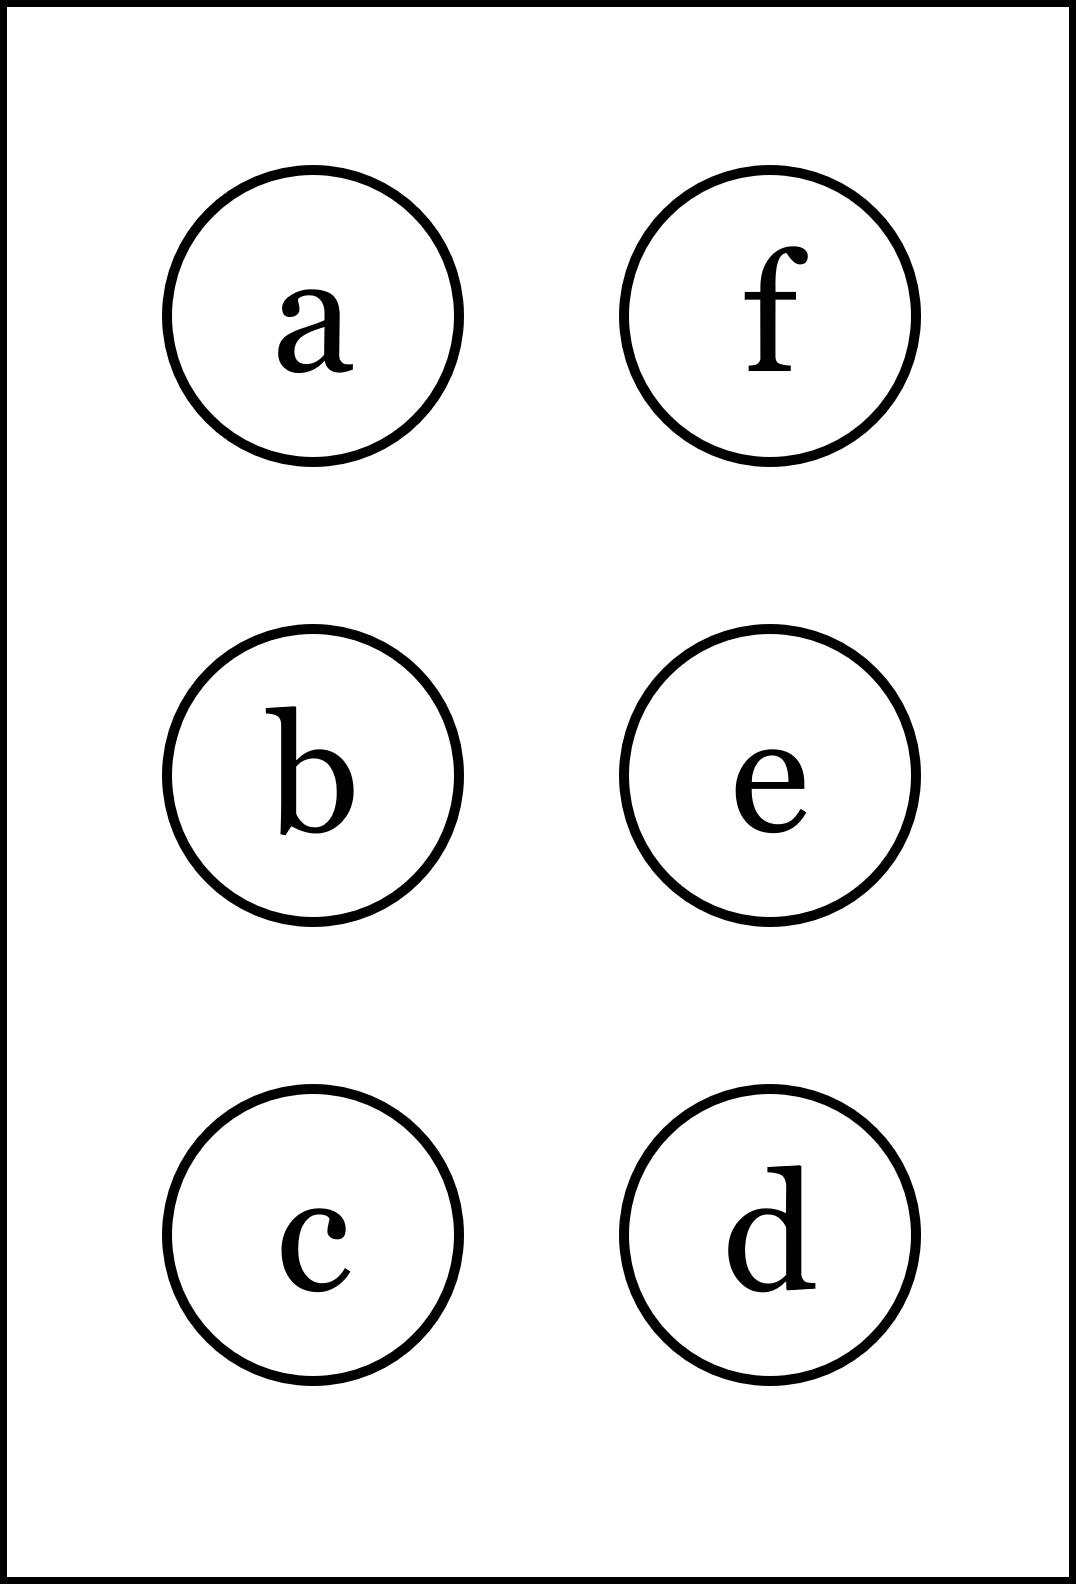
\includegraphics[height=40mm]{../images/braille.png}
{\small Písmeno Braillovej abecedy}
\end{center}
\end{minipage}
\end{center}
\end{minipage}
&
\begin{minipage}[c][99mm][t]{0.49\linewidth}
\begin{center}
\vspace{7mm}
{\huge Definiční obor, skupina \textit{Lambda $\lambda$} -\romannumeral2}\\[4.5mm]
\textit{Meno:}\phantom{xxxxxxxxxxxxxxxxxxxxxxxxxxxxxxxxxxxxxxxxxxxxxxxxxxxxxxxxxxxxxxxxx}\\[3.5mm]
\textbf{Zjisti definiční obor} zadaných funkcí. Pokud se shoduje s tím za otazníky,\\tak napravo obarvi příslušející kroužek načerno. \textbf{Spolu odevzdejte výsledné slovo}.\\[3mm]
\begin{minipage}{0.77\linewidth}
\begin{center}
\begin{varwidth}{\textwidth}
\begin{enumerate}
\normalsize
\item $f(x)=\cfrac{x-1}{-7x-2}$\quad \dotfill\; ???\;\dotfill \quad $\mathbb{R}\smallsetminus\{\nicefrac{-2}{7}\}$
\item $f(x)=\cfrac{1}{-2x^3+14x+12}$\quad \dotfill\; ???\;\dotfill \quad $\mathbb{R}\smallsetminus\{1,5,-2\}$
\item $f(x)=-4\sqrt{-5x+2}$\quad \dotfill\; ???\;\dotfill \quad $x\leq\nicefrac{2}{5}$
\item $f(x)=\sqrt{-x^2+5x}$\quad \dotfill\; ???\;\dotfill \quad $x\in(0 , 5)$
\item $f(x)=-8\ln{(-2x+5)}$\quad \dotfill\; ???\;\dotfill \quad $x<\nicefrac{5}{2}$
\item $f(x)=\ln{(x^2+x-20)}$\quad \dotfill\; ???\;\dotfill \quad $x\in(-5 , 4)$
\end{enumerate}
\end{varwidth}
\end{center}
\end{minipage}
\begin{minipage}{0.20\linewidth}
\begin{center}
{\Huge\bfseries 2.} \\[2mm]
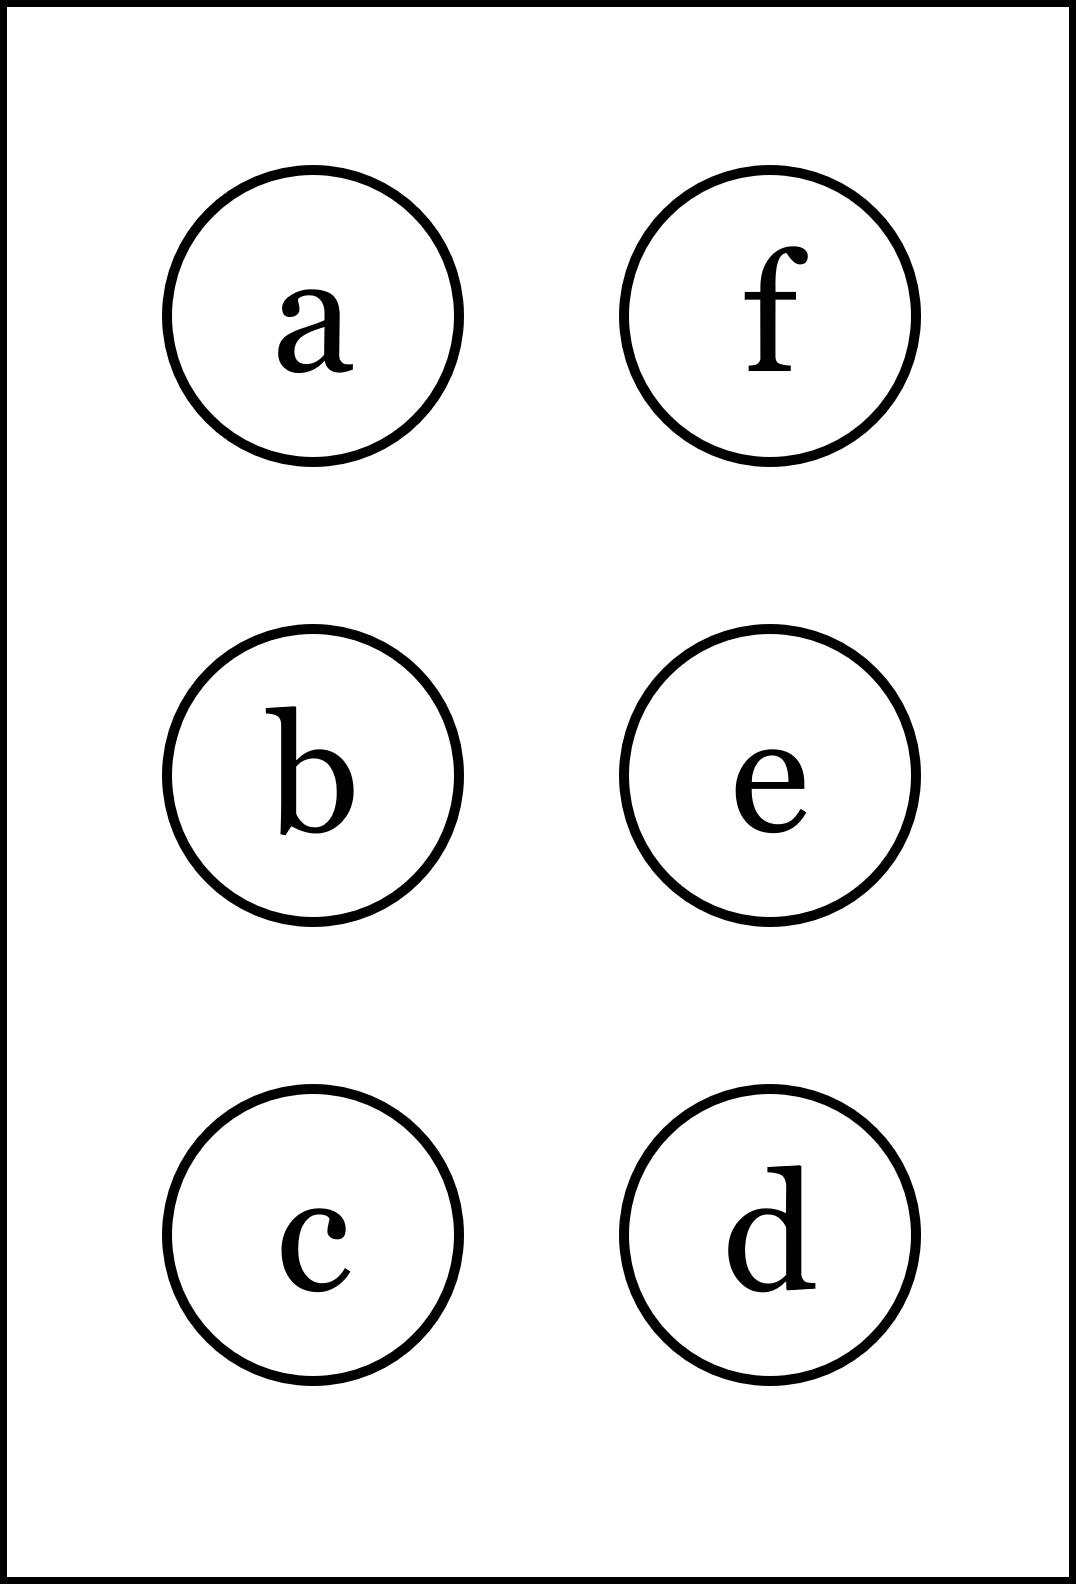
\includegraphics[height=40mm]{../images/braille.png}
{\small Písmeno Braillovej abecedy}
\end{center}
\end{minipage}
\end{center}
\end{minipage}
\\ \hdashline
\begin{minipage}[c][99mm][t]{0.49\linewidth}
\begin{center}
\vspace{7mm}
{\huge Definiční obor, skupina \textit{Lambda $\lambda$} -\romannumeral3}\\[4.5mm]
\textit{Meno:}\phantom{xxxxxxxxxxxxxxxxxxxxxxxxxxxxxxxxxxxxxxxxxxxxxxxxxxxxxxxxxxxxxxxxx}\\[3.5mm]
\textbf{Zjisti definiční obor} zadaných funkcí. Pokud se shoduje s tím za otazníky,\\tak napravo obarvi příslušející kroužek načerno. \textbf{Spolu odevzdejte výsledné slovo}.\\[3mm]
\begin{minipage}{0.77\linewidth}
\begin{center}
\begin{varwidth}{\textwidth}
\begin{enumerate}
\normalsize
\item $f(x)=\cfrac{-2x+1}{-8x-5}$\quad \dotfill\; ???\;\dotfill \quad $\mathbb{R}\smallsetminus\{\nicefrac{-5}{8}\}$
\item $f(x)=\cfrac{1}{x^3-8x^2+21x-18}$\quad \dotfill\; ???\;\dotfill \quad $\mathbb{R}\smallsetminus\{3,5,-2\}$
\item $f(x)=6\sqrt{x-8}$\quad \dotfill\; ???\;\dotfill \quad $x\geq8$
\item $f(x)=\sqrt{-x^2+3x}$\quad \dotfill\; ???\;\dotfill \quad $x\in\langle-3 , 0\rangle$
\item $f(x)=1\ln{(x-1)}$\quad \dotfill\; ???\;\dotfill \quad $x>-1$
\item $f(x)=\ln{(x^2+5x-14)}$\quad \dotfill\; ???\;\dotfill \quad $x\in(-\infty , -7)\cup(2 , \infty)$
\end{enumerate}
\end{varwidth}
\end{center}
\end{minipage}
\begin{minipage}{0.20\linewidth}
\begin{center}
{\Huge\bfseries 3.} \\[2mm]
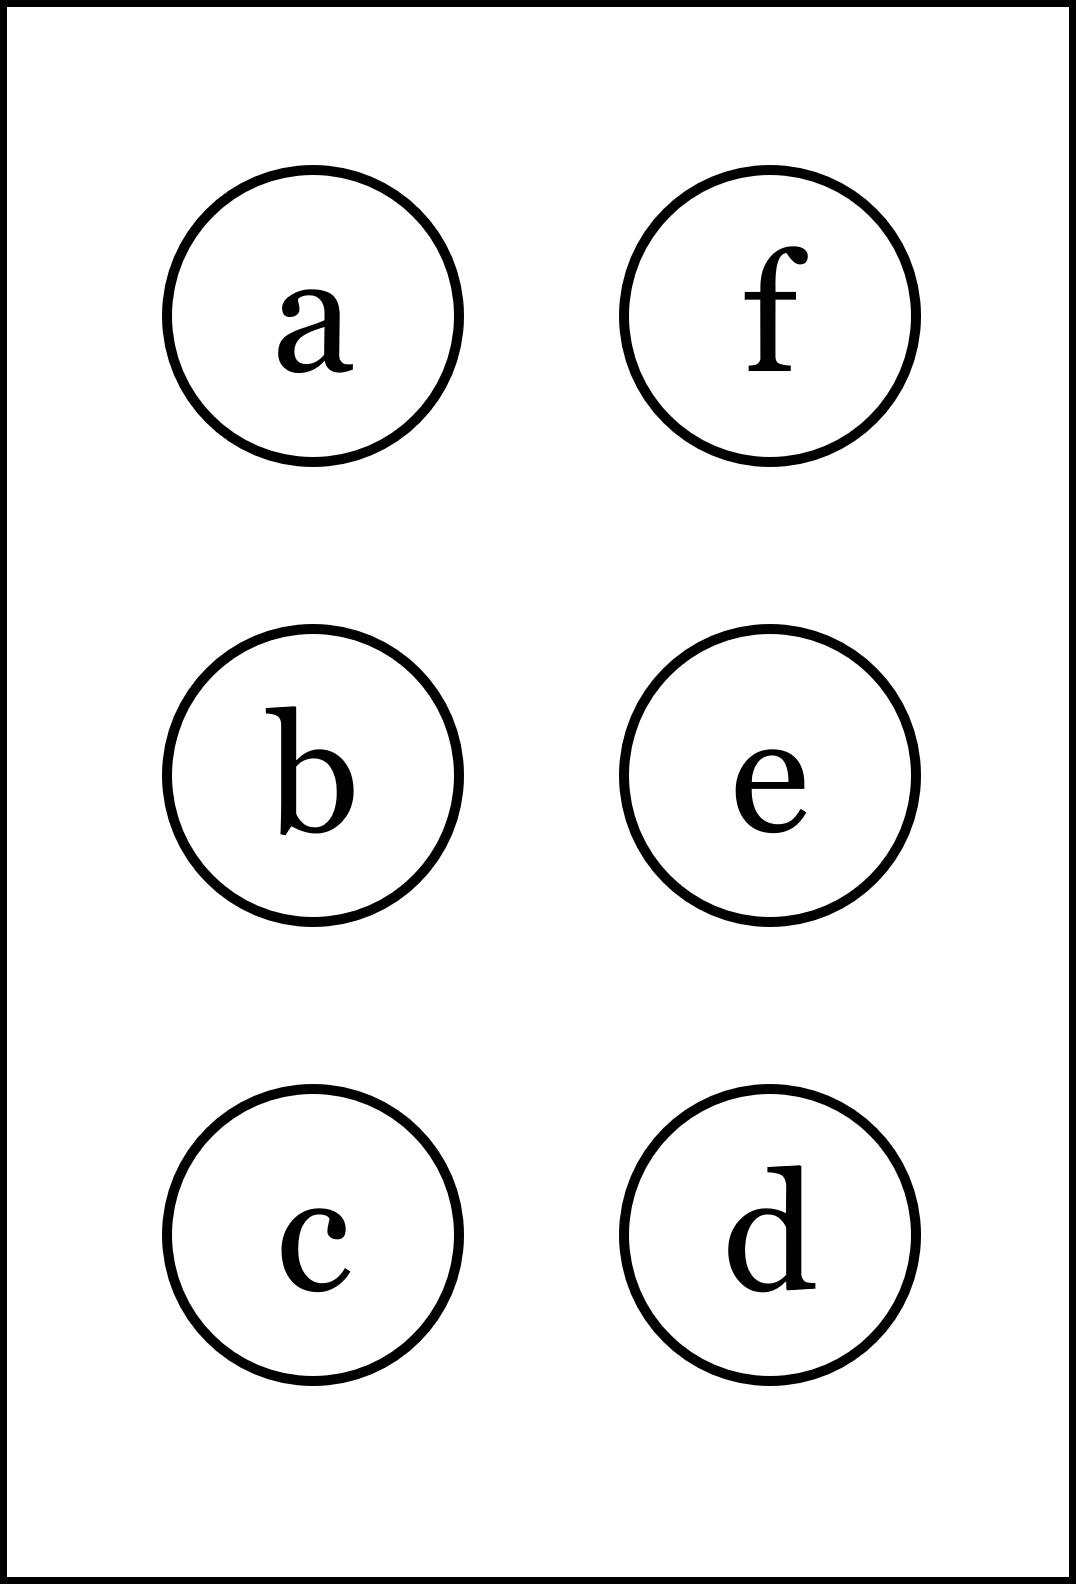
\includegraphics[height=40mm]{../images/braille.png}
{\small Písmeno Braillovej abecedy}
\end{center}
\end{minipage}
\end{center}
\end{minipage}
&
\begin{minipage}[c][99mm][t]{0.49\linewidth}
\begin{center}
\vspace{7mm}
{\huge Definiční obor, skupina \textit{Lambda $\lambda$} -\romannumeral4}\\[4.5mm]
\textit{Meno:}\phantom{xxxxxxxxxxxxxxxxxxxxxxxxxxxxxxxxxxxxxxxxxxxxxxxxxxxxxxxxxxxxxxxxx}\\[3.5mm]
\textbf{Zjisti definiční obor} zadaných funkcí. Pokud se shoduje s tím za otazníky,\\tak napravo obarvi příslušející kroužek načerno. \textbf{Spolu odevzdejte výsledné slovo}.\\[3mm]
\begin{minipage}{0.77\linewidth}
\begin{center}
\begin{varwidth}{\textwidth}
\begin{enumerate}
\normalsize
\item $f(x)=\cfrac{-2x+8}{-2x-4}$\quad \dotfill\; ???\;\dotfill \quad $\mathbb{R}\smallsetminus\{-2\}$
\item $f(x)=\cfrac{1}{4x^3+28x^2+56x+32}$\quad \dotfill\; ???\;\dotfill \quad $\mathbb{R}\smallsetminus\{1,-3,-2\}$
\item $f(x)=6\sqrt{x-1}$\quad \dotfill\; ???\;\dotfill \quad $x\leq1$
\item $f(x)=\sqrt{-x^2-2x}$\quad \dotfill\; ???\;\dotfill \quad $x\in(-2 , 0)$
\item $f(x)=-1\ln{(6x+1)}$\quad \dotfill\; ???\;\dotfill \quad $x<\nicefrac{-1}{6}$
\item $f(x)=\ln{(x^2+x-12)}$\quad \dotfill\; ???\;\dotfill \quad $x\in(-4 , 3)$
\end{enumerate}
\end{varwidth}
\end{center}
\end{minipage}
\begin{minipage}{0.20\linewidth}
\begin{center}
{\Huge\bfseries 4.} \\[2mm]
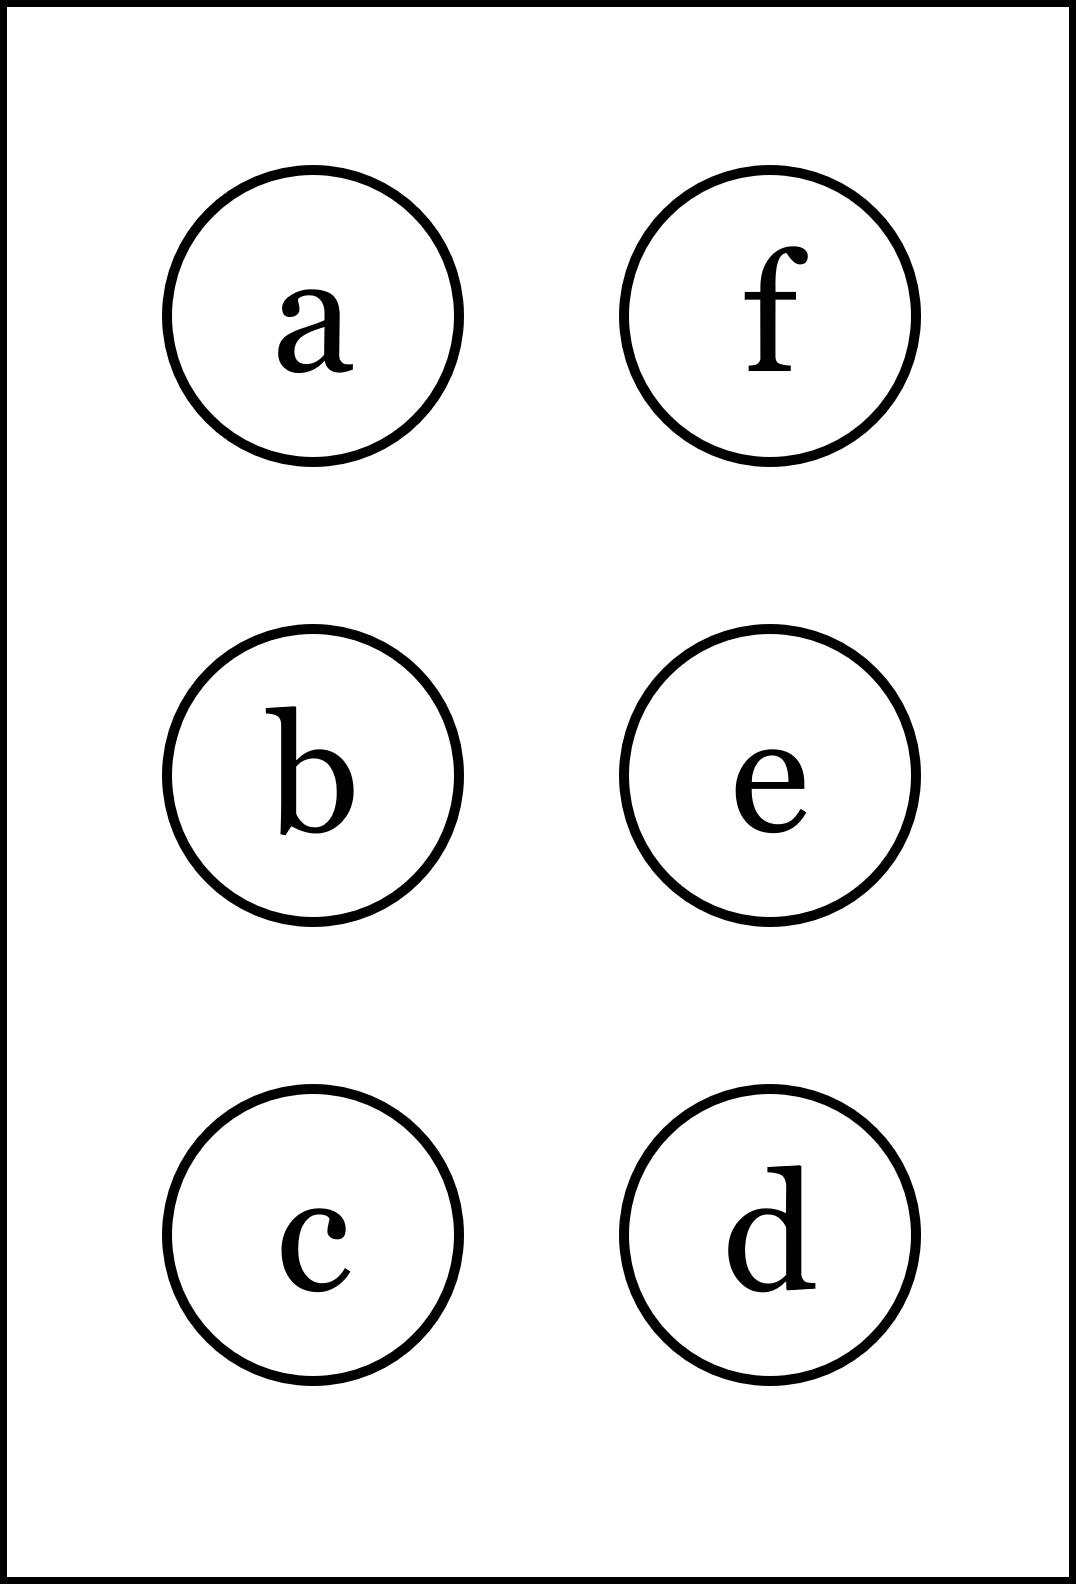
\includegraphics[height=40mm]{../images/braille.png}
{\small Písmeno Braillovej abecedy}
\end{center}
\end{minipage}
\end{center}
\end{minipage}
%
\end{tabular}
\begin{tikzpicture}[remember picture,overlay]\node[xshift=7mm,yshift=-100.6mm,anchor=north west] at (current page.north west){\ding{33}};\end{tikzpicture}
\begin{tikzpicture}[remember picture,overlay]\node[xshift=151.2mm,yshift=-7mm,anchor=north west,rotate=270] at (current page.north west){\ding{33}};\end{tikzpicture}
\newpage
\thispagestyle{empty}
\begin{tabular}{c:c}
\begin{minipage}[c][99mm][t]{0.49\linewidth}
\begin{center}
\vspace{7mm}
{\huge Definiční obor, skupina \textit{Mu $\mu$} -\romannumeral1}\\[4.5mm]
\textit{Meno:}\phantom{xxxxxxxxxxxxxxxxxxxxxxxxxxxxxxxxxxxxxxxxxxxxxxxxxxxxxxxxxxxxxxxxx}\\[3.5mm]
\textbf{Zjisti definiční obor} zadaných funkcí. Pokud se shoduje s tím za otazníky,\\tak napravo obarvi příslušející kroužek načerno. \textbf{Spolu odevzdejte výsledné slovo}.\\[3mm]
\begin{minipage}{0.77\linewidth}
\begin{center}
\begin{varwidth}{\textwidth}
\begin{enumerate}
\normalsize
\item $f(x)=\cfrac{3x+3}{2x+3}$\quad \dotfill\; ???\;\dotfill \quad $\mathbb{R}\smallsetminus\{\nicefrac{-3}{2}\}$
\item $f(x)=\cfrac{1}{-x^3+8x^2-13x+6}$\quad \dotfill\; ???\;\dotfill \quad $\mathbb{R}\smallsetminus\{1,6\}$
\item $f(x)=-5\sqrt{-3x+6}$\quad \dotfill\; ???\;\dotfill \quad $x\leq2$
\item $f(x)=\sqrt{-x^2-2x}$\quad \dotfill\; ???\;\dotfill \quad $x\in\langle0 , 2\rangle$
\item $f(x)=1\ln{(-6x-1)}$\quad \dotfill\; ???\;\dotfill \quad $x<\nicefrac{-1}{6}$
\item $f(x)=\ln{(x^2-4)}$\quad \dotfill\; ???\;\dotfill \quad $x\in(-2 , 2)$
\end{enumerate}
\end{varwidth}
\end{center}
\end{minipage}
\begin{minipage}{0.20\linewidth}
\begin{center}
{\Huge\bfseries 1.} \\[2mm]
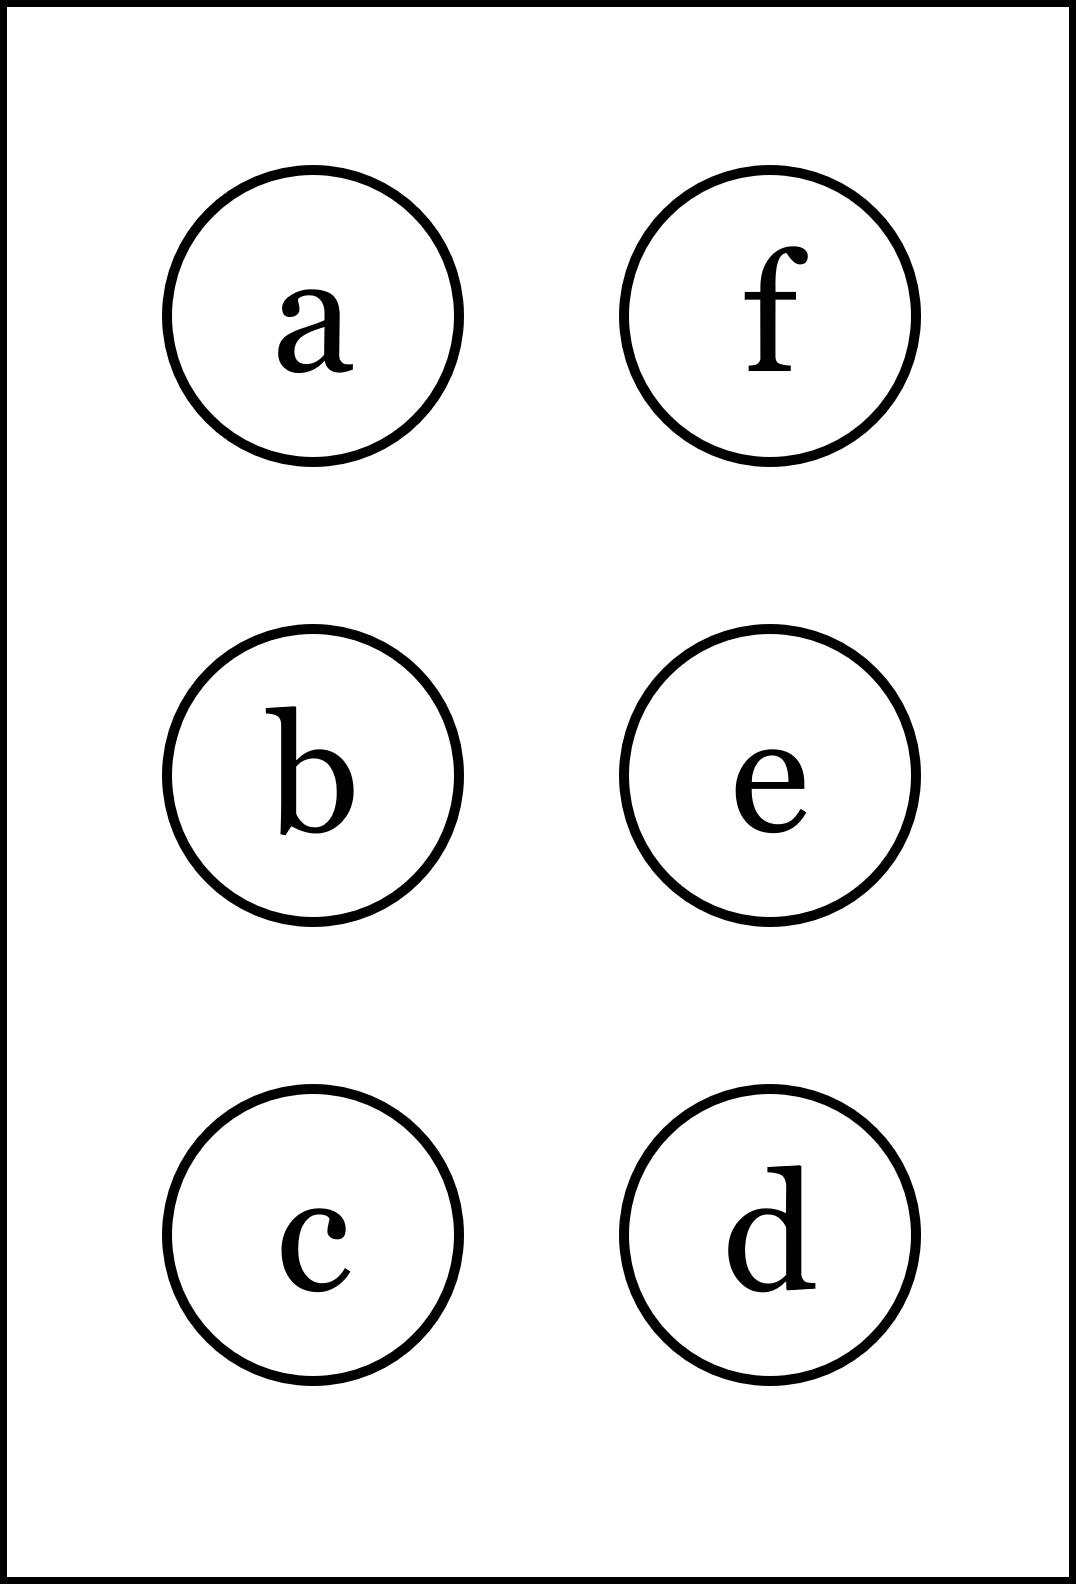
\includegraphics[height=40mm]{../images/braille.png}
{\small Písmeno Braillovej abecedy}
\end{center}
\end{minipage}
\end{center}
\end{minipage}
&
\begin{minipage}[c][99mm][t]{0.49\linewidth}
\begin{center}
\vspace{7mm}
{\huge Definiční obor, skupina \textit{Mu $\mu$} -\romannumeral2}\\[4.5mm]
\textit{Meno:}\phantom{xxxxxxxxxxxxxxxxxxxxxxxxxxxxxxxxxxxxxxxxxxxxxxxxxxxxxxxxxxxxxxxxx}\\[3.5mm]
\textbf{Zjisti definiční obor} zadaných funkcí. Pokud se shoduje s tím za otazníky,\\tak napravo obarvi příslušející kroužek načerno. \textbf{Spolu odevzdejte výsledné slovo}.\\[3mm]
\begin{minipage}{0.77\linewidth}
\begin{center}
\begin{varwidth}{\textwidth}
\begin{enumerate}
\normalsize
\item $f(x)=\cfrac{x+4}{2x-4}$\quad \dotfill\; ???\;\dotfill \quad $\mathbb{R}\smallsetminus\{2\}$
\item $f(x)=\cfrac{1}{-3x^3+9x^2-12}$\quad \dotfill\; ???\;\dotfill \quad $\mathbb{R}\smallsetminus\{1,2\}$
\item $f(x)=6\sqrt{-6x+1}$\quad \dotfill\; ???\;\dotfill \quad $x\leq\nicefrac{1}{6}$
\item $f(x)=\sqrt{-x^2-x}$\quad \dotfill\; ???\;\dotfill \quad $x\in\langle0 , 1\rangle$
\item $f(x)=3\ln{(3x+7)}$\quad \dotfill\; ???\;\dotfill \quad $x>\nicefrac{-7}{3}$
\item $f(x)=\ln{(x^2-15x+56)}$\quad \dotfill\; ???\;\dotfill \quad $x\in(7 , 8)$
\end{enumerate}
\end{varwidth}
\end{center}
\end{minipage}
\begin{minipage}{0.20\linewidth}
\begin{center}
{\Huge\bfseries 2.} \\[2mm]
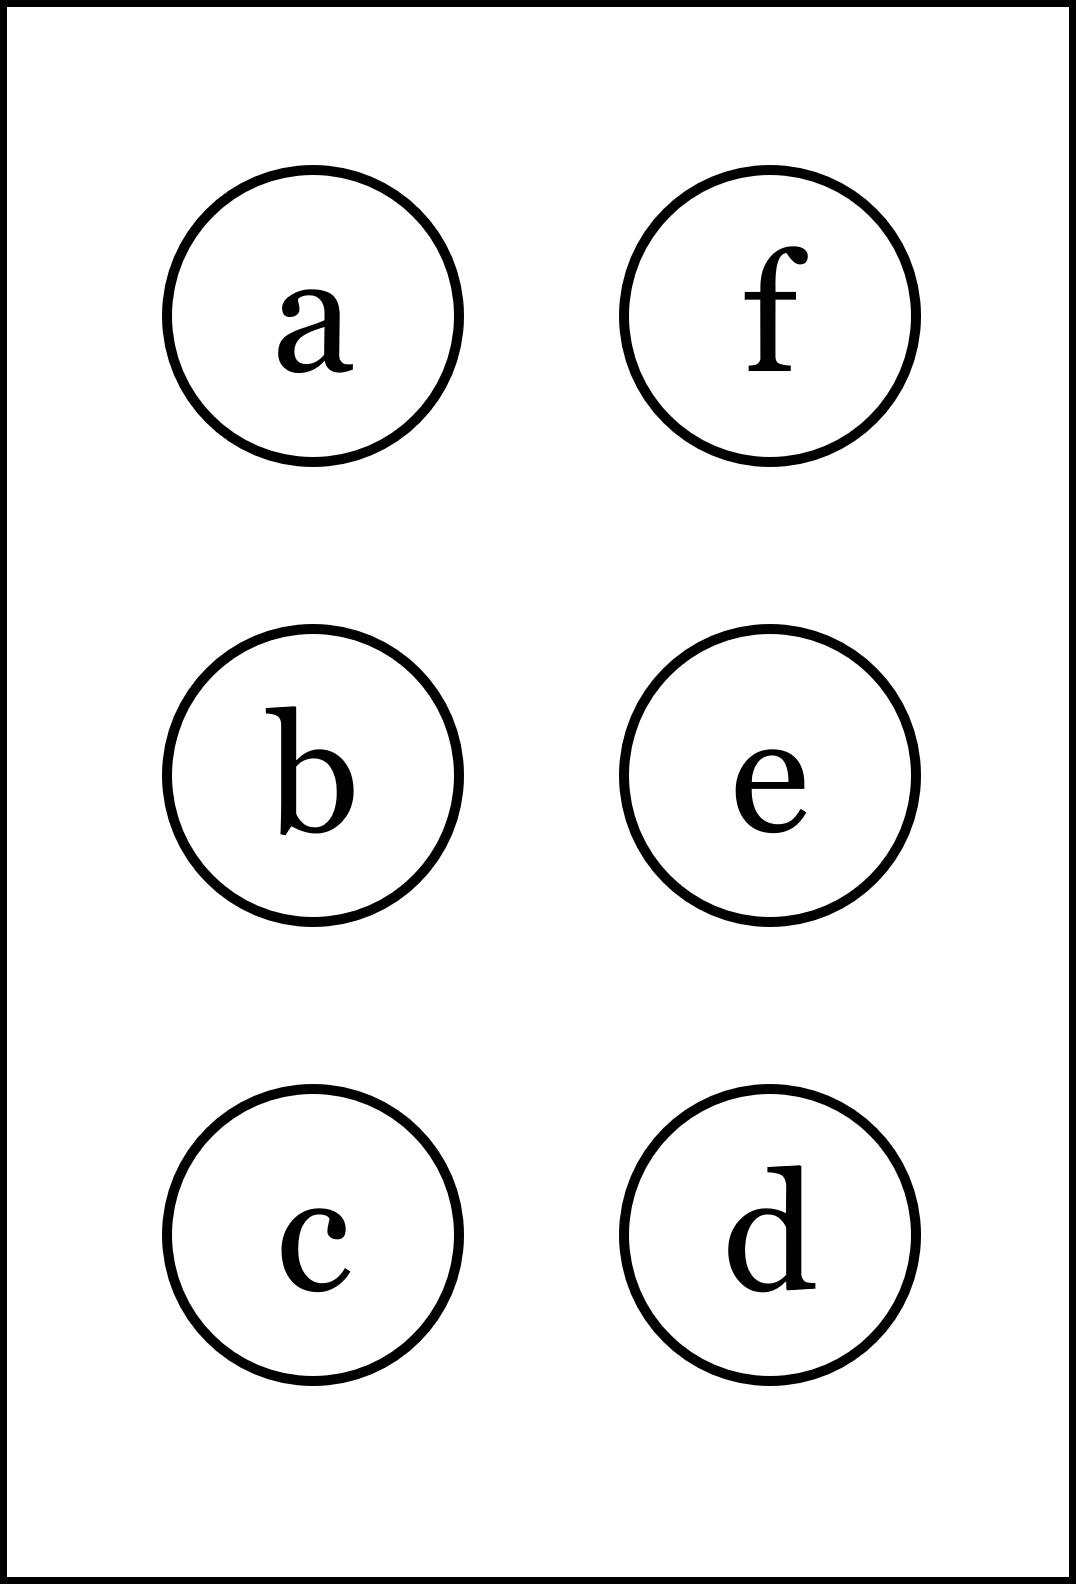
\includegraphics[height=40mm]{../images/braille.png}
{\small Písmeno Braillovej abecedy}
\end{center}
\end{minipage}
\end{center}
\end{minipage}
\\ \hdashline
\begin{minipage}[c][99mm][t]{0.49\linewidth}
\begin{center}
\vspace{7mm}
{\huge Definiční obor, skupina \textit{Mu $\mu$} -\romannumeral3}\\[4.5mm]
\textit{Meno:}\phantom{xxxxxxxxxxxxxxxxxxxxxxxxxxxxxxxxxxxxxxxxxxxxxxxxxxxxxxxxxxxxxxxxx}\\[3.5mm]
\textbf{Zjisti definiční obor} zadaných funkcí. Pokud se shoduje s tím za otazníky,\\tak napravo obarvi příslušející kroužek načerno. \textbf{Spolu odevzdejte výsledné slovo}.\\[3mm]
\begin{minipage}{0.77\linewidth}
\begin{center}
\begin{varwidth}{\textwidth}
\begin{enumerate}
\normalsize
\item $f(x)=\cfrac{-4x+3}{-6x+6}$\quad \dotfill\; ???\;\dotfill \quad $\mathbb{R}\smallsetminus\{1\}$
\item $f(x)=\cfrac{1}{-x^3+3x+2}$\quad \dotfill\; ???\;\dotfill \quad $\mathbb{R}\smallsetminus\{2,-1\}$
\item $f(x)=-2\sqrt{-7x-2}$\quad \dotfill\; ???\;\dotfill \quad $x\leq\nicefrac{-2}{7}$
\item $f(x)=\sqrt{-x^2-7x}$\quad \dotfill\; ???\;\dotfill \quad $x\in(-7 , 0)$
\item $f(x)=-4\ln{(-x+1)}$\quad \dotfill\; ???\;\dotfill \quad $x<-1$
\item $f(x)=\ln{(x^2+12x+27)}$\quad \dotfill\; ???\;\dotfill \quad $x\in(-\infty , -9)\cup(-3 , \infty)$
\end{enumerate}
\end{varwidth}
\end{center}
\end{minipage}
\begin{minipage}{0.20\linewidth}
\begin{center}
{\Huge\bfseries 3.} \\[2mm]
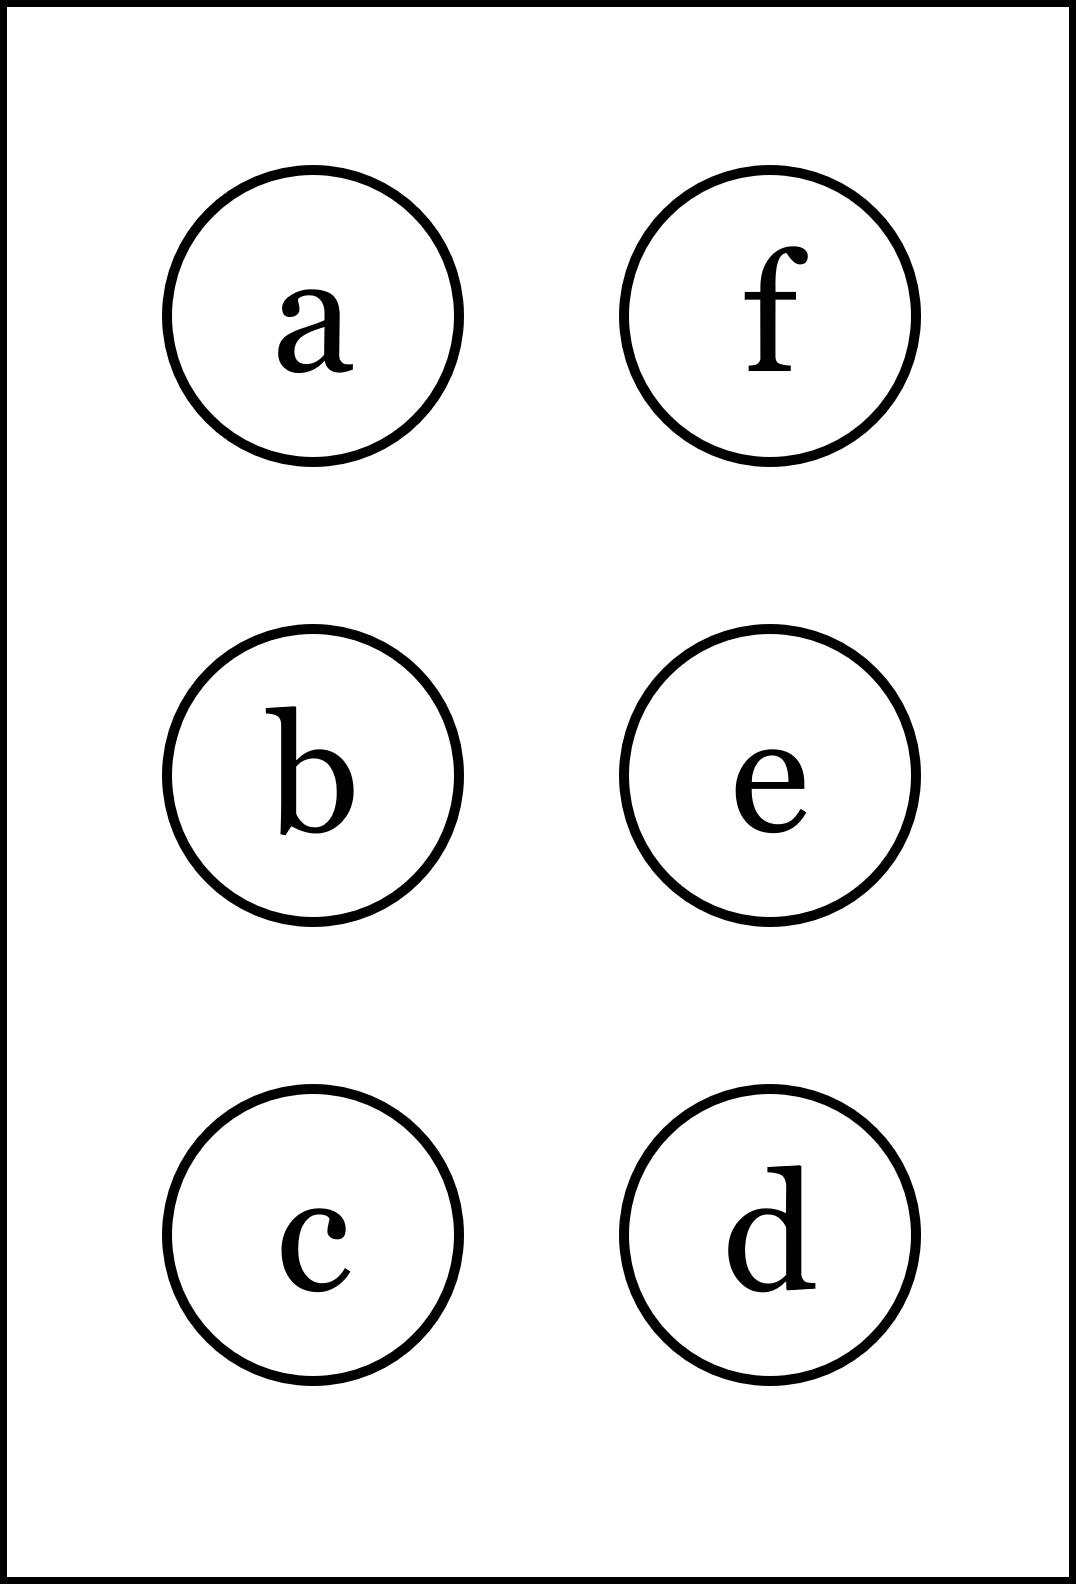
\includegraphics[height=40mm]{../images/braille.png}
{\small Písmeno Braillovej abecedy}
\end{center}
\end{minipage}
\end{center}
\end{minipage}
&
\begin{minipage}[c][99mm][t]{0.49\linewidth}
\begin{center}
\vspace{7mm}
{\huge Definiční obor, skupina \textit{Mu $\mu$} -\romannumeral4}\\[4.5mm]
\textit{Meno:}\phantom{xxxxxxxxxxxxxxxxxxxxxxxxxxxxxxxxxxxxxxxxxxxxxxxxxxxxxxxxxxxxxxxxx}\\[3.5mm]
\textbf{Zjisti definiční obor} zadaných funkcí. Pokud se shoduje s tím za otazníky,\\tak napravo obarvi příslušející kroužek načerno. \textbf{Spolu odevzdejte výsledné slovo}.\\[3mm]
\begin{minipage}{0.77\linewidth}
\begin{center}
\begin{varwidth}{\textwidth}
\begin{enumerate}
\normalsize
\item $f(x)=\cfrac{2x-2}{-8x+6}$\quad \dotfill\; ???\;\dotfill \quad $\mathbb{R}\smallsetminus\{\nicefrac{3}{4}\}$
\item $f(x)=\cfrac{1}{-3x^3-15x^2-21x-9}$\quad \dotfill\; ???\;\dotfill \quad $\mathbb{R}\smallsetminus\{1,-5,-1\}$
\item $f(x)=5\sqrt{-7x-6}$\quad \dotfill\; ???\;\dotfill \quad $x\leq\nicefrac{6}{7}$
\item $f(x)=\sqrt{-x^2-3x}$\quad \dotfill\; ???\;\dotfill \quad $x\in(-3 , 0)$
\item $f(x)=-2\ln{(8x+2)}$\quad \dotfill\; ???\;\dotfill \quad $x>\nicefrac{1}{4}$
\item $f(x)=\ln{(x^2-4)}$\quad \dotfill\; ???\;\dotfill \quad $x\in(-2 , 2)$
\end{enumerate}
\end{varwidth}
\end{center}
\end{minipage}
\begin{minipage}{0.20\linewidth}
\begin{center}
{\Huge\bfseries 4.} \\[2mm]
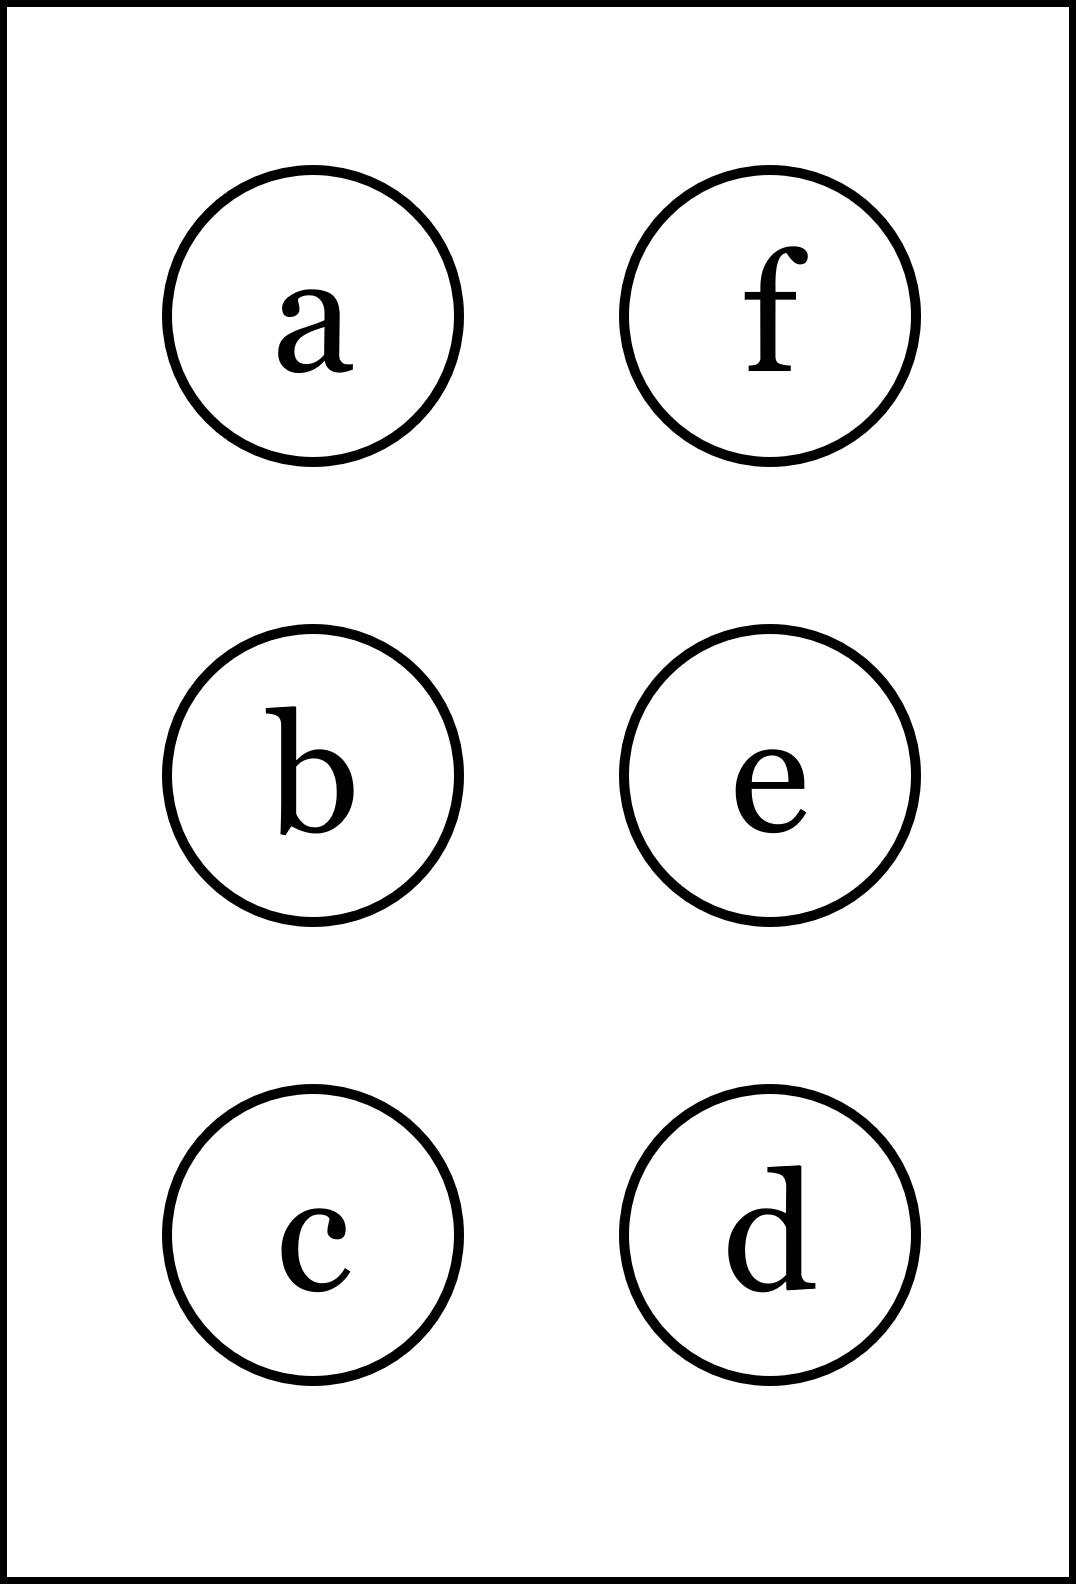
\includegraphics[height=40mm]{../images/braille.png}
{\small Písmeno Braillovej abecedy}
\end{center}
\end{minipage}
\end{center}
\end{minipage}
%
\end{tabular}
\begin{tikzpicture}[remember picture,overlay]\node[xshift=7mm,yshift=-100.6mm,anchor=north west] at (current page.north west){\ding{33}};\end{tikzpicture}
\begin{tikzpicture}[remember picture,overlay]\node[xshift=151.2mm,yshift=-7mm,anchor=north west,rotate=270] at (current page.north west){\ding{33}};\end{tikzpicture}
\newpage
\thispagestyle{empty}
\begin{tabular}{c:c}
\begin{minipage}[c][99mm][t]{0.49\linewidth}
\begin{center}
\vspace{7mm}
{\huge Definiční obor, skupina \textit{Nu $\nu$} -\romannumeral1}\\[4.5mm]
\textit{Meno:}\phantom{xxxxxxxxxxxxxxxxxxxxxxxxxxxxxxxxxxxxxxxxxxxxxxxxxxxxxxxxxxxxxxxxx}\\[3.5mm]
\textbf{Zjisti definiční obor} zadaných funkcí. Pokud se shoduje s tím za otazníky,\\tak napravo obarvi příslušející kroužek načerno. \textbf{Spolu odevzdejte výsledné slovo}.\\[3mm]
\begin{minipage}{0.77\linewidth}
\begin{center}
\begin{varwidth}{\textwidth}
\begin{enumerate}
\normalsize
\item $f(x)=\cfrac{x-4}{2x-6}$\quad \dotfill\; ???\;\dotfill \quad $\mathbb{R}\smallsetminus\{3\}$
\item $f(x)=\cfrac{1}{-x^3-6x^2-11x-6}$\quad \dotfill\; ???\;\dotfill \quad $\mathbb{R}\smallsetminus\{2,-1,-2\}$
\item $f(x)=3\sqrt{2x+6}$\quad \dotfill\; ???\;\dotfill \quad $x\geq-3$
\item $f(x)=\sqrt{-x^2-2x}$\quad \dotfill\; ???\;\dotfill \quad $x\in\langle-2 , 0\rangle$
\item $f(x)=-6\ln{(6x+2)}$\quad \dotfill\; ???\;\dotfill \quad $x<\nicefrac{-1}{3}$
\item $f(x)=\ln{(x^2+3x-18)}$\quad \dotfill\; ???\;\dotfill \quad $x\in(-6 , 3)$
\end{enumerate}
\end{varwidth}
\end{center}
\end{minipage}
\begin{minipage}{0.20\linewidth}
\begin{center}
{\Huge\bfseries 1.} \\[2mm]
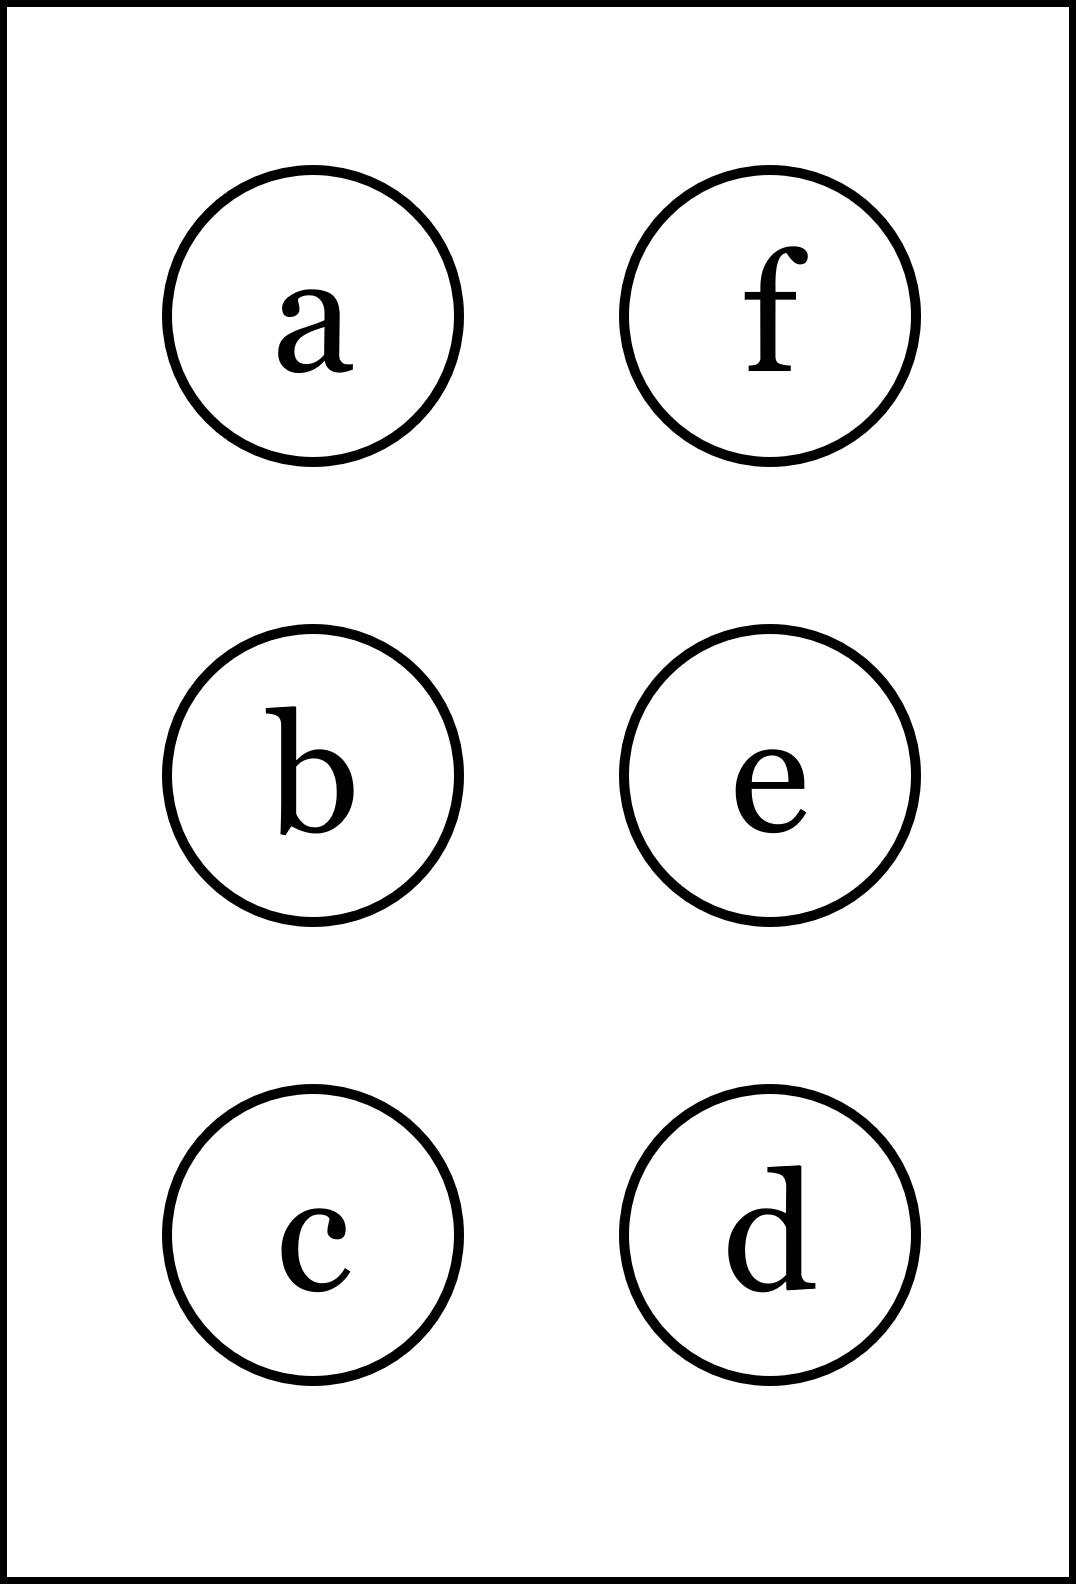
\includegraphics[height=40mm]{../images/braille.png}
{\small Písmeno Braillovej abecedy}
\end{center}
\end{minipage}
\end{center}
\end{minipage}
&
\begin{minipage}[c][99mm][t]{0.49\linewidth}
\begin{center}
\vspace{7mm}
{\huge Definiční obor, skupina \textit{Nu $\nu$} -\romannumeral2}\\[4.5mm]
\textit{Meno:}\phantom{xxxxxxxxxxxxxxxxxxxxxxxxxxxxxxxxxxxxxxxxxxxxxxxxxxxxxxxxxxxxxxxxx}\\[3.5mm]
\textbf{Zjisti definiční obor} zadaných funkcí. Pokud se shoduje s tím za otazníky,\\tak napravo obarvi příslušející kroužek načerno. \textbf{Spolu odevzdejte výsledné slovo}.\\[3mm]
\begin{minipage}{0.77\linewidth}
\begin{center}
\begin{varwidth}{\textwidth}
\begin{enumerate}
\normalsize
\item $f(x)=\cfrac{x-2}{x-2}$\quad \dotfill\; ???\;\dotfill \quad $\mathbb{R}\smallsetminus\{2\}$
\item $f(x)=\cfrac{1}{-x^3+10x^2-23x+14}$\quad \dotfill\; ???\;\dotfill \quad $\mathbb{R}\smallsetminus\{1,2,7\}$
\item $f(x)=-4\sqrt{4x-2}$\quad \dotfill\; ???\;\dotfill \quad $x\geq\nicefrac{1}{2}$
\item $f(x)=\sqrt{-x^2-6x}$\quad \dotfill\; ???\;\dotfill \quad $x\in(-6 , 0)$
\item $f(x)=3\ln{(7x-7)}$\quad \dotfill\; ???\;\dotfill \quad $x>1$
\item $f(x)=\ln{(x^2+3x+2)}$\quad \dotfill\; ???\;\dotfill \quad $x\in(-2 , -1)$
\end{enumerate}
\end{varwidth}
\end{center}
\end{minipage}
\begin{minipage}{0.20\linewidth}
\begin{center}
{\Huge\bfseries 2.} \\[2mm]
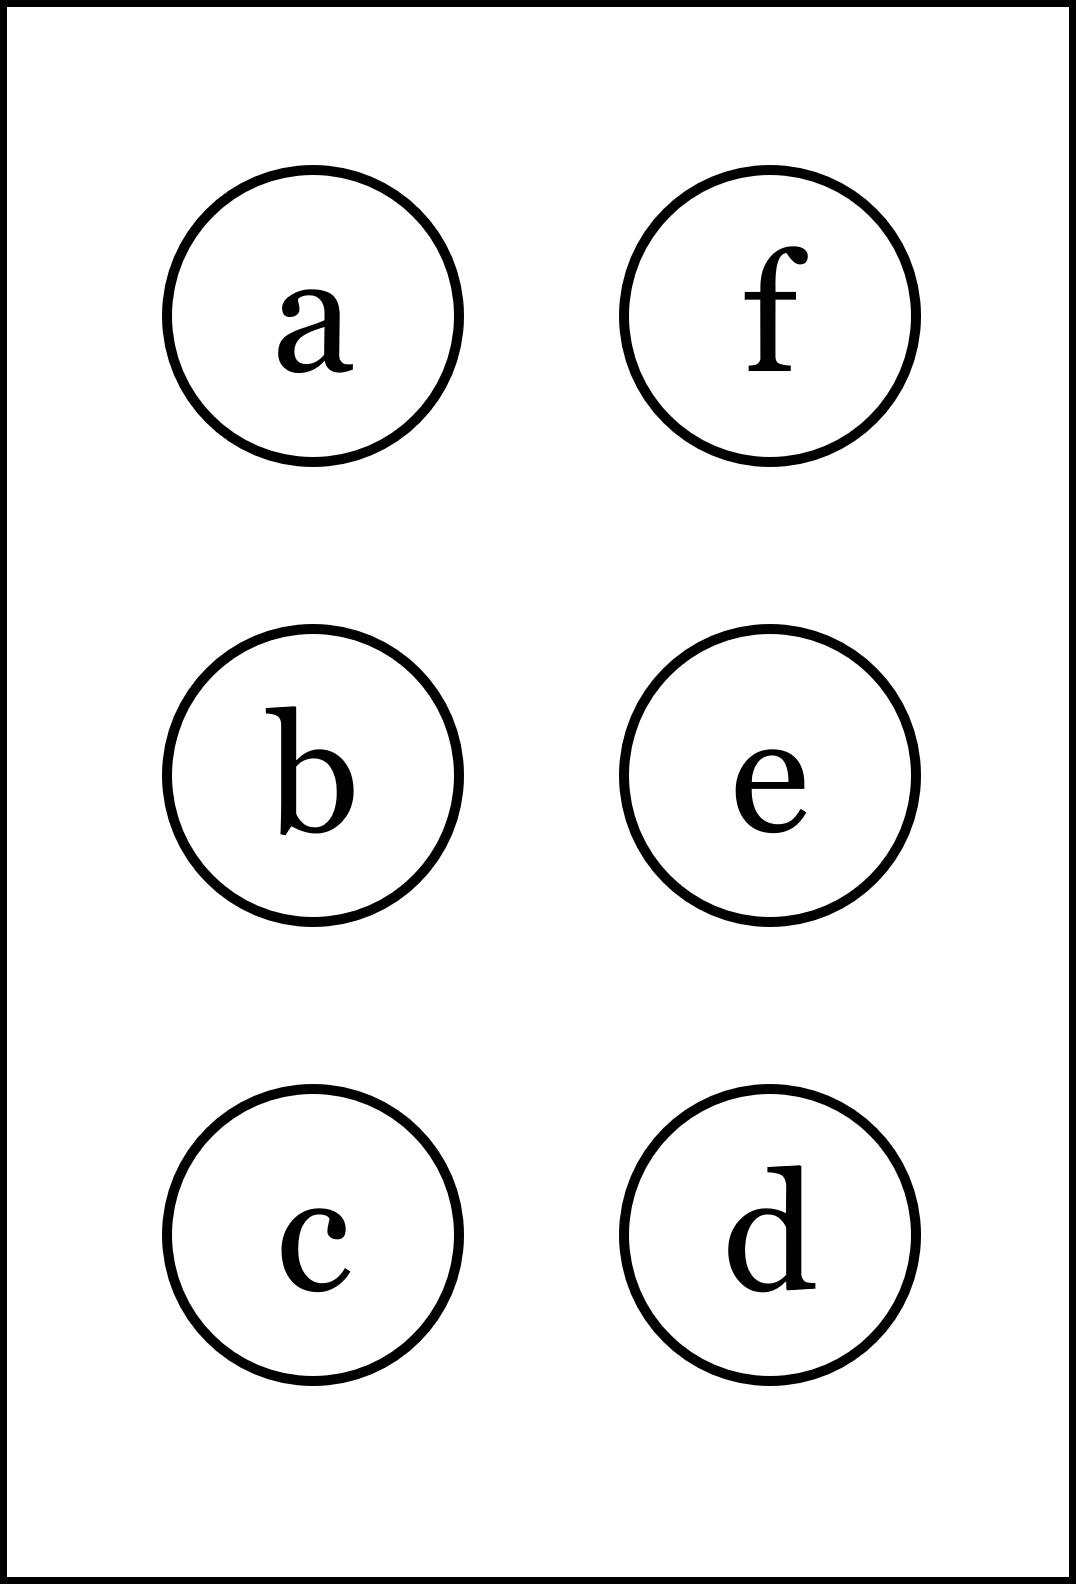
\includegraphics[height=40mm]{../images/braille.png}
{\small Písmeno Braillovej abecedy}
\end{center}
\end{minipage}
\end{center}
\end{minipage}
\\ \hdashline
\begin{minipage}[c][99mm][t]{0.49\linewidth}
\begin{center}
\vspace{7mm}
{\huge Definiční obor, skupina \textit{Nu $\nu$} -\romannumeral3}\\[4.5mm]
\textit{Meno:}\phantom{xxxxxxxxxxxxxxxxxxxxxxxxxxxxxxxxxxxxxxxxxxxxxxxxxxxxxxxxxxxxxxxxx}\\[3.5mm]
\textbf{Zjisti definiční obor} zadaných funkcí. Pokud se shoduje s tím za otazníky,\\tak napravo obarvi příslušející kroužek načerno. \textbf{Spolu odevzdejte výsledné slovo}.\\[3mm]
\begin{minipage}{0.77\linewidth}
\begin{center}
\begin{varwidth}{\textwidth}
\begin{enumerate}
\normalsize
\item $f(x)=\cfrac{2x-3}{-5x+1}$\quad \dotfill\; ???\;\dotfill \quad $\mathbb{R}\smallsetminus\{\nicefrac{1}{5}\}$
\item $f(x)=\cfrac{1}{-2x^3-6x^2+12x+16}$\quad \dotfill\; ???\;\dotfill \quad $\mathbb{R}\smallsetminus\{0,1,-4\}$
\item $f(x)=-7\sqrt{x-4}$\quad \dotfill\; ???\;\dotfill \quad $x\geq4$
\item $f(x)=\sqrt{-x^2+x}$\quad \dotfill\; ???\;\dotfill \quad $x\in(0 , 1)$
\item $f(x)=5\ln{(4x-1)}$\quad \dotfill\; ???\;\dotfill \quad $x>\nicefrac{1}{4}$
\item $f(x)=\ln{(x^2+2x-35)}$\quad \dotfill\; ???\;\dotfill \quad $x\in(-\infty , -7)\cup(5 , \infty)$
\end{enumerate}
\end{varwidth}
\end{center}
\end{minipage}
\begin{minipage}{0.20\linewidth}
\begin{center}
{\Huge\bfseries 3.} \\[2mm]
\includegraphics[height=40mm]{../images/braille.png}
{\small Písmeno Braillovej abecedy}
\end{center}
\end{minipage}
\end{center}
\end{minipage}
&
\begin{minipage}[c][99mm][t]{0.49\linewidth}
\begin{center}
\vspace{7mm}
{\huge Definiční obor, skupina \textit{Nu $\nu$} -\romannumeral4}\\[4.5mm]
\textit{Meno:}\phantom{xxxxxxxxxxxxxxxxxxxxxxxxxxxxxxxxxxxxxxxxxxxxxxxxxxxxxxxxxxxxxxxxx}\\[3.5mm]
\textbf{Zjisti definiční obor} zadaných funkcí. Pokud se shoduje s tím za otazníky,\\tak napravo obarvi příslušející kroužek načerno. \textbf{Spolu odevzdejte výsledné slovo}.\\[3mm]
\begin{minipage}{0.77\linewidth}
\begin{center}
\begin{varwidth}{\textwidth}
\begin{enumerate}
\normalsize
\item $f(x)=\cfrac{2x-5}{5x-3}$\quad \dotfill\; ???\;\dotfill \quad $\mathbb{R}\smallsetminus\{\nicefrac{3}{5}\}$
\item $f(x)=\cfrac{1}{x^3-9x^2+15x-7}$\quad \dotfill\; ???\;\dotfill \quad $\mathbb{R}\smallsetminus\{3,-1,7\}$
\item $f(x)=6\sqrt{4x+3}$\quad \dotfill\; ???\;\dotfill \quad $x\leq\nicefrac{-3}{4}$
\item $f(x)=\sqrt{-x^2+4x}$\quad \dotfill\; ???\;\dotfill \quad $x\in\langle-4 , 0\rangle$
\item $f(x)=-2\ln{(6x-5)}$\quad \dotfill\; ???\;\dotfill \quad $x<\nicefrac{5}{6}$
\item $f(x)=\ln{(x^2-1)}$\quad \dotfill\; ???\;\dotfill \quad $x\in(-1 , 1)$
\end{enumerate}
\end{varwidth}
\end{center}
\end{minipage}
\begin{minipage}{0.20\linewidth}
\begin{center}
{\Huge\bfseries 4.} \\[2mm]
\includegraphics[height=40mm]{../images/braille.png}
{\small Písmeno Braillovej abecedy}
\end{center}
\end{minipage}
\end{center}
\end{minipage}
%
\end{tabular}
\begin{tikzpicture}[remember picture,overlay]\node[xshift=7mm,yshift=-100.6mm,anchor=north west] at (current page.north west){\ding{33}};\end{tikzpicture}
\begin{tikzpicture}[remember picture,overlay]\node[xshift=151.2mm,yshift=-7mm,anchor=north west,rotate=270] at (current page.north west){\ding{33}};\end{tikzpicture}
\newpage
\thispagestyle{empty}
\begin{tabular}{c:c}
\begin{minipage}[c][99mm][t]{0.49\linewidth}
\begin{center}
\vspace{7mm}
{\huge Definiční obor, skupina \textit{Xi $\xi$} -\romannumeral1}\\[4.5mm]
\textit{Meno:}\phantom{xxxxxxxxxxxxxxxxxxxxxxxxxxxxxxxxxxxxxxxxxxxxxxxxxxxxxxxxxxxxxxxxx}\\[3.5mm]
\textbf{Zjisti definiční obor} zadaných funkcí. Pokud se shoduje s tím za otazníky,\\tak napravo obarvi příslušející kroužek načerno. \textbf{Spolu odevzdejte výsledné slovo}.\\[3mm]
\begin{minipage}{0.77\linewidth}
\begin{center}
\begin{varwidth}{\textwidth}
\begin{enumerate}
\normalsize
\item $f(x)=\cfrac{-4x-2}{3x+1}$\quad \dotfill\; ???\;\dotfill \quad $\mathbb{R}\smallsetminus\{\nicefrac{-1}{3}\}$
\item $f(x)=\cfrac{1}{-4x^3+8x^2+20x-24}$\quad \dotfill\; ???\;\dotfill \quad $\mathbb{R}\smallsetminus\{1,2,5\}$
\item $f(x)=-4\sqrt{3x+1}$\quad \dotfill\; ???\;\dotfill \quad $x\leq\nicefrac{-1}{3}$
\item $f(x)=\sqrt{-x^2+4x}$\quad \dotfill\; ???\;\dotfill \quad $x\in(0 , 4)$
\item $f(x)=6\ln{(x-1)}$\quad \dotfill\; ???\;\dotfill \quad $x>-1$
\item $f(x)=\ln{(x^2+8x+12)}$\quad \dotfill\; ???\;\dotfill \quad $x\in(-6 , -2)$
\end{enumerate}
\end{varwidth}
\end{center}
\end{minipage}
\begin{minipage}{0.20\linewidth}
\begin{center}
{\Huge\bfseries 1.} \\[2mm]
\includegraphics[height=40mm]{../images/braille.png}
{\small Písmeno Braillovej abecedy}
\end{center}
\end{minipage}
\end{center}
\end{minipage}
&
\begin{minipage}[c][99mm][t]{0.49\linewidth}
\begin{center}
\vspace{7mm}
{\huge Definiční obor, skupina \textit{Xi $\xi$} -\romannumeral2}\\[4.5mm]
\textit{Meno:}\phantom{xxxxxxxxxxxxxxxxxxxxxxxxxxxxxxxxxxxxxxxxxxxxxxxxxxxxxxxxxxxxxxxxx}\\[3.5mm]
\textbf{Zjisti definiční obor} zadaných funkcí. Pokud se shoduje s tím za otazníky,\\tak napravo obarvi příslušející kroužek načerno. \textbf{Spolu odevzdejte výsledné slovo}.\\[3mm]
\begin{minipage}{0.77\linewidth}
\begin{center}
\begin{varwidth}{\textwidth}
\begin{enumerate}
\normalsize
\item $f(x)=\cfrac{-x+3}{-8x-5}$\quad \dotfill\; ???\;\dotfill \quad $\mathbb{R}\smallsetminus\{\nicefrac{-5}{8}\}$
\item $f(x)=\cfrac{1}{-x^3+9x^2+x-9}$\quad \dotfill\; ???\;\dotfill \quad $\mathbb{R}\smallsetminus\{0,-1,-9\}$
\item $f(x)=3\sqrt{-7x-7}$\quad \dotfill\; ???\;\dotfill \quad $x\leq-1$
\item $f(x)=\sqrt{-x^2-6x}$\quad \dotfill\; ???\;\dotfill \quad $x\in(-6 , 0)$
\item $f(x)=-5\ln{(-2x-4)}$\quad \dotfill\; ???\;\dotfill \quad $x<-2$
\item $f(x)=\ln{(x^2-x-6)}$\quad \dotfill\; ???\;\dotfill \quad $x\in(-\infty , -2)\cup(3 , \infty)$
\end{enumerate}
\end{varwidth}
\end{center}
\end{minipage}
\begin{minipage}{0.20\linewidth}
\begin{center}
{\Huge\bfseries 2.} \\[2mm]
\includegraphics[height=40mm]{../images/braille.png}
{\small Písmeno Braillovej abecedy}
\end{center}
\end{minipage}
\end{center}
\end{minipage}
\\ \hdashline
\begin{minipage}[c][99mm][t]{0.49\linewidth}
\begin{center}
\vspace{7mm}
{\huge Definiční obor, skupina \textit{Xi $\xi$} -\romannumeral3}\\[4.5mm]
\textit{Meno:}\phantom{xxxxxxxxxxxxxxxxxxxxxxxxxxxxxxxxxxxxxxxxxxxxxxxxxxxxxxxxxxxxxxxxx}\\[3.5mm]
\textbf{Zjisti definiční obor} zadaných funkcí. Pokud se shoduje s tím za otazníky,\\tak napravo obarvi příslušející kroužek načerno. \textbf{Spolu odevzdejte výsledné slovo}.\\[3mm]
\begin{minipage}{0.77\linewidth}
\begin{center}
\begin{varwidth}{\textwidth}
\begin{enumerate}
\normalsize
\item $f(x)=\cfrac{-4x+1}{x+3}$\quad \dotfill\; ???\;\dotfill \quad $\mathbb{R}\smallsetminus\{-3\}$
\item $f(x)=\cfrac{1}{-6x^3+30x^2-48x+24}$\quad \dotfill\; ???\;\dotfill \quad $\mathbb{R}\smallsetminus\{2,-2\}$
\item $f(x)=-8\sqrt{-6x+2}$\quad \dotfill\; ???\;\dotfill \quad $x\leq\nicefrac{1}{3}$
\item $f(x)=\sqrt{-x^2+7x}$\quad \dotfill\; ???\;\dotfill \quad $x\in\langle-7 , 0\rangle$
\item $f(x)=7\ln{(6x-2)}$\quad \dotfill\; ???\;\dotfill \quad $x>\nicefrac{1}{3}$
\item $f(x)=\ln{(x^2-3x-28)}$\quad \dotfill\; ???\;\dotfill \quad $x\in(-\infty , -4)\cup(7 , \infty)$
\end{enumerate}
\end{varwidth}
\end{center}
\end{minipage}
\begin{minipage}{0.20\linewidth}
\begin{center}
{\Huge\bfseries 3.} \\[2mm]
\includegraphics[height=40mm]{../images/braille.png}
{\small Písmeno Braillovej abecedy}
\end{center}
\end{minipage}
\end{center}
\end{minipage}
&
\begin{minipage}[c][99mm][t]{0.49\linewidth}
\begin{center}
\vspace{7mm}
{\huge Definiční obor, skupina \textit{Xi $\xi$} -\romannumeral4}\\[4.5mm]
\textit{Meno:}\phantom{xxxxxxxxxxxxxxxxxxxxxxxxxxxxxxxxxxxxxxxxxxxxxxxxxxxxxxxxxxxxxxxxx}\\[3.5mm]
\textbf{Zjisti definiční obor} zadaných funkcí. Pokud se shoduje s tím za otazníky,\\tak napravo obarvi příslušející kroužek načerno. \textbf{Spolu odevzdejte výsledné slovo}.\\[3mm]
\begin{minipage}{0.77\linewidth}
\begin{center}
\begin{varwidth}{\textwidth}
\begin{enumerate}
\normalsize
\item $f(x)=\cfrac{4x+1}{9x+8}$\quad \dotfill\; ???\;\dotfill \quad $\mathbb{R}\smallsetminus\{\nicefrac{-8}{9}\}$
\item $f(x)=\cfrac{1}{-2x^3-6x^2+8x+24}$\quad \dotfill\; ???\;\dotfill \quad $\mathbb{R}\smallsetminus\{2,-4\}$
\item $f(x)=1\sqrt{2x+7}$\quad \dotfill\; ???\;\dotfill \quad $x\leq\nicefrac{-7}{2}$
\item $f(x)=\sqrt{-x^2+x}$\quad \dotfill\; ???\;\dotfill \quad $x\in(0 , 1)$
\item $f(x)=-7\ln{(x+3)}$\quad \dotfill\; ???\;\dotfill \quad $x>3$
\item $f(x)=\ln{(x^2-2x+1)}$\quad \dotfill\; ???\;\dotfill \quad $x\in(1 , 1)$
\end{enumerate}
\end{varwidth}
\end{center}
\end{minipage}
\begin{minipage}{0.20\linewidth}
\begin{center}
{\Huge\bfseries 4.} \\[2mm]
\includegraphics[height=40mm]{../images/braille.png}
{\small Písmeno Braillovej abecedy}
\end{center}
\end{minipage}
\end{center}
\end{minipage}
%
\end{tabular}
\begin{tikzpicture}[remember picture,overlay]\node[xshift=7mm,yshift=-100.6mm,anchor=north west] at (current page.north west){\ding{33}};\end{tikzpicture}
\begin{tikzpicture}[remember picture,overlay]\node[xshift=151.2mm,yshift=-7mm,anchor=north west,rotate=270] at (current page.north west){\ding{33}};\end{tikzpicture}
\newpage
\thispagestyle{empty}
\begin{tabular}{c:c}
\begin{minipage}[c][99mm][t]{0.49\linewidth}
\begin{center}
\vspace{7mm}
{\huge Definiční obor, skupina \textit{Omicron $\omicron$} -\romannumeral1}\\[4.5mm]
\textit{Meno:}\phantom{xxxxxxxxxxxxxxxxxxxxxxxxxxxxxxxxxxxxxxxxxxxxxxxxxxxxxxxxxxxxxxxxx}\\[3.5mm]
\textbf{Zjisti definiční obor} zadaných funkcí. Pokud se shoduje s tím za otazníky,\\tak napravo obarvi příslušející kroužek načerno. \textbf{Spolu odevzdejte výsledné slovo}.\\[3mm]
\begin{minipage}{0.77\linewidth}
\begin{center}
\begin{varwidth}{\textwidth}
\begin{enumerate}
\normalsize
\item $f(x)=\cfrac{-3x+2}{2x+3}$\quad \dotfill\; ???\;\dotfill \quad $\mathbb{R}\smallsetminus\{\nicefrac{-3}{2}\}$
\item $f(x)=\cfrac{1}{3x^3+18x^2+33x+18}$\quad \dotfill\; ???\;\dotfill \quad $\mathbb{R}\smallsetminus\{-3,-1,-2\}$
\item $f(x)=-9\sqrt{9x-1}$\quad \dotfill\; ???\;\dotfill \quad $x\geq\nicefrac{1}{9}$
\item $f(x)=\sqrt{-x^2-2x}$\quad \dotfill\; ???\;\dotfill \quad $x\in(-2 , 0)$
\item $f(x)=2\ln{(x-8)}$\quad \dotfill\; ???\;\dotfill \quad $x<8$
\item $f(x)=\ln{(x^2-25)}$\quad \dotfill\; ???\;\dotfill \quad $x\in(-\infty , -5)\cup(5 , \infty)$
\end{enumerate}
\end{varwidth}
\end{center}
\end{minipage}
\begin{minipage}{0.20\linewidth}
\begin{center}
{\Huge\bfseries 1.} \\[2mm]
\includegraphics[height=40mm]{../images/braille.png}
{\small Písmeno Braillovej abecedy}
\end{center}
\end{minipage}
\end{center}
\end{minipage}
&
\begin{minipage}[c][99mm][t]{0.49\linewidth}
\begin{center}
\vspace{7mm}
{\huge Definiční obor, skupina \textit{Omicron $\omicron$} -\romannumeral2}\\[4.5mm]
\textit{Meno:}\phantom{xxxxxxxxxxxxxxxxxxxxxxxxxxxxxxxxxxxxxxxxxxxxxxxxxxxxxxxxxxxxxxxxx}\\[3.5mm]
\textbf{Zjisti definiční obor} zadaných funkcí. Pokud se shoduje s tím za otazníky,\\tak napravo obarvi příslušející kroužek načerno. \textbf{Spolu odevzdejte výsledné slovo}.\\[3mm]
\begin{minipage}{0.77\linewidth}
\begin{center}
\begin{varwidth}{\textwidth}
\begin{enumerate}
\normalsize
\item $f(x)=\cfrac{5x+1}{-x+4}$\quad \dotfill\; ???\;\dotfill \quad $\mathbb{R}\smallsetminus\{-4\}$
\item $f(x)=\cfrac{1}{2x^3-4x^2-2x+4}$\quad \dotfill\; ???\;\dotfill \quad $\mathbb{R}\smallsetminus\{1,2,-1\}$
\item $f(x)=1\sqrt{-2x+2}$\quad \dotfill\; ???\;\dotfill \quad $x\leq-1$
\item $f(x)=\sqrt{-x^2-x}$\quad \dotfill\; ???\;\dotfill \quad $x\in\langle0 , 1\rangle$
\item $f(x)=1\ln{(-5x+1)}$\quad \dotfill\; ???\;\dotfill \quad $x<\nicefrac{-1}{5}$
\item $f(x)=\ln{(x^2+5x-6)}$\quad \dotfill\; ???\;\dotfill \quad $x\in(-\infty , -6)\cup(1 , \infty)$
\end{enumerate}
\end{varwidth}
\end{center}
\end{minipage}
\begin{minipage}{0.20\linewidth}
\begin{center}
{\Huge\bfseries 2.} \\[2mm]
\includegraphics[height=40mm]{../images/braille.png}
{\small Písmeno Braillovej abecedy}
\end{center}
\end{minipage}
\end{center}
\end{minipage}
\\ \hdashline
\begin{minipage}[c][99mm][t]{0.49\linewidth}
\begin{center}
\vspace{7mm}
{\huge Definiční obor, skupina \textit{Omicron $\omicron$} -\romannumeral3}\\[4.5mm]
\textit{Meno:}\phantom{xxxxxxxxxxxxxxxxxxxxxxxxxxxxxxxxxxxxxxxxxxxxxxxxxxxxxxxxxxxxxxxxx}\\[3.5mm]
\textbf{Zjisti definiční obor} zadaných funkcí. Pokud se shoduje s tím za otazníky,\\tak napravo obarvi příslušející kroužek načerno. \textbf{Spolu odevzdejte výsledné slovo}.\\[3mm]
\begin{minipage}{0.77\linewidth}
\begin{center}
\begin{varwidth}{\textwidth}
\begin{enumerate}
\normalsize
\item $f(x)=\cfrac{-3x+4}{-5x+2}$\quad \dotfill\; ???\;\dotfill \quad $\mathbb{R}\smallsetminus\{\nicefrac{2}{5}\}$
\item $f(x)=\cfrac{1}{2x^3+8x^2+10x+4}$\quad \dotfill\; ???\;\dotfill \quad $\mathbb{R}\smallsetminus\{-1,-2\}$
\item $f(x)=1\sqrt{2x-8}$\quad \dotfill\; ???\;\dotfill \quad $x\geq4$
\item $f(x)=\sqrt{-x^2+x}$\quad \dotfill\; ???\;\dotfill \quad $x\in\langle0 , 1\rangle$
\item $f(x)=5\ln{(x-5)}$\quad \dotfill\; ???\;\dotfill \quad $x<5$
\item $f(x)=\ln{(x^2-4)}$\quad \dotfill\; ???\;\dotfill \quad $x\in(-2 , 2)$
\end{enumerate}
\end{varwidth}
\end{center}
\end{minipage}
\begin{minipage}{0.20\linewidth}
\begin{center}
{\Huge\bfseries 3.} \\[2mm]
\includegraphics[height=40mm]{../images/braille.png}
{\small Písmeno Braillovej abecedy}
\end{center}
\end{minipage}
\end{center}
\end{minipage}
&
\begin{minipage}[c][99mm][t]{0.49\linewidth}
\begin{center}
\vspace{7mm}
{\huge Definiční obor, skupina \textit{Omicron $\omicron$} -\romannumeral4}\\[4.5mm]
\textit{Meno:}\phantom{xxxxxxxxxxxxxxxxxxxxxxxxxxxxxxxxxxxxxxxxxxxxxxxxxxxxxxxxxxxxxxxxx}\\[3.5mm]
\textbf{Zjisti definiční obor} zadaných funkcí. Pokud se shoduje s tím za otazníky,\\tak napravo obarvi příslušející kroužek načerno. \textbf{Spolu odevzdejte výsledné slovo}.\\[3mm]
\begin{minipage}{0.77\linewidth}
\begin{center}
\begin{varwidth}{\textwidth}
\begin{enumerate}
\normalsize
\item $f(x)=\cfrac{x+8}{-4x+3}$\quad \dotfill\; ???\;\dotfill \quad $\mathbb{R}\smallsetminus\{\nicefrac{3}{4}\}$
\item $f(x)=\cfrac{1}{-2x^3+4x^2+10x-12}$\quad \dotfill\; ???\;\dotfill \quad $\mathbb{R}\smallsetminus\{1,-4,-3\}$
\item $f(x)=5\sqrt{2x-3}$\quad \dotfill\; ???\;\dotfill \quad $x\geq\nicefrac{3}{2}$
\item $f(x)=\sqrt{-x^2-7x}$\quad \dotfill\; ???\;\dotfill \quad $x\in\langle0 , 7\rangle$
\item $f(x)=2\ln{(5x+3)}$\quad \dotfill\; ???\;\dotfill \quad $x>\nicefrac{-3}{5}$
\item $f(x)=\ln{(x^2-9)}$\quad \dotfill\; ???\;\dotfill \quad $x\in(-3 , 3)$
\end{enumerate}
\end{varwidth}
\end{center}
\end{minipage}
\begin{minipage}{0.20\linewidth}
\begin{center}
{\Huge\bfseries 4.} \\[2mm]
\includegraphics[height=40mm]{../images/braille.png}
{\small Písmeno Braillovej abecedy}
\end{center}
\end{minipage}
\end{center}
\end{minipage}
%
\end{tabular}
\begin{tikzpicture}[remember picture,overlay]\node[xshift=7mm,yshift=-100.6mm,anchor=north west] at (current page.north west){\ding{33}};\end{tikzpicture}
\begin{tikzpicture}[remember picture,overlay]\node[xshift=151.2mm,yshift=-7mm,anchor=north west,rotate=270] at (current page.north west){\ding{33}};\end{tikzpicture}
\newpage
\thispagestyle{empty}
\begin{tabular}{c:c}
\begin{minipage}[c][99mm][t]{0.49\linewidth}
\begin{center}
\vspace{7mm}
{\huge Definiční obor, skupina \textit{Pi $\pi$} -\romannumeral1}\\[4.5mm]
\textit{Meno:}\phantom{xxxxxxxxxxxxxxxxxxxxxxxxxxxxxxxxxxxxxxxxxxxxxxxxxxxxxxxxxxxxxxxxx}\\[3.5mm]
\textbf{Zjisti definiční obor} zadaných funkcí. Pokud se shoduje s tím za otazníky,\\tak napravo obarvi příslušející kroužek načerno. \textbf{Spolu odevzdejte výsledné slovo}.\\[3mm]
\begin{minipage}{0.77\linewidth}
\begin{center}
\begin{varwidth}{\textwidth}
\begin{enumerate}
\normalsize
\item $f(x)=\cfrac{3x-6}{x-3}$\quad \dotfill\; ???\;\dotfill \quad $\mathbb{R}\smallsetminus\{3\}$
\item $f(x)=\cfrac{1}{x^3+7x^2-4x-28}$\quad \dotfill\; ???\;\dotfill \quad $\mathbb{R}\smallsetminus\{-5,-2\}$
\item $f(x)=-5\sqrt{-5x+5}$\quad \dotfill\; ???\;\dotfill \quad $x\geq1$
\item $f(x)=\sqrt{-x^2+8x}$\quad \dotfill\; ???\;\dotfill \quad $x\in\langle0 , 8\rangle$
\item $f(x)=9\ln{(-3x-2)}$\quad \dotfill\; ???\;\dotfill \quad $x<\nicefrac{-2}{3}$
\item $f(x)=\ln{(x^2+7x+12)}$\quad \dotfill\; ???\;\dotfill \quad $x\in(-4 , -3)$
\end{enumerate}
\end{varwidth}
\end{center}
\end{minipage}
\begin{minipage}{0.20\linewidth}
\begin{center}
{\Huge\bfseries 1.} \\[2mm]
\includegraphics[height=40mm]{../images/braille.png}
{\small Písmeno Braillovej abecedy}
\end{center}
\end{minipage}
\end{center}
\end{minipage}
&
\begin{minipage}[c][99mm][t]{0.49\linewidth}
\begin{center}
\vspace{7mm}
{\huge Definiční obor, skupina \textit{Pi $\pi$} -\romannumeral2}\\[4.5mm]
\textit{Meno:}\phantom{xxxxxxxxxxxxxxxxxxxxxxxxxxxxxxxxxxxxxxxxxxxxxxxxxxxxxxxxxxxxxxxxx}\\[3.5mm]
\textbf{Zjisti definiční obor} zadaných funkcí. Pokud se shoduje s tím za otazníky,\\tak napravo obarvi příslušející kroužek načerno. \textbf{Spolu odevzdejte výsledné slovo}.\\[3mm]
\begin{minipage}{0.77\linewidth}
\begin{center}
\begin{varwidth}{\textwidth}
\begin{enumerate}
\normalsize
\item $f(x)=\cfrac{-2x-3}{6x-3}$\quad \dotfill\; ???\;\dotfill \quad $\mathbb{R}\smallsetminus\{\nicefrac{1}{2}\}$
\item $f(x)=\cfrac{1}{-4x^3+20x^2-28x+12}$\quad \dotfill\; ???\;\dotfill \quad $\mathbb{R}\smallsetminus\{1,5,-1\}$
\item $f(x)=-3\sqrt{-2x+4}$\quad \dotfill\; ???\;\dotfill \quad $x\leq2$
\item $f(x)=\sqrt{-x^2+8x}$\quad \dotfill\; ???\;\dotfill \quad $x\in(0 , 8)$
\item $f(x)=9\ln{(-x+7)}$\quad \dotfill\; ???\;\dotfill \quad $x<7$
\item $f(x)=\ln{(x^2-6x+8)}$\quad \dotfill\; ???\;\dotfill \quad $x\in(-\infty , 2)\cup(4 , \infty)$
\end{enumerate}
\end{varwidth}
\end{center}
\end{minipage}
\begin{minipage}{0.20\linewidth}
\begin{center}
{\Huge\bfseries 2.} \\[2mm]
\includegraphics[height=40mm]{../images/braille.png}
{\small Písmeno Braillovej abecedy}
\end{center}
\end{minipage}
\end{center}
\end{minipage}
\\ \hdashline
\begin{minipage}[c][99mm][t]{0.49\linewidth}
\begin{center}
\vspace{7mm}
{\huge Definiční obor, skupina \textit{Pi $\pi$} -\romannumeral3}\\[4.5mm]
\textit{Meno:}\phantom{xxxxxxxxxxxxxxxxxxxxxxxxxxxxxxxxxxxxxxxxxxxxxxxxxxxxxxxxxxxxxxxxx}\\[3.5mm]
\textbf{Zjisti definiční obor} zadaných funkcí. Pokud se shoduje s tím za otazníky,\\tak napravo obarvi příslušející kroužek načerno. \textbf{Spolu odevzdejte výsledné slovo}.\\[3mm]
\begin{minipage}{0.77\linewidth}
\begin{center}
\begin{varwidth}{\textwidth}
\begin{enumerate}
\normalsize
\item $f(x)=\cfrac{-x-3}{2x+1}$\quad \dotfill\; ???\;\dotfill \quad $\mathbb{R}\smallsetminus\{\nicefrac{-1}{2}\}$
\item $f(x)=\cfrac{1}{7x^3-35x^2+14x+56}$\quad \dotfill\; ???\;\dotfill \quad $\mathbb{R}\smallsetminus\{1,2,5\}$
\item $f(x)=-5\sqrt{3x+7}$\quad \dotfill\; ???\;\dotfill \quad $x\geq\nicefrac{7}{3}$
\item $f(x)=\sqrt{-x^2+x}$\quad \dotfill\; ???\;\dotfill \quad $x\in(0 , 1)$
\item $f(x)=-3\ln{(x+3)}$\quad \dotfill\; ???\;\dotfill \quad $x>-3$
\item $f(x)=\ln{(x^2-2x-3)}$\quad \dotfill\; ???\;\dotfill \quad $x\in(-1 , 3)$
\end{enumerate}
\end{varwidth}
\end{center}
\end{minipage}
\begin{minipage}{0.20\linewidth}
\begin{center}
{\Huge\bfseries 3.} \\[2mm]
\includegraphics[height=40mm]{../images/braille.png}
{\small Písmeno Braillovej abecedy}
\end{center}
\end{minipage}
\end{center}
\end{minipage}
&
\begin{minipage}[c][99mm][t]{0.49\linewidth}
\begin{center}
\vspace{7mm}
{\huge Definiční obor, skupina \textit{Pi $\pi$} -\romannumeral4}\\[4.5mm]
\textit{Meno:}\phantom{xxxxxxxxxxxxxxxxxxxxxxxxxxxxxxxxxxxxxxxxxxxxxxxxxxxxxxxxxxxxxxxxx}\\[3.5mm]
\textbf{Zjisti definiční obor} zadaných funkcí. Pokud se shoduje s tím za otazníky,\\tak napravo obarvi příslušející kroužek načerno. \textbf{Spolu odevzdejte výsledné slovo}.\\[3mm]
\begin{minipage}{0.77\linewidth}
\begin{center}
\begin{varwidth}{\textwidth}
\begin{enumerate}
\normalsize
\item $f(x)=\cfrac{-x+5}{2x-5}$\quad \dotfill\; ???\;\dotfill \quad $\mathbb{R}\smallsetminus\{\nicefrac{5}{2}\}$
\item $f(x)=\cfrac{1}{-4x^3+28x+24}$\quad \dotfill\; ???\;\dotfill \quad $\mathbb{R}\smallsetminus\{0,1,3\}$
\item $f(x)=3\sqrt{-5x-3}$\quad \dotfill\; ???\;\dotfill \quad $x\leq\nicefrac{-3}{5}$
\item $f(x)=\sqrt{-x^2+4x}$\quad \dotfill\; ???\;\dotfill \quad $x\in(0 , 4)$
\item $f(x)=1\ln{(5x-5)}$\quad \dotfill\; ???\;\dotfill \quad $x<1$
\item $f(x)=\ln{(x^2+5x+6)}$\quad \dotfill\; ???\;\dotfill \quad $x\in(-3 , -2)$
\end{enumerate}
\end{varwidth}
\end{center}
\end{minipage}
\begin{minipage}{0.20\linewidth}
\begin{center}
{\Huge\bfseries 4.} \\[2mm]
\includegraphics[height=40mm]{../images/braille.png}
{\small Písmeno Braillovej abecedy}
\end{center}
\end{minipage}
\end{center}
\end{minipage}
%
\end{tabular}
\begin{tikzpicture}[remember picture,overlay]\node[xshift=7mm,yshift=-100.6mm,anchor=north west] at (current page.north west){\ding{33}};\end{tikzpicture}
\begin{tikzpicture}[remember picture,overlay]\node[xshift=151.2mm,yshift=-7mm,anchor=north west,rotate=270] at (current page.north west){\ding{33}};\end{tikzpicture}
\newpage
\thispagestyle{empty}
\begin{tabular}{c:c}
\begin{minipage}[c][99mm][t]{0.49\linewidth}
\begin{center}
\vspace{7mm}
{\huge Definiční obor, skupina \textit{Rho $\rho$} -\romannumeral1}\\[4.5mm]
\textit{Meno:}\phantom{xxxxxxxxxxxxxxxxxxxxxxxxxxxxxxxxxxxxxxxxxxxxxxxxxxxxxxxxxxxxxxxxx}\\[3.5mm]
\textbf{Zjisti definiční obor} zadaných funkcí. Pokud se shoduje s tím za otazníky,\\tak napravo obarvi příslušející kroužek načerno. \textbf{Spolu odevzdejte výsledné slovo}.\\[3mm]
\begin{minipage}{0.77\linewidth}
\begin{center}
\begin{varwidth}{\textwidth}
\begin{enumerate}
\normalsize
\item $f(x)=\cfrac{9x-4}{x-7}$\quad \dotfill\; ???\;\dotfill \quad $\mathbb{R}\smallsetminus\{7\}$
\item $f(x)=\cfrac{1}{x^3-13x^2+50x-56}$\quad \dotfill\; ???\;\dotfill \quad $\mathbb{R}\smallsetminus\{2,4,7\}$
\item $f(x)=3\sqrt{-6x-8}$\quad \dotfill\; ???\;\dotfill \quad $x\leq\nicefrac{4}{3}$
\item $f(x)=\sqrt{-x^2+2x}$\quad \dotfill\; ???\;\dotfill \quad $x\in\langle-2 , 0\rangle$
\item $f(x)=1\ln{(2x+6)}$\quad \dotfill\; ???\;\dotfill \quad $x>3$
\item $f(x)=\ln{(x^2-3x-4)}$\quad \dotfill\; ???\;\dotfill \quad $x\in(-1 , 4)$
\end{enumerate}
\end{varwidth}
\end{center}
\end{minipage}
\begin{minipage}{0.20\linewidth}
\begin{center}
{\Huge\bfseries 1.} \\[2mm]
\includegraphics[height=40mm]{../images/braille.png}
{\small Písmeno Braillovej abecedy}
\end{center}
\end{minipage}
\end{center}
\end{minipage}
&
\begin{minipage}[c][99mm][t]{0.49\linewidth}
\begin{center}
\vspace{7mm}
{\huge Definiční obor, skupina \textit{Rho $\rho$} -\romannumeral2}\\[4.5mm]
\textit{Meno:}\phantom{xxxxxxxxxxxxxxxxxxxxxxxxxxxxxxxxxxxxxxxxxxxxxxxxxxxxxxxxxxxxxxxxx}\\[3.5mm]
\textbf{Zjisti definiční obor} zadaných funkcí. Pokud se shoduje s tím za otazníky,\\tak napravo obarvi příslušející kroužek načerno. \textbf{Spolu odevzdejte výsledné slovo}.\\[3mm]
\begin{minipage}{0.77\linewidth}
\begin{center}
\begin{varwidth}{\textwidth}
\begin{enumerate}
\normalsize
\item $f(x)=\cfrac{7x-3}{-7x+3}$\quad \dotfill\; ???\;\dotfill \quad $\mathbb{R}\smallsetminus\{\nicefrac{3}{7}\}$
\item $f(x)=\cfrac{1}{-x^3-14x^2-51x-54}$\quad \dotfill\; ???\;\dotfill \quad $\mathbb{R}\smallsetminus\{2,-3,-10\}$
\item $f(x)=-1\sqrt{-5x-2}$\quad \dotfill\; ???\;\dotfill \quad $x\leq\nicefrac{-2}{5}$
\item $f(x)=\sqrt{-x^2+7x}$\quad \dotfill\; ???\;\dotfill \quad $x\in\langle-7 , 0\rangle$
\item $f(x)=2\ln{(6x-8)}$\quad \dotfill\; ???\;\dotfill \quad $x>\nicefrac{4}{3}$
\item $f(x)=\ln{(x^2+3x+2)}$\quad \dotfill\; ???\;\dotfill \quad $x\in(-2 , -1)$
\end{enumerate}
\end{varwidth}
\end{center}
\end{minipage}
\begin{minipage}{0.20\linewidth}
\begin{center}
{\Huge\bfseries 2.} \\[2mm]
\includegraphics[height=40mm]{../images/braille.png}
{\small Písmeno Braillovej abecedy}
\end{center}
\end{minipage}
\end{center}
\end{minipage}
\\ \hdashline
\begin{minipage}[c][99mm][t]{0.49\linewidth}
\begin{center}
\vspace{7mm}
{\huge Definiční obor, skupina \textit{Rho $\rho$} -\romannumeral3}\\[4.5mm]
\textit{Meno:}\phantom{xxxxxxxxxxxxxxxxxxxxxxxxxxxxxxxxxxxxxxxxxxxxxxxxxxxxxxxxxxxxxxxxx}\\[3.5mm]
\textbf{Zjisti definiční obor} zadaných funkcí. Pokud se shoduje s tím za otazníky,\\tak napravo obarvi příslušející kroužek načerno. \textbf{Spolu odevzdejte výsledné slovo}.\\[3mm]
\begin{minipage}{0.77\linewidth}
\begin{center}
\begin{varwidth}{\textwidth}
\begin{enumerate}
\normalsize
\item $f(x)=\cfrac{4x+5}{4x+6}$\quad \dotfill\; ???\;\dotfill \quad $\mathbb{R}\smallsetminus\{\nicefrac{3}{2}\}$
\item $f(x)=\cfrac{1}{-x^3+10x^2-23x+14}$\quad \dotfill\; ???\;\dotfill \quad $\mathbb{R}\smallsetminus\{1,2,7\}$
\item $f(x)=-6\sqrt{3x+6}$\quad \dotfill\; ???\;\dotfill \quad $x\geq-2$
\item $f(x)=\sqrt{-x^2+x}$\quad \dotfill\; ???\;\dotfill \quad $x\in\langle-1 , 0\rangle$
\item $f(x)=8\ln{(7x-1)}$\quad \dotfill\; ???\;\dotfill \quad $x>\nicefrac{1}{7}$
\item $f(x)=\ln{(x^2+3x-4)}$\quad \dotfill\; ???\;\dotfill \quad $x\in(-\infty , -4)\cup(1 , \infty)$
\end{enumerate}
\end{varwidth}
\end{center}
\end{minipage}
\begin{minipage}{0.20\linewidth}
\begin{center}
{\Huge\bfseries 3.} \\[2mm]
\includegraphics[height=40mm]{../images/braille.png}
{\small Písmeno Braillovej abecedy}
\end{center}
\end{minipage}
\end{center}
\end{minipage}
&
\begin{minipage}[c][99mm][t]{0.49\linewidth}
\begin{center}
\vspace{7mm}
{\huge Definiční obor, skupina \textit{Rho $\rho$} -\romannumeral4}\\[4.5mm]
\textit{Meno:}\phantom{xxxxxxxxxxxxxxxxxxxxxxxxxxxxxxxxxxxxxxxxxxxxxxxxxxxxxxxxxxxxxxxxx}\\[3.5mm]
\textbf{Zjisti definiční obor} zadaných funkcí. Pokud se shoduje s tím za otazníky,\\tak napravo obarvi příslušející kroužek načerno. \textbf{Spolu odevzdejte výsledné slovo}.\\[3mm]
\begin{minipage}{0.77\linewidth}
\begin{center}
\begin{varwidth}{\textwidth}
\begin{enumerate}
\normalsize
\item $f(x)=\cfrac{x+2}{-x-3}$\quad \dotfill\; ???\;\dotfill \quad $\mathbb{R}\smallsetminus\{-3\}$
\item $f(x)=\cfrac{1}{3x^3+3x^2-12x-12}$\quad \dotfill\; ???\;\dotfill \quad $\mathbb{R}\smallsetminus\{2,-2\}$
\item $f(x)=-2\sqrt{-4x-5}$\quad \dotfill\; ???\;\dotfill \quad $x\leq\nicefrac{5}{4}$
\item $f(x)=\sqrt{-x^2+3x}$\quad \dotfill\; ???\;\dotfill \quad $x\in(0 , 3)$
\item $f(x)=-3\ln{(-8x+3)}$\quad \dotfill\; ???\;\dotfill \quad $x<\nicefrac{-3}{8}$
\item $f(x)=\ln{(x^2+12x+32)}$\quad \dotfill\; ???\;\dotfill \quad $x\in(-8 , -4)$
\end{enumerate}
\end{varwidth}
\end{center}
\end{minipage}
\begin{minipage}{0.20\linewidth}
\begin{center}
{\Huge\bfseries 4.} \\[2mm]
\includegraphics[height=40mm]{../images/braille.png}
{\small Písmeno Braillovej abecedy}
\end{center}
\end{minipage}
\end{center}
\end{minipage}
%
\end{tabular}
\begin{tikzpicture}[remember picture,overlay]\node[xshift=7mm,yshift=-100.6mm,anchor=north west] at (current page.north west){\ding{33}};\end{tikzpicture}
\begin{tikzpicture}[remember picture,overlay]\node[xshift=151.2mm,yshift=-7mm,anchor=north west,rotate=270] at (current page.north west){\ding{33}};\end{tikzpicture}
\newpage
\thispagestyle{empty}
\begin{tabular}{c:c}
\begin{minipage}[c][99mm][t]{0.49\linewidth}
\begin{center}
\vspace{7mm}
{\huge Definiční obor, skupina \textit{Sigma $\sigma$} -\romannumeral1}\\[4.5mm]
\textit{Meno:}\phantom{xxxxxxxxxxxxxxxxxxxxxxxxxxxxxxxxxxxxxxxxxxxxxxxxxxxxxxxxxxxxxxxxx}\\[3.5mm]
\textbf{Zjisti definiční obor} zadaných funkcí. Pokud se shoduje s tím za otazníky,\\tak napravo obarvi příslušející kroužek načerno. \textbf{Spolu odevzdejte výsledné slovo}.\\[3mm]
\begin{minipage}{0.77\linewidth}
\begin{center}
\begin{varwidth}{\textwidth}
\begin{enumerate}
\normalsize
\item $f(x)=\cfrac{-3x-1}{-x-9}$\quad \dotfill\; ???\;\dotfill \quad $\mathbb{R}\smallsetminus\{9\}$
\item $f(x)=\cfrac{1}{2x^3+2x^2-18x-18}$\quad \dotfill\; ???\;\dotfill \quad $\mathbb{R}\smallsetminus\{3,-3,-1\}$
\item $f(x)=4\sqrt{-x+8}$\quad \dotfill\; ???\;\dotfill \quad $x\leq8$
\item $f(x)=\sqrt{-x^2+2x}$\quad \dotfill\; ???\;\dotfill \quad $x\in(0 , 2)$
\item $f(x)=2\ln{(7x-4)}$\quad \dotfill\; ???\;\dotfill \quad $x>\nicefrac{-4}{7}$
\item $f(x)=\ln{(x^2-5x-14)}$\quad \dotfill\; ???\;\dotfill \quad $x\in(-\infty , -2)\cup(7 , \infty)$
\end{enumerate}
\end{varwidth}
\end{center}
\end{minipage}
\begin{minipage}{0.20\linewidth}
\begin{center}
{\Huge\bfseries 1.} \\[2mm]
\includegraphics[height=40mm]{../images/braille.png}
{\small Písmeno Braillovej abecedy}
\end{center}
\end{minipage}
\end{center}
\end{minipage}
&
\begin{minipage}[c][99mm][t]{0.49\linewidth}
\begin{center}
\vspace{7mm}
{\huge Definiční obor, skupina \textit{Sigma $\sigma$} -\romannumeral2}\\[4.5mm]
\textit{Meno:}\phantom{xxxxxxxxxxxxxxxxxxxxxxxxxxxxxxxxxxxxxxxxxxxxxxxxxxxxxxxxxxxxxxxxx}\\[3.5mm]
\textbf{Zjisti definiční obor} zadaných funkcí. Pokud se shoduje s tím za otazníky,\\tak napravo obarvi příslušející kroužek načerno. \textbf{Spolu odevzdejte výsledné slovo}.\\[3mm]
\begin{minipage}{0.77\linewidth}
\begin{center}
\begin{varwidth}{\textwidth}
\begin{enumerate}
\normalsize
\item $f(x)=\cfrac{2x+9}{8x+3}$\quad \dotfill\; ???\;\dotfill \quad $\mathbb{R}\smallsetminus\{\nicefrac{-3}{8}\}$
\item $f(x)=\cfrac{1}{2x^3-14x-12}$\quad \dotfill\; ???\;\dotfill \quad $\mathbb{R}\smallsetminus\{1,3,-1\}$
\item $f(x)=3\sqrt{-x-2}$\quad \dotfill\; ???\;\dotfill \quad $x\leq-2$
\item $f(x)=\sqrt{-x^2-3x}$\quad \dotfill\; ???\;\dotfill \quad $x\in\langle0 , 3\rangle$
\item $f(x)=-4\ln{(-x-3)}$\quad \dotfill\; ???\;\dotfill \quad $x<-3$
\item $f(x)=\ln{(x^2+7x+10)}$\quad \dotfill\; ???\;\dotfill \quad $x\in(-5 , -2)$
\end{enumerate}
\end{varwidth}
\end{center}
\end{minipage}
\begin{minipage}{0.20\linewidth}
\begin{center}
{\Huge\bfseries 2.} \\[2mm]
\includegraphics[height=40mm]{../images/braille.png}
{\small Písmeno Braillovej abecedy}
\end{center}
\end{minipage}
\end{center}
\end{minipage}
\\ \hdashline
\begin{minipage}[c][99mm][t]{0.49\linewidth}
\begin{center}
\vspace{7mm}
{\huge Definiční obor, skupina \textit{Sigma $\sigma$} -\romannumeral3}\\[4.5mm]
\textit{Meno:}\phantom{xxxxxxxxxxxxxxxxxxxxxxxxxxxxxxxxxxxxxxxxxxxxxxxxxxxxxxxxxxxxxxxxx}\\[3.5mm]
\textbf{Zjisti definiční obor} zadaných funkcí. Pokud se shoduje s tím za otazníky,\\tak napravo obarvi příslušející kroužek načerno. \textbf{Spolu odevzdejte výsledné slovo}.\\[3mm]
\begin{minipage}{0.77\linewidth}
\begin{center}
\begin{varwidth}{\textwidth}
\begin{enumerate}
\normalsize
\item $f(x)=\cfrac{4x-5}{-7x+5}$\quad \dotfill\; ???\;\dotfill \quad $\mathbb{R}\smallsetminus\{\nicefrac{5}{7}\}$
\item $f(x)=\cfrac{1}{3x^3+9x^2-12}$\quad \dotfill\; ???\;\dotfill \quad $\mathbb{R}\smallsetminus\{1,-2\}$
\item $f(x)=5\sqrt{-2x+1}$\quad \dotfill\; ???\;\dotfill \quad $x\leq\nicefrac{1}{2}$
\item $f(x)=\sqrt{-x^2-7x}$\quad \dotfill\; ???\;\dotfill \quad $x\in\langle-7 , 0\rangle$
\item $f(x)=3\ln{(-8x-1)}$\quad \dotfill\; ???\;\dotfill \quad $x>\nicefrac{-1}{8}$
\item $f(x)=\ln{(x^2-7x-8)}$\quad \dotfill\; ???\;\dotfill \quad $x\in(-1 , 8)$
\end{enumerate}
\end{varwidth}
\end{center}
\end{minipage}
\begin{minipage}{0.20\linewidth}
\begin{center}
{\Huge\bfseries 3.} \\[2mm]
\includegraphics[height=40mm]{../images/braille.png}
{\small Písmeno Braillovej abecedy}
\end{center}
\end{minipage}
\end{center}
\end{minipage}
&
\begin{minipage}[c][99mm][t]{0.49\linewidth}
\begin{center}
\vspace{7mm}
{\huge Definiční obor, skupina \textit{Sigma $\sigma$} -\romannumeral4}\\[4.5mm]
\textit{Meno:}\phantom{xxxxxxxxxxxxxxxxxxxxxxxxxxxxxxxxxxxxxxxxxxxxxxxxxxxxxxxxxxxxxxxxx}\\[3.5mm]
\textbf{Zjisti definiční obor} zadaných funkcí. Pokud se shoduje s tím za otazníky,\\tak napravo obarvi příslušející kroužek načerno. \textbf{Spolu odevzdejte výsledné slovo}.\\[3mm]
\begin{minipage}{0.77\linewidth}
\begin{center}
\begin{varwidth}{\textwidth}
\begin{enumerate}
\normalsize
\item $f(x)=\cfrac{-4x+2}{-4x-1}$\quad \dotfill\; ???\;\dotfill \quad $\mathbb{R}\smallsetminus\{\nicefrac{-1}{4}\}$
\item $f(x)=\cfrac{1}{x^3+6x^2+3x-10}$\quad \dotfill\; ???\;\dotfill \quad $\mathbb{R}\smallsetminus\{2,5,-2\}$
\item $f(x)=3\sqrt{-6x-7}$\quad \dotfill\; ???\;\dotfill \quad $x\geq\nicefrac{-7}{6}$
\item $f(x)=\sqrt{-x^2+5x}$\quad \dotfill\; ???\;\dotfill \quad $x\in\langle-5 , 0\rangle$
\item $f(x)=-3\ln{(-7x-2)}$\quad \dotfill\; ???\;\dotfill \quad $x>\nicefrac{-2}{7}$
\item $f(x)=\ln{(x^2-1)}$\quad \dotfill\; ???\;\dotfill \quad $x\in(-1 , 1)$
\end{enumerate}
\end{varwidth}
\end{center}
\end{minipage}
\begin{minipage}{0.20\linewidth}
\begin{center}
{\Huge\bfseries 4.} \\[2mm]
\includegraphics[height=40mm]{../images/braille.png}
{\small Písmeno Braillovej abecedy}
\end{center}
\end{minipage}
\end{center}
\end{minipage}
%
\end{tabular}
\begin{tikzpicture}[remember picture,overlay]\node[xshift=7mm,yshift=-100.6mm,anchor=north west] at (current page.north west){\ding{33}};\end{tikzpicture}
\begin{tikzpicture}[remember picture,overlay]\node[xshift=151.2mm,yshift=-7mm,anchor=north west,rotate=270] at (current page.north west){\ding{33}};\end{tikzpicture}
\newpage
\thispagestyle{empty}
\begin{tabular}{c:c}
\begin{minipage}[c][99mm][t]{0.49\linewidth}
\begin{center}
\vspace{7mm}
{\huge Definiční obor, skupina \textit{Tau $\tau$} -\romannumeral1}\\[4.5mm]
\textit{Meno:}\phantom{xxxxxxxxxxxxxxxxxxxxxxxxxxxxxxxxxxxxxxxxxxxxxxxxxxxxxxxxxxxxxxxxx}\\[3.5mm]
\textbf{Zjisti definiční obor} zadaných funkcí. Pokud se shoduje s tím za otazníky,\\tak napravo obarvi příslušející kroužek načerno. \textbf{Spolu odevzdejte výsledné slovo}.\\[3mm]
\begin{minipage}{0.77\linewidth}
\begin{center}
\begin{varwidth}{\textwidth}
\begin{enumerate}
\normalsize
\item $f(x)=\cfrac{2x+7}{-x+8}$\quad \dotfill\; ???\;\dotfill \quad $\mathbb{R}\smallsetminus\{8\}$
\item $f(x)=\cfrac{1}{x^3-3x-2}$\quad \dotfill\; ???\;\dotfill \quad $\mathbb{R}\smallsetminus\{1,2\}$
\item $f(x)=4\sqrt{2x-1}$\quad \dotfill\; ???\;\dotfill \quad $x\geq\nicefrac{1}{2}$
\item $f(x)=\sqrt{-x^2-5x}$\quad \dotfill\; ???\;\dotfill \quad $x\in(-5 , 0)$
\item $f(x)=6\ln{(-7x-2)}$\quad \dotfill\; ???\;\dotfill \quad $x<\nicefrac{-2}{7}$
\item $f(x)=\ln{(x^2-7x-18)}$\quad \dotfill\; ???\;\dotfill \quad $x\in(-2 , 9)$
\end{enumerate}
\end{varwidth}
\end{center}
\end{minipage}
\begin{minipage}{0.20\linewidth}
\begin{center}
{\Huge\bfseries 1.} \\[2mm]
\includegraphics[height=40mm]{../images/braille.png}
{\small Písmeno Braillovej abecedy}
\end{center}
\end{minipage}
\end{center}
\end{minipage}
&
\begin{minipage}[c][99mm][t]{0.49\linewidth}
\begin{center}
\vspace{7mm}
{\huge Definiční obor, skupina \textit{Tau $\tau$} -\romannumeral2}\\[4.5mm]
\textit{Meno:}\phantom{xxxxxxxxxxxxxxxxxxxxxxxxxxxxxxxxxxxxxxxxxxxxxxxxxxxxxxxxxxxxxxxxx}\\[3.5mm]
\textbf{Zjisti definiční obor} zadaných funkcí. Pokud se shoduje s tím za otazníky,\\tak napravo obarvi příslušející kroužek načerno. \textbf{Spolu odevzdejte výsledné slovo}.\\[3mm]
\begin{minipage}{0.77\linewidth}
\begin{center}
\begin{varwidth}{\textwidth}
\begin{enumerate}
\normalsize
\item $f(x)=\cfrac{9x+9}{x+2}$\quad \dotfill\; ???\;\dotfill \quad $\mathbb{R}\smallsetminus\{2\}$
\item $f(x)=\cfrac{1}{-x^3+8x^2+4x-32}$\quad \dotfill\; ???\;\dotfill \quad $\mathbb{R}\smallsetminus\{8,2,-2\}$
\item $f(x)=-4\sqrt{-2x+5}$\quad \dotfill\; ???\;\dotfill \quad $x\leq\nicefrac{5}{2}$
\item $f(x)=\sqrt{-x^2-4x}$\quad \dotfill\; ???\;\dotfill \quad $x\in\langle0 , 4\rangle$
\item $f(x)=-1\ln{(-5x+7)}$\quad \dotfill\; ???\;\dotfill \quad $x>\nicefrac{7}{5}$
\item $f(x)=\ln{(x^2+8x+7)}$\quad \dotfill\; ???\;\dotfill \quad $x\in(-\infty , -7)\cup(-1 , \infty)$
\end{enumerate}
\end{varwidth}
\end{center}
\end{minipage}
\begin{minipage}{0.20\linewidth}
\begin{center}
{\Huge\bfseries 2.} \\[2mm]
\includegraphics[height=40mm]{../images/braille.png}
{\small Písmeno Braillovej abecedy}
\end{center}
\end{minipage}
\end{center}
\end{minipage}
\\ \hdashline
\begin{minipage}[c][99mm][t]{0.49\linewidth}
\begin{center}
\vspace{7mm}
{\huge Definiční obor, skupina \textit{Tau $\tau$} -\romannumeral3}\\[4.5mm]
\textit{Meno:}\phantom{xxxxxxxxxxxxxxxxxxxxxxxxxxxxxxxxxxxxxxxxxxxxxxxxxxxxxxxxxxxxxxxxx}\\[3.5mm]
\textbf{Zjisti definiční obor} zadaných funkcí. Pokud se shoduje s tím za otazníky,\\tak napravo obarvi příslušející kroužek načerno. \textbf{Spolu odevzdejte výsledné slovo}.\\[3mm]
\begin{minipage}{0.77\linewidth}
\begin{center}
\begin{varwidth}{\textwidth}
\begin{enumerate}
\normalsize
\item $f(x)=\cfrac{-3x+8}{-2x+3}$\quad \dotfill\; ???\;\dotfill \quad $\mathbb{R}\smallsetminus\{\nicefrac{3}{2}\}$
\item $f(x)=\cfrac{1}{2x^3+4x^2-2x-4}$\quad \dotfill\; ???\;\dotfill \quad $\mathbb{R}\smallsetminus\{1,-1\}$
\item $f(x)=8\sqrt{x-7}$\quad \dotfill\; ???\;\dotfill \quad $x\geq-7$
\item $f(x)=\sqrt{-x^2+5x}$\quad \dotfill\; ???\;\dotfill \quad $x\in\langle-5 , 0\rangle$
\item $f(x)=-5\ln{(-7x-4)}$\quad \dotfill\; ???\;\dotfill \quad $x<\nicefrac{-4}{7}$
\item $f(x)=\ln{(x^2+x-2)}$\quad \dotfill\; ???\;\dotfill \quad $x\in(-2 , 1)$
\end{enumerate}
\end{varwidth}
\end{center}
\end{minipage}
\begin{minipage}{0.20\linewidth}
\begin{center}
{\Huge\bfseries 3.} \\[2mm]
\includegraphics[height=40mm]{../images/braille.png}
{\small Písmeno Braillovej abecedy}
\end{center}
\end{minipage}
\end{center}
\end{minipage}
&
\begin{minipage}[c][99mm][t]{0.49\linewidth}
\begin{center}
\vspace{7mm}
{\huge Definiční obor, skupina \textit{Tau $\tau$} -\romannumeral4}\\[4.5mm]
\textit{Meno:}\phantom{xxxxxxxxxxxxxxxxxxxxxxxxxxxxxxxxxxxxxxxxxxxxxxxxxxxxxxxxxxxxxxxxx}\\[3.5mm]
\textbf{Zjisti definiční obor} zadaných funkcí. Pokud se shoduje s tím za otazníky,\\tak napravo obarvi příslušející kroužek načerno. \textbf{Spolu odevzdejte výsledné slovo}.\\[3mm]
\begin{minipage}{0.77\linewidth}
\begin{center}
\begin{varwidth}{\textwidth}
\begin{enumerate}
\normalsize
\item $f(x)=\cfrac{-2x-4}{5x-9}$\quad \dotfill\; ???\;\dotfill \quad $\mathbb{R}\smallsetminus\{\nicefrac{9}{5}\}$
\item $f(x)=\cfrac{1}{-x^3+3x^2+9x+5}$\quad \dotfill\; ???\;\dotfill \quad $\mathbb{R}\smallsetminus\{5,-1\}$
\item $f(x)=-4\sqrt{-7x+4}$\quad \dotfill\; ???\;\dotfill \quad $x\leq\nicefrac{4}{7}$
\item $f(x)=\sqrt{-x^2+2x}$\quad \dotfill\; ???\;\dotfill \quad $x\in(0 , 2)$
\item $f(x)=1\ln{(3x+2)}$\quad \dotfill\; ???\;\dotfill \quad $x>\nicefrac{2}{3}$
\item $f(x)=\ln{(x^2-5x+4)}$\quad \dotfill\; ???\;\dotfill \quad $x\in(1 , 4)$
\end{enumerate}
\end{varwidth}
\end{center}
\end{minipage}
\begin{minipage}{0.20\linewidth}
\begin{center}
{\Huge\bfseries 4.} \\[2mm]
\includegraphics[height=40mm]{../images/braille.png}
{\small Písmeno Braillovej abecedy}
\end{center}
\end{minipage}
\end{center}
\end{minipage}
%
\end{tabular}
\begin{tikzpicture}[remember picture,overlay]\node[xshift=7mm,yshift=-100.6mm,anchor=north west] at (current page.north west){\ding{33}};\end{tikzpicture}
\begin{tikzpicture}[remember picture,overlay]\node[xshift=151.2mm,yshift=-7mm,anchor=north west,rotate=270] at (current page.north west){\ding{33}};\end{tikzpicture}
\newpage
\thispagestyle{empty}
\begin{tabular}{c:c}
\begin{minipage}[c][99mm][t]{0.49\linewidth}
\begin{center}
\vspace{7mm}
{\huge Definiční obor, skupina \textit{Upsilon $\upsilon$} -\romannumeral1}\\[4.5mm]
\textit{Meno:}\phantom{xxxxxxxxxxxxxxxxxxxxxxxxxxxxxxxxxxxxxxxxxxxxxxxxxxxxxxxxxxxxxxxxx}\\[3.5mm]
\textbf{Zjisti definiční obor} zadaných funkcí. Pokud se shoduje s tím za otazníky,\\tak napravo obarvi příslušející kroužek načerno. \textbf{Spolu odevzdejte výsledné slovo}.\\[3mm]
\begin{minipage}{0.77\linewidth}
\begin{center}
\begin{varwidth}{\textwidth}
\begin{enumerate}
\normalsize
\item $f(x)=\cfrac{2x-7}{-x+3}$\quad \dotfill\; ???\;\dotfill \quad $\mathbb{R}\smallsetminus\{-3\}$
\item $f(x)=\cfrac{1}{-x^3-2x^2+16x+32}$\quad \dotfill\; ???\;\dotfill \quad $\mathbb{R}\smallsetminus\{4,-4,-2\}$
\item $f(x)=-6\sqrt{x-8}$\quad \dotfill\; ???\;\dotfill \quad $x\geq-8$
\item $f(x)=\sqrt{-x^2-3x}$\quad \dotfill\; ???\;\dotfill \quad $x\in(-3 , 0)$
\item $f(x)=-6\ln{(-x+4)}$\quad \dotfill\; ???\;\dotfill \quad $x<4$
\item $f(x)=\ln{(x^2-9x+20)}$\quad \dotfill\; ???\;\dotfill \quad $x\in(-\infty , 4)\cup(5 , \infty)$
\end{enumerate}
\end{varwidth}
\end{center}
\end{minipage}
\begin{minipage}{0.20\linewidth}
\begin{center}
{\Huge\bfseries 1.} \\[2mm]
\includegraphics[height=40mm]{../images/braille.png}
{\small Písmeno Braillovej abecedy}
\end{center}
\end{minipage}
\end{center}
\end{minipage}
&
\begin{minipage}[c][99mm][t]{0.49\linewidth}
\begin{center}
\vspace{7mm}
{\huge Definiční obor, skupina \textit{Upsilon $\upsilon$} -\romannumeral2}\\[4.5mm]
\textit{Meno:}\phantom{xxxxxxxxxxxxxxxxxxxxxxxxxxxxxxxxxxxxxxxxxxxxxxxxxxxxxxxxxxxxxxxxx}\\[3.5mm]
\textbf{Zjisti definiční obor} zadaných funkcí. Pokud se shoduje s tím za otazníky,\\tak napravo obarvi příslušející kroužek načerno. \textbf{Spolu odevzdejte výsledné slovo}.\\[3mm]
\begin{minipage}{0.77\linewidth}
\begin{center}
\begin{varwidth}{\textwidth}
\begin{enumerate}
\normalsize
\item $f(x)=\cfrac{-5x+2}{-x-2}$\quad \dotfill\; ???\;\dotfill \quad $\mathbb{R}\smallsetminus\{-2\}$
\item $f(x)=\cfrac{1}{3x^3-12x^2-12x+48}$\quad \dotfill\; ???\;\dotfill \quad $\mathbb{R}\smallsetminus\{4,-3,-2\}$
\item $f(x)=-2\sqrt{6x+9}$\quad \dotfill\; ???\;\dotfill \quad $x\leq\nicefrac{-3}{2}$
\item $f(x)=\sqrt{-x^2+2x}$\quad \dotfill\; ???\;\dotfill \quad $x\in\langle0 , 2\rangle$
\item $f(x)=4\ln{(-x+4)}$\quad \dotfill\; ???\;\dotfill \quad $x>4$
\item $f(x)=\ln{(x^2+3x+2)}$\quad \dotfill\; ???\;\dotfill \quad $x\in(-2 , -1)$
\end{enumerate}
\end{varwidth}
\end{center}
\end{minipage}
\begin{minipage}{0.20\linewidth}
\begin{center}
{\Huge\bfseries 2.} \\[2mm]
\includegraphics[height=40mm]{../images/braille.png}
{\small Písmeno Braillovej abecedy}
\end{center}
\end{minipage}
\end{center}
\end{minipage}
\\ \hdashline
\begin{minipage}[c][99mm][t]{0.49\linewidth}
\begin{center}
\vspace{7mm}
{\huge Definiční obor, skupina \textit{Upsilon $\upsilon$} -\romannumeral3}\\[4.5mm]
\textit{Meno:}\phantom{xxxxxxxxxxxxxxxxxxxxxxxxxxxxxxxxxxxxxxxxxxxxxxxxxxxxxxxxxxxxxxxxx}\\[3.5mm]
\textbf{Zjisti definiční obor} zadaných funkcí. Pokud se shoduje s tím za otazníky,\\tak napravo obarvi příslušející kroužek načerno. \textbf{Spolu odevzdejte výsledné slovo}.\\[3mm]
\begin{minipage}{0.77\linewidth}
\begin{center}
\begin{varwidth}{\textwidth}
\begin{enumerate}
\normalsize
\item $f(x)=\cfrac{-x+2}{4x-1}$\quad \dotfill\; ???\;\dotfill \quad $\mathbb{R}\smallsetminus\{\nicefrac{1}{4}\}$
\item $f(x)=\cfrac{1}{3x^3-6x^2-12x+24}$\quad \dotfill\; ???\;\dotfill \quad $\mathbb{R}\smallsetminus\{0,-2\}$
\item $f(x)=2\sqrt{-2x-3}$\quad \dotfill\; ???\;\dotfill \quad $x\leq\nicefrac{-3}{2}$
\item $f(x)=\sqrt{-x^2-8x}$\quad \dotfill\; ???\;\dotfill \quad $x\in\langle0 , 8\rangle$
\item $f(x)=-4\ln{(-4x-3)}$\quad \dotfill\; ???\;\dotfill \quad $x>\nicefrac{-3}{4}$
\item $f(x)=\ln{(x^2-4)}$\quad \dotfill\; ???\;\dotfill \quad $x\in(-\infty , -2)\cup(2 , \infty)$
\end{enumerate}
\end{varwidth}
\end{center}
\end{minipage}
\begin{minipage}{0.20\linewidth}
\begin{center}
{\Huge\bfseries 3.} \\[2mm]
\includegraphics[height=40mm]{../images/braille.png}
{\small Písmeno Braillovej abecedy}
\end{center}
\end{minipage}
\end{center}
\end{minipage}
&
\begin{minipage}[c][99mm][t]{0.49\linewidth}
\begin{center}
\vspace{7mm}
{\huge Definiční obor, skupina \textit{Upsilon $\upsilon$} -\romannumeral4}\\[4.5mm]
\textit{Meno:}\phantom{xxxxxxxxxxxxxxxxxxxxxxxxxxxxxxxxxxxxxxxxxxxxxxxxxxxxxxxxxxxxxxxxx}\\[3.5mm]
\textbf{Zjisti definiční obor} zadaných funkcí. Pokud se shoduje s tím za otazníky,\\tak napravo obarvi příslušející kroužek načerno. \textbf{Spolu odevzdejte výsledné slovo}.\\[3mm]
\begin{minipage}{0.77\linewidth}
\begin{center}
\begin{varwidth}{\textwidth}
\begin{enumerate}
\normalsize
\item $f(x)=\cfrac{3x+4}{4x-1}$\quad \dotfill\; ???\;\dotfill \quad $\mathbb{R}\smallsetminus\{\nicefrac{1}{4}\}$
\item $f(x)=\cfrac{1}{3x^3+18x^2-3x-18}$\quad \dotfill\; ???\;\dotfill \quad $\mathbb{R}\smallsetminus\{-5,-1\}$
\item $f(x)=6\sqrt{8x-5}$\quad \dotfill\; ???\;\dotfill \quad $x\geq\nicefrac{-5}{8}$
\item $f(x)=\sqrt{-x^2+8x}$\quad \dotfill\; ???\;\dotfill \quad $x\in\langle-8 , 0\rangle$
\item $f(x)=-4\ln{(3x-5)}$\quad \dotfill\; ???\;\dotfill \quad $x>\nicefrac{-5}{3}$
\item $f(x)=\ln{(x^2-x-20)}$\quad \dotfill\; ???\;\dotfill \quad $x\in(-4 , 5)$
\end{enumerate}
\end{varwidth}
\end{center}
\end{minipage}
\begin{minipage}{0.20\linewidth}
\begin{center}
{\Huge\bfseries 4.} \\[2mm]
\includegraphics[height=40mm]{../images/braille.png}
{\small Písmeno Braillovej abecedy}
\end{center}
\end{minipage}
\end{center}
\end{minipage}
%
\end{tabular}
\begin{tikzpicture}[remember picture,overlay]\node[xshift=7mm,yshift=-100.6mm,anchor=north west] at (current page.north west){\ding{33}};\end{tikzpicture}
\begin{tikzpicture}[remember picture,overlay]\node[xshift=151.2mm,yshift=-7mm,anchor=north west,rotate=270] at (current page.north west){\ding{33}};\end{tikzpicture}
\newpage
\thispagestyle{empty}
\begin{tabular}{c:c}
\begin{minipage}[c][99mm][t]{0.49\linewidth}
\begin{center}
\vspace{7mm}
{\huge Definiční obor, skupina \textit{Phi $\phi$} -\romannumeral1}\\[4.5mm]
\textit{Meno:}\phantom{xxxxxxxxxxxxxxxxxxxxxxxxxxxxxxxxxxxxxxxxxxxxxxxxxxxxxxxxxxxxxxxxx}\\[3.5mm]
\textbf{Zjisti definiční obor} zadaných funkcí. Pokud se shoduje s tím za otazníky,\\tak napravo obarvi příslušející kroužek načerno. \textbf{Spolu odevzdejte výsledné slovo}.\\[3mm]
\begin{minipage}{0.77\linewidth}
\begin{center}
\begin{varwidth}{\textwidth}
\begin{enumerate}
\normalsize
\item $f(x)=\cfrac{-2x+2}{-x-1}$\quad \dotfill\; ???\;\dotfill \quad $\mathbb{R}\smallsetminus\{1\}$
\item $f(x)=\cfrac{1}{-5x^3+30x^2-60x+40}$\quad \dotfill\; ???\;\dotfill \quad $\mathbb{R}\smallsetminus\{2\}$
\item $f(x)=3\sqrt{-x+2}$\quad \dotfill\; ???\;\dotfill \quad $x\leq2$
\item $f(x)=\sqrt{-x^2+8x}$\quad \dotfill\; ???\;\dotfill \quad $x\in\langle0 , 8\rangle$
\item $f(x)=6\ln{(-3x+2)}$\quad \dotfill\; ???\;\dotfill \quad $x>\nicefrac{2}{3}$
\item $f(x)=\ln{(x^2-5x+6)}$\quad \dotfill\; ???\;\dotfill \quad $x\in(-\infty , 2)\cup(3 , \infty)$
\end{enumerate}
\end{varwidth}
\end{center}
\end{minipage}
\begin{minipage}{0.20\linewidth}
\begin{center}
{\Huge\bfseries 1.} \\[2mm]
\includegraphics[height=40mm]{../images/braille.png}
{\small Písmeno Braillovej abecedy}
\end{center}
\end{minipage}
\end{center}
\end{minipage}
&
\begin{minipage}[c][99mm][t]{0.49\linewidth}
\begin{center}
\vspace{7mm}
{\huge Definiční obor, skupina \textit{Phi $\phi$} -\romannumeral2}\\[4.5mm]
\textit{Meno:}\phantom{xxxxxxxxxxxxxxxxxxxxxxxxxxxxxxxxxxxxxxxxxxxxxxxxxxxxxxxxxxxxxxxxx}\\[3.5mm]
\textbf{Zjisti definiční obor} zadaných funkcí. Pokud se shoduje s tím za otazníky,\\tak napravo obarvi příslušející kroužek načerno. \textbf{Spolu odevzdejte výsledné slovo}.\\[3mm]
\begin{minipage}{0.77\linewidth}
\begin{center}
\begin{varwidth}{\textwidth}
\begin{enumerate}
\normalsize
\item $f(x)=\cfrac{4x-3}{-2x+3}$\quad \dotfill\; ???\;\dotfill \quad $\mathbb{R}\smallsetminus\{\nicefrac{3}{2}\}$
\item $f(x)=\cfrac{1}{3x^3+21x^2+12x-36}$\quad \dotfill\; ???\;\dotfill \quad $\mathbb{R}\smallsetminus\{-6,-3,-1\}$
\item $f(x)=2\sqrt{2x-7}$\quad \dotfill\; ???\;\dotfill \quad $x\geq\nicefrac{-7}{2}$
\item $f(x)=\sqrt{-x^2-6x}$\quad \dotfill\; ???\;\dotfill \quad $x\in\langle-6 , 0\rangle$
\item $f(x)=1\ln{(-4x+4)}$\quad \dotfill\; ???\;\dotfill \quad $x<-1$
\item $f(x)=\ln{(x^2-14x+45)}$\quad \dotfill\; ???\;\dotfill \quad $x\in(5 , 9)$
\end{enumerate}
\end{varwidth}
\end{center}
\end{minipage}
\begin{minipage}{0.20\linewidth}
\begin{center}
{\Huge\bfseries 2.} \\[2mm]
\includegraphics[height=40mm]{../images/braille.png}
{\small Písmeno Braillovej abecedy}
\end{center}
\end{minipage}
\end{center}
\end{minipage}
\\ \hdashline
\begin{minipage}[c][99mm][t]{0.49\linewidth}
\begin{center}
\vspace{7mm}
{\huge Definiční obor, skupina \textit{Phi $\phi$} -\romannumeral3}\\[4.5mm]
\textit{Meno:}\phantom{xxxxxxxxxxxxxxxxxxxxxxxxxxxxxxxxxxxxxxxxxxxxxxxxxxxxxxxxxxxxxxxxx}\\[3.5mm]
\textbf{Zjisti definiční obor} zadaných funkcí. Pokud se shoduje s tím za otazníky,\\tak napravo obarvi příslušející kroužek načerno. \textbf{Spolu odevzdejte výsledné slovo}.\\[3mm]
\begin{minipage}{0.77\linewidth}
\begin{center}
\begin{varwidth}{\textwidth}
\begin{enumerate}
\normalsize
\item $f(x)=\cfrac{5x-8}{-2x-8}$\quad \dotfill\; ???\;\dotfill \quad $\mathbb{R}\smallsetminus\{-4\}$
\item $f(x)=\cfrac{1}{2x^3-2x^2-18x+18}$\quad \dotfill\; ???\;\dotfill \quad $\mathbb{R}\smallsetminus\{1,3,-3\}$
\item $f(x)=8\sqrt{7x-3}$\quad \dotfill\; ???\;\dotfill \quad $x\leq\nicefrac{3}{7}$
\item $f(x)=\sqrt{-x^2-3x}$\quad \dotfill\; ???\;\dotfill \quad $x\in\langle0 , 3\rangle$
\item $f(x)=-9\ln{(-8x+4)}$\quad \dotfill\; ???\;\dotfill \quad $x>\nicefrac{1}{2}$
\item $f(x)=\ln{(x^2-7x+6)}$\quad \dotfill\; ???\;\dotfill \quad $x\in(1 , 6)$
\end{enumerate}
\end{varwidth}
\end{center}
\end{minipage}
\begin{minipage}{0.20\linewidth}
\begin{center}
{\Huge\bfseries 3.} \\[2mm]
\includegraphics[height=40mm]{../images/braille.png}
{\small Písmeno Braillovej abecedy}
\end{center}
\end{minipage}
\end{center}
\end{minipage}
&
\begin{minipage}[c][99mm][t]{0.49\linewidth}
\begin{center}
\vspace{7mm}
{\huge Definiční obor, skupina \textit{Phi $\phi$} -\romannumeral4}\\[4.5mm]
\textit{Meno:}\phantom{xxxxxxxxxxxxxxxxxxxxxxxxxxxxxxxxxxxxxxxxxxxxxxxxxxxxxxxxxxxxxxxxx}\\[3.5mm]
\textbf{Zjisti definiční obor} zadaných funkcí. Pokud se shoduje s tím za otazníky,\\tak napravo obarvi příslušející kroužek načerno. \textbf{Spolu odevzdejte výsledné slovo}.\\[3mm]
\begin{minipage}{0.77\linewidth}
\begin{center}
\begin{varwidth}{\textwidth}
\begin{enumerate}
\normalsize
\item $f(x)=\cfrac{3x+4}{-3x+1}$\quad \dotfill\; ???\;\dotfill \quad $\mathbb{R}\smallsetminus\{\nicefrac{1}{3}\}$
\item $f(x)=\cfrac{1}{6x^3-6x^2-24x+24}$\quad \dotfill\; ???\;\dotfill \quad $\mathbb{R}\smallsetminus\{0,-2\}$
\item $f(x)=-4\sqrt{2x-5}$\quad \dotfill\; ???\;\dotfill \quad $x\geq\nicefrac{-5}{2}$
\item $f(x)=\sqrt{-x^2+8x}$\quad \dotfill\; ???\;\dotfill \quad $x\in\langle-8 , 0\rangle$
\item $f(x)=-2\ln{(-3x+5)}$\quad \dotfill\; ???\;\dotfill \quad $x>\nicefrac{5}{3}$
\item $f(x)=\ln{(x^2-9)}$\quad \dotfill\; ???\;\dotfill \quad $x\in(-3 , 3)$
\end{enumerate}
\end{varwidth}
\end{center}
\end{minipage}
\begin{minipage}{0.20\linewidth}
\begin{center}
{\Huge\bfseries 4.} \\[2mm]
\includegraphics[height=40mm]{../images/braille.png}
{\small Písmeno Braillovej abecedy}
\end{center}
\end{minipage}
\end{center}
\end{minipage}
%
\end{tabular}
\begin{tikzpicture}[remember picture,overlay]\node[xshift=7mm,yshift=-100.6mm,anchor=north west] at (current page.north west){\ding{33}};\end{tikzpicture}
\begin{tikzpicture}[remember picture,overlay]\node[xshift=151.2mm,yshift=-7mm,anchor=north west,rotate=270] at (current page.north west){\ding{33}};\end{tikzpicture}
\newpage
\thispagestyle{empty}
\begin{tabular}{c:c}
\begin{minipage}[c][99mm][t]{0.49\linewidth}
\begin{center}
\vspace{7mm}
{\huge Definiční obor, skupina \textit{Chi $\chi$} -\romannumeral1}\\[4.5mm]
\textit{Meno:}\phantom{xxxxxxxxxxxxxxxxxxxxxxxxxxxxxxxxxxxxxxxxxxxxxxxxxxxxxxxxxxxxxxxxx}\\[3.5mm]
\textbf{Zjisti definiční obor} zadaných funkcí. Pokud se shoduje s tím za otazníky,\\tak napravo obarvi příslušející kroužek načerno. \textbf{Spolu odevzdejte výsledné slovo}.\\[3mm]
\begin{minipage}{0.77\linewidth}
\begin{center}
\begin{varwidth}{\textwidth}
\begin{enumerate}
\normalsize
\item $f(x)=\cfrac{-3x-8}{2x-4}$\quad \dotfill\; ???\;\dotfill \quad $\mathbb{R}\smallsetminus\{2\}$
\item $f(x)=\cfrac{1}{-x^3-8x^2-17x-10}$\quad \dotfill\; ???\;\dotfill \quad $\mathbb{R}\smallsetminus\{2,-4,-1\}$
\item $f(x)=6\sqrt{-8x-1}$\quad \dotfill\; ???\;\dotfill \quad $x\geq\nicefrac{-1}{8}$
\item $f(x)=\sqrt{-x^2-2x}$\quad \dotfill\; ???\;\dotfill \quad $x\in\langle-2 , 0\rangle$
\item $f(x)=-9\ln{(x-8)}$\quad \dotfill\; ???\;\dotfill \quad $x<8$
\item $f(x)=\ln{(x^2+10x+16)}$\quad \dotfill\; ???\;\dotfill \quad $x\in(-\infty , -8)\cup(-2 , \infty)$
\end{enumerate}
\end{varwidth}
\end{center}
\end{minipage}
\begin{minipage}{0.20\linewidth}
\begin{center}
{\Huge\bfseries 1.} \\[2mm]
\includegraphics[height=40mm]{../images/braille.png}
{\small Písmeno Braillovej abecedy}
\end{center}
\end{minipage}
\end{center}
\end{minipage}
&
\begin{minipage}[c][99mm][t]{0.49\linewidth}
\begin{center}
\vspace{7mm}
{\huge Definiční obor, skupina \textit{Chi $\chi$} -\romannumeral2}\\[4.5mm]
\textit{Meno:}\phantom{xxxxxxxxxxxxxxxxxxxxxxxxxxxxxxxxxxxxxxxxxxxxxxxxxxxxxxxxxxxxxxxxx}\\[3.5mm]
\textbf{Zjisti definiční obor} zadaných funkcí. Pokud se shoduje s tím za otazníky,\\tak napravo obarvi příslušející kroužek načerno. \textbf{Spolu odevzdejte výsledné slovo}.\\[3mm]
\begin{minipage}{0.77\linewidth}
\begin{center}
\begin{varwidth}{\textwidth}
\begin{enumerate}
\normalsize
\item $f(x)=\cfrac{-2x+8}{-5x-6}$\quad \dotfill\; ???\;\dotfill \quad $\mathbb{R}\smallsetminus\{\nicefrac{-6}{5}\}$
\item $f(x)=\cfrac{1}{-x^3+5x^2+32x+36}$\quad \dotfill\; ???\;\dotfill \quad $\mathbb{R}\smallsetminus\{9,2,-3\}$
\item $f(x)=-4\sqrt{-3x-5}$\quad \dotfill\; ???\;\dotfill \quad $x\leq\nicefrac{5}{3}$
\item $f(x)=\sqrt{-x^2-2x}$\quad \dotfill\; ???\;\dotfill \quad $x\in(-2 , 0)$
\item $f(x)=9\ln{(-7x-4)}$\quad \dotfill\; ???\;\dotfill \quad $x<\nicefrac{-4}{7}$
\item $f(x)=\ln{(x^2+5x-6)}$\quad \dotfill\; ???\;\dotfill \quad $x\in(-6 , 1)$
\end{enumerate}
\end{varwidth}
\end{center}
\end{minipage}
\begin{minipage}{0.20\linewidth}
\begin{center}
{\Huge\bfseries 2.} \\[2mm]
\includegraphics[height=40mm]{../images/braille.png}
{\small Písmeno Braillovej abecedy}
\end{center}
\end{minipage}
\end{center}
\end{minipage}
\\ \hdashline
\begin{minipage}[c][99mm][t]{0.49\linewidth}
\begin{center}
\vspace{7mm}
{\huge Definiční obor, skupina \textit{Chi $\chi$} -\romannumeral3}\\[4.5mm]
\textit{Meno:}\phantom{xxxxxxxxxxxxxxxxxxxxxxxxxxxxxxxxxxxxxxxxxxxxxxxxxxxxxxxxxxxxxxxxx}\\[3.5mm]
\textbf{Zjisti definiční obor} zadaných funkcí. Pokud se shoduje s tím za otazníky,\\tak napravo obarvi příslušející kroužek načerno. \textbf{Spolu odevzdejte výsledné slovo}.\\[3mm]
\begin{minipage}{0.77\linewidth}
\begin{center}
\begin{varwidth}{\textwidth}
\begin{enumerate}
\normalsize
\item $f(x)=\cfrac{5x+2}{6x-9}$\quad \dotfill\; ???\;\dotfill \quad $\mathbb{R}\smallsetminus\{\nicefrac{-3}{2}\}$
\item $f(x)=\cfrac{1}{x^3+x^2-50x+48}$\quad \dotfill\; ???\;\dotfill \quad $\mathbb{R}\smallsetminus\{-8,1,6\}$
\item $f(x)=-4\sqrt{2x-2}$\quad \dotfill\; ???\;\dotfill \quad $x\geq1$
\item $f(x)=\sqrt{-x^2-3x}$\quad \dotfill\; ???\;\dotfill \quad $x\in\langle0 , 3\rangle$
\item $f(x)=-2\ln{(-3x-4)}$\quad \dotfill\; ???\;\dotfill \quad $x<\nicefrac{4}{3}$
\item $f(x)=\ln{(x^2-3x-10)}$\quad \dotfill\; ???\;\dotfill \quad $x\in(-\infty , -2)\cup(5 , \infty)$
\end{enumerate}
\end{varwidth}
\end{center}
\end{minipage}
\begin{minipage}{0.20\linewidth}
\begin{center}
{\Huge\bfseries 3.} \\[2mm]
\includegraphics[height=40mm]{../images/braille.png}
{\small Písmeno Braillovej abecedy}
\end{center}
\end{minipage}
\end{center}
\end{minipage}
&
\begin{minipage}[c][99mm][t]{0.49\linewidth}
\begin{center}
\vspace{7mm}
{\huge Definiční obor, skupina \textit{Chi $\chi$} -\romannumeral4}\\[4.5mm]
\textit{Meno:}\phantom{xxxxxxxxxxxxxxxxxxxxxxxxxxxxxxxxxxxxxxxxxxxxxxxxxxxxxxxxxxxxxxxxx}\\[3.5mm]
\textbf{Zjisti definiční obor} zadaných funkcí. Pokud se shoduje s tím za otazníky,\\tak napravo obarvi příslušející kroužek načerno. \textbf{Spolu odevzdejte výsledné slovo}.\\[3mm]
\begin{minipage}{0.77\linewidth}
\begin{center}
\begin{varwidth}{\textwidth}
\begin{enumerate}
\normalsize
\item $f(x)=\cfrac{-2x-1}{3x-6}$\quad \dotfill\; ???\;\dotfill \quad $\mathbb{R}\smallsetminus\{-2\}$
\item $f(x)=\cfrac{1}{4x^3-32x^2+52x-24}$\quad \dotfill\; ???\;\dotfill \quad $\mathbb{R}\smallsetminus\{1,6\}$
\item $f(x)=-9\sqrt{3x+2}$\quad \dotfill\; ???\;\dotfill \quad $x\geq\nicefrac{-2}{3}$
\item $f(x)=\sqrt{-x^2+2x}$\quad \dotfill\; ???\;\dotfill \quad $x\in(0 , 2)$
\item $f(x)=-3\ln{(-x+3)}$\quad \dotfill\; ???\;\dotfill \quad $x<3$
\item $f(x)=\ln{(x^2-10x+21)}$\quad \dotfill\; ???\;\dotfill \quad $x\in(-\infty , 3)\cup(7 , \infty)$
\end{enumerate}
\end{varwidth}
\end{center}
\end{minipage}
\begin{minipage}{0.20\linewidth}
\begin{center}
{\Huge\bfseries 4.} \\[2mm]
\includegraphics[height=40mm]{../images/braille.png}
{\small Písmeno Braillovej abecedy}
\end{center}
\end{minipage}
\end{center}
\end{minipage}
%
\end{tabular}
\begin{tikzpicture}[remember picture,overlay]\node[xshift=7mm,yshift=-100.6mm,anchor=north west] at (current page.north west){\ding{33}};\end{tikzpicture}
\begin{tikzpicture}[remember picture,overlay]\node[xshift=151.2mm,yshift=-7mm,anchor=north west,rotate=270] at (current page.north west){\ding{33}};\end{tikzpicture}
\newpage
\thispagestyle{empty}
\begin{tabular}{c:c}
\begin{minipage}[c][99mm][t]{0.49\linewidth}
\begin{center}
\vspace{7mm}
{\huge Definiční obor, skupina \textit{Psi $\psi$} -\romannumeral1}\\[4.5mm]
\textit{Meno:}\phantom{xxxxxxxxxxxxxxxxxxxxxxxxxxxxxxxxxxxxxxxxxxxxxxxxxxxxxxxxxxxxxxxxx}\\[3.5mm]
\textbf{Zjisti definiční obor} zadaných funkcí. Pokud se shoduje s tím za otazníky,\\tak napravo obarvi příslušející kroužek načerno. \textbf{Spolu odevzdejte výsledné slovo}.\\[3mm]
\begin{minipage}{0.77\linewidth}
\begin{center}
\begin{varwidth}{\textwidth}
\begin{enumerate}
\normalsize
\item $f(x)=\cfrac{-3x+4}{-3x+2}$\quad \dotfill\; ???\;\dotfill \quad $\mathbb{R}\smallsetminus\{\nicefrac{2}{3}\}$
\item $f(x)=\cfrac{1}{-4x^3-24x^2-36x-16}$\quad \dotfill\; ???\;\dotfill \quad $\mathbb{R}\smallsetminus\{1,-4,-3\}$
\item $f(x)=-1\sqrt{-7x-8}$\quad \dotfill\; ???\;\dotfill \quad $x\leq\nicefrac{-8}{7}$
\item $f(x)=\sqrt{-x^2+x}$\quad \dotfill\; ???\;\dotfill \quad $x\in\langle-1 , 0\rangle$
\item $f(x)=5\ln{(-6x-1)}$\quad \dotfill\; ???\;\dotfill \quad $x>\nicefrac{-1}{6}$
\item $f(x)=\ln{(x^2+5x-24)}$\quad \dotfill\; ???\;\dotfill \quad $x\in(-\infty , -8)\cup(3 , \infty)$
\end{enumerate}
\end{varwidth}
\end{center}
\end{minipage}
\begin{minipage}{0.20\linewidth}
\begin{center}
{\Huge\bfseries 1.} \\[2mm]
\includegraphics[height=40mm]{../images/braille.png}
{\small Písmeno Braillovej abecedy}
\end{center}
\end{minipage}
\end{center}
\end{minipage}
&
\begin{minipage}[c][99mm][t]{0.49\linewidth}
\begin{center}
\vspace{7mm}
{\huge Definiční obor, skupina \textit{Psi $\psi$} -\romannumeral2}\\[4.5mm]
\textit{Meno:}\phantom{xxxxxxxxxxxxxxxxxxxxxxxxxxxxxxxxxxxxxxxxxxxxxxxxxxxxxxxxxxxxxxxxx}\\[3.5mm]
\textbf{Zjisti definiční obor} zadaných funkcí. Pokud se shoduje s tím za otazníky,\\tak napravo obarvi příslušející kroužek načerno. \textbf{Spolu odevzdejte výsledné slovo}.\\[3mm]
\begin{minipage}{0.77\linewidth}
\begin{center}
\begin{varwidth}{\textwidth}
\begin{enumerate}
\normalsize
\item $f(x)=\cfrac{3x+3}{x+5}$\quad \dotfill\; ???\;\dotfill \quad $\mathbb{R}\smallsetminus\{-5\}$
\item $f(x)=\cfrac{1}{2x^3-22x^2+62x-42}$\quad \dotfill\; ???\;\dotfill \quad $\mathbb{R}\smallsetminus\{1,3,7\}$
\item $f(x)=5\sqrt{2x-2}$\quad \dotfill\; ???\;\dotfill \quad $x\geq1$
\item $f(x)=\sqrt{-x^2-8x}$\quad \dotfill\; ???\;\dotfill \quad $x\in(-8 , 0)$
\item $f(x)=-1\ln{(-2x-3)}$\quad \dotfill\; ???\;\dotfill \quad $x<\nicefrac{-3}{2}$
\item $f(x)=\ln{(x^2-4x+3)}$\quad \dotfill\; ???\;\dotfill \quad $x\in(1 , 3)$
\end{enumerate}
\end{varwidth}
\end{center}
\end{minipage}
\begin{minipage}{0.20\linewidth}
\begin{center}
{\Huge\bfseries 2.} \\[2mm]
\includegraphics[height=40mm]{../images/braille.png}
{\small Písmeno Braillovej abecedy}
\end{center}
\end{minipage}
\end{center}
\end{minipage}
\\ \hdashline
\begin{minipage}[c][99mm][t]{0.49\linewidth}
\begin{center}
\vspace{7mm}
{\huge Definiční obor, skupina \textit{Psi $\psi$} -\romannumeral3}\\[4.5mm]
\textit{Meno:}\phantom{xxxxxxxxxxxxxxxxxxxxxxxxxxxxxxxxxxxxxxxxxxxxxxxxxxxxxxxxxxxxxxxxx}\\[3.5mm]
\textbf{Zjisti definiční obor} zadaných funkcí. Pokud se shoduje s tím za otazníky,\\tak napravo obarvi příslušející kroužek načerno. \textbf{Spolu odevzdejte výsledné slovo}.\\[3mm]
\begin{minipage}{0.77\linewidth}
\begin{center}
\begin{varwidth}{\textwidth}
\begin{enumerate}
\normalsize
\item $f(x)=\cfrac{-4x+3}{-3x-6}$\quad \dotfill\; ???\;\dotfill \quad $\mathbb{R}\smallsetminus\{-2\}$
\item $f(x)=\cfrac{1}{-3x^3-24x^2-57x-36}$\quad \dotfill\; ???\;\dotfill \quad $\mathbb{R}\smallsetminus\{1,3,-4\}$
\item $f(x)=1\sqrt{-2x+1}$\quad \dotfill\; ???\;\dotfill \quad $x\leq\nicefrac{-1}{2}$
\item $f(x)=\sqrt{-x^2-7x}$\quad \dotfill\; ???\;\dotfill \quad $x\in\langle0 , 7\rangle$
\item $f(x)=-6\ln{(3x-2)}$\quad \dotfill\; ???\;\dotfill \quad $x>\nicefrac{-2}{3}$
\item $f(x)=\ln{(x^2+x-6)}$\quad \dotfill\; ???\;\dotfill \quad $x\in(-3 , 2)$
\end{enumerate}
\end{varwidth}
\end{center}
\end{minipage}
\begin{minipage}{0.20\linewidth}
\begin{center}
{\Huge\bfseries 3.} \\[2mm]
\includegraphics[height=40mm]{../images/braille.png}
{\small Písmeno Braillovej abecedy}
\end{center}
\end{minipage}
\end{center}
\end{minipage}
&
\begin{minipage}[c][99mm][t]{0.49\linewidth}
\begin{center}
\vspace{7mm}
{\huge Definiční obor, skupina \textit{Psi $\psi$} -\romannumeral4}\\[4.5mm]
\textit{Meno:}\phantom{xxxxxxxxxxxxxxxxxxxxxxxxxxxxxxxxxxxxxxxxxxxxxxxxxxxxxxxxxxxxxxxxx}\\[3.5mm]
\textbf{Zjisti definiční obor} zadaných funkcí. Pokud se shoduje s tím za otazníky,\\tak napravo obarvi příslušející kroužek načerno. \textbf{Spolu odevzdejte výsledné slovo}.\\[3mm]
\begin{minipage}{0.77\linewidth}
\begin{center}
\begin{varwidth}{\textwidth}
\begin{enumerate}
\normalsize
\item $f(x)=\cfrac{4x-3}{-2x-1}$\quad \dotfill\; ???\;\dotfill \quad $\mathbb{R}\smallsetminus\{\nicefrac{-1}{2}\}$
\item $f(x)=\cfrac{1}{-x^3+3x^2+28x-60}$\quad \dotfill\; ???\;\dotfill \quad $\mathbb{R}\smallsetminus\{2,5,7\}$
\item $f(x)=-3\sqrt{-7x+1}$\quad \dotfill\; ???\;\dotfill \quad $x\leq\nicefrac{1}{7}$
\item $f(x)=\sqrt{-x^2+5x}$\quad \dotfill\; ???\;\dotfill \quad $x\in(0 , 5)$
\item $f(x)=9\ln{(-x+4)}$\quad \dotfill\; ???\;\dotfill \quad $x<-4$
\item $f(x)=\ln{(x^2+2x-15)}$\quad \dotfill\; ???\;\dotfill \quad $x\in(-5 , 3)$
\end{enumerate}
\end{varwidth}
\end{center}
\end{minipage}
\begin{minipage}{0.20\linewidth}
\begin{center}
{\Huge\bfseries 4.} \\[2mm]
\includegraphics[height=40mm]{../images/braille.png}
{\small Písmeno Braillovej abecedy}
\end{center}
\end{minipage}
\end{center}
\end{minipage}
%
\end{tabular}
\begin{tikzpicture}[remember picture,overlay]\node[xshift=7mm,yshift=-100.6mm,anchor=north west] at (current page.north west){\ding{33}};\end{tikzpicture}
\begin{tikzpicture}[remember picture,overlay]\node[xshift=151.2mm,yshift=-7mm,anchor=north west,rotate=270] at (current page.north west){\ding{33}};\end{tikzpicture}
\newpage
\thispagestyle{empty}
\begin{tabular}{c:c}
\begin{minipage}[c][99mm][t]{0.49\linewidth}
\begin{center}
\vspace{7mm}
{\huge Definiční obor, skupina \textit{Omega $\omega$} -\romannumeral1}\\[4.5mm]
\textit{Meno:}\phantom{xxxxxxxxxxxxxxxxxxxxxxxxxxxxxxxxxxxxxxxxxxxxxxxxxxxxxxxxxxxxxxxxx}\\[3.5mm]
\textbf{Zjisti definiční obor} zadaných funkcí. Pokud se shoduje s tím za otazníky,\\tak napravo obarvi příslušející kroužek načerno. \textbf{Spolu odevzdejte výsledné slovo}.\\[3mm]
\begin{minipage}{0.77\linewidth}
\begin{center}
\begin{varwidth}{\textwidth}
\begin{enumerate}
\normalsize
\item $f(x)=\cfrac{8x+2}{x-2}$\quad \dotfill\; ???\;\dotfill \quad $\mathbb{R}\smallsetminus\{2\}$
\item $f(x)=\cfrac{1}{-x^3-5x^2+8x+12}$\quad \dotfill\; ???\;\dotfill \quad $\mathbb{R}\smallsetminus\{1,-6\}$
\item $f(x)=-4\sqrt{2x-8}$\quad \dotfill\; ???\;\dotfill \quad $x\leq4$
\item $f(x)=\sqrt{-x^2-6x}$\quad \dotfill\; ???\;\dotfill \quad $x\in\langle-6 , 0\rangle$
\item $f(x)=-1\ln{(6x-3)}$\quad \dotfill\; ???\;\dotfill \quad $x<\nicefrac{1}{2}$
\item $f(x)=\ln{(x^2-4x-21)}$\quad \dotfill\; ???\;\dotfill \quad $x\in(-\infty , -3)\cup(7 , \infty)$
\end{enumerate}
\end{varwidth}
\end{center}
\end{minipage}
\begin{minipage}{0.20\linewidth}
\begin{center}
{\Huge\bfseries 1.} \\[2mm]
\includegraphics[height=40mm]{../images/braille.png}
{\small Písmeno Braillovej abecedy}
\end{center}
\end{minipage}
\end{center}
\end{minipage}
&
\begin{minipage}[c][99mm][t]{0.49\linewidth}
\begin{center}
\vspace{7mm}
{\huge Definiční obor, skupina \textit{Omega $\omega$} -\romannumeral2}\\[4.5mm]
\textit{Meno:}\phantom{xxxxxxxxxxxxxxxxxxxxxxxxxxxxxxxxxxxxxxxxxxxxxxxxxxxxxxxxxxxxxxxxx}\\[3.5mm]
\textbf{Zjisti definiční obor} zadaných funkcí. Pokud se shoduje s tím za otazníky,\\tak napravo obarvi příslušející kroužek načerno. \textbf{Spolu odevzdejte výsledné slovo}.\\[3mm]
\begin{minipage}{0.77\linewidth}
\begin{center}
\begin{varwidth}{\textwidth}
\begin{enumerate}
\normalsize
\item $f(x)=\cfrac{x-6}{x+5}$\quad \dotfill\; ???\;\dotfill \quad $\mathbb{R}\smallsetminus\{-5\}$
\item $f(x)=\cfrac{1}{x^3-x^2-17x-15}$\quad \dotfill\; ???\;\dotfill \quad $\mathbb{R}\smallsetminus\{3,4,-1\}$
\item $f(x)=4\sqrt{-x-4}$\quad \dotfill\; ???\;\dotfill \quad $x\geq-4$
\item $f(x)=\sqrt{-x^2+x}$\quad \dotfill\; ???\;\dotfill \quad $x\in\langle-1 , 0\rangle$
\item $f(x)=-4\ln{(-2x-3)}$\quad \dotfill\; ???\;\dotfill \quad $x<\nicefrac{-3}{2}$
\item $f(x)=\ln{(x^2+8x+12)}$\quad \dotfill\; ???\;\dotfill \quad $x\in(-6 , -2)$
\end{enumerate}
\end{varwidth}
\end{center}
\end{minipage}
\begin{minipage}{0.20\linewidth}
\begin{center}
{\Huge\bfseries 2.} \\[2mm]
\includegraphics[height=40mm]{../images/braille.png}
{\small Písmeno Braillovej abecedy}
\end{center}
\end{minipage}
\end{center}
\end{minipage}
\\ \hdashline
\begin{minipage}[c][99mm][t]{0.49\linewidth}
\begin{center}
\vspace{7mm}
{\huge Definiční obor, skupina \textit{Omega $\omega$} -\romannumeral3}\\[4.5mm]
\textit{Meno:}\phantom{xxxxxxxxxxxxxxxxxxxxxxxxxxxxxxxxxxxxxxxxxxxxxxxxxxxxxxxxxxxxxxxxx}\\[3.5mm]
\textbf{Zjisti definiční obor} zadaných funkcí. Pokud se shoduje s tím za otazníky,\\tak napravo obarvi příslušející kroužek načerno. \textbf{Spolu odevzdejte výsledné slovo}.\\[3mm]
\begin{minipage}{0.77\linewidth}
\begin{center}
\begin{varwidth}{\textwidth}
\begin{enumerate}
\normalsize
\item $f(x)=\cfrac{2x+3}{-7x-4}$\quad \dotfill\; ???\;\dotfill \quad $\mathbb{R}\smallsetminus\{\nicefrac{-4}{7}\}$
\item $f(x)=\cfrac{1}{-2x^3-8x^2-10x-4}$\quad \dotfill\; ???\;\dotfill \quad $\mathbb{R}\smallsetminus\{-2,-1\}$
\item $f(x)=5\sqrt{-x-3}$\quad \dotfill\; ???\;\dotfill \quad $x\leq-3$
\item $f(x)=\sqrt{-x^2-4x}$\quad \dotfill\; ???\;\dotfill \quad $x\in(-4 , 0)$
\item $f(x)=-1\ln{(-x+9)}$\quad \dotfill\; ???\;\dotfill \quad $x>9$
\item $f(x)=\ln{(x^2-6x+8)}$\quad \dotfill\; ???\;\dotfill \quad $x\in(2 , 4)$
\end{enumerate}
\end{varwidth}
\end{center}
\end{minipage}
\begin{minipage}{0.20\linewidth}
\begin{center}
{\Huge\bfseries 3.} \\[2mm]
\includegraphics[height=40mm]{../images/braille.png}
{\small Písmeno Braillovej abecedy}
\end{center}
\end{minipage}
\end{center}
\end{minipage}
&
\begin{minipage}[c][99mm][t]{0.49\linewidth}
\begin{center}
\vspace{7mm}
{\huge Definiční obor, skupina \textit{Omega $\omega$} -\romannumeral4}\\[4.5mm]
\textit{Meno:}\phantom{xxxxxxxxxxxxxxxxxxxxxxxxxxxxxxxxxxxxxxxxxxxxxxxxxxxxxxxxxxxxxxxxx}\\[3.5mm]
\textbf{Zjisti definiční obor} zadaných funkcí. Pokud se shoduje s tím za otazníky,\\tak napravo obarvi příslušející kroužek načerno. \textbf{Spolu odevzdejte výsledné slovo}.\\[3mm]
\begin{minipage}{0.77\linewidth}
\begin{center}
\begin{varwidth}{\textwidth}
\begin{enumerate}
\normalsize
\item $f(x)=\cfrac{-6x-5}{-5x+4}$\quad \dotfill\; ???\;\dotfill \quad $\mathbb{R}\smallsetminus\{\nicefrac{4}{5}\}$
\item $f(x)=\cfrac{1}{x^3+3x^2-6x-8}$\quad \dotfill\; ???\;\dotfill \quad $\mathbb{R}\smallsetminus\{-3,-1,-2\}$
\item $f(x)=-9\sqrt{-3x+8}$\quad \dotfill\; ???\;\dotfill \quad $x\leq\nicefrac{8}{3}$
\item $f(x)=\sqrt{-x^2-7x}$\quad \dotfill\; ???\;\dotfill \quad $x\in\langle0 , 7\rangle$
\item $f(x)=-8\ln{(-6x+7)}$\quad \dotfill\; ???\;\dotfill \quad $x<\nicefrac{7}{6}$
\item $f(x)=\ln{(x^2+12x+27)}$\quad \dotfill\; ???\;\dotfill \quad $x\in(-9 , -3)$
\end{enumerate}
\end{varwidth}
\end{center}
\end{minipage}
\begin{minipage}{0.20\linewidth}
\begin{center}
{\Huge\bfseries 4.} \\[2mm]
\includegraphics[height=40mm]{../images/braille.png}
{\small Písmeno Braillovej abecedy}
\end{center}
\end{minipage}
\end{center}
\end{minipage}
%
\end{tabular}
\begin{tikzpicture}[remember picture,overlay]\node[xshift=7mm,yshift=-100.6mm,anchor=north west] at (current page.north west){\ding{33}};\end{tikzpicture}
\begin{tikzpicture}[remember picture,overlay]\node[xshift=151.2mm,yshift=-7mm,anchor=north west,rotate=270] at (current page.north west){\ding{33}};\end{tikzpicture}
\newpage
\begin{landscape}
\newgeometry{total={194mm,285mm}, left=8mm, top=9mm}
\begin{center}
{\huge Definiční obor (riešenia)}\\[4mm]
\begin{varwidth}{\linewidth}
\begin{center}
\small
\rule[1mm]{\linewidth}{0.5pt}
$\boxed{\bm{\alpha}} \quad \begin{aligned}
\romannumeral1 : \; &\textbf{Z} 
 &&\mathrm{\textbf{(a) }} \mathbb{R}\smallsetminus\{\nicefrac{1}{5}\}\,\text{\ding{51}}
 &&\mathrm{\textbf{(b) }} \mathbb{R}\smallsetminus\{-3,-4,5\}\,\text{\ding{55}}
 &&\mathrm{\textbf{(c) }} x\leq1\,\text{\ding{51}}
 &&\mathrm{\textbf{(d) }} x\in\langle-7 , 0\rangle\,\text{\ding{51}}
 &&\mathrm{\textbf{(e) }} x>\nicefrac{-8}{7}\,\text{\ding{51}}
 &&\mathrm{\textbf{(f) }} x\in(-\infty , -6)\cup(9 , \infty)\,\text{\ding{55}}
\\[-0.4mm]
\romannumeral2 : \; &\textbf{E} 
 &&\mathrm{\textbf{(a) }} \mathbb{R}\smallsetminus\{2\}\,\text{\ding{51}}
 &&\mathrm{\textbf{(b) }} \mathbb{R}\smallsetminus\{-5,5,-1\}\,\text{\ding{55}}
 &&\mathrm{\textbf{(c) }} x\geq\nicefrac{6}{7}\,\text{\ding{55}}
 &&\mathrm{\textbf{(d) }} x\in\langle-4 , 0\rangle\,\text{\ding{55}}
 &&\mathrm{\textbf{(e) }} x<\nicefrac{1}{2}\,\text{\ding{51}}
 &&\mathrm{\textbf{(f) }} x\in(-\infty , -3)\cup(-1 , \infty)\,\text{\ding{55}}
\\[-0.4mm]
\romannumeral3 : \; &\textbf{L} 
 &&\mathrm{\textbf{(a) }} \mathbb{R}\smallsetminus\{-1\}\,\text{\ding{51}}
 &&\mathrm{\textbf{(b) }} \mathbb{R}\smallsetminus\{1,3\}\,\text{\ding{51}}
 &&\mathrm{\textbf{(c) }} x\leq\nicefrac{5}{3}\,\text{\ding{51}}
 &&\mathrm{\textbf{(d) }} x\in\langle-3 , 0\rangle\,\text{\ding{55}}
 &&\mathrm{\textbf{(e) }} x<\nicefrac{8}{3}\,\text{\ding{55}}
 &&\mathrm{\textbf{(f) }} x\in(-\infty , 1)\cup(3 , \infty)\,\text{\ding{55}}
\\[-0.4mm]
\romannumeral4 : \; &\textbf{Í} 
 &&\mathrm{\textbf{(a) }} \mathbb{R}\smallsetminus\{\nicefrac{1}{2}\}\,\text{\ding{55}}
 &&\mathrm{\textbf{(b) }} \mathbb{R}\smallsetminus\{1,-6,-4\}\,\text{\ding{55}}
 &&\mathrm{\textbf{(c) }} x\geq\nicefrac{8}{5}\,\text{\ding{51}}
 &&\mathrm{\textbf{(d) }} x\in\langle-3 , 0\rangle\,\text{\ding{55}}
 &&\mathrm{\textbf{(e) }} x>\nicefrac{1}{9}\,\text{\ding{55}}
 &&\mathrm{\textbf{(f) }} x\in(-\infty , -4)\cup(4 , \infty)\,\text{\ding{51}}
\end{aligned} $
\\[2mm]
\rule[1mm]{\linewidth}{0.5pt}
$\boxed{\bm{\beta}} \quad \begin{aligned}
\romannumeral1 : \; &\textbf{R} 
 &&\mathrm{\textbf{(a) }} \mathbb{R}\smallsetminus\{\nicefrac{5}{2}\}\,\text{\ding{51}}
 &&\mathrm{\textbf{(b) }} \mathbb{R}\smallsetminus\{3,4,-3\}\,\text{\ding{51}}
 &&\mathrm{\textbf{(c) }} x\geq4\,\text{\ding{51}}
 &&\mathrm{\textbf{(d) }} x\in\langle0 , 3\rangle\,\text{\ding{55}}
 &&\mathrm{\textbf{(e) }} x>1\,\text{\ding{51}}
 &&\mathrm{\textbf{(f) }} x\in(-\infty , -7)\cup(6 , \infty)\,\text{\ding{55}}
\\[-0.4mm]
\romannumeral2 : \; &\textbf{Y} 
 &&\mathrm{\textbf{(a) }} \mathbb{R}\smallsetminus\{\nicefrac{3}{5}\}\,\text{\ding{51}}
 &&\mathrm{\textbf{(b) }} \mathbb{R}\smallsetminus\{3,4,-2\}\,\text{\ding{55}}
 &&\mathrm{\textbf{(c) }} x\leq-1\,\text{\ding{51}}
 &&\mathrm{\textbf{(d) }} x\in\langle0 , 2\rangle\,\text{\ding{51}}
 &&\mathrm{\textbf{(e) }} x<1\,\text{\ding{51}}
 &&\mathrm{\textbf{(f) }} x\in(-\infty , 1)\cup(5 , \infty)\,\text{\ding{51}}
\\[-0.4mm]
\romannumeral3 : \; &\textbf{B} 
 &&\mathrm{\textbf{(a) }} \mathbb{R}\smallsetminus\{4\}\,\text{\ding{51}}
 &&\mathrm{\textbf{(b) }} \mathbb{R}\smallsetminus\{2,6,-1\}\,\text{\ding{51}}
 &&\mathrm{\textbf{(c) }} x\geq-2\,\text{\ding{55}}
 &&\mathrm{\textbf{(d) }} x\in\langle-5 , 0\rangle\,\text{\ding{55}}
 &&\mathrm{\textbf{(e) }} x<\nicefrac{-3}{2}\,\text{\ding{55}}
 &&\mathrm{\textbf{(f) }} x\in(-\infty , -3)\cup(1 , \infty)\,\text{\ding{55}}
\\[-0.4mm]
\romannumeral4 : \; &\textbf{A} 
 &&\mathrm{\textbf{(a) }} \mathbb{R}\smallsetminus\{-1\}\,\text{\ding{51}}
 &&\mathrm{\textbf{(b) }} \mathbb{R}\smallsetminus\{2,4,-1\}\,\text{\ding{55}}
 &&\mathrm{\textbf{(c) }} x\geq\nicefrac{1}{8}\,\text{\ding{55}}
 &&\mathrm{\textbf{(d) }} x\in\langle0 , 1\rangle\,\text{\ding{55}}
 &&\mathrm{\textbf{(e) }} x<\nicefrac{-3}{5}\,\text{\ding{55}}
 &&\mathrm{\textbf{(f) }} x\in(-\infty , -4)\cup(2 , \infty)\,\text{\ding{55}}
\end{aligned} $
\\[2mm]
\rule[1mm]{\linewidth}{0.5pt}
$\boxed{\bm{\gamma}} \quad \begin{aligned}
\romannumeral1 : \; &\textbf{C} 
 &&\mathrm{\textbf{(a) }} \mathbb{R}\smallsetminus\{\nicefrac{3}{4}\}\,\text{\ding{51}}
 &&\mathrm{\textbf{(b) }} \mathbb{R}\smallsetminus\{9,-4,1\}\,\text{\ding{55}}
 &&\mathrm{\textbf{(c) }} x\geq-2\,\text{\ding{55}}
 &&\mathrm{\textbf{(d) }} x\in\langle0 , 1\rangle\,\text{\ding{55}}
 &&\mathrm{\textbf{(e) }} x>\nicefrac{5}{7}\,\text{\ding{55}}
 &&\mathrm{\textbf{(f) }} x\in(-\infty , 1)\cup(4 , \infty)\,\text{\ding{51}}
\\[-0.4mm]
\romannumeral2 : \; &\textbf{U} 
 &&\mathrm{\textbf{(a) }} \mathbb{R}\smallsetminus\{1\}\,\text{\ding{51}}
 &&\mathrm{\textbf{(b) }} \mathbb{R}\smallsetminus\{1,-3,7\}\,\text{\ding{55}}
 &&\mathrm{\textbf{(c) }} x\leq\nicefrac{3}{2}\,\text{\ding{51}}
 &&\mathrm{\textbf{(d) }} x\in\langle0 , 4\rangle\,\text{\ding{51}}
 &&\mathrm{\textbf{(e) }} x<\nicefrac{1}{6}\,\text{\ding{55}}
 &&\mathrm{\textbf{(f) }} x\in(-\infty , 1)\cup(1 , \infty)\,\text{\ding{55}}
\\[-0.4mm]
\romannumeral3 : \; &\textbf{K} 
 &&\mathrm{\textbf{(a) }} \mathbb{R}\smallsetminus\{1\}\,\text{\ding{51}}
 &&\mathrm{\textbf{(b) }} \mathbb{R}\smallsetminus\{1,2,-1\}\,\text{\ding{55}}
 &&\mathrm{\textbf{(c) }} x\geq\nicefrac{2}{3}\,\text{\ding{51}}
 &&\mathrm{\textbf{(d) }} x\in\langle-4 , 0\rangle\,\text{\ding{55}}
 &&\mathrm{\textbf{(e) }} x>\nicefrac{1}{3}\,\text{\ding{55}}
 &&\mathrm{\textbf{(f) }} x\in(-\infty , 1)\cup(6 , \infty)\,\text{\ding{55}}
\\[-0.4mm]
\romannumeral4 : \; &\textbf{R} 
 &&\mathrm{\textbf{(a) }} \mathbb{R}\smallsetminus\{5\}\,\text{\ding{51}}
 &&\mathrm{\textbf{(b) }} \mathbb{R}\smallsetminus\{2,5,-1\}\,\text{\ding{51}}
 &&\mathrm{\textbf{(c) }} x\geq-4\,\text{\ding{51}}
 &&\mathrm{\textbf{(d) }} x\in\langle0 , 1\rangle\,\text{\ding{55}}
 &&\mathrm{\textbf{(e) }} x>\nicefrac{3}{7}\,\text{\ding{51}}
 &&\mathrm{\textbf{(f) }} x\in(-\infty , -4)\cup(-3 , \infty)\,\text{\ding{55}}
\end{aligned} $
\\[2mm]
\rule[1mm]{\linewidth}{0.5pt}
$\boxed{\bm{\delta}} \quad \begin{aligned}
\romannumeral1 : \; &\textbf{C} 
 &&\mathrm{\textbf{(a) }} \mathbb{R}\smallsetminus\{\nicefrac{1}{4}\}\,\text{\ding{51}}
 &&\mathrm{\textbf{(b) }} \mathbb{R}\smallsetminus\{-2,-1\}\,\text{\ding{55}}
 &&\mathrm{\textbf{(c) }} x\geq3\,\text{\ding{55}}
 &&\mathrm{\textbf{(d) }} x\in\langle0 , 4\rangle\,\text{\ding{55}}
 &&\mathrm{\textbf{(e) }} x<\nicefrac{-1}{8}\,\text{\ding{55}}
 &&\mathrm{\textbf{(f) }} x\in(-\infty , -2)\cup(2 , \infty)\,\text{\ding{51}}
\\[-0.4mm]
\romannumeral2 : \; &\textbf{E} 
 &&\mathrm{\textbf{(a) }} \mathbb{R}\smallsetminus\{-2\}\,\text{\ding{51}}
 &&\mathrm{\textbf{(b) }} \mathbb{R}\smallsetminus\{1,3,4\}\,\text{\ding{55}}
 &&\mathrm{\textbf{(c) }} x\geq\nicefrac{-1}{2}\,\text{\ding{55}}
 &&\mathrm{\textbf{(d) }} x\in\langle0 , 3\rangle\,\text{\ding{55}}
 &&\mathrm{\textbf{(e) }} x>\nicefrac{-4}{3}\,\text{\ding{51}}
 &&\mathrm{\textbf{(f) }} x\in(-\infty , 1)\cup(6 , \infty)\,\text{\ding{55}}
\\[-0.4mm]
\romannumeral3 : \; &\textbf{N} 
 &&\mathrm{\textbf{(a) }} \mathbb{R}\smallsetminus\{\nicefrac{8}{3}\}\,\text{\ding{51}}
 &&\mathrm{\textbf{(b) }} \mathbb{R}\smallsetminus\{1,-3,-2\}\,\text{\ding{55}}
 &&\mathrm{\textbf{(c) }} x\geq\nicefrac{-2}{3}\,\text{\ding{51}}
 &&\mathrm{\textbf{(d) }} x\in\langle0 , 3\rangle\,\text{\ding{55}}
 &&\mathrm{\textbf{(e) }} x<\nicefrac{-5}{7}\,\text{\ding{51}}
 &&\mathrm{\textbf{(f) }} x\in(-\infty , -2)\cup(2 , \infty)\,\text{\ding{51}}
\\[-0.4mm]
\romannumeral4 : \; &\textbf{A} 
 &&\mathrm{\textbf{(a) }} \mathbb{R}\smallsetminus\{\nicefrac{1}{2}\}\,\text{\ding{51}}
 &&\mathrm{\textbf{(b) }} \mathbb{R}\smallsetminus\{2,-3,-1\}\,\text{\ding{55}}
 &&\mathrm{\textbf{(c) }} x\leq\nicefrac{7}{3}\,\text{\ding{55}}
 &&\mathrm{\textbf{(d) }} x\in\langle0 , 3\rangle\,\text{\ding{55}}
 &&\mathrm{\textbf{(e) }} x<\nicefrac{-7}{5}\,\text{\ding{55}}
 &&\mathrm{\textbf{(f) }} x\in(-\infty , 5)\cup(8 , \infty)\,\text{\ding{55}}
\end{aligned} $
\\[2mm]
\rule[1mm]{\linewidth}{0.5pt}
$\boxed{\bm{\epsilon}} \quad \begin{aligned}
\romannumeral1 : \; &\textbf{R} 
 &&\mathrm{\textbf{(a) }} \mathbb{R}\smallsetminus\{\nicefrac{-3}{2}\}\,\text{\ding{51}}
 &&\mathrm{\textbf{(b) }} \mathbb{R}\smallsetminus\{1,-6\}\,\text{\ding{51}}
 &&\mathrm{\textbf{(c) }} x\leq1\,\text{\ding{51}}
 &&\mathrm{\textbf{(d) }} x\in\langle0 , 4\rangle\,\text{\ding{55}}
 &&\mathrm{\textbf{(e) }} x>\nicefrac{1}{3}\,\text{\ding{51}}
 &&\mathrm{\textbf{(f) }} x\in(-\infty , 1)\cup(2 , \infty)\,\text{\ding{55}}
\\[-0.4mm]
\romannumeral2 : \; &\textbf{E} 
 &&\mathrm{\textbf{(a) }} \mathbb{R}\smallsetminus\{\nicefrac{1}{5}\}\,\text{\ding{51}}
 &&\mathrm{\textbf{(b) }} \mathbb{R}\smallsetminus\{1,-4,-1\}\,\text{\ding{55}}
 &&\mathrm{\textbf{(c) }} x\leq\nicefrac{-1}{2}\,\text{\ding{55}}
 &&\mathrm{\textbf{(d) }} x\in\langle0 , 5\rangle\,\text{\ding{55}}
 &&\mathrm{\textbf{(e) }} x>\nicefrac{-1}{2}\,\text{\ding{51}}
 &&\mathrm{\textbf{(f) }} x\in(-\infty , -6)\cup(3 , \infty)\,\text{\ding{55}}
\\[-0.4mm]
\romannumeral3 : \; &\textbf{P} 
 &&\mathrm{\textbf{(a) }} \mathbb{R}\smallsetminus\{\nicefrac{3}{2}\}\,\text{\ding{51}}
 &&\mathrm{\textbf{(b) }} \mathbb{R}\smallsetminus\{-3,-1,-9\}\,\text{\ding{51}}
 &&\mathrm{\textbf{(c) }} x\leq5\,\text{\ding{51}}
 &&\mathrm{\textbf{(d) }} x\in\langle0 , 4\rangle\,\text{\ding{55}}
 &&\mathrm{\textbf{(e) }} x>\nicefrac{-3}{2}\,\text{\ding{55}}
 &&\mathrm{\textbf{(f) }} x\in(-\infty , -4)\cup(7 , \infty)\,\text{\ding{51}}
\\[-0.4mm]
\romannumeral4 : \; &\textbf{A} 
 &&\mathrm{\textbf{(a) }} \mathbb{R}\smallsetminus\{-1\}\,\text{\ding{51}}
 &&\mathrm{\textbf{(b) }} \mathbb{R}\smallsetminus\{1,3,-2\}\,\text{\ding{55}}
 &&\mathrm{\textbf{(c) }} x\geq\nicefrac{-2}{3}\,\text{\ding{55}}
 &&\mathrm{\textbf{(d) }} x\in\langle-7 , 0\rangle\,\text{\ding{55}}
 &&\mathrm{\textbf{(e) }} x>\nicefrac{1}{9}\,\text{\ding{55}}
 &&\mathrm{\textbf{(f) }} x\in(-\infty , -6)\cup(1 , \infty)\,\text{\ding{55}}
\end{aligned} $
\\[2mm]
\rule[1mm]{\linewidth}{0.5pt}
$\boxed{\bm{\zeta}} \quad \begin{aligned}
\romannumeral1 : \; &\textbf{L} 
 &&\mathrm{\textbf{(a) }} \mathbb{R}\smallsetminus\{\nicefrac{-2}{3}\}\,\text{\ding{51}}
 &&\mathrm{\textbf{(b) }} \mathbb{R}\smallsetminus\{-4,5,-2\}\,\text{\ding{51}}
 &&\mathrm{\textbf{(c) }} x\leq\nicefrac{-1}{7}\,\text{\ding{51}}
 &&\mathrm{\textbf{(d) }} x\in\langle0 , 6\rangle\,\text{\ding{55}}
 &&\mathrm{\textbf{(e) }} x>3\,\text{\ding{55}}
 &&\mathrm{\textbf{(f) }} x\in(-\infty , -1)\cup(4 , \infty)\,\text{\ding{55}}
\\[-0.4mm]
\romannumeral2 : \; &\textbf{A} 
 &&\mathrm{\textbf{(a) }} \mathbb{R}\smallsetminus\{2\}\,\text{\ding{51}}
 &&\mathrm{\textbf{(b) }} \mathbb{R}\smallsetminus\{1,2\}\,\text{\ding{55}}
 &&\mathrm{\textbf{(c) }} x\leq5\,\text{\ding{55}}
 &&\mathrm{\textbf{(d) }} x\in\langle-3 , 0\rangle\,\text{\ding{55}}
 &&\mathrm{\textbf{(e) }} x>-1\,\text{\ding{55}}
 &&\mathrm{\textbf{(f) }} x\in(-\infty , -2)\cup(4 , \infty)\,\text{\ding{55}}
\\[-0.4mm]
\romannumeral3 : \; &\textbf{N} 
 &&\mathrm{\textbf{(a) }} \mathbb{R}\smallsetminus\{\nicefrac{1}{3}\}\,\text{\ding{51}}
 &&\mathrm{\textbf{(b) }} \mathbb{R}\smallsetminus\{1,2\}\,\text{\ding{55}}
 &&\mathrm{\textbf{(c) }} x\geq\nicefrac{1}{5}\,\text{\ding{51}}
 &&\mathrm{\textbf{(d) }} x\in\langle0 , 1\rangle\,\text{\ding{55}}
 &&\mathrm{\textbf{(e) }} x<\nicefrac{3}{5}\,\text{\ding{51}}
 &&\mathrm{\textbf{(f) }} x\in(-\infty , 1)\cup(5 , \infty)\,\text{\ding{51}}
\\[-0.4mm]
\romannumeral4 : \; &\textbf{O} 
 &&\mathrm{\textbf{(a) }} \mathbb{R}\smallsetminus\{-2\}\,\text{\ding{51}}
 &&\mathrm{\textbf{(b) }} \mathbb{R}\smallsetminus\{2,5\}\,\text{\ding{55}}
 &&\mathrm{\textbf{(c) }} x\leq\nicefrac{1}{6}\,\text{\ding{51}}
 &&\mathrm{\textbf{(d) }} x\in\langle0 , 5\rangle\,\text{\ding{55}}
 &&\mathrm{\textbf{(e) }} x<-3\,\text{\ding{51}}
 &&\mathrm{\textbf{(f) }} x\in(-\infty , -1)\cup(1 , \infty)\,\text{\ding{55}}
\end{aligned} $
\\[2mm]
\rule[1mm]{\linewidth}{0.5pt}
$\boxed{\bm{\eta}} \quad \begin{aligned}
\romannumeral1 : \; &\textbf{H} 
 &&\mathrm{\textbf{(a) }} \mathbb{R}\smallsetminus\{-1\}\,\text{\ding{51}}
 &&\mathrm{\textbf{(b) }} \mathbb{R}\smallsetminus\{1,-3,6\}\,\text{\ding{51}}
 &&\mathrm{\textbf{(c) }} x\geq\nicefrac{-5}{6}\,\text{\ding{55}}
 &&\mathrm{\textbf{(d) }} x\in\langle0 , 5\rangle\,\text{\ding{55}}
 &&\mathrm{\textbf{(e) }} x>\nicefrac{2}{5}\,\text{\ding{51}}
 &&\mathrm{\textbf{(f) }} x\in(-\infty , -6)\cup(-1 , \infty)\,\text{\ding{55}}
\\[-0.4mm]
\romannumeral2 : \; &\textbf{O} 
 &&\mathrm{\textbf{(a) }} \mathbb{R}\smallsetminus\{-1\}\,\text{\ding{51}}
 &&\mathrm{\textbf{(b) }} \mathbb{R}\smallsetminus\{1,4,-1\}\,\text{\ding{55}}
 &&\mathrm{\textbf{(c) }} x\leq\nicefrac{7}{6}\,\text{\ding{51}}
 &&\mathrm{\textbf{(d) }} x\in\langle-8 , 0\rangle\,\text{\ding{55}}
 &&\mathrm{\textbf{(e) }} x<\nicefrac{-1}{5}\,\text{\ding{51}}
 &&\mathrm{\textbf{(f) }} x\in(-\infty , -7)\cup(6 , \infty)\,\text{\ding{55}}
\\[-0.4mm]
\romannumeral3 : \; &\textbf{R} 
 &&\mathrm{\textbf{(a) }} \mathbb{R}\smallsetminus\{-5\}\,\text{\ding{51}}
 &&\mathrm{\textbf{(b) }} \mathbb{R}\smallsetminus\{-5,-3,-1\}\,\text{\ding{51}}
 &&\mathrm{\textbf{(c) }} x\geq1\,\text{\ding{51}}
 &&\mathrm{\textbf{(d) }} x\in\langle-3 , 0\rangle\,\text{\ding{55}}
 &&\mathrm{\textbf{(e) }} x<\nicefrac{5}{3}\,\text{\ding{51}}
 &&\mathrm{\textbf{(f) }} x\in(-\infty , -3)\cup(-1 , \infty)\,\text{\ding{55}}
\\[-0.4mm]
\romannumeral4 : \; &\textbf{A} 
 &&\mathrm{\textbf{(a) }} \mathbb{R}\smallsetminus\{1\}\,\text{\ding{51}}
 &&\mathrm{\textbf{(b) }} \mathbb{R}\smallsetminus\{-1,-2\}\,\text{\ding{55}}
 &&\mathrm{\textbf{(c) }} x\leq\nicefrac{5}{2}\,\text{\ding{55}}
 &&\mathrm{\textbf{(d) }} x\in\langle0 , 1\rangle\,\text{\ding{55}}
 &&\mathrm{\textbf{(e) }} x>3\,\text{\ding{55}}
 &&\mathrm{\textbf{(f) }} x\in(-\infty , -3)\cup(2 , \infty)\,\text{\ding{55}}
\end{aligned} $
\\[2mm]
\rule[1mm]{\linewidth}{0.5pt}
$\boxed{\bm{\theta}} \quad \begin{aligned}
\romannumeral1 : \; &\textbf{J} 
 &&\mathrm{\textbf{(a) }} \mathbb{R}\smallsetminus\{\nicefrac{-3}{4}\}\,\text{\ding{55}}
 &&\mathrm{\textbf{(b) }} \mathbb{R}\smallsetminus\{1,2,3\}\,\text{\ding{51}}
 &&\mathrm{\textbf{(c) }} x\geq\nicefrac{1}{3}\,\text{\ding{55}}
 &&\mathrm{\textbf{(d) }} x\in\langle0 , 2\rangle\,\text{\ding{55}}
 &&\mathrm{\textbf{(e) }} x>\nicefrac{-5}{2}\,\text{\ding{51}}
 &&\mathrm{\textbf{(f) }} x\in(-\infty , 2)\cup(9 , \infty)\,\text{\ding{51}}
\\[-0.4mm]
\romannumeral2 : \; &\textbf{O} 
 &&\mathrm{\textbf{(a) }} \mathbb{R}\smallsetminus\{-1\}\,\text{\ding{51}}
 &&\mathrm{\textbf{(b) }} \mathbb{R}\smallsetminus\{2,-2\}\,\text{\ding{55}}
 &&\mathrm{\textbf{(c) }} x\leq\nicefrac{8}{9}\,\text{\ding{51}}
 &&\mathrm{\textbf{(d) }} x\in\langle0 , 8\rangle\,\text{\ding{55}}
 &&\mathrm{\textbf{(e) }} x<-2\,\text{\ding{51}}
 &&\mathrm{\textbf{(f) }} x\in(-\infty , -4)\cup(1 , \infty)\,\text{\ding{55}}
\\[-0.4mm]
\romannumeral3 : \; &\textbf{J} 
 &&\mathrm{\textbf{(a) }} \mathbb{R}\smallsetminus\{-6\}\,\text{\ding{55}}
 &&\mathrm{\textbf{(b) }} \mathbb{R}\smallsetminus\{1,2,4\}\,\text{\ding{51}}
 &&\mathrm{\textbf{(c) }} x\geq-3\,\text{\ding{55}}
 &&\mathrm{\textbf{(d) }} x\in\langle0 , 2\rangle\,\text{\ding{55}}
 &&\mathrm{\textbf{(e) }} x<\nicefrac{3}{2}\,\text{\ding{51}}
 &&\mathrm{\textbf{(f) }} x\in(-\infty , 1)\cup(1 , \infty)\,\text{\ding{51}}
\\[-0.4mm]
\romannumeral4 : \; &\textbf{O} 
 &&\mathrm{\textbf{(a) }} \mathbb{R}\smallsetminus\{\nicefrac{5}{4}\}\,\text{\ding{51}}
 &&\mathrm{\textbf{(b) }} \mathbb{R}\smallsetminus\{-8,2,3\}\,\text{\ding{55}}
 &&\mathrm{\textbf{(c) }} x\geq\nicefrac{8}{3}\,\text{\ding{51}}
 &&\mathrm{\textbf{(d) }} x\in\langle-7 , 0\rangle\,\text{\ding{55}}
 &&\mathrm{\textbf{(e) }} x<1\,\text{\ding{51}}
 &&\mathrm{\textbf{(f) }} x\in(-\infty , -7)\cup(1 , \infty)\,\text{\ding{55}}
\end{aligned} $
\\[2mm]
\rule[1mm]{\linewidth}{0.5pt}
$\boxed{\bm{\iota}} \quad \begin{aligned}
\romannumeral1 : \; &\textbf{B} 
 &&\mathrm{\textbf{(a) }} \mathbb{R}\smallsetminus\{\nicefrac{2}{9}\}\,\text{\ding{51}}
 &&\mathrm{\textbf{(b) }} \mathbb{R}\smallsetminus\{9,-1\}\,\text{\ding{51}}
 &&\mathrm{\textbf{(c) }} x\geq\nicefrac{1}{2}\,\text{\ding{55}}
 &&\mathrm{\textbf{(d) }} x\in\langle-1 , 0\rangle\,\text{\ding{55}}
 &&\mathrm{\textbf{(e) }} x>\nicefrac{1}{7}\,\text{\ding{55}}
 &&\mathrm{\textbf{(f) }} x\in(-\infty , -2)\cup(5 , \infty)\,\text{\ding{55}}
\\[-0.4mm]
\romannumeral2 : \; &\textbf{Á} 
 &&\mathrm{\textbf{(a) }} \mathbb{R}\smallsetminus\{\nicefrac{-1}{6}\}\,\text{\ding{51}}
 &&\mathrm{\textbf{(b) }} \mathbb{R}\smallsetminus\{4,6,-2\}\,\text{\ding{55}}
 &&\mathrm{\textbf{(c) }} x\geq\nicefrac{2}{9}\,\text{\ding{55}}
 &&\mathrm{\textbf{(d) }} x\in\langle0 , 1\rangle\,\text{\ding{51}}
 &&\mathrm{\textbf{(e) }} x>1\,\text{\ding{55}}
 &&\mathrm{\textbf{(f) }} x\in(-\infty , -7)\cup(1 , \infty)\,\text{\ding{55}}
\\[-0.4mm]
\romannumeral3 : \; &\textbf{B} 
 &&\mathrm{\textbf{(a) }} \mathbb{R}\smallsetminus\{-7\}\,\text{\ding{51}}
 &&\mathrm{\textbf{(b) }} \mathbb{R}\smallsetminus\{1,4\}\,\text{\ding{51}}
 &&\mathrm{\textbf{(c) }} x\geq3\,\text{\ding{55}}
 &&\mathrm{\textbf{(d) }} x\in\langle0 , 3\rangle\,\text{\ding{55}}
 &&\mathrm{\textbf{(e) }} x<\nicefrac{-7}{9}\,\text{\ding{55}}
 &&\mathrm{\textbf{(f) }} x\in(-\infty , 1)\cup(3 , \infty)\,\text{\ding{55}}
\\[-0.4mm]
\romannumeral4 : \; &\textbf{A} 
 &&\mathrm{\textbf{(a) }} \mathbb{R}\smallsetminus\{\nicefrac{-3}{2}\}\,\text{\ding{51}}
 &&\mathrm{\textbf{(b) }} \mathbb{R}\smallsetminus\{2,-1\}\,\text{\ding{55}}
 &&\mathrm{\textbf{(c) }} x\leq\nicefrac{-5}{6}\,\text{\ding{55}}
 &&\mathrm{\textbf{(d) }} x\in\langle0 , 7\rangle\,\text{\ding{55}}
 &&\mathrm{\textbf{(e) }} x<-5\,\text{\ding{55}}
 &&\mathrm{\textbf{(f) }} x\in(-\infty , 1)\cup(4 , \infty)\,\text{\ding{55}}
\end{aligned} $
\\[2mm]
\rule[1mm]{\linewidth}{0.5pt}
$\boxed{\bm{\kappa}} \quad \begin{aligned}
\romannumeral1 : \; &\textbf{F} 
 &&\mathrm{\textbf{(a) }} \mathbb{R}\smallsetminus\{\nicefrac{1}{9}\}\,\text{\ding{51}}
 &&\mathrm{\textbf{(b) }} \mathbb{R}\smallsetminus\{2,3,-2\}\,\text{\ding{51}}
 &&\mathrm{\textbf{(c) }} x\leq\nicefrac{-1}{7}\,\text{\ding{55}}
 &&\mathrm{\textbf{(d) }} x\in\langle0 , 5\rangle\,\text{\ding{55}}
 &&\mathrm{\textbf{(e) }} x<1\,\text{\ding{55}}
 &&\mathrm{\textbf{(f) }} x\in(-\infty , -1)\cup(1 , \infty)\,\text{\ding{51}}
\\[-0.4mm]
\romannumeral2 : \; &\textbf{E} 
 &&\mathrm{\textbf{(a) }} \mathbb{R}\smallsetminus\{\nicefrac{9}{5}\}\,\text{\ding{51}}
 &&\mathrm{\textbf{(b) }} \mathbb{R}\smallsetminus\{1,-3,6\}\,\text{\ding{55}}
 &&\mathrm{\textbf{(c) }} x\leq\nicefrac{7}{5}\,\text{\ding{55}}
 &&\mathrm{\textbf{(d) }} x\in\langle-2 , 0\rangle\,\text{\ding{55}}
 &&\mathrm{\textbf{(e) }} x>\nicefrac{4}{3}\,\text{\ding{51}}
 &&\mathrm{\textbf{(f) }} x\in(-\infty , -3)\cup(6 , \infty)\,\text{\ding{55}}
\\[-0.4mm]
\romannumeral3 : \; &\textbf{N} 
 &&\mathrm{\textbf{(a) }} \mathbb{R}\smallsetminus\{\nicefrac{-3}{2}\}\,\text{\ding{51}}
 &&\mathrm{\textbf{(b) }} \mathbb{R}\smallsetminus\{-1,-2\}\,\text{\ding{55}}
 &&\mathrm{\textbf{(c) }} x\leq\nicefrac{5}{3}\,\text{\ding{51}}
 &&\mathrm{\textbf{(d) }} x\in\langle-4 , 0\rangle\,\text{\ding{55}}
 &&\mathrm{\textbf{(e) }} x<-6\,\text{\ding{51}}
 &&\mathrm{\textbf{(f) }} x\in(-\infty , -8)\cup(-1 , \infty)\,\text{\ding{51}}
\\[-0.4mm]
\romannumeral4 : \; &\textbf{A} 
 &&\mathrm{\textbf{(a) }} \mathbb{R}\smallsetminus\{\nicefrac{5}{7}\}\,\text{\ding{51}}
 &&\mathrm{\textbf{(b) }} \mathbb{R}\smallsetminus\{-3,5,1\}\,\text{\ding{55}}
 &&\mathrm{\textbf{(c) }} x\leq3\,\text{\ding{55}}
 &&\mathrm{\textbf{(d) }} x\in\langle0 , 1\rangle\,\text{\ding{55}}
 &&\mathrm{\textbf{(e) }} x>-3\,\text{\ding{55}}
 &&\mathrm{\textbf{(f) }} x\in(-\infty , -5)\cup(-1 , \infty)\,\text{\ding{55}}
\end{aligned} $
\\[2mm]
\rule[1mm]{\linewidth}{0.5pt}
$\boxed{\bm{\lambda}} \quad \begin{aligned}
\romannumeral1 : \; &\textbf{D} 
 &&\mathrm{\textbf{(a) }} \mathbb{R}\smallsetminus\{\nicefrac{3}{2}\}\,\text{\ding{51}}
 &&\mathrm{\textbf{(b) }} \mathbb{R}\smallsetminus\{8,1,-1\}\,\text{\ding{55}}
 &&\mathrm{\textbf{(c) }} x\leq1\,\text{\ding{55}}
 &&\mathrm{\textbf{(d) }} x\in\langle-6 , 0\rangle\,\text{\ding{55}}
 &&\mathrm{\textbf{(e) }} x>\nicefrac{-1}{2}\,\text{\ding{51}}
 &&\mathrm{\textbf{(f) }} x\in(-\infty , -6)\cup(4 , \infty)\,\text{\ding{51}}
\\[-0.4mm]
\romannumeral2 : \; &\textbf{O} 
 &&\mathrm{\textbf{(a) }} \mathbb{R}\smallsetminus\{\nicefrac{-2}{7}\}\,\text{\ding{51}}
 &&\mathrm{\textbf{(b) }} \mathbb{R}\smallsetminus\{3,-2,-1\}\,\text{\ding{55}}
 &&\mathrm{\textbf{(c) }} x\leq\nicefrac{2}{5}\,\text{\ding{51}}
 &&\mathrm{\textbf{(d) }} x\in\langle0 , 5\rangle\,\text{\ding{55}}
 &&\mathrm{\textbf{(e) }} x<\nicefrac{5}{2}\,\text{\ding{51}}
 &&\mathrm{\textbf{(f) }} x\in(-\infty , -5)\cup(4 , \infty)\,\text{\ding{55}}
\\[-0.4mm]
\romannumeral3 : \; &\textbf{M} 
 &&\mathrm{\textbf{(a) }} \mathbb{R}\smallsetminus\{\nicefrac{-5}{8}\}\,\text{\ding{51}}
 &&\mathrm{\textbf{(b) }} \mathbb{R}\smallsetminus\{2,3\}\,\text{\ding{55}}
 &&\mathrm{\textbf{(c) }} x\geq8\,\text{\ding{51}}
 &&\mathrm{\textbf{(d) }} x\in\langle0 , 3\rangle\,\text{\ding{55}}
 &&\mathrm{\textbf{(e) }} x>1\,\text{\ding{55}}
 &&\mathrm{\textbf{(f) }} x\in(-\infty , -7)\cup(2 , \infty)\,\text{\ding{51}}
\\[-0.4mm]
\romannumeral4 : \; &\textbf{A} 
 &&\mathrm{\textbf{(a) }} \mathbb{R}\smallsetminus\{-2\}\,\text{\ding{51}}
 &&\mathrm{\textbf{(b) }} \mathbb{R}\smallsetminus\{-4,-2,-1\}\,\text{\ding{55}}
 &&\mathrm{\textbf{(c) }} x\geq1\,\text{\ding{55}}
 &&\mathrm{\textbf{(d) }} x\in\langle-2 , 0\rangle\,\text{\ding{55}}
 &&\mathrm{\textbf{(e) }} x>\nicefrac{-1}{6}\,\text{\ding{55}}
 &&\mathrm{\textbf{(f) }} x\in(-\infty , -4)\cup(3 , \infty)\,\text{\ding{55}}
\end{aligned} $
\\[2mm]
\rule[1mm]{\linewidth}{0.5pt}
$\boxed{\bm{\mu}} \quad \begin{aligned}
\romannumeral1 : \; &\textbf{R} 
 &&\mathrm{\textbf{(a) }} \mathbb{R}\smallsetminus\{\nicefrac{-3}{2}\}\,\text{\ding{51}}
 &&\mathrm{\textbf{(b) }} \mathbb{R}\smallsetminus\{1,6\}\,\text{\ding{51}}
 &&\mathrm{\textbf{(c) }} x\leq2\,\text{\ding{51}}
 &&\mathrm{\textbf{(d) }} x\in\langle-2 , 0\rangle\,\text{\ding{55}}
 &&\mathrm{\textbf{(e) }} x<\nicefrac{-1}{6}\,\text{\ding{51}}
 &&\mathrm{\textbf{(f) }} x\in(-\infty , -2)\cup(2 , \infty)\,\text{\ding{55}}
\\[-0.4mm]
\romannumeral2 : \; &\textbf{O} 
 &&\mathrm{\textbf{(a) }} \mathbb{R}\smallsetminus\{2\}\,\text{\ding{51}}
 &&\mathrm{\textbf{(b) }} \mathbb{R}\smallsetminus\{2,-1\}\,\text{\ding{55}}
 &&\mathrm{\textbf{(c) }} x\leq\nicefrac{1}{6}\,\text{\ding{51}}
 &&\mathrm{\textbf{(d) }} x\in\langle-1 , 0\rangle\,\text{\ding{55}}
 &&\mathrm{\textbf{(e) }} x>\nicefrac{-7}{3}\,\text{\ding{51}}
 &&\mathrm{\textbf{(f) }} x\in(-\infty , 7)\cup(8 , \infty)\,\text{\ding{55}}
\\[-0.4mm]
\romannumeral3 : \; &\textbf{P} 
 &&\mathrm{\textbf{(a) }} \mathbb{R}\smallsetminus\{1\}\,\text{\ding{51}}
 &&\mathrm{\textbf{(b) }} \mathbb{R}\smallsetminus\{2,-1\}\,\text{\ding{51}}
 &&\mathrm{\textbf{(c) }} x\leq\nicefrac{-2}{7}\,\text{\ding{51}}
 &&\mathrm{\textbf{(d) }} x\in\langle-7 , 0\rangle\,\text{\ding{55}}
 &&\mathrm{\textbf{(e) }} x<1\,\text{\ding{55}}
 &&\mathrm{\textbf{(f) }} x\in(-\infty , -9)\cup(-3 , \infty)\,\text{\ding{51}}
\\[-0.4mm]
\romannumeral4 : \; &\textbf{A} 
 &&\mathrm{\textbf{(a) }} \mathbb{R}\smallsetminus\{\nicefrac{3}{4}\}\,\text{\ding{51}}
 &&\mathrm{\textbf{(b) }} \mathbb{R}\smallsetminus\{-3,-1\}\,\text{\ding{55}}
 &&\mathrm{\textbf{(c) }} x\leq\nicefrac{-6}{7}\,\text{\ding{55}}
 &&\mathrm{\textbf{(d) }} x\in\langle-3 , 0\rangle\,\text{\ding{55}}
 &&\mathrm{\textbf{(e) }} x>\nicefrac{-1}{4}\,\text{\ding{55}}
 &&\mathrm{\textbf{(f) }} x\in(-\infty , -2)\cup(2 , \infty)\,\text{\ding{55}}
\end{aligned} $
\\[2mm]
\rule[1mm]{\linewidth}{0.5pt}
\end{center}\end{varwidth}\end{center}\clearpage\begin{center}{\huge Definiční obor (riešenia)}\\[4mm]\begin{varwidth}{\linewidth}\begin{center}
\small
\rule[1mm]{\linewidth}{0.5pt}
$\boxed{\bm{\nu}} \quad \begin{aligned}
\romannumeral1 : \; &\textbf{U} 
 &&\mathrm{\textbf{(a) }} \mathbb{R}\smallsetminus\{3\}\,\text{\ding{51}}
 &&\mathrm{\textbf{(b) }} \mathbb{R}\smallsetminus\{-3,-1,-2\}\,\text{\ding{55}}
 &&\mathrm{\textbf{(c) }} x\geq-3\,\text{\ding{51}}
 &&\mathrm{\textbf{(d) }} x\in\langle-2 , 0\rangle\,\text{\ding{51}}
 &&\mathrm{\textbf{(e) }} x>\nicefrac{-1}{3}\,\text{\ding{55}}
 &&\mathrm{\textbf{(f) }} x\in(-\infty , -6)\cup(3 , \infty)\,\text{\ding{55}}
\\[-0.4mm]
\romannumeral2 : \; &\textbf{R} 
 &&\mathrm{\textbf{(a) }} \mathbb{R}\smallsetminus\{2\}\,\text{\ding{51}}
 &&\mathrm{\textbf{(b) }} \mathbb{R}\smallsetminus\{1,2,7\}\,\text{\ding{51}}
 &&\mathrm{\textbf{(c) }} x\geq\nicefrac{1}{2}\,\text{\ding{51}}
 &&\mathrm{\textbf{(d) }} x\in\langle-6 , 0\rangle\,\text{\ding{55}}
 &&\mathrm{\textbf{(e) }} x>1\,\text{\ding{51}}
 &&\mathrm{\textbf{(f) }} x\in(-\infty , -2)\cup(-1 , \infty)\,\text{\ding{55}}
\\[-0.4mm]
\romannumeral3 : \; &\textbf{N} 
 &&\mathrm{\textbf{(a) }} \mathbb{R}\smallsetminus\{\nicefrac{1}{5}\}\,\text{\ding{51}}
 &&\mathrm{\textbf{(b) }} \mathbb{R}\smallsetminus\{2,-4,-1\}\,\text{\ding{55}}
 &&\mathrm{\textbf{(c) }} x\geq4\,\text{\ding{51}}
 &&\mathrm{\textbf{(d) }} x\in\langle0 , 1\rangle\,\text{\ding{55}}
 &&\mathrm{\textbf{(e) }} x>\nicefrac{1}{4}\,\text{\ding{51}}
 &&\mathrm{\textbf{(f) }} x\in(-\infty , -7)\cup(5 , \infty)\,\text{\ding{51}}
\\[-0.4mm]
\romannumeral4 : \; &\textbf{A} 
 &&\mathrm{\textbf{(a) }} \mathbb{R}\smallsetminus\{\nicefrac{3}{5}\}\,\text{\ding{51}}
 &&\mathrm{\textbf{(b) }} \mathbb{R}\smallsetminus\{1,7\}\,\text{\ding{55}}
 &&\mathrm{\textbf{(c) }} x\geq\nicefrac{-3}{4}\,\text{\ding{55}}
 &&\mathrm{\textbf{(d) }} x\in\langle0 , 4\rangle\,\text{\ding{55}}
 &&\mathrm{\textbf{(e) }} x>\nicefrac{5}{6}\,\text{\ding{55}}
 &&\mathrm{\textbf{(f) }} x\in(-\infty , -1)\cup(1 , \infty)\,\text{\ding{55}}
\end{aligned} $
\\[2mm]
\rule[1mm]{\linewidth}{0.5pt}
$\boxed{\bm{\xi}} \quad \begin{aligned}
\romannumeral1 : \; &\textbf{A} 
 &&\mathrm{\textbf{(a) }} \mathbb{R}\smallsetminus\{\nicefrac{-1}{3}\}\,\text{\ding{51}}
 &&\mathrm{\textbf{(b) }} \mathbb{R}\smallsetminus\{1,3,-2\}\,\text{\ding{55}}
 &&\mathrm{\textbf{(c) }} x\geq\nicefrac{-1}{3}\,\text{\ding{55}}
 &&\mathrm{\textbf{(d) }} x\in\langle0 , 4\rangle\,\text{\ding{55}}
 &&\mathrm{\textbf{(e) }} x>1\,\text{\ding{55}}
 &&\mathrm{\textbf{(f) }} x\in(-\infty , -6)\cup(-2 , \infty)\,\text{\ding{55}}
\\[-0.4mm]
\romannumeral2 : \; &\textbf{N} 
 &&\mathrm{\textbf{(a) }} \mathbb{R}\smallsetminus\{\nicefrac{-5}{8}\}\,\text{\ding{51}}
 &&\mathrm{\textbf{(b) }} \mathbb{R}\smallsetminus\{1,-1,9\}\,\text{\ding{55}}
 &&\mathrm{\textbf{(c) }} x\leq-1\,\text{\ding{51}}
 &&\mathrm{\textbf{(d) }} x\in\langle-6 , 0\rangle\,\text{\ding{55}}
 &&\mathrm{\textbf{(e) }} x<-2\,\text{\ding{51}}
 &&\mathrm{\textbf{(f) }} x\in(-\infty , -2)\cup(3 , \infty)\,\text{\ding{51}}
\\[-0.4mm]
\romannumeral3 : \; &\textbf{N} 
 &&\mathrm{\textbf{(a) }} \mathbb{R}\smallsetminus\{-3\}\,\text{\ding{51}}
 &&\mathrm{\textbf{(b) }} \mathbb{R}\smallsetminus\{1,2\}\,\text{\ding{55}}
 &&\mathrm{\textbf{(c) }} x\leq\nicefrac{1}{3}\,\text{\ding{51}}
 &&\mathrm{\textbf{(d) }} x\in\langle0 , 7\rangle\,\text{\ding{55}}
 &&\mathrm{\textbf{(e) }} x>\nicefrac{1}{3}\,\text{\ding{51}}
 &&\mathrm{\textbf{(f) }} x\in(-\infty , -4)\cup(7 , \infty)\,\text{\ding{51}}
\\[-0.4mm]
\romannumeral4 : \; &\textbf{A} 
 &&\mathrm{\textbf{(a) }} \mathbb{R}\smallsetminus\{\nicefrac{-8}{9}\}\,\text{\ding{51}}
 &&\mathrm{\textbf{(b) }} \mathbb{R}\smallsetminus\{2,-3,-2\}\,\text{\ding{55}}
 &&\mathrm{\textbf{(c) }} x\geq\nicefrac{-7}{2}\,\text{\ding{55}}
 &&\mathrm{\textbf{(d) }} x\in\langle0 , 1\rangle\,\text{\ding{55}}
 &&\mathrm{\textbf{(e) }} x>-3\,\text{\ding{55}}
 &&\mathrm{\textbf{(f) }} x\in(-\infty , 1)\cup(1 , \infty)\,\text{\ding{55}}
\end{aligned} $
\\[2mm]
\rule[1mm]{\linewidth}{0.5pt}
$\boxed{\bm{\omicron}} \quad \begin{aligned}
\romannumeral1 : \; &\textbf{P} 
 &&\mathrm{\textbf{(a) }} \mathbb{R}\smallsetminus\{\nicefrac{-3}{2}\}\,\text{\ding{51}}
 &&\mathrm{\textbf{(b) }} \mathbb{R}\smallsetminus\{-3,-1,-2\}\,\text{\ding{51}}
 &&\mathrm{\textbf{(c) }} x\geq\nicefrac{1}{9}\,\text{\ding{51}}
 &&\mathrm{\textbf{(d) }} x\in\langle-2 , 0\rangle\,\text{\ding{55}}
 &&\mathrm{\textbf{(e) }} x>8\,\text{\ding{55}}
 &&\mathrm{\textbf{(f) }} x\in(-\infty , -5)\cup(5 , \infty)\,\text{\ding{51}}
\\[-0.4mm]
\romannumeral2 : \; &\textbf{I} 
 &&\mathrm{\textbf{(a) }} \mathbb{R}\smallsetminus\{4\}\,\text{\ding{55}}
 &&\mathrm{\textbf{(b) }} \mathbb{R}\smallsetminus\{1,2,-1\}\,\text{\ding{51}}
 &&\mathrm{\textbf{(c) }} x\leq1\,\text{\ding{55}}
 &&\mathrm{\textbf{(d) }} x\in\langle-1 , 0\rangle\,\text{\ding{55}}
 &&\mathrm{\textbf{(e) }} x<\nicefrac{1}{5}\,\text{\ding{55}}
 &&\mathrm{\textbf{(f) }} x\in(-\infty , -6)\cup(1 , \infty)\,\text{\ding{51}}
\\[-0.4mm]
\romannumeral3 : \; &\textbf{V} 
 &&\mathrm{\textbf{(a) }} \mathbb{R}\smallsetminus\{\nicefrac{2}{5}\}\,\text{\ding{51}}
 &&\mathrm{\textbf{(b) }} \mathbb{R}\smallsetminus\{-1,-2\}\,\text{\ding{51}}
 &&\mathrm{\textbf{(c) }} x\geq4\,\text{\ding{51}}
 &&\mathrm{\textbf{(d) }} x\in\langle0 , 1\rangle\,\text{\ding{51}}
 &&\mathrm{\textbf{(e) }} x>5\,\text{\ding{55}}
 &&\mathrm{\textbf{(f) }} x\in(-\infty , -2)\cup(2 , \infty)\,\text{\ding{55}}
\\[-0.4mm]
\romannumeral4 : \; &\textbf{O} 
 &&\mathrm{\textbf{(a) }} \mathbb{R}\smallsetminus\{\nicefrac{3}{4}\}\,\text{\ding{51}}
 &&\mathrm{\textbf{(b) }} \mathbb{R}\smallsetminus\{1,3,-2\}\,\text{\ding{55}}
 &&\mathrm{\textbf{(c) }} x\geq\nicefrac{3}{2}\,\text{\ding{51}}
 &&\mathrm{\textbf{(d) }} x\in\langle-7 , 0\rangle\,\text{\ding{55}}
 &&\mathrm{\textbf{(e) }} x>\nicefrac{-3}{5}\,\text{\ding{51}}
 &&\mathrm{\textbf{(f) }} x\in(-\infty , -3)\cup(3 , \infty)\,\text{\ding{55}}
\end{aligned} $
\\[2mm]
\rule[1mm]{\linewidth}{0.5pt}
$\boxed{\bm{\pi}} \quad \begin{aligned}
\romannumeral1 : \; &\textbf{Š} 
 &&\mathrm{\textbf{(a) }} \mathbb{R}\smallsetminus\{3\}\,\text{\ding{51}}
 &&\mathrm{\textbf{(b) }} \mathbb{R}\smallsetminus\{-7,2,-2\}\,\text{\ding{55}}
 &&\mathrm{\textbf{(c) }} x\leq1\,\text{\ding{55}}
 &&\mathrm{\textbf{(d) }} x\in\langle0 , 8\rangle\,\text{\ding{51}}
 &&\mathrm{\textbf{(e) }} x<\nicefrac{-2}{3}\,\text{\ding{51}}
 &&\mathrm{\textbf{(f) }} x\in(-\infty , -4)\cup(-3 , \infty)\,\text{\ding{55}}
\\[-0.4mm]
\romannumeral2 : \; &\textbf{N} 
 &&\mathrm{\textbf{(a) }} \mathbb{R}\smallsetminus\{\nicefrac{1}{2}\}\,\text{\ding{51}}
 &&\mathrm{\textbf{(b) }} \mathbb{R}\smallsetminus\{1,3\}\,\text{\ding{55}}
 &&\mathrm{\textbf{(c) }} x\leq2\,\text{\ding{51}}
 &&\mathrm{\textbf{(d) }} x\in\langle0 , 8\rangle\,\text{\ding{55}}
 &&\mathrm{\textbf{(e) }} x<7\,\text{\ding{51}}
 &&\mathrm{\textbf{(f) }} x\in(-\infty , 2)\cup(4 , \infty)\,\text{\ding{51}}
\\[-0.4mm]
\romannumeral3 : \; &\textbf{E} 
 &&\mathrm{\textbf{(a) }} \mathbb{R}\smallsetminus\{\nicefrac{-1}{2}\}\,\text{\ding{51}}
 &&\mathrm{\textbf{(b) }} \mathbb{R}\smallsetminus\{2,4,-1\}\,\text{\ding{55}}
 &&\mathrm{\textbf{(c) }} x\geq\nicefrac{-7}{3}\,\text{\ding{55}}
 &&\mathrm{\textbf{(d) }} x\in\langle0 , 1\rangle\,\text{\ding{55}}
 &&\mathrm{\textbf{(e) }} x>-3\,\text{\ding{51}}
 &&\mathrm{\textbf{(f) }} x\in(-\infty , -1)\cup(3 , \infty)\,\text{\ding{55}}
\\[-0.4mm]
\romannumeral4 : \; &\textbf{K} 
 &&\mathrm{\textbf{(a) }} \mathbb{R}\smallsetminus\{\nicefrac{5}{2}\}\,\text{\ding{51}}
 &&\mathrm{\textbf{(b) }} \mathbb{R}\smallsetminus\{3,-2,-1\}\,\text{\ding{55}}
 &&\mathrm{\textbf{(c) }} x\leq\nicefrac{-3}{5}\,\text{\ding{51}}
 &&\mathrm{\textbf{(d) }} x\in\langle0 , 4\rangle\,\text{\ding{55}}
 &&\mathrm{\textbf{(e) }} x>1\,\text{\ding{55}}
 &&\mathrm{\textbf{(f) }} x\in(-\infty , -3)\cup(-2 , \infty)\,\text{\ding{55}}
\end{aligned} $
\\[2mm]
\rule[1mm]{\linewidth}{0.5pt}
$\boxed{\bm{\rho}} \quad \begin{aligned}
\romannumeral1 : \; &\textbf{B} 
 &&\mathrm{\textbf{(a) }} \mathbb{R}\smallsetminus\{7\}\,\text{\ding{51}}
 &&\mathrm{\textbf{(b) }} \mathbb{R}\smallsetminus\{2,4,7\}\,\text{\ding{51}}
 &&\mathrm{\textbf{(c) }} x\leq\nicefrac{-4}{3}\,\text{\ding{55}}
 &&\mathrm{\textbf{(d) }} x\in\langle0 , 2\rangle\,\text{\ding{55}}
 &&\mathrm{\textbf{(e) }} x>-3\,\text{\ding{55}}
 &&\mathrm{\textbf{(f) }} x\in(-\infty , -1)\cup(4 , \infty)\,\text{\ding{55}}
\\[-0.4mm]
\romannumeral2 : \; &\textbf{O} 
 &&\mathrm{\textbf{(a) }} \mathbb{R}\smallsetminus\{\nicefrac{3}{7}\}\,\text{\ding{51}}
 &&\mathrm{\textbf{(b) }} \mathbb{R}\smallsetminus\{-3,-2,-9\}\,\text{\ding{55}}
 &&\mathrm{\textbf{(c) }} x\leq\nicefrac{-2}{5}\,\text{\ding{51}}
 &&\mathrm{\textbf{(d) }} x\in\langle0 , 7\rangle\,\text{\ding{55}}
 &&\mathrm{\textbf{(e) }} x>\nicefrac{4}{3}\,\text{\ding{51}}
 &&\mathrm{\textbf{(f) }} x\in(-\infty , -2)\cup(-1 , \infty)\,\text{\ding{55}}
\\[-0.4mm]
\romannumeral3 : \; &\textbf{T} 
 &&\mathrm{\textbf{(a) }} \mathbb{R}\smallsetminus\{\nicefrac{-3}{2}\}\,\text{\ding{55}}
 &&\mathrm{\textbf{(b) }} \mathbb{R}\smallsetminus\{1,2,7\}\,\text{\ding{51}}
 &&\mathrm{\textbf{(c) }} x\geq-2\,\text{\ding{51}}
 &&\mathrm{\textbf{(d) }} x\in\langle0 , 1\rangle\,\text{\ding{55}}
 &&\mathrm{\textbf{(e) }} x>\nicefrac{1}{7}\,\text{\ding{51}}
 &&\mathrm{\textbf{(f) }} x\in(-\infty , -4)\cup(1 , \infty)\,\text{\ding{51}}
\\[-0.4mm]
\romannumeral4 : \; &\textbf{A} 
 &&\mathrm{\textbf{(a) }} \mathbb{R}\smallsetminus\{-3\}\,\text{\ding{51}}
 &&\mathrm{\textbf{(b) }} \mathbb{R}\smallsetminus\{2,-1,-2\}\,\text{\ding{55}}
 &&\mathrm{\textbf{(c) }} x\leq\nicefrac{-5}{4}\,\text{\ding{55}}
 &&\mathrm{\textbf{(d) }} x\in\langle0 , 3\rangle\,\text{\ding{55}}
 &&\mathrm{\textbf{(e) }} x<\nicefrac{3}{8}\,\text{\ding{55}}
 &&\mathrm{\textbf{(f) }} x\in(-\infty , -8)\cup(-4 , \infty)\,\text{\ding{55}}
\end{aligned} $
\\[2mm]
\rule[1mm]{\linewidth}{0.5pt}
$\boxed{\bm{\sigma}} \quad \begin{aligned}
\romannumeral1 : \; &\textbf{S} 
 &&\mathrm{\textbf{(a) }} \mathbb{R}\smallsetminus\{-9\}\,\text{\ding{55}}
 &&\mathrm{\textbf{(b) }} \mathbb{R}\smallsetminus\{3,-3,-1\}\,\text{\ding{51}}
 &&\mathrm{\textbf{(c) }} x\leq8\,\text{\ding{51}}
 &&\mathrm{\textbf{(d) }} x\in\langle0 , 2\rangle\,\text{\ding{55}}
 &&\mathrm{\textbf{(e) }} x>\nicefrac{4}{7}\,\text{\ding{55}}
 &&\mathrm{\textbf{(f) }} x\in(-\infty , -2)\cup(7 , \infty)\,\text{\ding{51}}
\\[-0.4mm]
\romannumeral2 : \; &\textbf{O} 
 &&\mathrm{\textbf{(a) }} \mathbb{R}\smallsetminus\{\nicefrac{-3}{8}\}\,\text{\ding{51}}
 &&\mathrm{\textbf{(b) }} \mathbb{R}\smallsetminus\{3,-2,-1\}\,\text{\ding{55}}
 &&\mathrm{\textbf{(c) }} x\leq-2\,\text{\ding{51}}
 &&\mathrm{\textbf{(d) }} x\in\langle-3 , 0\rangle\,\text{\ding{55}}
 &&\mathrm{\textbf{(e) }} x<-3\,\text{\ding{51}}
 &&\mathrm{\textbf{(f) }} x\in(-\infty , -5)\cup(-2 , \infty)\,\text{\ding{55}}
\\[-0.4mm]
\romannumeral3 : \; &\textbf{V} 
 &&\mathrm{\textbf{(a) }} \mathbb{R}\smallsetminus\{\nicefrac{5}{7}\}\,\text{\ding{51}}
 &&\mathrm{\textbf{(b) }} \mathbb{R}\smallsetminus\{1,-2\}\,\text{\ding{51}}
 &&\mathrm{\textbf{(c) }} x\leq\nicefrac{1}{2}\,\text{\ding{51}}
 &&\mathrm{\textbf{(d) }} x\in\langle-7 , 0\rangle\,\text{\ding{51}}
 &&\mathrm{\textbf{(e) }} x<\nicefrac{-1}{8}\,\text{\ding{55}}
 &&\mathrm{\textbf{(f) }} x\in(-\infty , -1)\cup(8 , \infty)\,\text{\ding{55}}
\\[-0.4mm]
\romannumeral4 : \; &\textbf{A} 
 &&\mathrm{\textbf{(a) }} \mathbb{R}\smallsetminus\{\nicefrac{-1}{4}\}\,\text{\ding{51}}
 &&\mathrm{\textbf{(b) }} \mathbb{R}\smallsetminus\{1,-5,-2\}\,\text{\ding{55}}
 &&\mathrm{\textbf{(c) }} x\leq\nicefrac{-7}{6}\,\text{\ding{55}}
 &&\mathrm{\textbf{(d) }} x\in\langle0 , 5\rangle\,\text{\ding{55}}
 &&\mathrm{\textbf{(e) }} x<\nicefrac{-2}{7}\,\text{\ding{55}}
 &&\mathrm{\textbf{(f) }} x\in(-\infty , -1)\cup(1 , \infty)\,\text{\ding{55}}
\end{aligned} $
\\[2mm]
\rule[1mm]{\linewidth}{0.5pt}
$\boxed{\bm{\tau}} \quad \begin{aligned}
\romannumeral1 : \; &\textbf{O} 
 &&\mathrm{\textbf{(a) }} \mathbb{R}\smallsetminus\{8\}\,\text{\ding{51}}
 &&\mathrm{\textbf{(b) }} \mathbb{R}\smallsetminus\{2,-1\}\,\text{\ding{55}}
 &&\mathrm{\textbf{(c) }} x\geq\nicefrac{1}{2}\,\text{\ding{51}}
 &&\mathrm{\textbf{(d) }} x\in\langle-5 , 0\rangle\,\text{\ding{55}}
 &&\mathrm{\textbf{(e) }} x<\nicefrac{-2}{7}\,\text{\ding{51}}
 &&\mathrm{\textbf{(f) }} x\in(-\infty , -2)\cup(9 , \infty)\,\text{\ding{55}}
\\[-0.4mm]
\romannumeral2 : \; &\textbf{S} 
 &&\mathrm{\textbf{(a) }} \mathbb{R}\smallsetminus\{-2\}\,\text{\ding{55}}
 &&\mathrm{\textbf{(b) }} \mathbb{R}\smallsetminus\{8,2,-2\}\,\text{\ding{51}}
 &&\mathrm{\textbf{(c) }} x\leq\nicefrac{5}{2}\,\text{\ding{51}}
 &&\mathrm{\textbf{(d) }} x\in\langle-4 , 0\rangle\,\text{\ding{55}}
 &&\mathrm{\textbf{(e) }} x<\nicefrac{7}{5}\,\text{\ding{55}}
 &&\mathrm{\textbf{(f) }} x\in(-\infty , -7)\cup(-1 , \infty)\,\text{\ding{51}}
\\[-0.4mm]
\romannumeral3 : \; &\textbf{E} 
 &&\mathrm{\textbf{(a) }} \mathbb{R}\smallsetminus\{\nicefrac{3}{2}\}\,\text{\ding{51}}
 &&\mathrm{\textbf{(b) }} \mathbb{R}\smallsetminus\{1,-2,-1\}\,\text{\ding{55}}
 &&\mathrm{\textbf{(c) }} x\geq7\,\text{\ding{55}}
 &&\mathrm{\textbf{(d) }} x\in\langle0 , 5\rangle\,\text{\ding{55}}
 &&\mathrm{\textbf{(e) }} x<\nicefrac{-4}{7}\,\text{\ding{51}}
 &&\mathrm{\textbf{(f) }} x\in(-\infty , -2)\cup(1 , \infty)\,\text{\ding{55}}
\\[-0.4mm]
\romannumeral4 : \; &\textbf{L} 
 &&\mathrm{\textbf{(a) }} \mathbb{R}\smallsetminus\{\nicefrac{9}{5}\}\,\text{\ding{51}}
 &&\mathrm{\textbf{(b) }} \mathbb{R}\smallsetminus\{5,-1\}\,\text{\ding{51}}
 &&\mathrm{\textbf{(c) }} x\leq\nicefrac{4}{7}\,\text{\ding{51}}
 &&\mathrm{\textbf{(d) }} x\in\langle0 , 2\rangle\,\text{\ding{55}}
 &&\mathrm{\textbf{(e) }} x>\nicefrac{-2}{3}\,\text{\ding{55}}
 &&\mathrm{\textbf{(f) }} x\in(-\infty , 1)\cup(4 , \infty)\,\text{\ding{55}}
\end{aligned} $
\\[2mm]
\rule[1mm]{\linewidth}{0.5pt}
$\boxed{\bm{\upsilon}} \quad \begin{aligned}
\romannumeral1 : \; &\textbf{J} 
 &&\mathrm{\textbf{(a) }} \mathbb{R}\smallsetminus\{3\}\,\text{\ding{55}}
 &&\mathrm{\textbf{(b) }} \mathbb{R}\smallsetminus\{4,-4,-2\}\,\text{\ding{51}}
 &&\mathrm{\textbf{(c) }} x\geq8\,\text{\ding{55}}
 &&\mathrm{\textbf{(d) }} x\in\langle-3 , 0\rangle\,\text{\ding{55}}
 &&\mathrm{\textbf{(e) }} x<4\,\text{\ding{51}}
 &&\mathrm{\textbf{(f) }} x\in(-\infty , 4)\cup(5 , \infty)\,\text{\ding{51}}
\\[-0.4mm]
\romannumeral2 : \; &\textbf{Á} 
 &&\mathrm{\textbf{(a) }} \mathbb{R}\smallsetminus\{-2\}\,\text{\ding{51}}
 &&\mathrm{\textbf{(b) }} \mathbb{R}\smallsetminus\{2,4,-2\}\,\text{\ding{55}}
 &&\mathrm{\textbf{(c) }} x\geq\nicefrac{-3}{2}\,\text{\ding{55}}
 &&\mathrm{\textbf{(d) }} x\in\langle0 , 2\rangle\,\text{\ding{51}}
 &&\mathrm{\textbf{(e) }} x<4\,\text{\ding{55}}
 &&\mathrm{\textbf{(f) }} x\in(-\infty , -2)\cup(-1 , \infty)\,\text{\ding{55}}
\\[-0.4mm]
\romannumeral3 : \; &\textbf{M} 
 &&\mathrm{\textbf{(a) }} \mathbb{R}\smallsetminus\{\nicefrac{1}{4}\}\,\text{\ding{51}}
 &&\mathrm{\textbf{(b) }} \mathbb{R}\smallsetminus\{2,-2\}\,\text{\ding{55}}
 &&\mathrm{\textbf{(c) }} x\leq\nicefrac{-3}{2}\,\text{\ding{51}}
 &&\mathrm{\textbf{(d) }} x\in\langle-8 , 0\rangle\,\text{\ding{55}}
 &&\mathrm{\textbf{(e) }} x<\nicefrac{-3}{4}\,\text{\ding{55}}
 &&\mathrm{\textbf{(f) }} x\in(-\infty , -2)\cup(2 , \infty)\,\text{\ding{51}}
\\[-0.4mm]
\romannumeral4 : \; &\textbf{A} 
 &&\mathrm{\textbf{(a) }} \mathbb{R}\smallsetminus\{\nicefrac{1}{4}\}\,\text{\ding{51}}
 &&\mathrm{\textbf{(b) }} \mathbb{R}\smallsetminus\{1,-6,-1\}\,\text{\ding{55}}
 &&\mathrm{\textbf{(c) }} x\geq\nicefrac{5}{8}\,\text{\ding{55}}
 &&\mathrm{\textbf{(d) }} x\in\langle0 , 8\rangle\,\text{\ding{55}}
 &&\mathrm{\textbf{(e) }} x>\nicefrac{5}{3}\,\text{\ding{55}}
 &&\mathrm{\textbf{(f) }} x\in(-\infty , -4)\cup(5 , \infty)\,\text{\ding{55}}
\end{aligned} $
\\[2mm]
\rule[1mm]{\linewidth}{0.5pt}
$\boxed{\bm{\phi}} \quad \begin{aligned}
\romannumeral1 : \; &\textbf{Ž} 
 &&\mathrm{\textbf{(a) }} \mathbb{R}\smallsetminus\{-1\}\,\text{\ding{55}}
 &&\mathrm{\textbf{(b) }} \mathbb{R}\smallsetminus\{2\}\,\text{\ding{51}}
 &&\mathrm{\textbf{(c) }} x\leq2\,\text{\ding{51}}
 &&\mathrm{\textbf{(d) }} x\in\langle0 , 8\rangle\,\text{\ding{51}}
 &&\mathrm{\textbf{(e) }} x<\nicefrac{2}{3}\,\text{\ding{55}}
 &&\mathrm{\textbf{(f) }} x\in(-\infty , 2)\cup(3 , \infty)\,\text{\ding{51}}
\\[-0.4mm]
\romannumeral2 : \; &\textbf{Á} 
 &&\mathrm{\textbf{(a) }} \mathbb{R}\smallsetminus\{\nicefrac{3}{2}\}\,\text{\ding{51}}
 &&\mathrm{\textbf{(b) }} \mathbb{R}\smallsetminus\{1,-6,-2\}\,\text{\ding{55}}
 &&\mathrm{\textbf{(c) }} x\geq\nicefrac{7}{2}\,\text{\ding{55}}
 &&\mathrm{\textbf{(d) }} x\in\langle-6 , 0\rangle\,\text{\ding{51}}
 &&\mathrm{\textbf{(e) }} x<1\,\text{\ding{55}}
 &&\mathrm{\textbf{(f) }} x\in(-\infty , 5)\cup(9 , \infty)\,\text{\ding{55}}
\\[-0.4mm]
\romannumeral3 : \; &\textbf{B} 
 &&\mathrm{\textbf{(a) }} \mathbb{R}\smallsetminus\{-4\}\,\text{\ding{51}}
 &&\mathrm{\textbf{(b) }} \mathbb{R}\smallsetminus\{1,3,-3\}\,\text{\ding{51}}
 &&\mathrm{\textbf{(c) }} x\geq\nicefrac{3}{7}\,\text{\ding{55}}
 &&\mathrm{\textbf{(d) }} x\in\langle-3 , 0\rangle\,\text{\ding{55}}
 &&\mathrm{\textbf{(e) }} x<\nicefrac{1}{2}\,\text{\ding{55}}
 &&\mathrm{\textbf{(f) }} x\in(-\infty , 1)\cup(6 , \infty)\,\text{\ding{55}}
\\[-0.4mm]
\romannumeral4 : \; &\textbf{A} 
 &&\mathrm{\textbf{(a) }} \mathbb{R}\smallsetminus\{\nicefrac{1}{3}\}\,\text{\ding{51}}
 &&\mathrm{\textbf{(b) }} \mathbb{R}\smallsetminus\{1,2,-2\}\,\text{\ding{55}}
 &&\mathrm{\textbf{(c) }} x\geq\nicefrac{5}{2}\,\text{\ding{55}}
 &&\mathrm{\textbf{(d) }} x\in\langle0 , 8\rangle\,\text{\ding{55}}
 &&\mathrm{\textbf{(e) }} x<\nicefrac{5}{3}\,\text{\ding{55}}
 &&\mathrm{\textbf{(f) }} x\in(-\infty , -3)\cup(3 , \infty)\,\text{\ding{55}}
\end{aligned} $
\\[2mm]
\rule[1mm]{\linewidth}{0.5pt}
$\boxed{\bm{\chi}} \quad \begin{aligned}
\romannumeral1 : \; &\textbf{Č} 
 &&\mathrm{\textbf{(a) }} \mathbb{R}\smallsetminus\{2\}\,\text{\ding{51}}
 &&\mathrm{\textbf{(b) }} \mathbb{R}\smallsetminus\{-5,-1,-2\}\,\text{\ding{55}}
 &&\mathrm{\textbf{(c) }} x\leq\nicefrac{-1}{8}\,\text{\ding{55}}
 &&\mathrm{\textbf{(d) }} x\in\langle-2 , 0\rangle\,\text{\ding{51}}
 &&\mathrm{\textbf{(e) }} x>8\,\text{\ding{55}}
 &&\mathrm{\textbf{(f) }} x\in(-\infty , -8)\cup(-2 , \infty)\,\text{\ding{51}}
\\[-0.4mm]
\romannumeral2 : \; &\textbf{E} 
 &&\mathrm{\textbf{(a) }} \mathbb{R}\smallsetminus\{\nicefrac{-6}{5}\}\,\text{\ding{51}}
 &&\mathrm{\textbf{(b) }} \mathbb{R}\smallsetminus\{9,-2\}\,\text{\ding{55}}
 &&\mathrm{\textbf{(c) }} x\leq\nicefrac{-5}{3}\,\text{\ding{55}}
 &&\mathrm{\textbf{(d) }} x\in\langle-2 , 0\rangle\,\text{\ding{55}}
 &&\mathrm{\textbf{(e) }} x<\nicefrac{-4}{7}\,\text{\ding{51}}
 &&\mathrm{\textbf{(f) }} x\in(-\infty , -6)\cup(1 , \infty)\,\text{\ding{55}}
\\[-0.4mm]
\romannumeral3 : \; &\textbf{S} 
 &&\mathrm{\textbf{(a) }} \mathbb{R}\smallsetminus\{\nicefrac{3}{2}\}\,\text{\ding{55}}
 &&\mathrm{\textbf{(b) }} \mathbb{R}\smallsetminus\{-8,1,6\}\,\text{\ding{51}}
 &&\mathrm{\textbf{(c) }} x\geq1\,\text{\ding{51}}
 &&\mathrm{\textbf{(d) }} x\in\langle-3 , 0\rangle\,\text{\ding{55}}
 &&\mathrm{\textbf{(e) }} x<\nicefrac{-4}{3}\,\text{\ding{55}}
 &&\mathrm{\textbf{(f) }} x\in(-\infty , -2)\cup(5 , \infty)\,\text{\ding{51}}
\\[-0.4mm]
\romannumeral4 : \; &\textbf{T} 
 &&\mathrm{\textbf{(a) }} \mathbb{R}\smallsetminus\{2\}\,\text{\ding{55}}
 &&\mathrm{\textbf{(b) }} \mathbb{R}\smallsetminus\{1,6\}\,\text{\ding{51}}
 &&\mathrm{\textbf{(c) }} x\geq\nicefrac{-2}{3}\,\text{\ding{51}}
 &&\mathrm{\textbf{(d) }} x\in\langle0 , 2\rangle\,\text{\ding{55}}
 &&\mathrm{\textbf{(e) }} x<3\,\text{\ding{51}}
 &&\mathrm{\textbf{(f) }} x\in(-\infty , 3)\cup(7 , \infty)\,\text{\ding{51}}
\end{aligned} $
\\[2mm]
\rule[1mm]{\linewidth}{0.5pt}
$\boxed{\bm{\psi}} \quad \begin{aligned}
\romannumeral1 : \; &\textbf{M} 
 &&\mathrm{\textbf{(a) }} \mathbb{R}\smallsetminus\{\nicefrac{2}{3}\}\,\text{\ding{51}}
 &&\mathrm{\textbf{(b) }} \mathbb{R}\smallsetminus\{-4,-1\}\,\text{\ding{55}}
 &&\mathrm{\textbf{(c) }} x\leq\nicefrac{-8}{7}\,\text{\ding{51}}
 &&\mathrm{\textbf{(d) }} x\in\langle0 , 1\rangle\,\text{\ding{55}}
 &&\mathrm{\textbf{(e) }} x<\nicefrac{-1}{6}\,\text{\ding{55}}
 &&\mathrm{\textbf{(f) }} x\in(-\infty , -8)\cup(3 , \infty)\,\text{\ding{51}}
\\[-0.4mm]
\romannumeral2 : \; &\textbf{R} 
 &&\mathrm{\textbf{(a) }} \mathbb{R}\smallsetminus\{-5\}\,\text{\ding{51}}
 &&\mathrm{\textbf{(b) }} \mathbb{R}\smallsetminus\{1,3,7\}\,\text{\ding{51}}
 &&\mathrm{\textbf{(c) }} x\geq1\,\text{\ding{51}}
 &&\mathrm{\textbf{(d) }} x\in\langle-8 , 0\rangle\,\text{\ding{55}}
 &&\mathrm{\textbf{(e) }} x<\nicefrac{-3}{2}\,\text{\ding{51}}
 &&\mathrm{\textbf{(f) }} x\in(-\infty , 1)\cup(3 , \infty)\,\text{\ding{55}}
\\[-0.4mm]
\romannumeral3 : \; &\textbf{A} 
 &&\mathrm{\textbf{(a) }} \mathbb{R}\smallsetminus\{-2\}\,\text{\ding{51}}
 &&\mathrm{\textbf{(b) }} \mathbb{R}\smallsetminus\{-4,-3,-1\}\,\text{\ding{55}}
 &&\mathrm{\textbf{(c) }} x\leq\nicefrac{1}{2}\,\text{\ding{55}}
 &&\mathrm{\textbf{(d) }} x\in\langle-7 , 0\rangle\,\text{\ding{55}}
 &&\mathrm{\textbf{(e) }} x>\nicefrac{2}{3}\,\text{\ding{55}}
 &&\mathrm{\textbf{(f) }} x\in(-\infty , -3)\cup(2 , \infty)\,\text{\ding{55}}
\\[-0.4mm]
\romannumeral4 : \; &\textbf{K} 
 &&\mathrm{\textbf{(a) }} \mathbb{R}\smallsetminus\{\nicefrac{-1}{2}\}\,\text{\ding{51}}
 &&\mathrm{\textbf{(b) }} \mathbb{R}\smallsetminus\{2,-5,6\}\,\text{\ding{55}}
 &&\mathrm{\textbf{(c) }} x\leq\nicefrac{1}{7}\,\text{\ding{51}}
 &&\mathrm{\textbf{(d) }} x\in\langle0 , 5\rangle\,\text{\ding{55}}
 &&\mathrm{\textbf{(e) }} x<4\,\text{\ding{55}}
 &&\mathrm{\textbf{(f) }} x\in(-\infty , -5)\cup(3 , \infty)\,\text{\ding{55}}
\end{aligned} $
\\[2mm]
\rule[1mm]{\linewidth}{0.5pt}
$\boxed{\bm{\omega}} \quad \begin{aligned}
\romannumeral1 : \; &\textbf{Č} 
 &&\mathrm{\textbf{(a) }} \mathbb{R}\smallsetminus\{2\}\,\text{\ding{51}}
 &&\mathrm{\textbf{(b) }} \mathbb{R}\smallsetminus\{-6,2,-1\}\,\text{\ding{55}}
 &&\mathrm{\textbf{(c) }} x\geq4\,\text{\ding{55}}
 &&\mathrm{\textbf{(d) }} x\in\langle-6 , 0\rangle\,\text{\ding{51}}
 &&\mathrm{\textbf{(e) }} x>\nicefrac{1}{2}\,\text{\ding{55}}
 &&\mathrm{\textbf{(f) }} x\in(-\infty , -3)\cup(7 , \infty)\,\text{\ding{51}}
\\[-0.4mm]
\romannumeral2 : \; &\textbf{E} 
 &&\mathrm{\textbf{(a) }} \mathbb{R}\smallsetminus\{-5\}\,\text{\ding{51}}
 &&\mathrm{\textbf{(b) }} \mathbb{R}\smallsetminus\{-3,5,-1\}\,\text{\ding{55}}
 &&\mathrm{\textbf{(c) }} x\leq-4\,\text{\ding{55}}
 &&\mathrm{\textbf{(d) }} x\in\langle0 , 1\rangle\,\text{\ding{55}}
 &&\mathrm{\textbf{(e) }} x<\nicefrac{-3}{2}\,\text{\ding{51}}
 &&\mathrm{\textbf{(f) }} x\in(-\infty , -6)\cup(-2 , \infty)\,\text{\ding{55}}
\\[-0.4mm]
\romannumeral3 : \; &\textbf{L} 
 &&\mathrm{\textbf{(a) }} \mathbb{R}\smallsetminus\{\nicefrac{-4}{7}\}\,\text{\ding{51}}
 &&\mathrm{\textbf{(b) }} \mathbb{R}\smallsetminus\{-2,-1\}\,\text{\ding{51}}
 &&\mathrm{\textbf{(c) }} x\leq-3\,\text{\ding{51}}
 &&\mathrm{\textbf{(d) }} x\in\langle-4 , 0\rangle\,\text{\ding{55}}
 &&\mathrm{\textbf{(e) }} x<9\,\text{\ding{55}}
 &&\mathrm{\textbf{(f) }} x\in(-\infty , 2)\cup(4 , \infty)\,\text{\ding{55}}
\\[-0.4mm]
\romannumeral4 : \; &\textbf{O} 
 &&\mathrm{\textbf{(a) }} \mathbb{R}\smallsetminus\{\nicefrac{4}{5}\}\,\text{\ding{51}}
 &&\mathrm{\textbf{(b) }} \mathbb{R}\smallsetminus\{2,-4,-1\}\,\text{\ding{55}}
 &&\mathrm{\textbf{(c) }} x\leq\nicefrac{8}{3}\,\text{\ding{51}}
 &&\mathrm{\textbf{(d) }} x\in\langle-7 , 0\rangle\,\text{\ding{55}}
 &&\mathrm{\textbf{(e) }} x<\nicefrac{7}{6}\,\text{\ding{51}}
 &&\mathrm{\textbf{(f) }} x\in(-\infty , -9)\cup(-3 , \infty)\,\text{\ding{55}}
\end{aligned} $
\\[1mm]
\rule[-1mm]{\linewidth}{0.5pt}
\end{center}
\end{varwidth}
\end{center}
\end{landscape}
\end{document}
